\documentclass[twoside]{book}

% Packages required by doxygen
\usepackage{calc}
\usepackage{doxygen}
\usepackage{graphicx}
\usepackage[utf8]{inputenc}
\usepackage{makeidx}
\usepackage{multicol}
\usepackage{multirow}
\usepackage{fixltx2e}
\PassOptionsToPackage{warn}{textcomp}
\usepackage{textcomp}
\usepackage[nointegrals]{wasysym}
\usepackage[table]{xcolor}

% NLS support packages
\usepackage[spanish]{babel}
% Font selection
\usepackage[T1]{fontenc}
\usepackage{mathptmx}
\usepackage[scaled=.90]{helvet}
\usepackage{courier}
\usepackage{amssymb}
\usepackage{sectsty}
\renewcommand{\familydefault}{\sfdefault}
\allsectionsfont{%
  \fontseries{bc}\selectfont%
  \color{darkgray}%
}
\renewcommand{\DoxyLabelFont}{%
  \fontseries{bc}\selectfont%
  \color{darkgray}%
}
\newcommand{\+}{\discretionary{\mbox{\scriptsize$\hookleftarrow$}}{}{}}

% Page & text layout
\usepackage{geometry}
\geometry{%
  a4paper,%
  top=2.5cm,%
  bottom=2.5cm,%
  left=2.5cm,%
  right=2.5cm%
}
\tolerance=750
\hfuzz=15pt
\hbadness=750
\setlength{\emergencystretch}{15pt}
\setlength{\parindent}{0cm}
\setlength{\parskip}{0.2cm}
\makeatletter
\renewcommand{\paragraph}{%
  \@startsection{paragraph}{4}{0ex}{-1.0ex}{1.0ex}{%
    \normalfont\normalsize\bfseries\SS@parafont%
  }%
}
\renewcommand{\subparagraph}{%
  \@startsection{subparagraph}{5}{0ex}{-1.0ex}{1.0ex}{%
    \normalfont\normalsize\bfseries\SS@subparafont%
  }%
}
\makeatother

% Headers & footers
\usepackage{fancyhdr}
\pagestyle{fancyplain}
\fancyhead[LE]{\fancyplain{}{\bfseries\thepage}}
\fancyhead[CE]{\fancyplain{}{}}
\fancyhead[RE]{\fancyplain{}{\bfseries\leftmark}}
\fancyhead[LO]{\fancyplain{}{\bfseries\rightmark}}
\fancyhead[CO]{\fancyplain{}{}}
\fancyhead[RO]{\fancyplain{}{\bfseries\thepage}}
\fancyfoot[LE]{\fancyplain{}{}}
\fancyfoot[CE]{\fancyplain{}{}}
\fancyfoot[RE]{\fancyplain{}{\bfseries\scriptsize Generado el Martes, 27 de Mayo de 2014 00\+:39\+:37 para T\+E\+S\+\_\+\+Character\+\_\+\+Creator por Doxygen }}
\fancyfoot[LO]{\fancyplain{}{\bfseries\scriptsize Generado el Martes, 27 de Mayo de 2014 00\+:39\+:37 para T\+E\+S\+\_\+\+Character\+\_\+\+Creator por Doxygen }}
\fancyfoot[CO]{\fancyplain{}{}}
\fancyfoot[RO]{\fancyplain{}{}}
\renewcommand{\footrulewidth}{0.4pt}
\renewcommand{\chaptermark}[1]{%
  \markboth{#1}{}%
}
\renewcommand{\sectionmark}[1]{%
  \markright{\thesection\ #1}%
}

% Indices & bibliography
\usepackage{natbib}
\usepackage[titles]{tocloft}
\setcounter{tocdepth}{3}
\setcounter{secnumdepth}{5}
\makeindex

% Hyperlinks (required, but should be loaded last)
\usepackage{ifpdf}
\ifpdf
  \usepackage[pdftex,pagebackref=true]{hyperref}
\else
  \usepackage[ps2pdf,pagebackref=true]{hyperref}
\fi
\hypersetup{%
  colorlinks=true,%
  linkcolor=blue,%
  citecolor=blue,%
  unicode%
}

% Custom commands
\newcommand{\clearemptydoublepage}{%
  \newpage{\pagestyle{empty}\cleardoublepage}%
}


%===== C O N T E N T S =====

\begin{document}

% Titlepage & ToC
\hypersetup{pageanchor=false,
             bookmarks=true,
             bookmarksnumbered=true,
             pdfencoding=unicode
            }
\pagenumbering{roman}
\begin{titlepage}
\vspace*{7cm}
\begin{center}%
{\Large T\+E\+S\+\_\+\+Character\+\_\+\+Creator }\\
\vspace*{1cm}
{\large Generado por Doxygen 1.8.7}\\
\vspace*{0.5cm}
{\small Martes, 27 de Mayo de 2014 00:39:37}\\
\end{center}
\end{titlepage}
\clearemptydoublepage
\tableofcontents
\clearemptydoublepage
\pagenumbering{arabic}
\hypersetup{pageanchor=true}

%--- Begin generated contents ---
\chapter{Indice de namespaces}
\section{Paquetes}
Aquí van los paquetes con una breve descripción (si etá disponible)\+:\begin{DoxyCompactList}
\item\contentsline{section}{\hyperlink{namespacees}{es} }{\pageref{namespacees}}{}
\item\contentsline{section}{\hyperlink{namespacees_1_1deusto}{es.\+deusto} }{\pageref{namespacees_1_1deusto}}{}
\item\contentsline{section}{\hyperlink{namespacees_1_1deusto_1_1spq}{es.\+deusto.\+spq} }{\pageref{namespacees_1_1deusto_1_1spq}}{}
\item\contentsline{section}{\hyperlink{namespacees_1_1deusto_1_1spq_1_1_t_e_scc}{es.\+deusto.\+spq.\+T\+E\+Scc} }{\pageref{namespacees_1_1deusto_1_1spq_1_1_t_e_scc}}{}
\item\contentsline{section}{\hyperlink{namespacees_1_1deusto_1_1spq_1_1_t_e_scc_1_1cliente}{es.\+deusto.\+spq.\+T\+E\+Scc.\+cliente} }{\pageref{namespacees_1_1deusto_1_1spq_1_1_t_e_scc_1_1cliente}}{}
\item\contentsline{section}{\hyperlink{namespacees_1_1deusto_1_1spq_1_1_t_e_scc_1_1dto}{es.\+deusto.\+spq.\+T\+E\+Scc.\+dto} }{\pageref{namespacees_1_1deusto_1_1spq_1_1_t_e_scc_1_1dto}}{}
\item\contentsline{section}{\hyperlink{namespacees_1_1deusto_1_1spq_1_1_t_e_scc_1_1servidor}{es.\+deusto.\+spq.\+T\+E\+Scc.\+servidor} }{\pageref{namespacees_1_1deusto_1_1spq_1_1_t_e_scc_1_1servidor}}{}
\item\contentsline{section}{\hyperlink{namespacees_1_1deusto_1_1spq_1_1_t_e_scc_1_1servidor_1_1jdo}{es.\+deusto.\+spq.\+T\+E\+Scc.\+servidor.\+jdo} }{\pageref{namespacees_1_1deusto_1_1spq_1_1_t_e_scc_1_1servidor_1_1jdo}}{}
\item\contentsline{section}{\hyperlink{namespacees_1_1deusto_1_1spq_1_1_t_e_scc_1_1utilidades}{es.\+deusto.\+spq.\+T\+E\+Scc.\+utilidades} }{\pageref{namespacees_1_1deusto_1_1spq_1_1_t_e_scc_1_1utilidades}}{}
\item\contentsline{section}{\hyperlink{namespacees_1_1deusto_1_1spq_1_1_t_e_scc_1_1ventanas}{es.\+deusto.\+spq.\+T\+E\+Scc.\+ventanas} }{\pageref{namespacees_1_1deusto_1_1spq_1_1_t_e_scc_1_1ventanas}}{}
\end{DoxyCompactList}

\chapter{Indice jerárquico}
\section{Jerarquía de la clase}
Esta lista de herencias esta ordenada aproximadamente por orden alfabético\+:\begin{DoxyCompactList}
\item \contentsline{section}{es.\+deusto.\+spq.\+T\+E\+Scc.\+cliente.\+Controller\+T\+E\+S}{\pageref{classes_1_1deusto_1_1spq_1_1_t_e_scc_1_1cliente_1_1_controller_t_e_s}}{}
\item \contentsline{section}{es.\+deusto.\+spq.\+T\+E\+Scc.\+servidor.\+D\+A\+O\+Database}{\pageref{classes_1_1deusto_1_1spq_1_1_t_e_scc_1_1servidor_1_1_d_a_o_database}}{}
\item \contentsline{section}{es.\+deusto.\+spq.\+T\+E\+Scc.\+utilidades.\+Gui\+Utility}{\pageref{classes_1_1deusto_1_1spq_1_1_t_e_scc_1_1utilidades_1_1_gui_utility}}{}
\item J\+Frame\begin{DoxyCompactList}
\item \contentsline{section}{es.\+deusto.\+spq.\+T\+E\+Scc.\+ventanas.\+Frame}{\pageref{classes_1_1deusto_1_1spq_1_1_t_e_scc_1_1ventanas_1_1_frame}}{}
\end{DoxyCompactList}
\item J\+Panel\begin{DoxyCompactList}
\item \contentsline{section}{es.\+deusto.\+spq.\+T\+E\+Scc.\+ventanas.\+Pantalla\+Inicio}{\pageref{classes_1_1deusto_1_1spq_1_1_t_e_scc_1_1ventanas_1_1_pantalla_inicio}}{}
\item \contentsline{section}{es.\+deusto.\+spq.\+T\+E\+Scc.\+ventanas.\+Pantalla\+Login}{\pageref{classes_1_1deusto_1_1spq_1_1_t_e_scc_1_1ventanas_1_1_pantalla_login}}{}
\item \contentsline{section}{es.\+deusto.\+spq.\+T\+E\+Scc.\+ventanas.\+Pantalla\+Registro}{\pageref{classes_1_1deusto_1_1spq_1_1_t_e_scc_1_1ventanas_1_1_pantalla_registro}}{}
\end{DoxyCompactList}
\item \contentsline{section}{es.\+deusto.\+spq.\+T\+E\+Scc.\+servidor.\+jdo.\+Objeto}{\pageref{classes_1_1deusto_1_1spq_1_1_t_e_scc_1_1servidor_1_1jdo_1_1_objeto}}{}
\item \contentsline{section}{es.\+deusto.\+spq.\+T\+E\+Scc.\+dto.\+Objeto\+Assembler}{\pageref{classes_1_1deusto_1_1spq_1_1_t_e_scc_1_1dto_1_1_objeto_assembler}}{}
\item \contentsline{section}{es.\+deusto.\+spq.\+T\+E\+Scc.\+ventanas.\+Pantalla\+Carga\+Inicial}{\pageref{classes_1_1deusto_1_1spq_1_1_t_e_scc_1_1ventanas_1_1_pantalla_carga_inicial}}{}
\item \contentsline{section}{es.\+deusto.\+spq.\+T\+E\+Scc.\+servidor.\+jdo.\+Personaje}{\pageref{classes_1_1deusto_1_1spq_1_1_t_e_scc_1_1servidor_1_1jdo_1_1_personaje}}{}
\item \contentsline{section}{es.\+deusto.\+spq.\+T\+E\+Scc.\+dto.\+Personaje\+Assembler}{\pageref{classes_1_1deusto_1_1spq_1_1_t_e_scc_1_1dto_1_1_personaje_assembler}}{}
\item \contentsline{section}{es.\+deusto.\+spq.\+T\+E\+Scc.\+cliente.\+R\+M\+I\+Service\+Locator}{\pageref{classes_1_1deusto_1_1spq_1_1_t_e_scc_1_1cliente_1_1_r_m_i_service_locator}}{}
\item \contentsline{section}{es.\+deusto.\+spq.\+T\+E\+Scc.\+servidor.\+Servicio\+T\+E\+S}{\pageref{classes_1_1deusto_1_1spq_1_1_t_e_scc_1_1servidor_1_1_servicio_t_e_s}}{}
\item \contentsline{section}{es.\+deusto.\+spq.\+T\+E\+Scc.\+servidor.\+jdo.\+Usuario}{\pageref{classes_1_1deusto_1_1spq_1_1_t_e_scc_1_1servidor_1_1jdo_1_1_usuario}}{}
\item \contentsline{section}{es.\+deusto.\+spq.\+T\+E\+Scc.\+utilidades.\+Utilidades\+G\+U\+I}{\pageref{classes_1_1deusto_1_1spq_1_1_t_e_scc_1_1utilidades_1_1_utilidades_g_u_i}}{}
\item Action\+Listener\begin{DoxyCompactList}
\item \contentsline{section}{es.\+deusto.\+spq.\+T\+E\+Scc.\+ventanas.\+Menu\+Personaje}{\pageref{classes_1_1deusto_1_1spq_1_1_t_e_scc_1_1ventanas_1_1_menu_personaje}}{}
\item \contentsline{section}{es.\+deusto.\+spq.\+T\+E\+Scc.\+ventanas.\+Pantalla\+Inicio}{\pageref{classes_1_1deusto_1_1spq_1_1_t_e_scc_1_1ventanas_1_1_pantalla_inicio}}{}
\item \contentsline{section}{es.\+deusto.\+spq.\+T\+E\+Scc.\+ventanas.\+Pantalla\+Login}{\pageref{classes_1_1deusto_1_1spq_1_1_t_e_scc_1_1ventanas_1_1_pantalla_login}}{}
\item \contentsline{section}{es.\+deusto.\+spq.\+T\+E\+Scc.\+ventanas.\+Pantalla\+Registro}{\pageref{classes_1_1deusto_1_1spq_1_1_t_e_scc_1_1ventanas_1_1_pantalla_registro}}{}
\item \contentsline{section}{es.\+deusto.\+spq.\+T\+E\+Scc.\+ventanas.\+Pantalla\+Tabla\+Personaje}{\pageref{classes_1_1deusto_1_1spq_1_1_t_e_scc_1_1ventanas_1_1_pantalla_tabla_personaje}}{}
\end{DoxyCompactList}
\item J\+Frame\begin{DoxyCompactList}
\item \contentsline{section}{es.\+deusto.\+spq.\+T\+E\+Scc.\+servidor.\+Servidor}{\pageref{classes_1_1deusto_1_1spq_1_1_t_e_scc_1_1servidor_1_1_servidor}}{}
\item \contentsline{section}{es.\+deusto.\+spq.\+T\+E\+Scc.\+ventanas.\+Menu\+Personaje}{\pageref{classes_1_1deusto_1_1spq_1_1_t_e_scc_1_1ventanas_1_1_menu_personaje}}{}
\end{DoxyCompactList}
\item J\+Label\begin{DoxyCompactList}
\item \contentsline{section}{es.\+deusto.\+spq.\+T\+E\+Scc.\+utilidades.\+J\+Splash\+Label}{\pageref{classes_1_1deusto_1_1spq_1_1_t_e_scc_1_1utilidades_1_1_j_splash_label}}{}
\end{DoxyCompactList}
\item J\+Panel\begin{DoxyCompactList}
\item \contentsline{section}{es.\+deusto.\+spq.\+T\+E\+Scc.\+ventanas.\+Pantalla\+Tabla\+Personaje}{\pageref{classes_1_1deusto_1_1spq_1_1_t_e_scc_1_1ventanas_1_1_pantalla_tabla_personaje}}{}
\end{DoxyCompactList}
\item J\+Window\begin{DoxyCompactList}
\item \contentsline{section}{es.\+deusto.\+spq.\+T\+E\+Scc.\+utilidades.\+J\+Splash}{\pageref{classes_1_1deusto_1_1spq_1_1_t_e_scc_1_1utilidades_1_1_j_splash}}{}
\end{DoxyCompactList}
\item Key\+Listener\begin{DoxyCompactList}
\item \contentsline{section}{es.\+deusto.\+spq.\+T\+E\+Scc.\+ventanas.\+Pantalla\+Inicio}{\pageref{classes_1_1deusto_1_1spq_1_1_t_e_scc_1_1ventanas_1_1_pantalla_inicio}}{}
\item \contentsline{section}{es.\+deusto.\+spq.\+T\+E\+Scc.\+ventanas.\+Pantalla\+Registro}{\pageref{classes_1_1deusto_1_1spq_1_1_t_e_scc_1_1ventanas_1_1_pantalla_registro}}{}
\end{DoxyCompactList}
\item Remote\begin{DoxyCompactList}
\item \contentsline{section}{es.\+deusto.\+spq.\+T\+E\+Scc.\+servidor.\+I\+Facade}{\pageref{interfacees_1_1deusto_1_1spq_1_1_t_e_scc_1_1servidor_1_1_i_facade}}{}
\begin{DoxyCompactList}
\item \contentsline{section}{es.\+deusto.\+spq.\+T\+E\+Scc.\+servidor.\+Facade}{\pageref{classes_1_1deusto_1_1spq_1_1_t_e_scc_1_1servidor_1_1_facade}}{}
\end{DoxyCompactList}
\end{DoxyCompactList}
\item Serializable\begin{DoxyCompactList}
\item \contentsline{section}{es.\+deusto.\+spq.\+T\+E\+Scc.\+dto.\+Objeto\+D\+T\+O}{\pageref{classes_1_1deusto_1_1spq_1_1_t_e_scc_1_1dto_1_1_objeto_d_t_o}}{}
\item \contentsline{section}{es.\+deusto.\+spq.\+T\+E\+Scc.\+dto.\+Personaje\+D\+T\+O}{\pageref{classes_1_1deusto_1_1spq_1_1_t_e_scc_1_1dto_1_1_personaje_d_t_o}}{}
\end{DoxyCompactList}
\item Unicast\+Remote\+Object\begin{DoxyCompactList}
\item \contentsline{section}{es.\+deusto.\+spq.\+T\+E\+Scc.\+servidor.\+Facade}{\pageref{classes_1_1deusto_1_1spq_1_1_t_e_scc_1_1servidor_1_1_facade}}{}
\end{DoxyCompactList}
\end{DoxyCompactList}

\chapter{Índice de clases}
\section{Lista de clases}
Lista de las clases, estructuras, uniones e interfaces con una breve descripción\+:\begin{DoxyCompactList}
\item\contentsline{section}{\hyperlink{classes_1_1deusto_1_1spq_1_1_t_e_scc_1_1cliente_1_1_controller_t_e_s}{es.\+deusto.\+spq.\+T\+E\+Scc.\+cliente.\+Controller\+T\+E\+S} }{\pageref{classes_1_1deusto_1_1spq_1_1_t_e_scc_1_1cliente_1_1_controller_t_e_s}}{}
\item\contentsline{section}{\hyperlink{classes_1_1deusto_1_1spq_1_1_t_e_scc_1_1servidor_1_1_d_a_o_database}{es.\+deusto.\+spq.\+T\+E\+Scc.\+servidor.\+D\+A\+O\+Database} }{\pageref{classes_1_1deusto_1_1spq_1_1_t_e_scc_1_1servidor_1_1_d_a_o_database}}{}
\item\contentsline{section}{\hyperlink{classes_1_1deusto_1_1spq_1_1_t_e_scc_1_1servidor_1_1_facade}{es.\+deusto.\+spq.\+T\+E\+Scc.\+servidor.\+Facade} }{\pageref{classes_1_1deusto_1_1spq_1_1_t_e_scc_1_1servidor_1_1_facade}}{}
\item\contentsline{section}{\hyperlink{classes_1_1deusto_1_1spq_1_1_t_e_scc_1_1ventanas_1_1_frame}{es.\+deusto.\+spq.\+T\+E\+Scc.\+ventanas.\+Frame} }{\pageref{classes_1_1deusto_1_1spq_1_1_t_e_scc_1_1ventanas_1_1_frame}}{}
\item\contentsline{section}{\hyperlink{classes_1_1deusto_1_1spq_1_1_t_e_scc_1_1utilidades_1_1_gui_utility}{es.\+deusto.\+spq.\+T\+E\+Scc.\+utilidades.\+Gui\+Utility} }{\pageref{classes_1_1deusto_1_1spq_1_1_t_e_scc_1_1utilidades_1_1_gui_utility}}{}
\item\contentsline{section}{\hyperlink{interfacees_1_1deusto_1_1spq_1_1_t_e_scc_1_1servidor_1_1_i_facade}{es.\+deusto.\+spq.\+T\+E\+Scc.\+servidor.\+I\+Facade} }{\pageref{interfacees_1_1deusto_1_1spq_1_1_t_e_scc_1_1servidor_1_1_i_facade}}{}
\item\contentsline{section}{\hyperlink{classes_1_1deusto_1_1spq_1_1_t_e_scc_1_1utilidades_1_1_j_splash}{es.\+deusto.\+spq.\+T\+E\+Scc.\+utilidades.\+J\+Splash} }{\pageref{classes_1_1deusto_1_1spq_1_1_t_e_scc_1_1utilidades_1_1_j_splash}}{}
\item\contentsline{section}{\hyperlink{classes_1_1deusto_1_1spq_1_1_t_e_scc_1_1utilidades_1_1_j_splash_label}{es.\+deusto.\+spq.\+T\+E\+Scc.\+utilidades.\+J\+Splash\+Label} }{\pageref{classes_1_1deusto_1_1spq_1_1_t_e_scc_1_1utilidades_1_1_j_splash_label}}{}
\item\contentsline{section}{\hyperlink{classes_1_1deusto_1_1spq_1_1_t_e_scc_1_1ventanas_1_1_menu_personaje}{es.\+deusto.\+spq.\+T\+E\+Scc.\+ventanas.\+Menu\+Personaje} }{\pageref{classes_1_1deusto_1_1spq_1_1_t_e_scc_1_1ventanas_1_1_menu_personaje}}{}
\item\contentsline{section}{\hyperlink{classes_1_1deusto_1_1spq_1_1_t_e_scc_1_1servidor_1_1jdo_1_1_objeto}{es.\+deusto.\+spq.\+T\+E\+Scc.\+servidor.\+jdo.\+Objeto} }{\pageref{classes_1_1deusto_1_1spq_1_1_t_e_scc_1_1servidor_1_1jdo_1_1_objeto}}{}
\item\contentsline{section}{\hyperlink{classes_1_1deusto_1_1spq_1_1_t_e_scc_1_1dto_1_1_objeto_assembler}{es.\+deusto.\+spq.\+T\+E\+Scc.\+dto.\+Objeto\+Assembler} }{\pageref{classes_1_1deusto_1_1spq_1_1_t_e_scc_1_1dto_1_1_objeto_assembler}}{}
\item\contentsline{section}{\hyperlink{classes_1_1deusto_1_1spq_1_1_t_e_scc_1_1dto_1_1_objeto_d_t_o}{es.\+deusto.\+spq.\+T\+E\+Scc.\+dto.\+Objeto\+D\+T\+O} }{\pageref{classes_1_1deusto_1_1spq_1_1_t_e_scc_1_1dto_1_1_objeto_d_t_o}}{}
\item\contentsline{section}{\hyperlink{classes_1_1deusto_1_1spq_1_1_t_e_scc_1_1ventanas_1_1_pantalla_carga_inicial}{es.\+deusto.\+spq.\+T\+E\+Scc.\+ventanas.\+Pantalla\+Carga\+Inicial} }{\pageref{classes_1_1deusto_1_1spq_1_1_t_e_scc_1_1ventanas_1_1_pantalla_carga_inicial}}{}
\item\contentsline{section}{\hyperlink{classes_1_1deusto_1_1spq_1_1_t_e_scc_1_1ventanas_1_1_pantalla_inicio}{es.\+deusto.\+spq.\+T\+E\+Scc.\+ventanas.\+Pantalla\+Inicio} }{\pageref{classes_1_1deusto_1_1spq_1_1_t_e_scc_1_1ventanas_1_1_pantalla_inicio}}{}
\item\contentsline{section}{\hyperlink{classes_1_1deusto_1_1spq_1_1_t_e_scc_1_1ventanas_1_1_pantalla_login}{es.\+deusto.\+spq.\+T\+E\+Scc.\+ventanas.\+Pantalla\+Login} }{\pageref{classes_1_1deusto_1_1spq_1_1_t_e_scc_1_1ventanas_1_1_pantalla_login}}{}
\item\contentsline{section}{\hyperlink{classes_1_1deusto_1_1spq_1_1_t_e_scc_1_1ventanas_1_1_pantalla_registro}{es.\+deusto.\+spq.\+T\+E\+Scc.\+ventanas.\+Pantalla\+Registro} }{\pageref{classes_1_1deusto_1_1spq_1_1_t_e_scc_1_1ventanas_1_1_pantalla_registro}}{}
\item\contentsline{section}{\hyperlink{classes_1_1deusto_1_1spq_1_1_t_e_scc_1_1ventanas_1_1_pantalla_tabla_personaje}{es.\+deusto.\+spq.\+T\+E\+Scc.\+ventanas.\+Pantalla\+Tabla\+Personaje} }{\pageref{classes_1_1deusto_1_1spq_1_1_t_e_scc_1_1ventanas_1_1_pantalla_tabla_personaje}}{}
\item\contentsline{section}{\hyperlink{classes_1_1deusto_1_1spq_1_1_t_e_scc_1_1servidor_1_1jdo_1_1_personaje}{es.\+deusto.\+spq.\+T\+E\+Scc.\+servidor.\+jdo.\+Personaje} }{\pageref{classes_1_1deusto_1_1spq_1_1_t_e_scc_1_1servidor_1_1jdo_1_1_personaje}}{}
\item\contentsline{section}{\hyperlink{classes_1_1deusto_1_1spq_1_1_t_e_scc_1_1dto_1_1_personaje_assembler}{es.\+deusto.\+spq.\+T\+E\+Scc.\+dto.\+Personaje\+Assembler} }{\pageref{classes_1_1deusto_1_1spq_1_1_t_e_scc_1_1dto_1_1_personaje_assembler}}{}
\item\contentsline{section}{\hyperlink{classes_1_1deusto_1_1spq_1_1_t_e_scc_1_1dto_1_1_personaje_d_t_o}{es.\+deusto.\+spq.\+T\+E\+Scc.\+dto.\+Personaje\+D\+T\+O} }{\pageref{classes_1_1deusto_1_1spq_1_1_t_e_scc_1_1dto_1_1_personaje_d_t_o}}{}
\item\contentsline{section}{\hyperlink{classes_1_1deusto_1_1spq_1_1_t_e_scc_1_1cliente_1_1_r_m_i_service_locator}{es.\+deusto.\+spq.\+T\+E\+Scc.\+cliente.\+R\+M\+I\+Service\+Locator} }{\pageref{classes_1_1deusto_1_1spq_1_1_t_e_scc_1_1cliente_1_1_r_m_i_service_locator}}{}
\item\contentsline{section}{\hyperlink{classes_1_1deusto_1_1spq_1_1_t_e_scc_1_1servidor_1_1_servicio_t_e_s}{es.\+deusto.\+spq.\+T\+E\+Scc.\+servidor.\+Servicio\+T\+E\+S} }{\pageref{classes_1_1deusto_1_1spq_1_1_t_e_scc_1_1servidor_1_1_servicio_t_e_s}}{}
\item\contentsline{section}{\hyperlink{classes_1_1deusto_1_1spq_1_1_t_e_scc_1_1servidor_1_1_servidor}{es.\+deusto.\+spq.\+T\+E\+Scc.\+servidor.\+Servidor} }{\pageref{classes_1_1deusto_1_1spq_1_1_t_e_scc_1_1servidor_1_1_servidor}}{}
\item\contentsline{section}{\hyperlink{classes_1_1deusto_1_1spq_1_1_t_e_scc_1_1servidor_1_1jdo_1_1_usuario}{es.\+deusto.\+spq.\+T\+E\+Scc.\+servidor.\+jdo.\+Usuario} }{\pageref{classes_1_1deusto_1_1spq_1_1_t_e_scc_1_1servidor_1_1jdo_1_1_usuario}}{}
\item\contentsline{section}{\hyperlink{classes_1_1deusto_1_1spq_1_1_t_e_scc_1_1utilidades_1_1_utilidades_g_u_i}{es.\+deusto.\+spq.\+T\+E\+Scc.\+utilidades.\+Utilidades\+G\+U\+I} }{\pageref{classes_1_1deusto_1_1spq_1_1_t_e_scc_1_1utilidades_1_1_utilidades_g_u_i}}{}
\end{DoxyCompactList}

\chapter{Indice de archivos}
\section{Lista de archivos}
Lista de todos los archivos con descripciones breves\+:\begin{DoxyCompactList}
\item\contentsline{section}{src/main/java/es/deusto/spq/\+T\+E\+Scc/cliente/\hyperlink{_controller_t_e_s_8java}{Controller\+T\+E\+S.\+java} }{\pageref{_controller_t_e_s_8java}}{}
\item\contentsline{section}{src/main/java/es/deusto/spq/\+T\+E\+Scc/cliente/\hyperlink{_r_m_i_service_locator_8java}{R\+M\+I\+Service\+Locator.\+java} }{\pageref{_r_m_i_service_locator_8java}}{}
\item\contentsline{section}{src/main/java/es/deusto/spq/\+T\+E\+Scc/dto/\hyperlink{_objeto_assembler_8java}{Objeto\+Assembler.\+java} }{\pageref{_objeto_assembler_8java}}{}
\item\contentsline{section}{src/main/java/es/deusto/spq/\+T\+E\+Scc/dto/\hyperlink{_objeto_d_t_o_8java}{Objeto\+D\+T\+O.\+java} }{\pageref{_objeto_d_t_o_8java}}{}
\item\contentsline{section}{src/main/java/es/deusto/spq/\+T\+E\+Scc/dto/\hyperlink{_personaje_assembler_8java}{Personaje\+Assembler.\+java} }{\pageref{_personaje_assembler_8java}}{}
\item\contentsline{section}{src/main/java/es/deusto/spq/\+T\+E\+Scc/dto/\hyperlink{_personaje_d_t_o_8java}{Personaje\+D\+T\+O.\+java} }{\pageref{_personaje_d_t_o_8java}}{}
\item\contentsline{section}{src/main/java/es/deusto/spq/\+T\+E\+Scc/servidor/\hyperlink{_d_a_o_database_8java}{D\+A\+O\+Database.\+java} }{\pageref{_d_a_o_database_8java}}{}
\item\contentsline{section}{src/main/java/es/deusto/spq/\+T\+E\+Scc/servidor/\hyperlink{_facade_8java}{Facade.\+java} }{\pageref{_facade_8java}}{}
\item\contentsline{section}{src/main/java/es/deusto/spq/\+T\+E\+Scc/servidor/\hyperlink{_i_facade_8java}{I\+Facade.\+java} }{\pageref{_i_facade_8java}}{}
\item\contentsline{section}{src/main/java/es/deusto/spq/\+T\+E\+Scc/servidor/\hyperlink{_servicio_t_e_s_8java}{Servicio\+T\+E\+S.\+java} }{\pageref{_servicio_t_e_s_8java}}{}
\item\contentsline{section}{src/main/java/es/deusto/spq/\+T\+E\+Scc/servidor/\hyperlink{_servidor_8java}{Servidor.\+java} }{\pageref{_servidor_8java}}{}
\item\contentsline{section}{src/main/java/es/deusto/spq/\+T\+E\+Scc/servidor/jdo/\hyperlink{_objeto_8java}{Objeto.\+java} }{\pageref{_objeto_8java}}{}
\item\contentsline{section}{src/main/java/es/deusto/spq/\+T\+E\+Scc/servidor/jdo/\hyperlink{_personaje_8java}{Personaje.\+java} }{\pageref{_personaje_8java}}{}
\item\contentsline{section}{src/main/java/es/deusto/spq/\+T\+E\+Scc/servidor/jdo/\hyperlink{_usuario_8java}{Usuario.\+java} }{\pageref{_usuario_8java}}{}
\item\contentsline{section}{src/main/java/es/deusto/spq/\+T\+E\+Scc/utilidades/\hyperlink{_gui_utility_8java}{Gui\+Utility.\+java} }{\pageref{_gui_utility_8java}}{}
\item\contentsline{section}{src/main/java/es/deusto/spq/\+T\+E\+Scc/utilidades/\hyperlink{_j_splash_8java}{J\+Splash.\+java} }{\pageref{_j_splash_8java}}{}
\item\contentsline{section}{src/main/java/es/deusto/spq/\+T\+E\+Scc/utilidades/\hyperlink{_j_splash_label_8java}{J\+Splash\+Label.\+java} }{\pageref{_j_splash_label_8java}}{}
\item\contentsline{section}{src/main/java/es/deusto/spq/\+T\+E\+Scc/utilidades/\hyperlink{_utilidades_g_u_i_8java}{Utilidades\+G\+U\+I.\+java} }{\pageref{_utilidades_g_u_i_8java}}{}
\item\contentsline{section}{src/main/java/es/deusto/spq/\+T\+E\+Scc/ventanas/\hyperlink{_frame_8java}{Frame.\+java} }{\pageref{_frame_8java}}{}
\item\contentsline{section}{src/main/java/es/deusto/spq/\+T\+E\+Scc/ventanas/\hyperlink{_menu_personaje_8java}{Menu\+Personaje.\+java} }{\pageref{_menu_personaje_8java}}{}
\item\contentsline{section}{src/main/java/es/deusto/spq/\+T\+E\+Scc/ventanas/\hyperlink{_pantalla_carga_inicial_8java}{Pantalla\+Carga\+Inicial.\+java} }{\pageref{_pantalla_carga_inicial_8java}}{}
\item\contentsline{section}{src/main/java/es/deusto/spq/\+T\+E\+Scc/ventanas/\hyperlink{_pantalla_inicio_8java}{Pantalla\+Inicio.\+java} }{\pageref{_pantalla_inicio_8java}}{}
\item\contentsline{section}{src/main/java/es/deusto/spq/\+T\+E\+Scc/ventanas/\hyperlink{_pantalla_login_8java}{Pantalla\+Login.\+java} }{\pageref{_pantalla_login_8java}}{}
\item\contentsline{section}{src/main/java/es/deusto/spq/\+T\+E\+Scc/ventanas/\hyperlink{_pantalla_registro_8java}{Pantalla\+Registro.\+java} }{\pageref{_pantalla_registro_8java}}{}
\item\contentsline{section}{src/main/java/es/deusto/spq/\+T\+E\+Scc/ventanas/\hyperlink{_pantalla_tabla_personaje_8java}{Pantalla\+Tabla\+Personaje.\+java} }{\pageref{_pantalla_tabla_personaje_8java}}{}
\end{DoxyCompactList}

\chapter{Documentación de namespaces}
\hypertarget{namespacees}{\section{Paquetes es}
\label{namespacees}\index{es@{es}}
}
\subsection*{Paquetes}
\begin{DoxyCompactItemize}
\item 
package \hyperlink{namespacees_1_1deusto}{deusto}
\end{DoxyCompactItemize}

\hypertarget{namespacees_1_1deusto}{\section{Paquetes es.\+deusto}
\label{namespacees_1_1deusto}\index{es.\+deusto@{es.\+deusto}}
}
\subsection*{Paquetes}
\begin{DoxyCompactItemize}
\item 
package \hyperlink{namespacees_1_1deusto_1_1spq}{spq}
\end{DoxyCompactItemize}

\hypertarget{namespacees_1_1deusto_1_1spq}{\section{Paquetes es.\+deusto.\+spq}
\label{namespacees_1_1deusto_1_1spq}\index{es.\+deusto.\+spq@{es.\+deusto.\+spq}}
}
\subsection*{Paquetes}
\begin{DoxyCompactItemize}
\item 
package \hyperlink{namespacees_1_1deusto_1_1spq_1_1_t_e_scc}{T\+E\+Scc}
\end{DoxyCompactItemize}

\hypertarget{namespacees_1_1deusto_1_1spq_1_1_t_e_scc}{\section{Paquetes es.\+deusto.\+spq.\+T\+E\+Scc}
\label{namespacees_1_1deusto_1_1spq_1_1_t_e_scc}\index{es.\+deusto.\+spq.\+T\+E\+Scc@{es.\+deusto.\+spq.\+T\+E\+Scc}}
}
\subsection*{Paquetes}
\begin{DoxyCompactItemize}
\item 
package \hyperlink{namespacees_1_1deusto_1_1spq_1_1_t_e_scc_1_1cliente}{cliente}
\item 
package \hyperlink{namespacees_1_1deusto_1_1spq_1_1_t_e_scc_1_1dto}{dto}
\item 
package \hyperlink{namespacees_1_1deusto_1_1spq_1_1_t_e_scc_1_1servidor}{servidor}
\item 
package \hyperlink{namespacees_1_1deusto_1_1spq_1_1_t_e_scc_1_1utilidades}{utilidades}
\item 
package \hyperlink{namespacees_1_1deusto_1_1spq_1_1_t_e_scc_1_1ventanas}{ventanas}
\end{DoxyCompactItemize}

\hypertarget{namespacees_1_1deusto_1_1spq_1_1_t_e_scc_1_1cliente}{\section{Paquetes es.\+deusto.\+spq.\+T\+E\+Scc.\+cliente}
\label{namespacees_1_1deusto_1_1spq_1_1_t_e_scc_1_1cliente}\index{es.\+deusto.\+spq.\+T\+E\+Scc.\+cliente@{es.\+deusto.\+spq.\+T\+E\+Scc.\+cliente}}
}
\subsection*{Clases}
\begin{DoxyCompactItemize}
\item 
class \hyperlink{classes_1_1deusto_1_1spq_1_1_t_e_scc_1_1cliente_1_1_controller_t_e_s}{Controller\+T\+E\+S}
\item 
class \hyperlink{classes_1_1deusto_1_1spq_1_1_t_e_scc_1_1cliente_1_1_r_m_i_service_locator}{R\+M\+I\+Service\+Locator}
\end{DoxyCompactItemize}

\hypertarget{namespacees_1_1deusto_1_1spq_1_1_t_e_scc_1_1dto}{\section{Paquetes es.\+deusto.\+spq.\+T\+E\+Scc.\+dto}
\label{namespacees_1_1deusto_1_1spq_1_1_t_e_scc_1_1dto}\index{es.\+deusto.\+spq.\+T\+E\+Scc.\+dto@{es.\+deusto.\+spq.\+T\+E\+Scc.\+dto}}
}
\subsection*{Clases}
\begin{DoxyCompactItemize}
\item 
class \hyperlink{classes_1_1deusto_1_1spq_1_1_t_e_scc_1_1dto_1_1_objeto_assembler}{Objeto\+Assembler}
\item 
class \hyperlink{classes_1_1deusto_1_1spq_1_1_t_e_scc_1_1dto_1_1_objeto_d_t_o}{Objeto\+D\+T\+O}
\item 
class \hyperlink{classes_1_1deusto_1_1spq_1_1_t_e_scc_1_1dto_1_1_personaje_assembler}{Personaje\+Assembler}
\item 
class \hyperlink{classes_1_1deusto_1_1spq_1_1_t_e_scc_1_1dto_1_1_personaje_d_t_o}{Personaje\+D\+T\+O}
\end{DoxyCompactItemize}

\hypertarget{namespacees_1_1deusto_1_1spq_1_1_t_e_scc_1_1servidor}{\section{Paquetes es.\+deusto.\+spq.\+T\+E\+Scc.\+servidor}
\label{namespacees_1_1deusto_1_1spq_1_1_t_e_scc_1_1servidor}\index{es.\+deusto.\+spq.\+T\+E\+Scc.\+servidor@{es.\+deusto.\+spq.\+T\+E\+Scc.\+servidor}}
}
\subsection*{Paquetes}
\begin{DoxyCompactItemize}
\item 
package \hyperlink{namespacees_1_1deusto_1_1spq_1_1_t_e_scc_1_1servidor_1_1jdo}{jdo}
\end{DoxyCompactItemize}
\subsection*{Clases}
\begin{DoxyCompactItemize}
\item 
class \hyperlink{classes_1_1deusto_1_1spq_1_1_t_e_scc_1_1servidor_1_1_d_a_o_database}{D\+A\+O\+Database}
\item 
class \hyperlink{classes_1_1deusto_1_1spq_1_1_t_e_scc_1_1servidor_1_1_facade}{Facade}
\item 
interface \hyperlink{interfacees_1_1deusto_1_1spq_1_1_t_e_scc_1_1servidor_1_1_i_facade}{I\+Facade}
\item 
class \hyperlink{classes_1_1deusto_1_1spq_1_1_t_e_scc_1_1servidor_1_1_servicio_t_e_s}{Servicio\+T\+E\+S}
\item 
class \hyperlink{classes_1_1deusto_1_1spq_1_1_t_e_scc_1_1servidor_1_1_servidor}{Servidor}
\end{DoxyCompactItemize}

\hypertarget{namespacees_1_1deusto_1_1spq_1_1_t_e_scc_1_1servidor_1_1jdo}{\section{Paquetes es.\+deusto.\+spq.\+T\+E\+Scc.\+servidor.\+jdo}
\label{namespacees_1_1deusto_1_1spq_1_1_t_e_scc_1_1servidor_1_1jdo}\index{es.\+deusto.\+spq.\+T\+E\+Scc.\+servidor.\+jdo@{es.\+deusto.\+spq.\+T\+E\+Scc.\+servidor.\+jdo}}
}
\subsection*{Clases}
\begin{DoxyCompactItemize}
\item 
class \hyperlink{classes_1_1deusto_1_1spq_1_1_t_e_scc_1_1servidor_1_1jdo_1_1_objeto}{Objeto}
\item 
class \hyperlink{classes_1_1deusto_1_1spq_1_1_t_e_scc_1_1servidor_1_1jdo_1_1_personaje}{Personaje}
\item 
class \hyperlink{classes_1_1deusto_1_1spq_1_1_t_e_scc_1_1servidor_1_1jdo_1_1_usuario}{Usuario}
\end{DoxyCompactItemize}

\hypertarget{namespacees_1_1deusto_1_1spq_1_1_t_e_scc_1_1utilidades}{\section{Paquetes es.\+deusto.\+spq.\+T\+E\+Scc.\+utilidades}
\label{namespacees_1_1deusto_1_1spq_1_1_t_e_scc_1_1utilidades}\index{es.\+deusto.\+spq.\+T\+E\+Scc.\+utilidades@{es.\+deusto.\+spq.\+T\+E\+Scc.\+utilidades}}
}
\subsection*{Clases}
\begin{DoxyCompactItemize}
\item 
class \hyperlink{classes_1_1deusto_1_1spq_1_1_t_e_scc_1_1utilidades_1_1_gui_utility}{Gui\+Utility}
\item 
class \hyperlink{classes_1_1deusto_1_1spq_1_1_t_e_scc_1_1utilidades_1_1_j_splash}{J\+Splash}
\item 
class \hyperlink{classes_1_1deusto_1_1spq_1_1_t_e_scc_1_1utilidades_1_1_j_splash_label}{J\+Splash\+Label}
\item 
class \hyperlink{classes_1_1deusto_1_1spq_1_1_t_e_scc_1_1utilidades_1_1_utilidades_g_u_i}{Utilidades\+G\+U\+I}
\end{DoxyCompactItemize}

\hypertarget{namespacees_1_1deusto_1_1spq_1_1_t_e_scc_1_1ventanas}{\section{Paquetes es.\+deusto.\+spq.\+T\+E\+Scc.\+ventanas}
\label{namespacees_1_1deusto_1_1spq_1_1_t_e_scc_1_1ventanas}\index{es.\+deusto.\+spq.\+T\+E\+Scc.\+ventanas@{es.\+deusto.\+spq.\+T\+E\+Scc.\+ventanas}}
}
\subsection*{Clases}
\begin{DoxyCompactItemize}
\item 
class \hyperlink{classes_1_1deusto_1_1spq_1_1_t_e_scc_1_1ventanas_1_1_frame}{Frame}
\item 
class \hyperlink{classes_1_1deusto_1_1spq_1_1_t_e_scc_1_1ventanas_1_1_menu_personaje}{Menu\+Personaje}
\item 
class \hyperlink{classes_1_1deusto_1_1spq_1_1_t_e_scc_1_1ventanas_1_1_pantalla_carga_inicial}{Pantalla\+Carga\+Inicial}
\item 
class \hyperlink{classes_1_1deusto_1_1spq_1_1_t_e_scc_1_1ventanas_1_1_pantalla_inicio}{Pantalla\+Inicio}
\item 
class \hyperlink{classes_1_1deusto_1_1spq_1_1_t_e_scc_1_1ventanas_1_1_pantalla_login}{Pantalla\+Login}
\item 
class \hyperlink{classes_1_1deusto_1_1spq_1_1_t_e_scc_1_1ventanas_1_1_pantalla_registro}{Pantalla\+Registro}
\item 
class \hyperlink{classes_1_1deusto_1_1spq_1_1_t_e_scc_1_1ventanas_1_1_pantalla_tabla_personaje}{Pantalla\+Tabla\+Personaje}
\end{DoxyCompactItemize}

\chapter{Documentación de las clases}
\hypertarget{classes_1_1deusto_1_1spq_1_1_t_e_scc_1_1cliente_1_1_controller_t_e_s}{\section{Referencia de la Clase es.\+deusto.\+spq.\+T\+E\+Scc.\+cliente.\+Controller\+T\+E\+S}
\label{classes_1_1deusto_1_1spq_1_1_t_e_scc_1_1cliente_1_1_controller_t_e_s}\index{es.\+deusto.\+spq.\+T\+E\+Scc.\+cliente.\+Controller\+T\+E\+S@{es.\+deusto.\+spq.\+T\+E\+Scc.\+cliente.\+Controller\+T\+E\+S}}
}
\subsection*{Métodos públicos}
\begin{DoxyCompactItemize}
\item 
\hyperlink{classes_1_1deusto_1_1spq_1_1_t_e_scc_1_1cliente_1_1_controller_t_e_s_a81fda8395f47c407a3f0d577c63f0d3b}{Controller\+T\+E\+S} (\hyperlink{classes_1_1deusto_1_1spq_1_1_t_e_scc_1_1cliente_1_1_r_m_i_service_locator}{R\+M\+I\+Service\+Locator} rmi)
\item 
boolean \hyperlink{classes_1_1deusto_1_1spq_1_1_t_e_scc_1_1cliente_1_1_controller_t_e_s_aff4caec980eda0f4398f4f2cf044fb4f}{registro} (String nombre, String username, String contrasena)  throws Remote\+Exception 
\item 
boolean \hyperlink{classes_1_1deusto_1_1spq_1_1_t_e_scc_1_1cliente_1_1_controller_t_e_s_a452322848dcc1778a46244219881bafc}{existe\+Usuario} (String username)  throws Remote\+Exception 
\item 
boolean \hyperlink{classes_1_1deusto_1_1spq_1_1_t_e_scc_1_1cliente_1_1_controller_t_e_s_a2941198e1c2c65da73798b13b20a4ad8}{login} (String username, String password)  throws Remote\+Exception 
\item 
void \hyperlink{classes_1_1deusto_1_1spq_1_1_t_e_scc_1_1cliente_1_1_controller_t_e_s_acec2816a416111e9fdffba46bc58ab08}{darse\+Baja} (String username)  throws Remote\+Exception 
\item 
Set$<$ \hyperlink{classes_1_1deusto_1_1spq_1_1_t_e_scc_1_1dto_1_1_objeto_d_t_o}{Objeto\+D\+T\+O} $>$ \hyperlink{classes_1_1deusto_1_1spq_1_1_t_e_scc_1_1cliente_1_1_controller_t_e_s_a1ffe0d7b4f3a46cd805f6e1717173fa5}{get\+Objetos} ()  throws Remote\+Exception 
\item 
void \hyperlink{classes_1_1deusto_1_1spq_1_1_t_e_scc_1_1cliente_1_1_controller_t_e_s_a40876e84dc3f730e116d40c0848877d1}{guardar\+Personaje} (String username, String apodo, String fecha\+Creacion, String fecha\+Ult\+Mod, int vida, int velocidad, int armadura, int discrecion, int ataque, int defensa, int tipo, String\mbox{[}$\,$\mbox{]} objs)  throws Remote\+Exception 
\item 
Set$<$ \hyperlink{classes_1_1deusto_1_1spq_1_1_t_e_scc_1_1dto_1_1_personaje_d_t_o}{Personaje\+D\+T\+O} $>$ \hyperlink{classes_1_1deusto_1_1spq_1_1_t_e_scc_1_1cliente_1_1_controller_t_e_s_aabc84fb108ea71f05f2d01d97cbc2cc7}{get\+Personajes\+Por\+Usuario} (String username)  throws Remote\+Exception 
\item 
\hyperlink{classes_1_1deusto_1_1spq_1_1_t_e_scc_1_1dto_1_1_personaje_d_t_o}{Personaje\+D\+T\+O} \hyperlink{classes_1_1deusto_1_1spq_1_1_t_e_scc_1_1cliente_1_1_controller_t_e_s_a5016b0844fcbac2d36daef15349a5403}{get\+Personaje} (String apodo)  throws Remote\+Exception 
\item 
void \hyperlink{classes_1_1deusto_1_1spq_1_1_t_e_scc_1_1cliente_1_1_controller_t_e_s_a3c4d1f112c6ff13f58c35f6e5477009d}{delete\+Personaje} (String apodo)  throws Remote\+Exception 
\item 
Set$<$ \hyperlink{classes_1_1deusto_1_1spq_1_1_t_e_scc_1_1dto_1_1_objeto_d_t_o}{Objeto\+D\+T\+O} $>$ \hyperlink{classes_1_1deusto_1_1spq_1_1_t_e_scc_1_1cliente_1_1_controller_t_e_s_a964193b764de995d32300c98c4931bcf}{get\+Objetos\+Por\+Personaje} (String apodo)  throws Remote\+Exception 
\end{DoxyCompactItemize}
\subsection*{Métodos públicos estáticos}
\begin{DoxyCompactItemize}
\item 
static synchronized \hyperlink{classes_1_1deusto_1_1spq_1_1_t_e_scc_1_1cliente_1_1_controller_t_e_s}{Controller\+T\+E\+S} \hyperlink{classes_1_1deusto_1_1spq_1_1_t_e_scc_1_1cliente_1_1_controller_t_e_s_aa273f706656abed28640fb74d9ee166b}{get\+Instance} (\hyperlink{classes_1_1deusto_1_1spq_1_1_t_e_scc_1_1cliente_1_1_r_m_i_service_locator}{R\+M\+I\+Service\+Locator} rmi)
\end{DoxyCompactItemize}


\subsection{Descripción detallada}


Definición en la línea 11 del archivo Controller\+T\+E\+S.\+java.



\subsection{Documentación del constructor y destructor}
\hypertarget{classes_1_1deusto_1_1spq_1_1_t_e_scc_1_1cliente_1_1_controller_t_e_s_a81fda8395f47c407a3f0d577c63f0d3b}{\index{es\+::deusto\+::spq\+::\+T\+E\+Scc\+::cliente\+::\+Controller\+T\+E\+S@{es\+::deusto\+::spq\+::\+T\+E\+Scc\+::cliente\+::\+Controller\+T\+E\+S}!Controller\+T\+E\+S@{Controller\+T\+E\+S}}
\index{Controller\+T\+E\+S@{Controller\+T\+E\+S}!es\+::deusto\+::spq\+::\+T\+E\+Scc\+::cliente\+::\+Controller\+T\+E\+S@{es\+::deusto\+::spq\+::\+T\+E\+Scc\+::cliente\+::\+Controller\+T\+E\+S}}
\subsubsection[{Controller\+T\+E\+S}]{\setlength{\rightskip}{0pt plus 5cm}es.\+deusto.\+spq.\+T\+E\+Scc.\+cliente.\+Controller\+T\+E\+S.\+Controller\+T\+E\+S (
\begin{DoxyParamCaption}
\item[{{\bf R\+M\+I\+Service\+Locator}}]{rmi}
\end{DoxyParamCaption}
)}}\label{classes_1_1deusto_1_1spq_1_1_t_e_scc_1_1cliente_1_1_controller_t_e_s_a81fda8395f47c407a3f0d577c63f0d3b}


Definición en la línea 24 del archivo Controller\+T\+E\+S.\+java.



\subsection{Documentación de las funciones miembro}
\hypertarget{classes_1_1deusto_1_1spq_1_1_t_e_scc_1_1cliente_1_1_controller_t_e_s_acec2816a416111e9fdffba46bc58ab08}{\index{es\+::deusto\+::spq\+::\+T\+E\+Scc\+::cliente\+::\+Controller\+T\+E\+S@{es\+::deusto\+::spq\+::\+T\+E\+Scc\+::cliente\+::\+Controller\+T\+E\+S}!darse\+Baja@{darse\+Baja}}
\index{darse\+Baja@{darse\+Baja}!es\+::deusto\+::spq\+::\+T\+E\+Scc\+::cliente\+::\+Controller\+T\+E\+S@{es\+::deusto\+::spq\+::\+T\+E\+Scc\+::cliente\+::\+Controller\+T\+E\+S}}
\subsubsection[{darse\+Baja}]{\setlength{\rightskip}{0pt plus 5cm}void es.\+deusto.\+spq.\+T\+E\+Scc.\+cliente.\+Controller\+T\+E\+S.\+darse\+Baja (
\begin{DoxyParamCaption}
\item[{String}]{username}
\end{DoxyParamCaption}
) throws Remote\+Exception}}\label{classes_1_1deusto_1_1spq_1_1_t_e_scc_1_1cliente_1_1_controller_t_e_s_acec2816a416111e9fdffba46bc58ab08}


Definición en la línea 40 del archivo Controller\+T\+E\+S.\+java.

\hypertarget{classes_1_1deusto_1_1spq_1_1_t_e_scc_1_1cliente_1_1_controller_t_e_s_a3c4d1f112c6ff13f58c35f6e5477009d}{\index{es\+::deusto\+::spq\+::\+T\+E\+Scc\+::cliente\+::\+Controller\+T\+E\+S@{es\+::deusto\+::spq\+::\+T\+E\+Scc\+::cliente\+::\+Controller\+T\+E\+S}!delete\+Personaje@{delete\+Personaje}}
\index{delete\+Personaje@{delete\+Personaje}!es\+::deusto\+::spq\+::\+T\+E\+Scc\+::cliente\+::\+Controller\+T\+E\+S@{es\+::deusto\+::spq\+::\+T\+E\+Scc\+::cliente\+::\+Controller\+T\+E\+S}}
\subsubsection[{delete\+Personaje}]{\setlength{\rightskip}{0pt plus 5cm}void es.\+deusto.\+spq.\+T\+E\+Scc.\+cliente.\+Controller\+T\+E\+S.\+delete\+Personaje (
\begin{DoxyParamCaption}
\item[{String}]{apodo}
\end{DoxyParamCaption}
) throws Remote\+Exception}}\label{classes_1_1deusto_1_1spq_1_1_t_e_scc_1_1cliente_1_1_controller_t_e_s_a3c4d1f112c6ff13f58c35f6e5477009d}


Definición en la línea 68 del archivo Controller\+T\+E\+S.\+java.

\hypertarget{classes_1_1deusto_1_1spq_1_1_t_e_scc_1_1cliente_1_1_controller_t_e_s_a452322848dcc1778a46244219881bafc}{\index{es\+::deusto\+::spq\+::\+T\+E\+Scc\+::cliente\+::\+Controller\+T\+E\+S@{es\+::deusto\+::spq\+::\+T\+E\+Scc\+::cliente\+::\+Controller\+T\+E\+S}!existe\+Usuario@{existe\+Usuario}}
\index{existe\+Usuario@{existe\+Usuario}!es\+::deusto\+::spq\+::\+T\+E\+Scc\+::cliente\+::\+Controller\+T\+E\+S@{es\+::deusto\+::spq\+::\+T\+E\+Scc\+::cliente\+::\+Controller\+T\+E\+S}}
\subsubsection[{existe\+Usuario}]{\setlength{\rightskip}{0pt plus 5cm}boolean es.\+deusto.\+spq.\+T\+E\+Scc.\+cliente.\+Controller\+T\+E\+S.\+existe\+Usuario (
\begin{DoxyParamCaption}
\item[{String}]{username}
\end{DoxyParamCaption}
) throws Remote\+Exception}}\label{classes_1_1deusto_1_1spq_1_1_t_e_scc_1_1cliente_1_1_controller_t_e_s_a452322848dcc1778a46244219881bafc}


Definición en la línea 32 del archivo Controller\+T\+E\+S.\+java.

\hypertarget{classes_1_1deusto_1_1spq_1_1_t_e_scc_1_1cliente_1_1_controller_t_e_s_aa273f706656abed28640fb74d9ee166b}{\index{es\+::deusto\+::spq\+::\+T\+E\+Scc\+::cliente\+::\+Controller\+T\+E\+S@{es\+::deusto\+::spq\+::\+T\+E\+Scc\+::cliente\+::\+Controller\+T\+E\+S}!get\+Instance@{get\+Instance}}
\index{get\+Instance@{get\+Instance}!es\+::deusto\+::spq\+::\+T\+E\+Scc\+::cliente\+::\+Controller\+T\+E\+S@{es\+::deusto\+::spq\+::\+T\+E\+Scc\+::cliente\+::\+Controller\+T\+E\+S}}
\subsubsection[{get\+Instance}]{\setlength{\rightskip}{0pt plus 5cm}static synchronized {\bf Controller\+T\+E\+S} es.\+deusto.\+spq.\+T\+E\+Scc.\+cliente.\+Controller\+T\+E\+S.\+get\+Instance (
\begin{DoxyParamCaption}
\item[{{\bf R\+M\+I\+Service\+Locator}}]{rmi}
\end{DoxyParamCaption}
)\hspace{0.3cm}{\ttfamily [static]}}}\label{classes_1_1deusto_1_1spq_1_1_t_e_scc_1_1cliente_1_1_controller_t_e_s_aa273f706656abed28640fb74d9ee166b}


Definición en la línea 16 del archivo Controller\+T\+E\+S.\+java.

\hypertarget{classes_1_1deusto_1_1spq_1_1_t_e_scc_1_1cliente_1_1_controller_t_e_s_a1ffe0d7b4f3a46cd805f6e1717173fa5}{\index{es\+::deusto\+::spq\+::\+T\+E\+Scc\+::cliente\+::\+Controller\+T\+E\+S@{es\+::deusto\+::spq\+::\+T\+E\+Scc\+::cliente\+::\+Controller\+T\+E\+S}!get\+Objetos@{get\+Objetos}}
\index{get\+Objetos@{get\+Objetos}!es\+::deusto\+::spq\+::\+T\+E\+Scc\+::cliente\+::\+Controller\+T\+E\+S@{es\+::deusto\+::spq\+::\+T\+E\+Scc\+::cliente\+::\+Controller\+T\+E\+S}}
\subsubsection[{get\+Objetos}]{\setlength{\rightskip}{0pt plus 5cm}Set$<${\bf Objeto\+D\+T\+O}$>$ es.\+deusto.\+spq.\+T\+E\+Scc.\+cliente.\+Controller\+T\+E\+S.\+get\+Objetos (
\begin{DoxyParamCaption}
{}
\end{DoxyParamCaption}
) throws Remote\+Exception}}\label{classes_1_1deusto_1_1spq_1_1_t_e_scc_1_1cliente_1_1_controller_t_e_s_a1ffe0d7b4f3a46cd805f6e1717173fa5}


Definición en la línea 44 del archivo Controller\+T\+E\+S.\+java.

\hypertarget{classes_1_1deusto_1_1spq_1_1_t_e_scc_1_1cliente_1_1_controller_t_e_s_a964193b764de995d32300c98c4931bcf}{\index{es\+::deusto\+::spq\+::\+T\+E\+Scc\+::cliente\+::\+Controller\+T\+E\+S@{es\+::deusto\+::spq\+::\+T\+E\+Scc\+::cliente\+::\+Controller\+T\+E\+S}!get\+Objetos\+Por\+Personaje@{get\+Objetos\+Por\+Personaje}}
\index{get\+Objetos\+Por\+Personaje@{get\+Objetos\+Por\+Personaje}!es\+::deusto\+::spq\+::\+T\+E\+Scc\+::cliente\+::\+Controller\+T\+E\+S@{es\+::deusto\+::spq\+::\+T\+E\+Scc\+::cliente\+::\+Controller\+T\+E\+S}}
\subsubsection[{get\+Objetos\+Por\+Personaje}]{\setlength{\rightskip}{0pt plus 5cm}Set$<${\bf Objeto\+D\+T\+O}$>$ es.\+deusto.\+spq.\+T\+E\+Scc.\+cliente.\+Controller\+T\+E\+S.\+get\+Objetos\+Por\+Personaje (
\begin{DoxyParamCaption}
\item[{String}]{apodo}
\end{DoxyParamCaption}
) throws Remote\+Exception}}\label{classes_1_1deusto_1_1spq_1_1_t_e_scc_1_1cliente_1_1_controller_t_e_s_a964193b764de995d32300c98c4931bcf}


Definición en la línea 72 del archivo Controller\+T\+E\+S.\+java.

\hypertarget{classes_1_1deusto_1_1spq_1_1_t_e_scc_1_1cliente_1_1_controller_t_e_s_a5016b0844fcbac2d36daef15349a5403}{\index{es\+::deusto\+::spq\+::\+T\+E\+Scc\+::cliente\+::\+Controller\+T\+E\+S@{es\+::deusto\+::spq\+::\+T\+E\+Scc\+::cliente\+::\+Controller\+T\+E\+S}!get\+Personaje@{get\+Personaje}}
\index{get\+Personaje@{get\+Personaje}!es\+::deusto\+::spq\+::\+T\+E\+Scc\+::cliente\+::\+Controller\+T\+E\+S@{es\+::deusto\+::spq\+::\+T\+E\+Scc\+::cliente\+::\+Controller\+T\+E\+S}}
\subsubsection[{get\+Personaje}]{\setlength{\rightskip}{0pt plus 5cm}{\bf Personaje\+D\+T\+O} es.\+deusto.\+spq.\+T\+E\+Scc.\+cliente.\+Controller\+T\+E\+S.\+get\+Personaje (
\begin{DoxyParamCaption}
\item[{String}]{apodo}
\end{DoxyParamCaption}
) throws Remote\+Exception}}\label{classes_1_1deusto_1_1spq_1_1_t_e_scc_1_1cliente_1_1_controller_t_e_s_a5016b0844fcbac2d36daef15349a5403}


Definición en la línea 64 del archivo Controller\+T\+E\+S.\+java.

\hypertarget{classes_1_1deusto_1_1spq_1_1_t_e_scc_1_1cliente_1_1_controller_t_e_s_aabc84fb108ea71f05f2d01d97cbc2cc7}{\index{es\+::deusto\+::spq\+::\+T\+E\+Scc\+::cliente\+::\+Controller\+T\+E\+S@{es\+::deusto\+::spq\+::\+T\+E\+Scc\+::cliente\+::\+Controller\+T\+E\+S}!get\+Personajes\+Por\+Usuario@{get\+Personajes\+Por\+Usuario}}
\index{get\+Personajes\+Por\+Usuario@{get\+Personajes\+Por\+Usuario}!es\+::deusto\+::spq\+::\+T\+E\+Scc\+::cliente\+::\+Controller\+T\+E\+S@{es\+::deusto\+::spq\+::\+T\+E\+Scc\+::cliente\+::\+Controller\+T\+E\+S}}
\subsubsection[{get\+Personajes\+Por\+Usuario}]{\setlength{\rightskip}{0pt plus 5cm}Set$<${\bf Personaje\+D\+T\+O}$>$ es.\+deusto.\+spq.\+T\+E\+Scc.\+cliente.\+Controller\+T\+E\+S.\+get\+Personajes\+Por\+Usuario (
\begin{DoxyParamCaption}
\item[{String}]{username}
\end{DoxyParamCaption}
) throws Remote\+Exception}}\label{classes_1_1deusto_1_1spq_1_1_t_e_scc_1_1cliente_1_1_controller_t_e_s_aabc84fb108ea71f05f2d01d97cbc2cc7}


Definición en la línea 55 del archivo Controller\+T\+E\+S.\+java.

\hypertarget{classes_1_1deusto_1_1spq_1_1_t_e_scc_1_1cliente_1_1_controller_t_e_s_a40876e84dc3f730e116d40c0848877d1}{\index{es\+::deusto\+::spq\+::\+T\+E\+Scc\+::cliente\+::\+Controller\+T\+E\+S@{es\+::deusto\+::spq\+::\+T\+E\+Scc\+::cliente\+::\+Controller\+T\+E\+S}!guardar\+Personaje@{guardar\+Personaje}}
\index{guardar\+Personaje@{guardar\+Personaje}!es\+::deusto\+::spq\+::\+T\+E\+Scc\+::cliente\+::\+Controller\+T\+E\+S@{es\+::deusto\+::spq\+::\+T\+E\+Scc\+::cliente\+::\+Controller\+T\+E\+S}}
\subsubsection[{guardar\+Personaje}]{\setlength{\rightskip}{0pt plus 5cm}void es.\+deusto.\+spq.\+T\+E\+Scc.\+cliente.\+Controller\+T\+E\+S.\+guardar\+Personaje (
\begin{DoxyParamCaption}
\item[{String}]{username, }
\item[{String}]{apodo, }
\item[{String}]{fecha\+Creacion, }
\item[{String}]{fecha\+Ult\+Mod, }
\item[{int}]{vida, }
\item[{int}]{velocidad, }
\item[{int}]{armadura, }
\item[{int}]{discrecion, }
\item[{int}]{ataque, }
\item[{int}]{defensa, }
\item[{int}]{tipo, }
\item[{String\mbox{[}$\,$\mbox{]}}]{objs}
\end{DoxyParamCaption}
) throws Remote\+Exception}}\label{classes_1_1deusto_1_1spq_1_1_t_e_scc_1_1cliente_1_1_controller_t_e_s_a40876e84dc3f730e116d40c0848877d1}


Definición en la línea 48 del archivo Controller\+T\+E\+S.\+java.

\hypertarget{classes_1_1deusto_1_1spq_1_1_t_e_scc_1_1cliente_1_1_controller_t_e_s_a2941198e1c2c65da73798b13b20a4ad8}{\index{es\+::deusto\+::spq\+::\+T\+E\+Scc\+::cliente\+::\+Controller\+T\+E\+S@{es\+::deusto\+::spq\+::\+T\+E\+Scc\+::cliente\+::\+Controller\+T\+E\+S}!login@{login}}
\index{login@{login}!es\+::deusto\+::spq\+::\+T\+E\+Scc\+::cliente\+::\+Controller\+T\+E\+S@{es\+::deusto\+::spq\+::\+T\+E\+Scc\+::cliente\+::\+Controller\+T\+E\+S}}
\subsubsection[{login}]{\setlength{\rightskip}{0pt plus 5cm}boolean es.\+deusto.\+spq.\+T\+E\+Scc.\+cliente.\+Controller\+T\+E\+S.\+login (
\begin{DoxyParamCaption}
\item[{String}]{username, }
\item[{String}]{password}
\end{DoxyParamCaption}
) throws Remote\+Exception}}\label{classes_1_1deusto_1_1spq_1_1_t_e_scc_1_1cliente_1_1_controller_t_e_s_a2941198e1c2c65da73798b13b20a4ad8}


Definición en la línea 36 del archivo Controller\+T\+E\+S.\+java.

\hypertarget{classes_1_1deusto_1_1spq_1_1_t_e_scc_1_1cliente_1_1_controller_t_e_s_aff4caec980eda0f4398f4f2cf044fb4f}{\index{es\+::deusto\+::spq\+::\+T\+E\+Scc\+::cliente\+::\+Controller\+T\+E\+S@{es\+::deusto\+::spq\+::\+T\+E\+Scc\+::cliente\+::\+Controller\+T\+E\+S}!registro@{registro}}
\index{registro@{registro}!es\+::deusto\+::spq\+::\+T\+E\+Scc\+::cliente\+::\+Controller\+T\+E\+S@{es\+::deusto\+::spq\+::\+T\+E\+Scc\+::cliente\+::\+Controller\+T\+E\+S}}
\subsubsection[{registro}]{\setlength{\rightskip}{0pt plus 5cm}boolean es.\+deusto.\+spq.\+T\+E\+Scc.\+cliente.\+Controller\+T\+E\+S.\+registro (
\begin{DoxyParamCaption}
\item[{String}]{nombre, }
\item[{String}]{username, }
\item[{String}]{contrasena}
\end{DoxyParamCaption}
) throws Remote\+Exception}}\label{classes_1_1deusto_1_1spq_1_1_t_e_scc_1_1cliente_1_1_controller_t_e_s_aff4caec980eda0f4398f4f2cf044fb4f}


Definición en la línea 28 del archivo Controller\+T\+E\+S.\+java.



La documentación para esta clase fue generada a partir del siguiente fichero\+:\begin{DoxyCompactItemize}
\item 
src/main/java/es/deusto/spq/\+T\+E\+Scc/cliente/\hyperlink{_controller_t_e_s_8java}{Controller\+T\+E\+S.\+java}\end{DoxyCompactItemize}

\hypertarget{classes_1_1deusto_1_1spq_1_1_t_e_scc_1_1servidor_1_1_d_a_o_database}{\section{Referencia de la Clase es.\+deusto.\+spq.\+T\+E\+Scc.\+servidor.\+D\+A\+O\+Database}
\label{classes_1_1deusto_1_1spq_1_1_t_e_scc_1_1servidor_1_1_d_a_o_database}\index{es.\+deusto.\+spq.\+T\+E\+Scc.\+servidor.\+D\+A\+O\+Database@{es.\+deusto.\+spq.\+T\+E\+Scc.\+servidor.\+D\+A\+O\+Database}}
}
\subsection*{Métodos públicos}
\begin{DoxyCompactItemize}
\item 
boolean \hyperlink{classes_1_1deusto_1_1spq_1_1_t_e_scc_1_1servidor_1_1_d_a_o_database_a318c4412b64dff4e2fbbc4c4f94b6d8f}{registro} (String nombre, String username, String contrasena)
\item 
Set$<$ \hyperlink{classes_1_1deusto_1_1spq_1_1_t_e_scc_1_1servidor_1_1jdo_1_1_personaje}{Personaje} $>$ \hyperlink{classes_1_1deusto_1_1spq_1_1_t_e_scc_1_1servidor_1_1_d_a_o_database_aa75bba45b6168c1802301e76ec04b754}{get\+Personajes\+Por\+Usuario} (String username)
\item 
Set$<$ \hyperlink{classes_1_1deusto_1_1spq_1_1_t_e_scc_1_1servidor_1_1jdo_1_1_objeto}{Objeto} $>$ \hyperlink{classes_1_1deusto_1_1spq_1_1_t_e_scc_1_1servidor_1_1_d_a_o_database_a77812bd213cb834b734b72df41373c30}{get\+Objetos\+Por\+Personaje} (String apodo)
\item 
\hyperlink{classes_1_1deusto_1_1spq_1_1_t_e_scc_1_1servidor_1_1jdo_1_1_personaje}{Personaje} \hyperlink{classes_1_1deusto_1_1spq_1_1_t_e_scc_1_1servidor_1_1_d_a_o_database_a528cc15eaa989459dd7e0fe9fab96871}{get\+Personaje} (String apodo)
\item 
int \hyperlink{classes_1_1deusto_1_1spq_1_1_t_e_scc_1_1servidor_1_1_d_a_o_database_a1b847c310ac4d49c5f13b42b747b0745}{get\+Id\+Personaje} (String apodo)
\item 
\hyperlink{classes_1_1deusto_1_1spq_1_1_t_e_scc_1_1servidor_1_1jdo_1_1_objeto}{Objeto} \hyperlink{classes_1_1deusto_1_1spq_1_1_t_e_scc_1_1servidor_1_1_d_a_o_database_a8fa5ac5864d13b02cad747bc898d436a}{get\+Objeto} (String nombre)
\item 
boolean \hyperlink{classes_1_1deusto_1_1spq_1_1_t_e_scc_1_1servidor_1_1_d_a_o_database_af6a12f17f5e2acd3ed677327c5efd333}{existe\+Usuario} (String username)
\item 
boolean \hyperlink{classes_1_1deusto_1_1spq_1_1_t_e_scc_1_1servidor_1_1_d_a_o_database_ae067b1e69e717e0a88523b462eaeb10f}{existe\+Personaje} (String apodo)
\item 
boolean \hyperlink{classes_1_1deusto_1_1spq_1_1_t_e_scc_1_1servidor_1_1_d_a_o_database_ac3727abf0fa706b5d58dece142a7474f}{existe\+Objeto} (String nombre)
\item 
boolean \hyperlink{classes_1_1deusto_1_1spq_1_1_t_e_scc_1_1servidor_1_1_d_a_o_database_a388a4269d3d87f5b12e7146a7e910a41}{login} (String username, String password)
\item 
void \hyperlink{classes_1_1deusto_1_1spq_1_1_t_e_scc_1_1servidor_1_1_d_a_o_database_ac4cd95a3f339eb9d054a416797057876}{darse\+Baja} (String username)
\item 
int \hyperlink{classes_1_1deusto_1_1spq_1_1_t_e_scc_1_1servidor_1_1_d_a_o_database_a4b45faf87bd2ef4eafa2947c31cb1d07}{numero\+Usuarios} ()
\item 
void \hyperlink{classes_1_1deusto_1_1spq_1_1_t_e_scc_1_1servidor_1_1_d_a_o_database_aa829a249c2b4286d28afefc08881741e}{update\+Usuario} (\hyperlink{classes_1_1deusto_1_1spq_1_1_t_e_scc_1_1servidor_1_1jdo_1_1_usuario}{Usuario} usuario)
\item 
void \hyperlink{classes_1_1deusto_1_1spq_1_1_t_e_scc_1_1servidor_1_1_d_a_o_database_a48b1c16fe8733a837fc948b8d18e5ad4}{update\+Personaje} (\hyperlink{classes_1_1deusto_1_1spq_1_1_t_e_scc_1_1servidor_1_1jdo_1_1_personaje}{Personaje} personaje)
\item 
void \hyperlink{classes_1_1deusto_1_1spq_1_1_t_e_scc_1_1servidor_1_1_d_a_o_database_a20e9e6098a677e47f7139402544b2a1e}{update\+Objeto} (\hyperlink{classes_1_1deusto_1_1spq_1_1_t_e_scc_1_1servidor_1_1jdo_1_1_objeto}{Objeto} objeto)
\item 
void \hyperlink{classes_1_1deusto_1_1spq_1_1_t_e_scc_1_1servidor_1_1_d_a_o_database_af914be229a3f20df5cfed6ee7eae7d00}{delete\+Usuario} (String username)
\item 
void \hyperlink{classes_1_1deusto_1_1spq_1_1_t_e_scc_1_1servidor_1_1_d_a_o_database_ac22e24ebcd3bdc17f3f4d06521a01f80}{delete\+Personaje} (String nombre\+Personaje)
\item 
void \hyperlink{classes_1_1deusto_1_1spq_1_1_t_e_scc_1_1servidor_1_1_d_a_o_database_ae4d90cdabe336789edc17ac71aa3cc5a}{delete\+Objeto} (String nombre)
\item 
void \hyperlink{classes_1_1deusto_1_1spq_1_1_t_e_scc_1_1servidor_1_1_d_a_o_database_ad64a320332b866f4c145b7151e5e7d97}{guardar\+Personaje} (String username, String apodo, String fecha\+Creacion, String fecha\+Ult\+Mod, int vida, int velocidad, int armadura, int discrecion, int ataque, int defensa, int tipo, String\mbox{[}$\,$\mbox{]} objs)
\item 
void \hyperlink{classes_1_1deusto_1_1spq_1_1_t_e_scc_1_1servidor_1_1_d_a_o_database_ac81819c3e2f9b8ee4fa13061a40df03b}{crear\+Objeto} (String nombre, int vida, int velocidad, int armadura, int discrecion, int ataque, int defensa, int tipo)
\item 
Set$<$ \hyperlink{classes_1_1deusto_1_1spq_1_1_t_e_scc_1_1servidor_1_1jdo_1_1_objeto}{Objeto} $>$ \hyperlink{classes_1_1deusto_1_1spq_1_1_t_e_scc_1_1servidor_1_1_d_a_o_database_a41694a8e5f0bbd20fab394ac042b2c8b}{get\+Objetos} ()
\end{DoxyCompactItemize}
\subsection*{Métodos públicos estáticos}
\begin{DoxyCompactItemize}
\item 
static synchronized \hyperlink{classes_1_1deusto_1_1spq_1_1_t_e_scc_1_1servidor_1_1_d_a_o_database}{D\+A\+O\+Database} \hyperlink{classes_1_1deusto_1_1spq_1_1_t_e_scc_1_1servidor_1_1_d_a_o_database_af127a34cb9b89d13574da3774b5233e9}{get\+Instance} ()
\end{DoxyCompactItemize}


\subsection{Descripción detallada}


Definición en la línea 22 del archivo D\+A\+O\+Database.\+java.



\subsection{Documentación de las funciones miembro}
\hypertarget{classes_1_1deusto_1_1spq_1_1_t_e_scc_1_1servidor_1_1_d_a_o_database_ac81819c3e2f9b8ee4fa13061a40df03b}{\index{es\+::deusto\+::spq\+::\+T\+E\+Scc\+::servidor\+::\+D\+A\+O\+Database@{es\+::deusto\+::spq\+::\+T\+E\+Scc\+::servidor\+::\+D\+A\+O\+Database}!crear\+Objeto@{crear\+Objeto}}
\index{crear\+Objeto@{crear\+Objeto}!es\+::deusto\+::spq\+::\+T\+E\+Scc\+::servidor\+::\+D\+A\+O\+Database@{es\+::deusto\+::spq\+::\+T\+E\+Scc\+::servidor\+::\+D\+A\+O\+Database}}
\subsubsection[{crear\+Objeto}]{\setlength{\rightskip}{0pt plus 5cm}void es.\+deusto.\+spq.\+T\+E\+Scc.\+servidor.\+D\+A\+O\+Database.\+crear\+Objeto (
\begin{DoxyParamCaption}
\item[{String}]{nombre, }
\item[{int}]{vida, }
\item[{int}]{velocidad, }
\item[{int}]{armadura, }
\item[{int}]{discrecion, }
\item[{int}]{ataque, }
\item[{int}]{defensa, }
\item[{int}]{tipo}
\end{DoxyParamCaption}
)}}\label{classes_1_1deusto_1_1spq_1_1_t_e_scc_1_1servidor_1_1_d_a_o_database_ac81819c3e2f9b8ee4fa13061a40df03b}


Definición en la línea 572 del archivo D\+A\+O\+Database.\+java.

\hypertarget{classes_1_1deusto_1_1spq_1_1_t_e_scc_1_1servidor_1_1_d_a_o_database_ac4cd95a3f339eb9d054a416797057876}{\index{es\+::deusto\+::spq\+::\+T\+E\+Scc\+::servidor\+::\+D\+A\+O\+Database@{es\+::deusto\+::spq\+::\+T\+E\+Scc\+::servidor\+::\+D\+A\+O\+Database}!darse\+Baja@{darse\+Baja}}
\index{darse\+Baja@{darse\+Baja}!es\+::deusto\+::spq\+::\+T\+E\+Scc\+::servidor\+::\+D\+A\+O\+Database@{es\+::deusto\+::spq\+::\+T\+E\+Scc\+::servidor\+::\+D\+A\+O\+Database}}
\subsubsection[{darse\+Baja}]{\setlength{\rightskip}{0pt plus 5cm}void es.\+deusto.\+spq.\+T\+E\+Scc.\+servidor.\+D\+A\+O\+Database.\+darse\+Baja (
\begin{DoxyParamCaption}
\item[{String}]{username}
\end{DoxyParamCaption}
)}}\label{classes_1_1deusto_1_1spq_1_1_t_e_scc_1_1servidor_1_1_d_a_o_database_ac4cd95a3f339eb9d054a416797057876}


Definición en la línea 320 del archivo D\+A\+O\+Database.\+java.

\hypertarget{classes_1_1deusto_1_1spq_1_1_t_e_scc_1_1servidor_1_1_d_a_o_database_ae4d90cdabe336789edc17ac71aa3cc5a}{\index{es\+::deusto\+::spq\+::\+T\+E\+Scc\+::servidor\+::\+D\+A\+O\+Database@{es\+::deusto\+::spq\+::\+T\+E\+Scc\+::servidor\+::\+D\+A\+O\+Database}!delete\+Objeto@{delete\+Objeto}}
\index{delete\+Objeto@{delete\+Objeto}!es\+::deusto\+::spq\+::\+T\+E\+Scc\+::servidor\+::\+D\+A\+O\+Database@{es\+::deusto\+::spq\+::\+T\+E\+Scc\+::servidor\+::\+D\+A\+O\+Database}}
\subsubsection[{delete\+Objeto}]{\setlength{\rightskip}{0pt plus 5cm}void es.\+deusto.\+spq.\+T\+E\+Scc.\+servidor.\+D\+A\+O\+Database.\+delete\+Objeto (
\begin{DoxyParamCaption}
\item[{String}]{nombre}
\end{DoxyParamCaption}
)}}\label{classes_1_1deusto_1_1spq_1_1_t_e_scc_1_1servidor_1_1_d_a_o_database_ae4d90cdabe336789edc17ac71aa3cc5a}


Definición en la línea 460 del archivo D\+A\+O\+Database.\+java.

\hypertarget{classes_1_1deusto_1_1spq_1_1_t_e_scc_1_1servidor_1_1_d_a_o_database_ac22e24ebcd3bdc17f3f4d06521a01f80}{\index{es\+::deusto\+::spq\+::\+T\+E\+Scc\+::servidor\+::\+D\+A\+O\+Database@{es\+::deusto\+::spq\+::\+T\+E\+Scc\+::servidor\+::\+D\+A\+O\+Database}!delete\+Personaje@{delete\+Personaje}}
\index{delete\+Personaje@{delete\+Personaje}!es\+::deusto\+::spq\+::\+T\+E\+Scc\+::servidor\+::\+D\+A\+O\+Database@{es\+::deusto\+::spq\+::\+T\+E\+Scc\+::servidor\+::\+D\+A\+O\+Database}}
\subsubsection[{delete\+Personaje}]{\setlength{\rightskip}{0pt plus 5cm}void es.\+deusto.\+spq.\+T\+E\+Scc.\+servidor.\+D\+A\+O\+Database.\+delete\+Personaje (
\begin{DoxyParamCaption}
\item[{String}]{nombre\+Personaje}
\end{DoxyParamCaption}
)}}\label{classes_1_1deusto_1_1spq_1_1_t_e_scc_1_1servidor_1_1_d_a_o_database_ac22e24ebcd3bdc17f3f4d06521a01f80}


Definición en la línea 437 del archivo D\+A\+O\+Database.\+java.

\hypertarget{classes_1_1deusto_1_1spq_1_1_t_e_scc_1_1servidor_1_1_d_a_o_database_af914be229a3f20df5cfed6ee7eae7d00}{\index{es\+::deusto\+::spq\+::\+T\+E\+Scc\+::servidor\+::\+D\+A\+O\+Database@{es\+::deusto\+::spq\+::\+T\+E\+Scc\+::servidor\+::\+D\+A\+O\+Database}!delete\+Usuario@{delete\+Usuario}}
\index{delete\+Usuario@{delete\+Usuario}!es\+::deusto\+::spq\+::\+T\+E\+Scc\+::servidor\+::\+D\+A\+O\+Database@{es\+::deusto\+::spq\+::\+T\+E\+Scc\+::servidor\+::\+D\+A\+O\+Database}}
\subsubsection[{delete\+Usuario}]{\setlength{\rightskip}{0pt plus 5cm}void es.\+deusto.\+spq.\+T\+E\+Scc.\+servidor.\+D\+A\+O\+Database.\+delete\+Usuario (
\begin{DoxyParamCaption}
\item[{String}]{username}
\end{DoxyParamCaption}
)}}\label{classes_1_1deusto_1_1spq_1_1_t_e_scc_1_1servidor_1_1_d_a_o_database_af914be229a3f20df5cfed6ee7eae7d00}


Definición en la línea 411 del archivo D\+A\+O\+Database.\+java.

\hypertarget{classes_1_1deusto_1_1spq_1_1_t_e_scc_1_1servidor_1_1_d_a_o_database_ac3727abf0fa706b5d58dece142a7474f}{\index{es\+::deusto\+::spq\+::\+T\+E\+Scc\+::servidor\+::\+D\+A\+O\+Database@{es\+::deusto\+::spq\+::\+T\+E\+Scc\+::servidor\+::\+D\+A\+O\+Database}!existe\+Objeto@{existe\+Objeto}}
\index{existe\+Objeto@{existe\+Objeto}!es\+::deusto\+::spq\+::\+T\+E\+Scc\+::servidor\+::\+D\+A\+O\+Database@{es\+::deusto\+::spq\+::\+T\+E\+Scc\+::servidor\+::\+D\+A\+O\+Database}}
\subsubsection[{existe\+Objeto}]{\setlength{\rightskip}{0pt plus 5cm}boolean es.\+deusto.\+spq.\+T\+E\+Scc.\+servidor.\+D\+A\+O\+Database.\+existe\+Objeto (
\begin{DoxyParamCaption}
\item[{String}]{nombre}
\end{DoxyParamCaption}
)}}\label{classes_1_1deusto_1_1spq_1_1_t_e_scc_1_1servidor_1_1_d_a_o_database_ac3727abf0fa706b5d58dece142a7474f}


Definición en la línea 296 del archivo D\+A\+O\+Database.\+java.

\hypertarget{classes_1_1deusto_1_1spq_1_1_t_e_scc_1_1servidor_1_1_d_a_o_database_ae067b1e69e717e0a88523b462eaeb10f}{\index{es\+::deusto\+::spq\+::\+T\+E\+Scc\+::servidor\+::\+D\+A\+O\+Database@{es\+::deusto\+::spq\+::\+T\+E\+Scc\+::servidor\+::\+D\+A\+O\+Database}!existe\+Personaje@{existe\+Personaje}}
\index{existe\+Personaje@{existe\+Personaje}!es\+::deusto\+::spq\+::\+T\+E\+Scc\+::servidor\+::\+D\+A\+O\+Database@{es\+::deusto\+::spq\+::\+T\+E\+Scc\+::servidor\+::\+D\+A\+O\+Database}}
\subsubsection[{existe\+Personaje}]{\setlength{\rightskip}{0pt plus 5cm}boolean es.\+deusto.\+spq.\+T\+E\+Scc.\+servidor.\+D\+A\+O\+Database.\+existe\+Personaje (
\begin{DoxyParamCaption}
\item[{String}]{apodo}
\end{DoxyParamCaption}
)}}\label{classes_1_1deusto_1_1spq_1_1_t_e_scc_1_1servidor_1_1_d_a_o_database_ae067b1e69e717e0a88523b462eaeb10f}


Definición en la línea 285 del archivo D\+A\+O\+Database.\+java.

\hypertarget{classes_1_1deusto_1_1spq_1_1_t_e_scc_1_1servidor_1_1_d_a_o_database_af6a12f17f5e2acd3ed677327c5efd333}{\index{es\+::deusto\+::spq\+::\+T\+E\+Scc\+::servidor\+::\+D\+A\+O\+Database@{es\+::deusto\+::spq\+::\+T\+E\+Scc\+::servidor\+::\+D\+A\+O\+Database}!existe\+Usuario@{existe\+Usuario}}
\index{existe\+Usuario@{existe\+Usuario}!es\+::deusto\+::spq\+::\+T\+E\+Scc\+::servidor\+::\+D\+A\+O\+Database@{es\+::deusto\+::spq\+::\+T\+E\+Scc\+::servidor\+::\+D\+A\+O\+Database}}
\subsubsection[{existe\+Usuario}]{\setlength{\rightskip}{0pt plus 5cm}boolean es.\+deusto.\+spq.\+T\+E\+Scc.\+servidor.\+D\+A\+O\+Database.\+existe\+Usuario (
\begin{DoxyParamCaption}
\item[{String}]{username}
\end{DoxyParamCaption}
)}}\label{classes_1_1deusto_1_1spq_1_1_t_e_scc_1_1servidor_1_1_d_a_o_database_af6a12f17f5e2acd3ed677327c5efd333}


Definición en la línea 274 del archivo D\+A\+O\+Database.\+java.

\hypertarget{classes_1_1deusto_1_1spq_1_1_t_e_scc_1_1servidor_1_1_d_a_o_database_a1b847c310ac4d49c5f13b42b747b0745}{\index{es\+::deusto\+::spq\+::\+T\+E\+Scc\+::servidor\+::\+D\+A\+O\+Database@{es\+::deusto\+::spq\+::\+T\+E\+Scc\+::servidor\+::\+D\+A\+O\+Database}!get\+Id\+Personaje@{get\+Id\+Personaje}}
\index{get\+Id\+Personaje@{get\+Id\+Personaje}!es\+::deusto\+::spq\+::\+T\+E\+Scc\+::servidor\+::\+D\+A\+O\+Database@{es\+::deusto\+::spq\+::\+T\+E\+Scc\+::servidor\+::\+D\+A\+O\+Database}}
\subsubsection[{get\+Id\+Personaje}]{\setlength{\rightskip}{0pt plus 5cm}int es.\+deusto.\+spq.\+T\+E\+Scc.\+servidor.\+D\+A\+O\+Database.\+get\+Id\+Personaje (
\begin{DoxyParamCaption}
\item[{String}]{apodo}
\end{DoxyParamCaption}
)}}\label{classes_1_1deusto_1_1spq_1_1_t_e_scc_1_1servidor_1_1_d_a_o_database_a1b847c310ac4d49c5f13b42b747b0745}


Definición en la línea 224 del archivo D\+A\+O\+Database.\+java.

\hypertarget{classes_1_1deusto_1_1spq_1_1_t_e_scc_1_1servidor_1_1_d_a_o_database_af127a34cb9b89d13574da3774b5233e9}{\index{es\+::deusto\+::spq\+::\+T\+E\+Scc\+::servidor\+::\+D\+A\+O\+Database@{es\+::deusto\+::spq\+::\+T\+E\+Scc\+::servidor\+::\+D\+A\+O\+Database}!get\+Instance@{get\+Instance}}
\index{get\+Instance@{get\+Instance}!es\+::deusto\+::spq\+::\+T\+E\+Scc\+::servidor\+::\+D\+A\+O\+Database@{es\+::deusto\+::spq\+::\+T\+E\+Scc\+::servidor\+::\+D\+A\+O\+Database}}
\subsubsection[{get\+Instance}]{\setlength{\rightskip}{0pt plus 5cm}static synchronized {\bf D\+A\+O\+Database} es.\+deusto.\+spq.\+T\+E\+Scc.\+servidor.\+D\+A\+O\+Database.\+get\+Instance (
\begin{DoxyParamCaption}
{}
\end{DoxyParamCaption}
)\hspace{0.3cm}{\ttfamily [static]}}}\label{classes_1_1deusto_1_1spq_1_1_t_e_scc_1_1servidor_1_1_d_a_o_database_af127a34cb9b89d13574da3774b5233e9}


Definición en la línea 30 del archivo D\+A\+O\+Database.\+java.

\hypertarget{classes_1_1deusto_1_1spq_1_1_t_e_scc_1_1servidor_1_1_d_a_o_database_a8fa5ac5864d13b02cad747bc898d436a}{\index{es\+::deusto\+::spq\+::\+T\+E\+Scc\+::servidor\+::\+D\+A\+O\+Database@{es\+::deusto\+::spq\+::\+T\+E\+Scc\+::servidor\+::\+D\+A\+O\+Database}!get\+Objeto@{get\+Objeto}}
\index{get\+Objeto@{get\+Objeto}!es\+::deusto\+::spq\+::\+T\+E\+Scc\+::servidor\+::\+D\+A\+O\+Database@{es\+::deusto\+::spq\+::\+T\+E\+Scc\+::servidor\+::\+D\+A\+O\+Database}}
\subsubsection[{get\+Objeto}]{\setlength{\rightskip}{0pt plus 5cm}{\bf Objeto} es.\+deusto.\+spq.\+T\+E\+Scc.\+servidor.\+D\+A\+O\+Database.\+get\+Objeto (
\begin{DoxyParamCaption}
\item[{String}]{nombre}
\end{DoxyParamCaption}
)}}\label{classes_1_1deusto_1_1spq_1_1_t_e_scc_1_1servidor_1_1_d_a_o_database_a8fa5ac5864d13b02cad747bc898d436a}


Definición en la línea 249 del archivo D\+A\+O\+Database.\+java.

\hypertarget{classes_1_1deusto_1_1spq_1_1_t_e_scc_1_1servidor_1_1_d_a_o_database_a41694a8e5f0bbd20fab394ac042b2c8b}{\index{es\+::deusto\+::spq\+::\+T\+E\+Scc\+::servidor\+::\+D\+A\+O\+Database@{es\+::deusto\+::spq\+::\+T\+E\+Scc\+::servidor\+::\+D\+A\+O\+Database}!get\+Objetos@{get\+Objetos}}
\index{get\+Objetos@{get\+Objetos}!es\+::deusto\+::spq\+::\+T\+E\+Scc\+::servidor\+::\+D\+A\+O\+Database@{es\+::deusto\+::spq\+::\+T\+E\+Scc\+::servidor\+::\+D\+A\+O\+Database}}
\subsubsection[{get\+Objetos}]{\setlength{\rightskip}{0pt plus 5cm}Set$<${\bf Objeto}$>$ es.\+deusto.\+spq.\+T\+E\+Scc.\+servidor.\+D\+A\+O\+Database.\+get\+Objetos (
\begin{DoxyParamCaption}
{}
\end{DoxyParamCaption}
)}}\label{classes_1_1deusto_1_1spq_1_1_t_e_scc_1_1servidor_1_1_d_a_o_database_a41694a8e5f0bbd20fab394ac042b2c8b}


Definición en la línea 582 del archivo D\+A\+O\+Database.\+java.

\hypertarget{classes_1_1deusto_1_1spq_1_1_t_e_scc_1_1servidor_1_1_d_a_o_database_a77812bd213cb834b734b72df41373c30}{\index{es\+::deusto\+::spq\+::\+T\+E\+Scc\+::servidor\+::\+D\+A\+O\+Database@{es\+::deusto\+::spq\+::\+T\+E\+Scc\+::servidor\+::\+D\+A\+O\+Database}!get\+Objetos\+Por\+Personaje@{get\+Objetos\+Por\+Personaje}}
\index{get\+Objetos\+Por\+Personaje@{get\+Objetos\+Por\+Personaje}!es\+::deusto\+::spq\+::\+T\+E\+Scc\+::servidor\+::\+D\+A\+O\+Database@{es\+::deusto\+::spq\+::\+T\+E\+Scc\+::servidor\+::\+D\+A\+O\+Database}}
\subsubsection[{get\+Objetos\+Por\+Personaje}]{\setlength{\rightskip}{0pt plus 5cm}Set$<${\bf Objeto}$>$ es.\+deusto.\+spq.\+T\+E\+Scc.\+servidor.\+D\+A\+O\+Database.\+get\+Objetos\+Por\+Personaje (
\begin{DoxyParamCaption}
\item[{String}]{apodo}
\end{DoxyParamCaption}
)}}\label{classes_1_1deusto_1_1spq_1_1_t_e_scc_1_1servidor_1_1_d_a_o_database_a77812bd213cb834b734b72df41373c30}


Definición en la línea 158 del archivo D\+A\+O\+Database.\+java.

\hypertarget{classes_1_1deusto_1_1spq_1_1_t_e_scc_1_1servidor_1_1_d_a_o_database_a528cc15eaa989459dd7e0fe9fab96871}{\index{es\+::deusto\+::spq\+::\+T\+E\+Scc\+::servidor\+::\+D\+A\+O\+Database@{es\+::deusto\+::spq\+::\+T\+E\+Scc\+::servidor\+::\+D\+A\+O\+Database}!get\+Personaje@{get\+Personaje}}
\index{get\+Personaje@{get\+Personaje}!es\+::deusto\+::spq\+::\+T\+E\+Scc\+::servidor\+::\+D\+A\+O\+Database@{es\+::deusto\+::spq\+::\+T\+E\+Scc\+::servidor\+::\+D\+A\+O\+Database}}
\subsubsection[{get\+Personaje}]{\setlength{\rightskip}{0pt plus 5cm}{\bf Personaje} es.\+deusto.\+spq.\+T\+E\+Scc.\+servidor.\+D\+A\+O\+Database.\+get\+Personaje (
\begin{DoxyParamCaption}
\item[{String}]{apodo}
\end{DoxyParamCaption}
)}}\label{classes_1_1deusto_1_1spq_1_1_t_e_scc_1_1servidor_1_1_d_a_o_database_a528cc15eaa989459dd7e0fe9fab96871}


Definición en la línea 199 del archivo D\+A\+O\+Database.\+java.

\hypertarget{classes_1_1deusto_1_1spq_1_1_t_e_scc_1_1servidor_1_1_d_a_o_database_aa75bba45b6168c1802301e76ec04b754}{\index{es\+::deusto\+::spq\+::\+T\+E\+Scc\+::servidor\+::\+D\+A\+O\+Database@{es\+::deusto\+::spq\+::\+T\+E\+Scc\+::servidor\+::\+D\+A\+O\+Database}!get\+Personajes\+Por\+Usuario@{get\+Personajes\+Por\+Usuario}}
\index{get\+Personajes\+Por\+Usuario@{get\+Personajes\+Por\+Usuario}!es\+::deusto\+::spq\+::\+T\+E\+Scc\+::servidor\+::\+D\+A\+O\+Database@{es\+::deusto\+::spq\+::\+T\+E\+Scc\+::servidor\+::\+D\+A\+O\+Database}}
\subsubsection[{get\+Personajes\+Por\+Usuario}]{\setlength{\rightskip}{0pt plus 5cm}Set$<${\bf Personaje}$>$ es.\+deusto.\+spq.\+T\+E\+Scc.\+servidor.\+D\+A\+O\+Database.\+get\+Personajes\+Por\+Usuario (
\begin{DoxyParamCaption}
\item[{String}]{username}
\end{DoxyParamCaption}
)}}\label{classes_1_1deusto_1_1spq_1_1_t_e_scc_1_1servidor_1_1_d_a_o_database_aa75bba45b6168c1802301e76ec04b754}


Definición en la línea 125 del archivo D\+A\+O\+Database.\+java.

\hypertarget{classes_1_1deusto_1_1spq_1_1_t_e_scc_1_1servidor_1_1_d_a_o_database_ad64a320332b866f4c145b7151e5e7d97}{\index{es\+::deusto\+::spq\+::\+T\+E\+Scc\+::servidor\+::\+D\+A\+O\+Database@{es\+::deusto\+::spq\+::\+T\+E\+Scc\+::servidor\+::\+D\+A\+O\+Database}!guardar\+Personaje@{guardar\+Personaje}}
\index{guardar\+Personaje@{guardar\+Personaje}!es\+::deusto\+::spq\+::\+T\+E\+Scc\+::servidor\+::\+D\+A\+O\+Database@{es\+::deusto\+::spq\+::\+T\+E\+Scc\+::servidor\+::\+D\+A\+O\+Database}}
\subsubsection[{guardar\+Personaje}]{\setlength{\rightskip}{0pt plus 5cm}void es.\+deusto.\+spq.\+T\+E\+Scc.\+servidor.\+D\+A\+O\+Database.\+guardar\+Personaje (
\begin{DoxyParamCaption}
\item[{String}]{username, }
\item[{String}]{apodo, }
\item[{String}]{fecha\+Creacion, }
\item[{String}]{fecha\+Ult\+Mod, }
\item[{int}]{vida, }
\item[{int}]{velocidad, }
\item[{int}]{armadura, }
\item[{int}]{discrecion, }
\item[{int}]{ataque, }
\item[{int}]{defensa, }
\item[{int}]{tipo, }
\item[{String\mbox{[}$\,$\mbox{]}}]{objs}
\end{DoxyParamCaption}
)}}\label{classes_1_1deusto_1_1spq_1_1_t_e_scc_1_1servidor_1_1_d_a_o_database_ad64a320332b866f4c145b7151e5e7d97}


Definición en la línea 484 del archivo D\+A\+O\+Database.\+java.

\hypertarget{classes_1_1deusto_1_1spq_1_1_t_e_scc_1_1servidor_1_1_d_a_o_database_a388a4269d3d87f5b12e7146a7e910a41}{\index{es\+::deusto\+::spq\+::\+T\+E\+Scc\+::servidor\+::\+D\+A\+O\+Database@{es\+::deusto\+::spq\+::\+T\+E\+Scc\+::servidor\+::\+D\+A\+O\+Database}!login@{login}}
\index{login@{login}!es\+::deusto\+::spq\+::\+T\+E\+Scc\+::servidor\+::\+D\+A\+O\+Database@{es\+::deusto\+::spq\+::\+T\+E\+Scc\+::servidor\+::\+D\+A\+O\+Database}}
\subsubsection[{login}]{\setlength{\rightskip}{0pt plus 5cm}boolean es.\+deusto.\+spq.\+T\+E\+Scc.\+servidor.\+D\+A\+O\+Database.\+login (
\begin{DoxyParamCaption}
\item[{String}]{username, }
\item[{String}]{password}
\end{DoxyParamCaption}
)}}\label{classes_1_1deusto_1_1spq_1_1_t_e_scc_1_1servidor_1_1_d_a_o_database_a388a4269d3d87f5b12e7146a7e910a41}


Definición en la línea 307 del archivo D\+A\+O\+Database.\+java.

\hypertarget{classes_1_1deusto_1_1spq_1_1_t_e_scc_1_1servidor_1_1_d_a_o_database_a4b45faf87bd2ef4eafa2947c31cb1d07}{\index{es\+::deusto\+::spq\+::\+T\+E\+Scc\+::servidor\+::\+D\+A\+O\+Database@{es\+::deusto\+::spq\+::\+T\+E\+Scc\+::servidor\+::\+D\+A\+O\+Database}!numero\+Usuarios@{numero\+Usuarios}}
\index{numero\+Usuarios@{numero\+Usuarios}!es\+::deusto\+::spq\+::\+T\+E\+Scc\+::servidor\+::\+D\+A\+O\+Database@{es\+::deusto\+::spq\+::\+T\+E\+Scc\+::servidor\+::\+D\+A\+O\+Database}}
\subsubsection[{numero\+Usuarios}]{\setlength{\rightskip}{0pt plus 5cm}int es.\+deusto.\+spq.\+T\+E\+Scc.\+servidor.\+D\+A\+O\+Database.\+numero\+Usuarios (
\begin{DoxyParamCaption}
{}
\end{DoxyParamCaption}
)}}\label{classes_1_1deusto_1_1spq_1_1_t_e_scc_1_1servidor_1_1_d_a_o_database_a4b45faf87bd2ef4eafa2947c31cb1d07}


Definición en la línea 325 del archivo D\+A\+O\+Database.\+java.

\hypertarget{classes_1_1deusto_1_1spq_1_1_t_e_scc_1_1servidor_1_1_d_a_o_database_a318c4412b64dff4e2fbbc4c4f94b6d8f}{\index{es\+::deusto\+::spq\+::\+T\+E\+Scc\+::servidor\+::\+D\+A\+O\+Database@{es\+::deusto\+::spq\+::\+T\+E\+Scc\+::servidor\+::\+D\+A\+O\+Database}!registro@{registro}}
\index{registro@{registro}!es\+::deusto\+::spq\+::\+T\+E\+Scc\+::servidor\+::\+D\+A\+O\+Database@{es\+::deusto\+::spq\+::\+T\+E\+Scc\+::servidor\+::\+D\+A\+O\+Database}}
\subsubsection[{registro}]{\setlength{\rightskip}{0pt plus 5cm}boolean es.\+deusto.\+spq.\+T\+E\+Scc.\+servidor.\+D\+A\+O\+Database.\+registro (
\begin{DoxyParamCaption}
\item[{String}]{nombre, }
\item[{String}]{username, }
\item[{String}]{contrasena}
\end{DoxyParamCaption}
)}}\label{classes_1_1deusto_1_1spq_1_1_t_e_scc_1_1servidor_1_1_d_a_o_database_a318c4412b64dff4e2fbbc4c4f94b6d8f}


Definición en la línea 91 del archivo D\+A\+O\+Database.\+java.

\hypertarget{classes_1_1deusto_1_1spq_1_1_t_e_scc_1_1servidor_1_1_d_a_o_database_a20e9e6098a677e47f7139402544b2a1e}{\index{es\+::deusto\+::spq\+::\+T\+E\+Scc\+::servidor\+::\+D\+A\+O\+Database@{es\+::deusto\+::spq\+::\+T\+E\+Scc\+::servidor\+::\+D\+A\+O\+Database}!update\+Objeto@{update\+Objeto}}
\index{update\+Objeto@{update\+Objeto}!es\+::deusto\+::spq\+::\+T\+E\+Scc\+::servidor\+::\+D\+A\+O\+Database@{es\+::deusto\+::spq\+::\+T\+E\+Scc\+::servidor\+::\+D\+A\+O\+Database}}
\subsubsection[{update\+Objeto}]{\setlength{\rightskip}{0pt plus 5cm}void es.\+deusto.\+spq.\+T\+E\+Scc.\+servidor.\+D\+A\+O\+Database.\+update\+Objeto (
\begin{DoxyParamCaption}
\item[{{\bf Objeto}}]{objeto}
\end{DoxyParamCaption}
)}}\label{classes_1_1deusto_1_1spq_1_1_t_e_scc_1_1servidor_1_1_d_a_o_database_a20e9e6098a677e47f7139402544b2a1e}


Definición en la línea 392 del archivo D\+A\+O\+Database.\+java.

\hypertarget{classes_1_1deusto_1_1spq_1_1_t_e_scc_1_1servidor_1_1_d_a_o_database_a48b1c16fe8733a837fc948b8d18e5ad4}{\index{es\+::deusto\+::spq\+::\+T\+E\+Scc\+::servidor\+::\+D\+A\+O\+Database@{es\+::deusto\+::spq\+::\+T\+E\+Scc\+::servidor\+::\+D\+A\+O\+Database}!update\+Personaje@{update\+Personaje}}
\index{update\+Personaje@{update\+Personaje}!es\+::deusto\+::spq\+::\+T\+E\+Scc\+::servidor\+::\+D\+A\+O\+Database@{es\+::deusto\+::spq\+::\+T\+E\+Scc\+::servidor\+::\+D\+A\+O\+Database}}
\subsubsection[{update\+Personaje}]{\setlength{\rightskip}{0pt plus 5cm}void es.\+deusto.\+spq.\+T\+E\+Scc.\+servidor.\+D\+A\+O\+Database.\+update\+Personaje (
\begin{DoxyParamCaption}
\item[{{\bf Personaje}}]{personaje}
\end{DoxyParamCaption}
)}}\label{classes_1_1deusto_1_1spq_1_1_t_e_scc_1_1servidor_1_1_d_a_o_database_a48b1c16fe8733a837fc948b8d18e5ad4}


Definición en la línea 373 del archivo D\+A\+O\+Database.\+java.

\hypertarget{classes_1_1deusto_1_1spq_1_1_t_e_scc_1_1servidor_1_1_d_a_o_database_aa829a249c2b4286d28afefc08881741e}{\index{es\+::deusto\+::spq\+::\+T\+E\+Scc\+::servidor\+::\+D\+A\+O\+Database@{es\+::deusto\+::spq\+::\+T\+E\+Scc\+::servidor\+::\+D\+A\+O\+Database}!update\+Usuario@{update\+Usuario}}
\index{update\+Usuario@{update\+Usuario}!es\+::deusto\+::spq\+::\+T\+E\+Scc\+::servidor\+::\+D\+A\+O\+Database@{es\+::deusto\+::spq\+::\+T\+E\+Scc\+::servidor\+::\+D\+A\+O\+Database}}
\subsubsection[{update\+Usuario}]{\setlength{\rightskip}{0pt plus 5cm}void es.\+deusto.\+spq.\+T\+E\+Scc.\+servidor.\+D\+A\+O\+Database.\+update\+Usuario (
\begin{DoxyParamCaption}
\item[{{\bf Usuario}}]{usuario}
\end{DoxyParamCaption}
)}}\label{classes_1_1deusto_1_1spq_1_1_t_e_scc_1_1servidor_1_1_d_a_o_database_aa829a249c2b4286d28afefc08881741e}


Definición en la línea 354 del archivo D\+A\+O\+Database.\+java.



La documentación para esta clase fue generada a partir del siguiente fichero\+:\begin{DoxyCompactItemize}
\item 
src/main/java/es/deusto/spq/\+T\+E\+Scc/servidor/\hyperlink{_d_a_o_database_8java}{D\+A\+O\+Database.\+java}\end{DoxyCompactItemize}

\hypertarget{classes_1_1deusto_1_1spq_1_1_t_e_scc_1_1servidor_1_1_facade}{\section{Referencia de la Clase es.\+deusto.\+spq.\+T\+E\+Scc.\+servidor.\+Facade}
\label{classes_1_1deusto_1_1spq_1_1_t_e_scc_1_1servidor_1_1_facade}\index{es.\+deusto.\+spq.\+T\+E\+Scc.\+servidor.\+Facade@{es.\+deusto.\+spq.\+T\+E\+Scc.\+servidor.\+Facade}}
}
Diagrama de herencias de es.\+deusto.\+spq.\+T\+E\+Scc.\+servidor.\+Facade\begin{figure}[H]
\begin{center}
\leavevmode
\includegraphics[height=3.000000cm]{classes_1_1deusto_1_1spq_1_1_t_e_scc_1_1servidor_1_1_facade}
\end{center}
\end{figure}
\subsection*{Métodos públicos}
\begin{DoxyCompactItemize}
\item 
\hyperlink{classes_1_1deusto_1_1spq_1_1_t_e_scc_1_1servidor_1_1_facade_ac697ac7842a1161dec65e9985d496d64}{Facade} (String server\+Name)  throws Remote\+Exception 
\item 
boolean \hyperlink{classes_1_1deusto_1_1spq_1_1_t_e_scc_1_1servidor_1_1_facade_a7c19da5dcaeed4689168bccf1a82b626}{registro} (String nombre, String username, String contrasena)  throws Remote\+Exception 
\item 
boolean \hyperlink{classes_1_1deusto_1_1spq_1_1_t_e_scc_1_1servidor_1_1_facade_ae25a9999c202d8c89edaa92131247ce9}{existe\+Usuario} (String username)  throws Remote\+Exception 
\item 
boolean \hyperlink{classes_1_1deusto_1_1spq_1_1_t_e_scc_1_1servidor_1_1_facade_ad4be9c735e46f8e8f72d0d89e67cd2b2}{login} (String username, String password)  throws Remote\+Exception 
\item 
void \hyperlink{classes_1_1deusto_1_1spq_1_1_t_e_scc_1_1servidor_1_1_facade_a458dfcc4b1129b9b6e08f41e63ce7086}{darse\+Baja} (String username)  throws Remote\+Exception 
\item 
Set$<$ \hyperlink{classes_1_1deusto_1_1spq_1_1_t_e_scc_1_1dto_1_1_objeto_d_t_o}{Objeto\+D\+T\+O} $>$ \hyperlink{classes_1_1deusto_1_1spq_1_1_t_e_scc_1_1servidor_1_1_facade_a8fcdd8c91b652b43b4928334cc9f3328}{get\+Objetos} ()  throws Remote\+Exception 
\item 
void \hyperlink{classes_1_1deusto_1_1spq_1_1_t_e_scc_1_1servidor_1_1_facade_ae5642510ed14785330e9c7c367f10c93}{guardar\+Personaje} (String username, String apodo, String fecha\+Creacion, String fecha\+Ult\+Mod, int vida, int velocidad, int armadura, int discrecion, int ataque, int defensa, int tipo, String\mbox{[}$\,$\mbox{]} objs)  throws Remote\+Exception 
\item 
Set$<$ \hyperlink{classes_1_1deusto_1_1spq_1_1_t_e_scc_1_1dto_1_1_personaje_d_t_o}{Personaje\+D\+T\+O} $>$ \hyperlink{classes_1_1deusto_1_1spq_1_1_t_e_scc_1_1servidor_1_1_facade_ad4fb2faa5b7665a375ab1a8dd40818fc}{get\+Personajes\+Por\+Usuario} (String username)  throws Remote\+Exception 
\item 
\hyperlink{classes_1_1deusto_1_1spq_1_1_t_e_scc_1_1dto_1_1_personaje_d_t_o}{Personaje\+D\+T\+O} \hyperlink{classes_1_1deusto_1_1spq_1_1_t_e_scc_1_1servidor_1_1_facade_a737891228c477543f1b04a551a2f52c2}{get\+Personaje} (String apodo)  throws Remote\+Exception 
\item 
void \hyperlink{classes_1_1deusto_1_1spq_1_1_t_e_scc_1_1servidor_1_1_facade_ad813b0f96a122a76ec8f14d923d25796}{delete\+Personaje} (String apodo)  throws Remote\+Exception 
\item 
Set$<$ \hyperlink{classes_1_1deusto_1_1spq_1_1_t_e_scc_1_1dto_1_1_objeto_d_t_o}{Objeto\+D\+T\+O} $>$ \hyperlink{classes_1_1deusto_1_1spq_1_1_t_e_scc_1_1servidor_1_1_facade_ab9b38453cd1818c269f2632a9b113cca}{get\+Objetos\+Por\+Personaje} (String apodo)  throws Remote\+Exception 
\end{DoxyCompactItemize}


\subsection{Descripción detallada}


Definición en la línea 14 del archivo Facade.\+java.



\subsection{Documentación del constructor y destructor}
\hypertarget{classes_1_1deusto_1_1spq_1_1_t_e_scc_1_1servidor_1_1_facade_ac697ac7842a1161dec65e9985d496d64}{\index{es\+::deusto\+::spq\+::\+T\+E\+Scc\+::servidor\+::\+Facade@{es\+::deusto\+::spq\+::\+T\+E\+Scc\+::servidor\+::\+Facade}!Facade@{Facade}}
\index{Facade@{Facade}!es\+::deusto\+::spq\+::\+T\+E\+Scc\+::servidor\+::\+Facade@{es\+::deusto\+::spq\+::\+T\+E\+Scc\+::servidor\+::\+Facade}}
\subsubsection[{Facade}]{\setlength{\rightskip}{0pt plus 5cm}es.\+deusto.\+spq.\+T\+E\+Scc.\+servidor.\+Facade.\+Facade (
\begin{DoxyParamCaption}
\item[{String}]{server\+Name}
\end{DoxyParamCaption}
) throws Remote\+Exception}}\label{classes_1_1deusto_1_1spq_1_1_t_e_scc_1_1servidor_1_1_facade_ac697ac7842a1161dec65e9985d496d64}


Definición en la línea 20 del archivo Facade.\+java.



\subsection{Documentación de las funciones miembro}
\hypertarget{classes_1_1deusto_1_1spq_1_1_t_e_scc_1_1servidor_1_1_facade_a458dfcc4b1129b9b6e08f41e63ce7086}{\index{es\+::deusto\+::spq\+::\+T\+E\+Scc\+::servidor\+::\+Facade@{es\+::deusto\+::spq\+::\+T\+E\+Scc\+::servidor\+::\+Facade}!darse\+Baja@{darse\+Baja}}
\index{darse\+Baja@{darse\+Baja}!es\+::deusto\+::spq\+::\+T\+E\+Scc\+::servidor\+::\+Facade@{es\+::deusto\+::spq\+::\+T\+E\+Scc\+::servidor\+::\+Facade}}
\subsubsection[{darse\+Baja}]{\setlength{\rightskip}{0pt plus 5cm}void es.\+deusto.\+spq.\+T\+E\+Scc.\+servidor.\+Facade.\+darse\+Baja (
\begin{DoxyParamCaption}
\item[{String}]{username}
\end{DoxyParamCaption}
) throws Remote\+Exception}}\label{classes_1_1deusto_1_1spq_1_1_t_e_scc_1_1servidor_1_1_facade_a458dfcc4b1129b9b6e08f41e63ce7086}
Este metodo eliminara del sistema al usuario que le pasemos por parametro (le dara de baja). 
\begin{DoxyParams}{Parámetros}
{\em username} & Nombre de usuario del usuario a dar de baja de la aplicacion \\
\hline
\end{DoxyParams}

\begin{DoxyExceptions}{Excepciones}
{\em Remote\+Exception} & \\
\hline
\end{DoxyExceptions}


Implementa \hyperlink{interfacees_1_1deusto_1_1spq_1_1_t_e_scc_1_1servidor_1_1_i_facade_ad80d9e864a5e17a76c59aa30886f8e83}{es.\+deusto.\+spq.\+T\+E\+Scc.\+servidor.\+I\+Facade}.



Definición en la línea 38 del archivo Facade.\+java.

\hypertarget{classes_1_1deusto_1_1spq_1_1_t_e_scc_1_1servidor_1_1_facade_ad813b0f96a122a76ec8f14d923d25796}{\index{es\+::deusto\+::spq\+::\+T\+E\+Scc\+::servidor\+::\+Facade@{es\+::deusto\+::spq\+::\+T\+E\+Scc\+::servidor\+::\+Facade}!delete\+Personaje@{delete\+Personaje}}
\index{delete\+Personaje@{delete\+Personaje}!es\+::deusto\+::spq\+::\+T\+E\+Scc\+::servidor\+::\+Facade@{es\+::deusto\+::spq\+::\+T\+E\+Scc\+::servidor\+::\+Facade}}
\subsubsection[{delete\+Personaje}]{\setlength{\rightskip}{0pt plus 5cm}void es.\+deusto.\+spq.\+T\+E\+Scc.\+servidor.\+Facade.\+delete\+Personaje (
\begin{DoxyParamCaption}
\item[{String}]{apodo}
\end{DoxyParamCaption}
) throws Remote\+Exception}}\label{classes_1_1deusto_1_1spq_1_1_t_e_scc_1_1servidor_1_1_facade_ad813b0f96a122a76ec8f14d923d25796}
Este metodo eliminara un personaje de la base de datos. 
\begin{DoxyParams}{Parámetros}
{\em apodo} & Nombre del personaje que sera eliminado. \\
\hline
\end{DoxyParams}

\begin{DoxyExceptions}{Excepciones}
{\em Remote\+Exception} & \\
\hline
\end{DoxyExceptions}


Implementa \hyperlink{interfacees_1_1deusto_1_1spq_1_1_t_e_scc_1_1servidor_1_1_i_facade_abe23790fcd25b3b1f23210f913b652d4}{es.\+deusto.\+spq.\+T\+E\+Scc.\+servidor.\+I\+Facade}.



Definición en la línea 66 del archivo Facade.\+java.

\hypertarget{classes_1_1deusto_1_1spq_1_1_t_e_scc_1_1servidor_1_1_facade_ae25a9999c202d8c89edaa92131247ce9}{\index{es\+::deusto\+::spq\+::\+T\+E\+Scc\+::servidor\+::\+Facade@{es\+::deusto\+::spq\+::\+T\+E\+Scc\+::servidor\+::\+Facade}!existe\+Usuario@{existe\+Usuario}}
\index{existe\+Usuario@{existe\+Usuario}!es\+::deusto\+::spq\+::\+T\+E\+Scc\+::servidor\+::\+Facade@{es\+::deusto\+::spq\+::\+T\+E\+Scc\+::servidor\+::\+Facade}}
\subsubsection[{existe\+Usuario}]{\setlength{\rightskip}{0pt plus 5cm}boolean es.\+deusto.\+spq.\+T\+E\+Scc.\+servidor.\+Facade.\+existe\+Usuario (
\begin{DoxyParamCaption}
\item[{String}]{username}
\end{DoxyParamCaption}
) throws Remote\+Exception}}\label{classes_1_1deusto_1_1spq_1_1_t_e_scc_1_1servidor_1_1_facade_ae25a9999c202d8c89edaa92131247ce9}
Este metodo lo utilizaremos para saber si el usuario que le pasamos por parametro ya esta almacenado en la base de datos (para saber si existe). 
\begin{DoxyParams}{Parámetros}
{\em username} & Nombre de usuario a buscar \\
\hline
\end{DoxyParams}
\begin{DoxyReturn}{Devuelve}
true/false\+: Este metodo nos devuelve true si existe el usuario y false si no existe 
\end{DoxyReturn}

\begin{DoxyExceptions}{Excepciones}
{\em Remote\+Exception} & \\
\hline
\end{DoxyExceptions}


Implementa \hyperlink{interfacees_1_1deusto_1_1spq_1_1_t_e_scc_1_1servidor_1_1_i_facade_a0b9ec195d311f079b7f053f3ac0f9f22}{es.\+deusto.\+spq.\+T\+E\+Scc.\+servidor.\+I\+Facade}.



Definición en la línea 29 del archivo Facade.\+java.

\hypertarget{classes_1_1deusto_1_1spq_1_1_t_e_scc_1_1servidor_1_1_facade_a8fcdd8c91b652b43b4928334cc9f3328}{\index{es\+::deusto\+::spq\+::\+T\+E\+Scc\+::servidor\+::\+Facade@{es\+::deusto\+::spq\+::\+T\+E\+Scc\+::servidor\+::\+Facade}!get\+Objetos@{get\+Objetos}}
\index{get\+Objetos@{get\+Objetos}!es\+::deusto\+::spq\+::\+T\+E\+Scc\+::servidor\+::\+Facade@{es\+::deusto\+::spq\+::\+T\+E\+Scc\+::servidor\+::\+Facade}}
\subsubsection[{get\+Objetos}]{\setlength{\rightskip}{0pt plus 5cm}Set$<${\bf Objeto\+D\+T\+O}$>$ es.\+deusto.\+spq.\+T\+E\+Scc.\+servidor.\+Facade.\+get\+Objetos (
\begin{DoxyParamCaption}
{}
\end{DoxyParamCaption}
) throws Remote\+Exception}}\label{classes_1_1deusto_1_1spq_1_1_t_e_scc_1_1servidor_1_1_facade_a8fcdd8c91b652b43b4928334cc9f3328}
Este metodo nos devolvera todos los objetos de la aplicacion almacenados en un hash set. \begin{DoxyReturn}{Devuelve}
Set$<$\+Objeto\+D\+T\+O$>$\+: Todos los objetos de la aplicacion. 
\end{DoxyReturn}

\begin{DoxyExceptions}{Excepciones}
{\em Remote\+Exception} & \\
\hline
\end{DoxyExceptions}


Implementa \hyperlink{interfacees_1_1deusto_1_1spq_1_1_t_e_scc_1_1servidor_1_1_i_facade_a0bddee11d54b874ccf495c953f3558dd}{es.\+deusto.\+spq.\+T\+E\+Scc.\+servidor.\+I\+Facade}.



Definición en la línea 42 del archivo Facade.\+java.

\hypertarget{classes_1_1deusto_1_1spq_1_1_t_e_scc_1_1servidor_1_1_facade_ab9b38453cd1818c269f2632a9b113cca}{\index{es\+::deusto\+::spq\+::\+T\+E\+Scc\+::servidor\+::\+Facade@{es\+::deusto\+::spq\+::\+T\+E\+Scc\+::servidor\+::\+Facade}!get\+Objetos\+Por\+Personaje@{get\+Objetos\+Por\+Personaje}}
\index{get\+Objetos\+Por\+Personaje@{get\+Objetos\+Por\+Personaje}!es\+::deusto\+::spq\+::\+T\+E\+Scc\+::servidor\+::\+Facade@{es\+::deusto\+::spq\+::\+T\+E\+Scc\+::servidor\+::\+Facade}}
\subsubsection[{get\+Objetos\+Por\+Personaje}]{\setlength{\rightskip}{0pt plus 5cm}Set$<${\bf Objeto\+D\+T\+O}$>$ es.\+deusto.\+spq.\+T\+E\+Scc.\+servidor.\+Facade.\+get\+Objetos\+Por\+Personaje (
\begin{DoxyParamCaption}
\item[{String}]{apodo}
\end{DoxyParamCaption}
) throws Remote\+Exception}}\label{classes_1_1deusto_1_1spq_1_1_t_e_scc_1_1servidor_1_1_facade_ab9b38453cd1818c269f2632a9b113cca}
Este metodo nos permitira obtener todos los objetos que lleva un personaje. Para ello, tendremos que pasarle por parametro el nombre del personaje. 
\begin{DoxyParams}{Parámetros}
{\em apodo} & Nombre del personaje. \\
\hline
\end{DoxyParams}
\begin{DoxyReturn}{Devuelve}
Set$<$\+Objeto\+D\+T\+O$>$\+: Objetos que tiene equipados el personaje almacenados en un hash set. 
\end{DoxyReturn}

\begin{DoxyExceptions}{Excepciones}
{\em Remote\+Exception} & \\
\hline
\end{DoxyExceptions}


Implementa \hyperlink{interfacees_1_1deusto_1_1spq_1_1_t_e_scc_1_1servidor_1_1_i_facade_af645550d86b3cd347024095efbbf4624}{es.\+deusto.\+spq.\+T\+E\+Scc.\+servidor.\+I\+Facade}.



Definición en la línea 70 del archivo Facade.\+java.

\hypertarget{classes_1_1deusto_1_1spq_1_1_t_e_scc_1_1servidor_1_1_facade_a737891228c477543f1b04a551a2f52c2}{\index{es\+::deusto\+::spq\+::\+T\+E\+Scc\+::servidor\+::\+Facade@{es\+::deusto\+::spq\+::\+T\+E\+Scc\+::servidor\+::\+Facade}!get\+Personaje@{get\+Personaje}}
\index{get\+Personaje@{get\+Personaje}!es\+::deusto\+::spq\+::\+T\+E\+Scc\+::servidor\+::\+Facade@{es\+::deusto\+::spq\+::\+T\+E\+Scc\+::servidor\+::\+Facade}}
\subsubsection[{get\+Personaje}]{\setlength{\rightskip}{0pt plus 5cm}{\bf Personaje\+D\+T\+O} es.\+deusto.\+spq.\+T\+E\+Scc.\+servidor.\+Facade.\+get\+Personaje (
\begin{DoxyParamCaption}
\item[{String}]{apodo}
\end{DoxyParamCaption}
) throws Remote\+Exception}}\label{classes_1_1deusto_1_1spq_1_1_t_e_scc_1_1servidor_1_1_facade_a737891228c477543f1b04a551a2f52c2}
Este metodo nos permitira obtener un personaje conociendo su apodo (nombre). 
\begin{DoxyParams}{Parámetros}
{\em apodo} & Nombre del personaje. \\
\hline
\end{DoxyParams}
\begin{DoxyReturn}{Devuelve}
Personaje\+D\+T\+O\+: Personaje obtenido tras realizar la busqueda utilizando su nombre. 
\end{DoxyReturn}

\begin{DoxyExceptions}{Excepciones}
{\em Remote\+Exception} & \\
\hline
\end{DoxyExceptions}


Implementa \hyperlink{interfacees_1_1deusto_1_1spq_1_1_t_e_scc_1_1servidor_1_1_i_facade_af0dc2f7dcd891c7e0bae76899b60daf5}{es.\+deusto.\+spq.\+T\+E\+Scc.\+servidor.\+I\+Facade}.



Definición en la línea 62 del archivo Facade.\+java.

\hypertarget{classes_1_1deusto_1_1spq_1_1_t_e_scc_1_1servidor_1_1_facade_ad4fb2faa5b7665a375ab1a8dd40818fc}{\index{es\+::deusto\+::spq\+::\+T\+E\+Scc\+::servidor\+::\+Facade@{es\+::deusto\+::spq\+::\+T\+E\+Scc\+::servidor\+::\+Facade}!get\+Personajes\+Por\+Usuario@{get\+Personajes\+Por\+Usuario}}
\index{get\+Personajes\+Por\+Usuario@{get\+Personajes\+Por\+Usuario}!es\+::deusto\+::spq\+::\+T\+E\+Scc\+::servidor\+::\+Facade@{es\+::deusto\+::spq\+::\+T\+E\+Scc\+::servidor\+::\+Facade}}
\subsubsection[{get\+Personajes\+Por\+Usuario}]{\setlength{\rightskip}{0pt plus 5cm}Set$<${\bf Personaje\+D\+T\+O}$>$ es.\+deusto.\+spq.\+T\+E\+Scc.\+servidor.\+Facade.\+get\+Personajes\+Por\+Usuario (
\begin{DoxyParamCaption}
\item[{String}]{username}
\end{DoxyParamCaption}
) throws Remote\+Exception}}\label{classes_1_1deusto_1_1spq_1_1_t_e_scc_1_1servidor_1_1_facade_ad4fb2faa5b7665a375ab1a8dd40818fc}
Este metodo nos servira para obtener todos los personajes que tiene un usuario. 
\begin{DoxyParams}{Parámetros}
{\em username} & Nombre de usuario del usuario para el que queremos obtener sus personajes. \\
\hline
\end{DoxyParams}
\begin{DoxyReturn}{Devuelve}
Set$<$\+Personaje\+D\+T\+O$>$\+: Personajes que tiene el usuario creados hasta el momento almacenados en un hash set. 
\end{DoxyReturn}

\begin{DoxyExceptions}{Excepciones}
{\em Remote\+Exception} & \\
\hline
\end{DoxyExceptions}


Implementa \hyperlink{interfacees_1_1deusto_1_1spq_1_1_t_e_scc_1_1servidor_1_1_i_facade_abd919eb4e86d71f9e5ba783336418d20}{es.\+deusto.\+spq.\+T\+E\+Scc.\+servidor.\+I\+Facade}.



Definición en la línea 53 del archivo Facade.\+java.

\hypertarget{classes_1_1deusto_1_1spq_1_1_t_e_scc_1_1servidor_1_1_facade_ae5642510ed14785330e9c7c367f10c93}{\index{es\+::deusto\+::spq\+::\+T\+E\+Scc\+::servidor\+::\+Facade@{es\+::deusto\+::spq\+::\+T\+E\+Scc\+::servidor\+::\+Facade}!guardar\+Personaje@{guardar\+Personaje}}
\index{guardar\+Personaje@{guardar\+Personaje}!es\+::deusto\+::spq\+::\+T\+E\+Scc\+::servidor\+::\+Facade@{es\+::deusto\+::spq\+::\+T\+E\+Scc\+::servidor\+::\+Facade}}
\subsubsection[{guardar\+Personaje}]{\setlength{\rightskip}{0pt plus 5cm}void es.\+deusto.\+spq.\+T\+E\+Scc.\+servidor.\+Facade.\+guardar\+Personaje (
\begin{DoxyParamCaption}
\item[{String}]{username, }
\item[{String}]{apodo, }
\item[{String}]{fecha\+Creacion, }
\item[{String}]{fecha\+Ult\+Mod, }
\item[{int}]{vida, }
\item[{int}]{velocidad, }
\item[{int}]{armadura, }
\item[{int}]{discrecion, }
\item[{int}]{ataque, }
\item[{int}]{defensa, }
\item[{int}]{tipo, }
\item[{String\mbox{[}$\,$\mbox{]}}]{objs}
\end{DoxyParamCaption}
) throws Remote\+Exception}}\label{classes_1_1deusto_1_1spq_1_1_t_e_scc_1_1servidor_1_1_facade_ae5642510ed14785330e9c7c367f10c93}
Este metodo almacenara un perosnaje en la base de datos con sus correspondientes datos (estos datos los recibira el metodo por parametro). 
\begin{DoxyParams}{Parámetros}
{\em username} & Nombre de usuario del usuario. \\
\hline
{\em apodo} & Nombre del personaje. \\
\hline
{\em fecha\+Creacion} & Fecha en la que el personaje es creado. \\
\hline
{\em fecha\+Ult\+Mod} & Fecha en la que el personaje es modificado. \\
\hline
{\em vida} & Nivel de vida del personaje. \\
\hline
{\em velocidad} & Nivel de velocidad del personaje. \\
\hline
{\em armadura} & Nivel de armadura del perosnaje. \\
\hline
{\em discrecion} & Nivel de discrecion del personaje. \\
\hline
{\em ataque} & Nivel de ataque del personaje. \\
\hline
{\em defensa} & Nivel de defensa del personaje. \\
\hline
{\em tipo} & Tipo de personaje (0 -\/$>$ Elfo // 1 -\/$>$ Orco). \\
\hline
{\em objs} & Nombre de los objetos que lleva el personaje. \\
\hline
\end{DoxyParams}

\begin{DoxyExceptions}{Excepciones}
{\em Remote\+Exception} & \\
\hline
\end{DoxyExceptions}


Implementa \hyperlink{interfacees_1_1deusto_1_1spq_1_1_t_e_scc_1_1servidor_1_1_i_facade_a6d86b34b1704cb69d2fccdcf658e3212}{es.\+deusto.\+spq.\+T\+E\+Scc.\+servidor.\+I\+Facade}.



Definición en la línea 46 del archivo Facade.\+java.

\hypertarget{classes_1_1deusto_1_1spq_1_1_t_e_scc_1_1servidor_1_1_facade_ad4be9c735e46f8e8f72d0d89e67cd2b2}{\index{es\+::deusto\+::spq\+::\+T\+E\+Scc\+::servidor\+::\+Facade@{es\+::deusto\+::spq\+::\+T\+E\+Scc\+::servidor\+::\+Facade}!login@{login}}
\index{login@{login}!es\+::deusto\+::spq\+::\+T\+E\+Scc\+::servidor\+::\+Facade@{es\+::deusto\+::spq\+::\+T\+E\+Scc\+::servidor\+::\+Facade}}
\subsubsection[{login}]{\setlength{\rightskip}{0pt plus 5cm}boolean es.\+deusto.\+spq.\+T\+E\+Scc.\+servidor.\+Facade.\+login (
\begin{DoxyParamCaption}
\item[{String}]{username, }
\item[{String}]{password}
\end{DoxyParamCaption}
) throws Remote\+Exception}}\label{classes_1_1deusto_1_1spq_1_1_t_e_scc_1_1servidor_1_1_facade_ad4be9c735e46f8e8f72d0d89e67cd2b2}
Este metodo nos servira para saber si la contraseña introducida se corresponde a la del usuario en cuestion. Es por eso que recibe el nombre del usuario y la contraseña por parametros (para realizar la comprobacion). 
\begin{DoxyParams}{Parámetros}
{\em username} & Nombre de usuario del usuario a realizar la comprobacion. \\
\hline
{\em password} & Contraseña del usuario a realizar la comprobacion. \\
\hline
\end{DoxyParams}
\begin{DoxyReturn}{Devuelve}
true/false\+: Si nos devuelve true es que la contraseña se corresponde con la contraseña de ese usuario. Si, por el contrario, nos devuelve false es que la contraseña introducida no es la de ese usuario. 
\end{DoxyReturn}

\begin{DoxyExceptions}{Excepciones}
{\em Remote\+Exception} & \\
\hline
\end{DoxyExceptions}


Implementa \hyperlink{interfacees_1_1deusto_1_1spq_1_1_t_e_scc_1_1servidor_1_1_i_facade_a723d08ea6337d51312fc217d70e0d8c0}{es.\+deusto.\+spq.\+T\+E\+Scc.\+servidor.\+I\+Facade}.



Definición en la línea 33 del archivo Facade.\+java.

\hypertarget{classes_1_1deusto_1_1spq_1_1_t_e_scc_1_1servidor_1_1_facade_a7c19da5dcaeed4689168bccf1a82b626}{\index{es\+::deusto\+::spq\+::\+T\+E\+Scc\+::servidor\+::\+Facade@{es\+::deusto\+::spq\+::\+T\+E\+Scc\+::servidor\+::\+Facade}!registro@{registro}}
\index{registro@{registro}!es\+::deusto\+::spq\+::\+T\+E\+Scc\+::servidor\+::\+Facade@{es\+::deusto\+::spq\+::\+T\+E\+Scc\+::servidor\+::\+Facade}}
\subsubsection[{registro}]{\setlength{\rightskip}{0pt plus 5cm}boolean es.\+deusto.\+spq.\+T\+E\+Scc.\+servidor.\+Facade.\+registro (
\begin{DoxyParamCaption}
\item[{String}]{nombre, }
\item[{String}]{username, }
\item[{String}]{contrasena}
\end{DoxyParamCaption}
) throws Remote\+Exception}}\label{classes_1_1deusto_1_1spq_1_1_t_e_scc_1_1servidor_1_1_facade_a7c19da5dcaeed4689168bccf1a82b626}
Este metodo almacenara en la base de datos un nuevo usuario, lo registrara. Para ello, recibe por parametro los datos del usuario a registrar. La llamda a este metodo la realizaremos desde la clase Pantalla\+Registro. 
\begin{DoxyParams}{Parámetros}
{\em nombre} & Nombre del usuario a registrar. \\
\hline
{\em username} & Nombre de usuario del usuario a registrar. \\
\hline
{\em contrasena} & Contraseña del usuario a registrar. \\
\hline
\end{DoxyParams}
\begin{DoxyReturn}{Devuelve}
true/false\+: Si nos devuelve true es que el registro se ha realizado correctamente. Si por el contrario nos devulve false, es que no se ha podido realizar el registro porque el usuario a registrar ya existia. 
\end{DoxyReturn}

\begin{DoxyExceptions}{Excepciones}
{\em Remote\+Exception} & \\
\hline
\end{DoxyExceptions}


Implementa \hyperlink{interfacees_1_1deusto_1_1spq_1_1_t_e_scc_1_1servidor_1_1_i_facade_ac638041330e66a5575c692620ff5e715}{es.\+deusto.\+spq.\+T\+E\+Scc.\+servidor.\+I\+Facade}.



Definición en la línea 24 del archivo Facade.\+java.



La documentación para esta clase fue generada a partir del siguiente fichero\+:\begin{DoxyCompactItemize}
\item 
src/main/java/es/deusto/spq/\+T\+E\+Scc/servidor/\hyperlink{_facade_8java}{Facade.\+java}\end{DoxyCompactItemize}

\hypertarget{classes_1_1deusto_1_1spq_1_1_t_e_scc_1_1ventanas_1_1_frame}{\section{Referencia de la Clase es.\+deusto.\+spq.\+T\+E\+Scc.\+ventanas.\+Frame}
\label{classes_1_1deusto_1_1spq_1_1_t_e_scc_1_1ventanas_1_1_frame}\index{es.\+deusto.\+spq.\+T\+E\+Scc.\+ventanas.\+Frame@{es.\+deusto.\+spq.\+T\+E\+Scc.\+ventanas.\+Frame}}
}
Diagrama de herencias de es.\+deusto.\+spq.\+T\+E\+Scc.\+ventanas.\+Frame\begin{figure}[H]
\begin{center}
\leavevmode
\includegraphics[height=2.000000cm]{classes_1_1deusto_1_1spq_1_1_t_e_scc_1_1ventanas_1_1_frame}
\end{center}
\end{figure}
\subsection*{Métodos públicos}
\begin{DoxyCompactItemize}
\item 
\hyperlink{classes_1_1deusto_1_1spq_1_1_t_e_scc_1_1ventanas_1_1_frame_ac9c21cf59cf42b9c76e62f1383567bd6}{Frame} (\hyperlink{classes_1_1deusto_1_1spq_1_1_t_e_scc_1_1cliente_1_1_r_m_i_service_locator}{R\+M\+I\+Service\+Locator} rmi)
\end{DoxyCompactItemize}
\subsection*{Métodos públicos estáticos}
\begin{DoxyCompactItemize}
\item 
static void \hyperlink{classes_1_1deusto_1_1spq_1_1_t_e_scc_1_1ventanas_1_1_frame_a1870b172f7c7a60464a1944e7947eb02}{cerrar} ()
\item 
static void \hyperlink{classes_1_1deusto_1_1spq_1_1_t_e_scc_1_1ventanas_1_1_frame_aea1e679912397dc9e10103be2d60d98f}{main} (String args\mbox{[}$\,$\mbox{]})
\end{DoxyCompactItemize}
\subsection*{Atributos públicos estáticos}
\begin{DoxyCompactItemize}
\item 
static String \hyperlink{classes_1_1deusto_1_1spq_1_1_t_e_scc_1_1ventanas_1_1_frame_a8d3a59e352c2ac3dc45ab73307a3cc12}{elegir\+Pantalla} = \char`\"{}\char`\"{}
\item 
static String \hyperlink{classes_1_1deusto_1_1spq_1_1_t_e_scc_1_1ventanas_1_1_frame_a1b79f2ac2def7c9b54ffc2ad0bee38b3}{nombre\+Login} = \char`\"{}\char`\"{}
\end{DoxyCompactItemize}


\subsection{Descripción detallada}


Definición en la línea 11 del archivo Frame.\+java.



\subsection{Documentación del constructor y destructor}
\hypertarget{classes_1_1deusto_1_1spq_1_1_t_e_scc_1_1ventanas_1_1_frame_ac9c21cf59cf42b9c76e62f1383567bd6}{\index{es\+::deusto\+::spq\+::\+T\+E\+Scc\+::ventanas\+::\+Frame@{es\+::deusto\+::spq\+::\+T\+E\+Scc\+::ventanas\+::\+Frame}!Frame@{Frame}}
\index{Frame@{Frame}!es\+::deusto\+::spq\+::\+T\+E\+Scc\+::ventanas\+::\+Frame@{es\+::deusto\+::spq\+::\+T\+E\+Scc\+::ventanas\+::\+Frame}}
\subsubsection[{Frame}]{\setlength{\rightskip}{0pt plus 5cm}es.\+deusto.\+spq.\+T\+E\+Scc.\+ventanas.\+Frame.\+Frame (
\begin{DoxyParamCaption}
\item[{{\bf R\+M\+I\+Service\+Locator}}]{rmi}
\end{DoxyParamCaption}
)}}\label{classes_1_1deusto_1_1spq_1_1_t_e_scc_1_1ventanas_1_1_frame_ac9c21cf59cf42b9c76e62f1383567bd6}


Definición en la línea 16 del archivo Frame.\+java.



\subsection{Documentación de las funciones miembro}
\hypertarget{classes_1_1deusto_1_1spq_1_1_t_e_scc_1_1ventanas_1_1_frame_a1870b172f7c7a60464a1944e7947eb02}{\index{es\+::deusto\+::spq\+::\+T\+E\+Scc\+::ventanas\+::\+Frame@{es\+::deusto\+::spq\+::\+T\+E\+Scc\+::ventanas\+::\+Frame}!cerrar@{cerrar}}
\index{cerrar@{cerrar}!es\+::deusto\+::spq\+::\+T\+E\+Scc\+::ventanas\+::\+Frame@{es\+::deusto\+::spq\+::\+T\+E\+Scc\+::ventanas\+::\+Frame}}
\subsubsection[{cerrar}]{\setlength{\rightskip}{0pt plus 5cm}static void es.\+deusto.\+spq.\+T\+E\+Scc.\+ventanas.\+Frame.\+cerrar (
\begin{DoxyParamCaption}
{}
\end{DoxyParamCaption}
)\hspace{0.3cm}{\ttfamily [static]}}}\label{classes_1_1deusto_1_1spq_1_1_t_e_scc_1_1ventanas_1_1_frame_a1870b172f7c7a60464a1944e7947eb02}


Definición en la línea 61 del archivo Frame.\+java.

\hypertarget{classes_1_1deusto_1_1spq_1_1_t_e_scc_1_1ventanas_1_1_frame_aea1e679912397dc9e10103be2d60d98f}{\index{es\+::deusto\+::spq\+::\+T\+E\+Scc\+::ventanas\+::\+Frame@{es\+::deusto\+::spq\+::\+T\+E\+Scc\+::ventanas\+::\+Frame}!main@{main}}
\index{main@{main}!es\+::deusto\+::spq\+::\+T\+E\+Scc\+::ventanas\+::\+Frame@{es\+::deusto\+::spq\+::\+T\+E\+Scc\+::ventanas\+::\+Frame}}
\subsubsection[{main}]{\setlength{\rightskip}{0pt plus 5cm}static void es.\+deusto.\+spq.\+T\+E\+Scc.\+ventanas.\+Frame.\+main (
\begin{DoxyParamCaption}
\item[{String}]{args\mbox{[}$\,$\mbox{]}}
\end{DoxyParamCaption}
)\hspace{0.3cm}{\ttfamily [static]}}}\label{classes_1_1deusto_1_1spq_1_1_t_e_scc_1_1ventanas_1_1_frame_aea1e679912397dc9e10103be2d60d98f}


Definición en la línea 66 del archivo Frame.\+java.



\subsection{Documentación de los datos miembro}
\hypertarget{classes_1_1deusto_1_1spq_1_1_t_e_scc_1_1ventanas_1_1_frame_a8d3a59e352c2ac3dc45ab73307a3cc12}{\index{es\+::deusto\+::spq\+::\+T\+E\+Scc\+::ventanas\+::\+Frame@{es\+::deusto\+::spq\+::\+T\+E\+Scc\+::ventanas\+::\+Frame}!elegir\+Pantalla@{elegir\+Pantalla}}
\index{elegir\+Pantalla@{elegir\+Pantalla}!es\+::deusto\+::spq\+::\+T\+E\+Scc\+::ventanas\+::\+Frame@{es\+::deusto\+::spq\+::\+T\+E\+Scc\+::ventanas\+::\+Frame}}
\subsubsection[{elegir\+Pantalla}]{\setlength{\rightskip}{0pt plus 5cm}String es.\+deusto.\+spq.\+T\+E\+Scc.\+ventanas.\+Frame.\+elegir\+Pantalla = \char`\"{}\char`\"{}\hspace{0.3cm}{\ttfamily [static]}}}\label{classes_1_1deusto_1_1spq_1_1_t_e_scc_1_1ventanas_1_1_frame_a8d3a59e352c2ac3dc45ab73307a3cc12}


Definición en la línea 13 del archivo Frame.\+java.

\hypertarget{classes_1_1deusto_1_1spq_1_1_t_e_scc_1_1ventanas_1_1_frame_a1b79f2ac2def7c9b54ffc2ad0bee38b3}{\index{es\+::deusto\+::spq\+::\+T\+E\+Scc\+::ventanas\+::\+Frame@{es\+::deusto\+::spq\+::\+T\+E\+Scc\+::ventanas\+::\+Frame}!nombre\+Login@{nombre\+Login}}
\index{nombre\+Login@{nombre\+Login}!es\+::deusto\+::spq\+::\+T\+E\+Scc\+::ventanas\+::\+Frame@{es\+::deusto\+::spq\+::\+T\+E\+Scc\+::ventanas\+::\+Frame}}
\subsubsection[{nombre\+Login}]{\setlength{\rightskip}{0pt plus 5cm}String es.\+deusto.\+spq.\+T\+E\+Scc.\+ventanas.\+Frame.\+nombre\+Login = \char`\"{}\char`\"{}\hspace{0.3cm}{\ttfamily [static]}}}\label{classes_1_1deusto_1_1spq_1_1_t_e_scc_1_1ventanas_1_1_frame_a1b79f2ac2def7c9b54ffc2ad0bee38b3}


Definición en la línea 14 del archivo Frame.\+java.



La documentación para esta clase fue generada a partir del siguiente fichero\+:\begin{DoxyCompactItemize}
\item 
src/main/java/es/deusto/spq/\+T\+E\+Scc/ventanas/\hyperlink{_frame_8java}{Frame.\+java}\end{DoxyCompactItemize}

\hypertarget{classes_1_1deusto_1_1spq_1_1_t_e_scc_1_1utilidades_1_1_gui_utility}{\section{Referencia de la Clase es.\+deusto.\+spq.\+T\+E\+Scc.\+utilidades.\+Gui\+Utility}
\label{classes_1_1deusto_1_1spq_1_1_t_e_scc_1_1utilidades_1_1_gui_utility}\index{es.\+deusto.\+spq.\+T\+E\+Scc.\+utilidades.\+Gui\+Utility@{es.\+deusto.\+spq.\+T\+E\+Scc.\+utilidades.\+Gui\+Utility}}
}
\subsection*{Métodos públicos estáticos}
\begin{DoxyCompactItemize}
\item 
static void \hyperlink{classes_1_1deusto_1_1spq_1_1_t_e_scc_1_1utilidades_1_1_gui_utility_ad562e6b8ae527975caac6b432e5296db}{center\+On\+Screen} (Window w)
\end{DoxyCompactItemize}


\subsection{Descripción detallada}


Definición en la línea 7 del archivo Gui\+Utility.\+java.



\subsection{Documentación de las funciones miembro}
\hypertarget{classes_1_1deusto_1_1spq_1_1_t_e_scc_1_1utilidades_1_1_gui_utility_ad562e6b8ae527975caac6b432e5296db}{\index{es\+::deusto\+::spq\+::\+T\+E\+Scc\+::utilidades\+::\+Gui\+Utility@{es\+::deusto\+::spq\+::\+T\+E\+Scc\+::utilidades\+::\+Gui\+Utility}!center\+On\+Screen@{center\+On\+Screen}}
\index{center\+On\+Screen@{center\+On\+Screen}!es\+::deusto\+::spq\+::\+T\+E\+Scc\+::utilidades\+::\+Gui\+Utility@{es\+::deusto\+::spq\+::\+T\+E\+Scc\+::utilidades\+::\+Gui\+Utility}}
\subsubsection[{center\+On\+Screen}]{\setlength{\rightskip}{0pt plus 5cm}static void es.\+deusto.\+spq.\+T\+E\+Scc.\+utilidades.\+Gui\+Utility.\+center\+On\+Screen (
\begin{DoxyParamCaption}
\item[{Window}]{w}
\end{DoxyParamCaption}
)\hspace{0.3cm}{\ttfamily [static]}}}\label{classes_1_1deusto_1_1spq_1_1_t_e_scc_1_1utilidades_1_1_gui_utility_ad562e6b8ae527975caac6b432e5296db}


Definición en la línea 9 del archivo Gui\+Utility.\+java.



La documentación para esta clase fue generada a partir del siguiente fichero\+:\begin{DoxyCompactItemize}
\item 
src/main/java/es/deusto/spq/\+T\+E\+Scc/utilidades/\hyperlink{_gui_utility_8java}{Gui\+Utility.\+java}\end{DoxyCompactItemize}

\hypertarget{interfacees_1_1deusto_1_1spq_1_1_t_e_scc_1_1servidor_1_1_i_facade}{\section{Referencia de la Interfaz es.\+deusto.\+spq.\+T\+E\+Scc.\+servidor.\+I\+Facade}
\label{interfacees_1_1deusto_1_1spq_1_1_t_e_scc_1_1servidor_1_1_i_facade}\index{es.\+deusto.\+spq.\+T\+E\+Scc.\+servidor.\+I\+Facade@{es.\+deusto.\+spq.\+T\+E\+Scc.\+servidor.\+I\+Facade}}
}
Diagrama de herencias de es.\+deusto.\+spq.\+T\+E\+Scc.\+servidor.\+I\+Facade\begin{figure}[H]
\begin{center}
\leavevmode
\includegraphics[height=3.000000cm]{interfacees_1_1deusto_1_1spq_1_1_t_e_scc_1_1servidor_1_1_i_facade}
\end{center}
\end{figure}
\subsection*{Métodos públicos}
\begin{DoxyCompactItemize}
\item 
boolean \hyperlink{interfacees_1_1deusto_1_1spq_1_1_t_e_scc_1_1servidor_1_1_i_facade_ac638041330e66a5575c692620ff5e715}{registro} (String nombre, String username, String contrasena)  throws Remote\+Exception
\item 
boolean \hyperlink{interfacees_1_1deusto_1_1spq_1_1_t_e_scc_1_1servidor_1_1_i_facade_a0b9ec195d311f079b7f053f3ac0f9f22}{existe\+Usuario} (String username)  throws Remote\+Exception
\item 
boolean \hyperlink{interfacees_1_1deusto_1_1spq_1_1_t_e_scc_1_1servidor_1_1_i_facade_a723d08ea6337d51312fc217d70e0d8c0}{login} (String username, String password)  throws Remote\+Exception
\item 
void \hyperlink{interfacees_1_1deusto_1_1spq_1_1_t_e_scc_1_1servidor_1_1_i_facade_ad80d9e864a5e17a76c59aa30886f8e83}{darse\+Baja} (String username)  throws Remote\+Exception
\item 
Set$<$ \hyperlink{classes_1_1deusto_1_1spq_1_1_t_e_scc_1_1dto_1_1_objeto_d_t_o}{Objeto\+D\+T\+O} $>$ \hyperlink{interfacees_1_1deusto_1_1spq_1_1_t_e_scc_1_1servidor_1_1_i_facade_a0bddee11d54b874ccf495c953f3558dd}{get\+Objetos} ()  throws Remote\+Exception
\item 
void \hyperlink{interfacees_1_1deusto_1_1spq_1_1_t_e_scc_1_1servidor_1_1_i_facade_a6d86b34b1704cb69d2fccdcf658e3212}{guardar\+Personaje} (String username, String apodo, String fecha\+Creacion, String fecha\+Ult\+Mod, int vida, int velocidad, int armadura, int discrecion, int ataque, int defensa, int tipo, String\mbox{[}$\,$\mbox{]} objs)  throws Remote\+Exception
\item 
Set$<$ \hyperlink{classes_1_1deusto_1_1spq_1_1_t_e_scc_1_1dto_1_1_personaje_d_t_o}{Personaje\+D\+T\+O} $>$ \hyperlink{interfacees_1_1deusto_1_1spq_1_1_t_e_scc_1_1servidor_1_1_i_facade_abd919eb4e86d71f9e5ba783336418d20}{get\+Personajes\+Por\+Usuario} (String username)  throws Remote\+Exception
\item 
\hyperlink{classes_1_1deusto_1_1spq_1_1_t_e_scc_1_1dto_1_1_personaje_d_t_o}{Personaje\+D\+T\+O} \hyperlink{interfacees_1_1deusto_1_1spq_1_1_t_e_scc_1_1servidor_1_1_i_facade_af0dc2f7dcd891c7e0bae76899b60daf5}{get\+Personaje} (String apodo)  throws Remote\+Exception
\item 
void \hyperlink{interfacees_1_1deusto_1_1spq_1_1_t_e_scc_1_1servidor_1_1_i_facade_abe23790fcd25b3b1f23210f913b652d4}{delete\+Personaje} (String apodo)  throws Remote\+Exception
\item 
Set$<$ \hyperlink{classes_1_1deusto_1_1spq_1_1_t_e_scc_1_1dto_1_1_objeto_d_t_o}{Objeto\+D\+T\+O} $>$ \hyperlink{interfacees_1_1deusto_1_1spq_1_1_t_e_scc_1_1servidor_1_1_i_facade_af645550d86b3cd347024095efbbf4624}{get\+Objetos\+Por\+Personaje} (String apodo)  throws Remote\+Exception
\end{DoxyCompactItemize}


\subsection{Descripción detallada}
Esta clase es la interfaz de nuestra aplicacion. Esta interfaz, contiene la cabecera de todos los metodos que se utilizaran. La llamada a estos metodos siempre se realizara desde la parte clienta y esta interfaz hara el papel de mediador entre cliente/servidor. Se formara una especia de recorrido pasando por varias clases (una de las cuales es esta) desde la parte clienta hasta la parte servidora. \begin{DoxyAuthor}{Autor}
salgu\+\_\+000 
\end{DoxyAuthor}


Definición en la línea 18 del archivo I\+Facade.\+java.



\subsection{Documentación de las funciones miembro}
\hypertarget{interfacees_1_1deusto_1_1spq_1_1_t_e_scc_1_1servidor_1_1_i_facade_ad80d9e864a5e17a76c59aa30886f8e83}{\index{es\+::deusto\+::spq\+::\+T\+E\+Scc\+::servidor\+::\+I\+Facade@{es\+::deusto\+::spq\+::\+T\+E\+Scc\+::servidor\+::\+I\+Facade}!darse\+Baja@{darse\+Baja}}
\index{darse\+Baja@{darse\+Baja}!es\+::deusto\+::spq\+::\+T\+E\+Scc\+::servidor\+::\+I\+Facade@{es\+::deusto\+::spq\+::\+T\+E\+Scc\+::servidor\+::\+I\+Facade}}
\subsubsection[{darse\+Baja}]{\setlength{\rightskip}{0pt plus 5cm}void es.\+deusto.\+spq.\+T\+E\+Scc.\+servidor.\+I\+Facade.\+darse\+Baja (
\begin{DoxyParamCaption}
\item[{String}]{username}
\end{DoxyParamCaption}
) throws Remote\+Exception}}\label{interfacees_1_1deusto_1_1spq_1_1_t_e_scc_1_1servidor_1_1_i_facade_ad80d9e864a5e17a76c59aa30886f8e83}
Este metodo eliminara del sistema al usuario que le pasemos por parametro (le dara de baja). 
\begin{DoxyParams}{Parámetros}
{\em username} & Nombre de usuario del usuario a dar de baja de la aplicacion \\
\hline
\end{DoxyParams}

\begin{DoxyExceptions}{Excepciones}
{\em Remote\+Exception} & \\
\hline
\end{DoxyExceptions}


Implementado en \hyperlink{classes_1_1deusto_1_1spq_1_1_t_e_scc_1_1servidor_1_1_facade_a458dfcc4b1129b9b6e08f41e63ce7086}{es.\+deusto.\+spq.\+T\+E\+Scc.\+servidor.\+Facade}.

\hypertarget{interfacees_1_1deusto_1_1spq_1_1_t_e_scc_1_1servidor_1_1_i_facade_abe23790fcd25b3b1f23210f913b652d4}{\index{es\+::deusto\+::spq\+::\+T\+E\+Scc\+::servidor\+::\+I\+Facade@{es\+::deusto\+::spq\+::\+T\+E\+Scc\+::servidor\+::\+I\+Facade}!delete\+Personaje@{delete\+Personaje}}
\index{delete\+Personaje@{delete\+Personaje}!es\+::deusto\+::spq\+::\+T\+E\+Scc\+::servidor\+::\+I\+Facade@{es\+::deusto\+::spq\+::\+T\+E\+Scc\+::servidor\+::\+I\+Facade}}
\subsubsection[{delete\+Personaje}]{\setlength{\rightskip}{0pt plus 5cm}void es.\+deusto.\+spq.\+T\+E\+Scc.\+servidor.\+I\+Facade.\+delete\+Personaje (
\begin{DoxyParamCaption}
\item[{String}]{apodo}
\end{DoxyParamCaption}
) throws Remote\+Exception}}\label{interfacees_1_1deusto_1_1spq_1_1_t_e_scc_1_1servidor_1_1_i_facade_abe23790fcd25b3b1f23210f913b652d4}
Este metodo eliminara un personaje de la base de datos. 
\begin{DoxyParams}{Parámetros}
{\em apodo} & Nombre del personaje que sera eliminado. \\
\hline
\end{DoxyParams}

\begin{DoxyExceptions}{Excepciones}
{\em Remote\+Exception} & \\
\hline
\end{DoxyExceptions}


Implementado en \hyperlink{classes_1_1deusto_1_1spq_1_1_t_e_scc_1_1servidor_1_1_facade_ad813b0f96a122a76ec8f14d923d25796}{es.\+deusto.\+spq.\+T\+E\+Scc.\+servidor.\+Facade}.

\hypertarget{interfacees_1_1deusto_1_1spq_1_1_t_e_scc_1_1servidor_1_1_i_facade_a0b9ec195d311f079b7f053f3ac0f9f22}{\index{es\+::deusto\+::spq\+::\+T\+E\+Scc\+::servidor\+::\+I\+Facade@{es\+::deusto\+::spq\+::\+T\+E\+Scc\+::servidor\+::\+I\+Facade}!existe\+Usuario@{existe\+Usuario}}
\index{existe\+Usuario@{existe\+Usuario}!es\+::deusto\+::spq\+::\+T\+E\+Scc\+::servidor\+::\+I\+Facade@{es\+::deusto\+::spq\+::\+T\+E\+Scc\+::servidor\+::\+I\+Facade}}
\subsubsection[{existe\+Usuario}]{\setlength{\rightskip}{0pt plus 5cm}boolean es.\+deusto.\+spq.\+T\+E\+Scc.\+servidor.\+I\+Facade.\+existe\+Usuario (
\begin{DoxyParamCaption}
\item[{String}]{username}
\end{DoxyParamCaption}
) throws Remote\+Exception}}\label{interfacees_1_1deusto_1_1spq_1_1_t_e_scc_1_1servidor_1_1_i_facade_a0b9ec195d311f079b7f053f3ac0f9f22}
Este metodo lo utilizaremos para saber si el usuario que le pasamos por parametro ya esta almacenado en la base de datos (para saber si existe). 
\begin{DoxyParams}{Parámetros}
{\em username} & Nombre de usuario a buscar \\
\hline
\end{DoxyParams}
\begin{DoxyReturn}{Devuelve}
true/false\+: Este metodo nos devuelve true si existe el usuario y false si no existe 
\end{DoxyReturn}

\begin{DoxyExceptions}{Excepciones}
{\em Remote\+Exception} & \\
\hline
\end{DoxyExceptions}


Implementado en \hyperlink{classes_1_1deusto_1_1spq_1_1_t_e_scc_1_1servidor_1_1_facade_ae25a9999c202d8c89edaa92131247ce9}{es.\+deusto.\+spq.\+T\+E\+Scc.\+servidor.\+Facade}.

\hypertarget{interfacees_1_1deusto_1_1spq_1_1_t_e_scc_1_1servidor_1_1_i_facade_a0bddee11d54b874ccf495c953f3558dd}{\index{es\+::deusto\+::spq\+::\+T\+E\+Scc\+::servidor\+::\+I\+Facade@{es\+::deusto\+::spq\+::\+T\+E\+Scc\+::servidor\+::\+I\+Facade}!get\+Objetos@{get\+Objetos}}
\index{get\+Objetos@{get\+Objetos}!es\+::deusto\+::spq\+::\+T\+E\+Scc\+::servidor\+::\+I\+Facade@{es\+::deusto\+::spq\+::\+T\+E\+Scc\+::servidor\+::\+I\+Facade}}
\subsubsection[{get\+Objetos}]{\setlength{\rightskip}{0pt plus 5cm}Set$<${\bf Objeto\+D\+T\+O}$>$ es.\+deusto.\+spq.\+T\+E\+Scc.\+servidor.\+I\+Facade.\+get\+Objetos (
\begin{DoxyParamCaption}
{}
\end{DoxyParamCaption}
) throws Remote\+Exception}}\label{interfacees_1_1deusto_1_1spq_1_1_t_e_scc_1_1servidor_1_1_i_facade_a0bddee11d54b874ccf495c953f3558dd}
Este metodo nos devolvera todos los objetos de la aplicacion almacenados en un hash set. \begin{DoxyReturn}{Devuelve}
Set$<$\+Objeto\+D\+T\+O$>$\+: Todos los objetos de la aplicacion. 
\end{DoxyReturn}

\begin{DoxyExceptions}{Excepciones}
{\em Remote\+Exception} & \\
\hline
\end{DoxyExceptions}


Implementado en \hyperlink{classes_1_1deusto_1_1spq_1_1_t_e_scc_1_1servidor_1_1_facade_a8fcdd8c91b652b43b4928334cc9f3328}{es.\+deusto.\+spq.\+T\+E\+Scc.\+servidor.\+Facade}.

\hypertarget{interfacees_1_1deusto_1_1spq_1_1_t_e_scc_1_1servidor_1_1_i_facade_af645550d86b3cd347024095efbbf4624}{\index{es\+::deusto\+::spq\+::\+T\+E\+Scc\+::servidor\+::\+I\+Facade@{es\+::deusto\+::spq\+::\+T\+E\+Scc\+::servidor\+::\+I\+Facade}!get\+Objetos\+Por\+Personaje@{get\+Objetos\+Por\+Personaje}}
\index{get\+Objetos\+Por\+Personaje@{get\+Objetos\+Por\+Personaje}!es\+::deusto\+::spq\+::\+T\+E\+Scc\+::servidor\+::\+I\+Facade@{es\+::deusto\+::spq\+::\+T\+E\+Scc\+::servidor\+::\+I\+Facade}}
\subsubsection[{get\+Objetos\+Por\+Personaje}]{\setlength{\rightskip}{0pt plus 5cm}Set$<${\bf Objeto\+D\+T\+O}$>$ es.\+deusto.\+spq.\+T\+E\+Scc.\+servidor.\+I\+Facade.\+get\+Objetos\+Por\+Personaje (
\begin{DoxyParamCaption}
\item[{String}]{apodo}
\end{DoxyParamCaption}
) throws Remote\+Exception}}\label{interfacees_1_1deusto_1_1spq_1_1_t_e_scc_1_1servidor_1_1_i_facade_af645550d86b3cd347024095efbbf4624}
Este metodo nos permitira obtener todos los objetos que lleva un personaje. Para ello, tendremos que pasarle por parametro el nombre del personaje. 
\begin{DoxyParams}{Parámetros}
{\em apodo} & Nombre del personaje. \\
\hline
\end{DoxyParams}
\begin{DoxyReturn}{Devuelve}
Set$<$\+Objeto\+D\+T\+O$>$\+: Objetos que tiene equipados el personaje almacenados en un hash set. 
\end{DoxyReturn}

\begin{DoxyExceptions}{Excepciones}
{\em Remote\+Exception} & \\
\hline
\end{DoxyExceptions}


Implementado en \hyperlink{classes_1_1deusto_1_1spq_1_1_t_e_scc_1_1servidor_1_1_facade_ab9b38453cd1818c269f2632a9b113cca}{es.\+deusto.\+spq.\+T\+E\+Scc.\+servidor.\+Facade}.

\hypertarget{interfacees_1_1deusto_1_1spq_1_1_t_e_scc_1_1servidor_1_1_i_facade_af0dc2f7dcd891c7e0bae76899b60daf5}{\index{es\+::deusto\+::spq\+::\+T\+E\+Scc\+::servidor\+::\+I\+Facade@{es\+::deusto\+::spq\+::\+T\+E\+Scc\+::servidor\+::\+I\+Facade}!get\+Personaje@{get\+Personaje}}
\index{get\+Personaje@{get\+Personaje}!es\+::deusto\+::spq\+::\+T\+E\+Scc\+::servidor\+::\+I\+Facade@{es\+::deusto\+::spq\+::\+T\+E\+Scc\+::servidor\+::\+I\+Facade}}
\subsubsection[{get\+Personaje}]{\setlength{\rightskip}{0pt plus 5cm}{\bf Personaje\+D\+T\+O} es.\+deusto.\+spq.\+T\+E\+Scc.\+servidor.\+I\+Facade.\+get\+Personaje (
\begin{DoxyParamCaption}
\item[{String}]{apodo}
\end{DoxyParamCaption}
) throws Remote\+Exception}}\label{interfacees_1_1deusto_1_1spq_1_1_t_e_scc_1_1servidor_1_1_i_facade_af0dc2f7dcd891c7e0bae76899b60daf5}
Este metodo nos permitira obtener un personaje conociendo su apodo (nombre). 
\begin{DoxyParams}{Parámetros}
{\em apodo} & Nombre del personaje. \\
\hline
\end{DoxyParams}
\begin{DoxyReturn}{Devuelve}
Personaje\+D\+T\+O\+: Personaje obtenido tras realizar la busqueda utilizando su nombre. 
\end{DoxyReturn}

\begin{DoxyExceptions}{Excepciones}
{\em Remote\+Exception} & \\
\hline
\end{DoxyExceptions}


Implementado en \hyperlink{classes_1_1deusto_1_1spq_1_1_t_e_scc_1_1servidor_1_1_facade_a737891228c477543f1b04a551a2f52c2}{es.\+deusto.\+spq.\+T\+E\+Scc.\+servidor.\+Facade}.

\hypertarget{interfacees_1_1deusto_1_1spq_1_1_t_e_scc_1_1servidor_1_1_i_facade_abd919eb4e86d71f9e5ba783336418d20}{\index{es\+::deusto\+::spq\+::\+T\+E\+Scc\+::servidor\+::\+I\+Facade@{es\+::deusto\+::spq\+::\+T\+E\+Scc\+::servidor\+::\+I\+Facade}!get\+Personajes\+Por\+Usuario@{get\+Personajes\+Por\+Usuario}}
\index{get\+Personajes\+Por\+Usuario@{get\+Personajes\+Por\+Usuario}!es\+::deusto\+::spq\+::\+T\+E\+Scc\+::servidor\+::\+I\+Facade@{es\+::deusto\+::spq\+::\+T\+E\+Scc\+::servidor\+::\+I\+Facade}}
\subsubsection[{get\+Personajes\+Por\+Usuario}]{\setlength{\rightskip}{0pt plus 5cm}Set$<${\bf Personaje\+D\+T\+O}$>$ es.\+deusto.\+spq.\+T\+E\+Scc.\+servidor.\+I\+Facade.\+get\+Personajes\+Por\+Usuario (
\begin{DoxyParamCaption}
\item[{String}]{username}
\end{DoxyParamCaption}
) throws Remote\+Exception}}\label{interfacees_1_1deusto_1_1spq_1_1_t_e_scc_1_1servidor_1_1_i_facade_abd919eb4e86d71f9e5ba783336418d20}
Este metodo nos servira para obtener todos los personajes que tiene un usuario. 
\begin{DoxyParams}{Parámetros}
{\em username} & Nombre de usuario del usuario para el que queremos obtener sus personajes. \\
\hline
\end{DoxyParams}
\begin{DoxyReturn}{Devuelve}
Set$<$\+Personaje\+D\+T\+O$>$\+: Personajes que tiene el usuario creados hasta el momento almacenados en un hash set. 
\end{DoxyReturn}

\begin{DoxyExceptions}{Excepciones}
{\em Remote\+Exception} & \\
\hline
\end{DoxyExceptions}


Implementado en \hyperlink{classes_1_1deusto_1_1spq_1_1_t_e_scc_1_1servidor_1_1_facade_ad4fb2faa5b7665a375ab1a8dd40818fc}{es.\+deusto.\+spq.\+T\+E\+Scc.\+servidor.\+Facade}.

\hypertarget{interfacees_1_1deusto_1_1spq_1_1_t_e_scc_1_1servidor_1_1_i_facade_a6d86b34b1704cb69d2fccdcf658e3212}{\index{es\+::deusto\+::spq\+::\+T\+E\+Scc\+::servidor\+::\+I\+Facade@{es\+::deusto\+::spq\+::\+T\+E\+Scc\+::servidor\+::\+I\+Facade}!guardar\+Personaje@{guardar\+Personaje}}
\index{guardar\+Personaje@{guardar\+Personaje}!es\+::deusto\+::spq\+::\+T\+E\+Scc\+::servidor\+::\+I\+Facade@{es\+::deusto\+::spq\+::\+T\+E\+Scc\+::servidor\+::\+I\+Facade}}
\subsubsection[{guardar\+Personaje}]{\setlength{\rightskip}{0pt plus 5cm}void es.\+deusto.\+spq.\+T\+E\+Scc.\+servidor.\+I\+Facade.\+guardar\+Personaje (
\begin{DoxyParamCaption}
\item[{String}]{username, }
\item[{String}]{apodo, }
\item[{String}]{fecha\+Creacion, }
\item[{String}]{fecha\+Ult\+Mod, }
\item[{int}]{vida, }
\item[{int}]{velocidad, }
\item[{int}]{armadura, }
\item[{int}]{discrecion, }
\item[{int}]{ataque, }
\item[{int}]{defensa, }
\item[{int}]{tipo, }
\item[{String\mbox{[}$\,$\mbox{]}}]{objs}
\end{DoxyParamCaption}
) throws Remote\+Exception}}\label{interfacees_1_1deusto_1_1spq_1_1_t_e_scc_1_1servidor_1_1_i_facade_a6d86b34b1704cb69d2fccdcf658e3212}
Este metodo almacenara un perosnaje en la base de datos con sus correspondientes datos (estos datos los recibira el metodo por parametro). 
\begin{DoxyParams}{Parámetros}
{\em username} & Nombre de usuario del usuario. \\
\hline
{\em apodo} & Nombre del personaje. \\
\hline
{\em fecha\+Creacion} & Fecha en la que el personaje es creado. \\
\hline
{\em fecha\+Ult\+Mod} & Fecha en la que el personaje es modificado. \\
\hline
{\em vida} & Nivel de vida del personaje. \\
\hline
{\em velocidad} & Nivel de velocidad del personaje. \\
\hline
{\em armadura} & Nivel de armadura del perosnaje. \\
\hline
{\em discrecion} & Nivel de discrecion del personaje. \\
\hline
{\em ataque} & Nivel de ataque del personaje. \\
\hline
{\em defensa} & Nivel de defensa del personaje. \\
\hline
{\em tipo} & Tipo de personaje (0 -\/$>$ Elfo // 1 -\/$>$ Orco). \\
\hline
{\em objs} & Nombre de los objetos que lleva el personaje. \\
\hline
\end{DoxyParams}

\begin{DoxyExceptions}{Excepciones}
{\em Remote\+Exception} & \\
\hline
\end{DoxyExceptions}


Implementado en \hyperlink{classes_1_1deusto_1_1spq_1_1_t_e_scc_1_1servidor_1_1_facade_ae5642510ed14785330e9c7c367f10c93}{es.\+deusto.\+spq.\+T\+E\+Scc.\+servidor.\+Facade}.

\hypertarget{interfacees_1_1deusto_1_1spq_1_1_t_e_scc_1_1servidor_1_1_i_facade_a723d08ea6337d51312fc217d70e0d8c0}{\index{es\+::deusto\+::spq\+::\+T\+E\+Scc\+::servidor\+::\+I\+Facade@{es\+::deusto\+::spq\+::\+T\+E\+Scc\+::servidor\+::\+I\+Facade}!login@{login}}
\index{login@{login}!es\+::deusto\+::spq\+::\+T\+E\+Scc\+::servidor\+::\+I\+Facade@{es\+::deusto\+::spq\+::\+T\+E\+Scc\+::servidor\+::\+I\+Facade}}
\subsubsection[{login}]{\setlength{\rightskip}{0pt plus 5cm}boolean es.\+deusto.\+spq.\+T\+E\+Scc.\+servidor.\+I\+Facade.\+login (
\begin{DoxyParamCaption}
\item[{String}]{username, }
\item[{String}]{password}
\end{DoxyParamCaption}
) throws Remote\+Exception}}\label{interfacees_1_1deusto_1_1spq_1_1_t_e_scc_1_1servidor_1_1_i_facade_a723d08ea6337d51312fc217d70e0d8c0}
Este metodo nos servira para saber si la contraseña introducida se corresponde a la del usuario en cuestion. Es por eso que recibe el nombre del usuario y la contraseña por parametros (para realizar la comprobacion). 
\begin{DoxyParams}{Parámetros}
{\em username} & Nombre de usuario del usuario a realizar la comprobacion. \\
\hline
{\em password} & Contraseña del usuario a realizar la comprobacion. \\
\hline
\end{DoxyParams}
\begin{DoxyReturn}{Devuelve}
true/false\+: Si nos devuelve true es que la contraseña se corresponde con la contraseña de ese usuario. Si, por el contrario, nos devuelve false es que la contraseña introducida no es la de ese usuario. 
\end{DoxyReturn}

\begin{DoxyExceptions}{Excepciones}
{\em Remote\+Exception} & \\
\hline
\end{DoxyExceptions}


Implementado en \hyperlink{classes_1_1deusto_1_1spq_1_1_t_e_scc_1_1servidor_1_1_facade_ad4be9c735e46f8e8f72d0d89e67cd2b2}{es.\+deusto.\+spq.\+T\+E\+Scc.\+servidor.\+Facade}.

\hypertarget{interfacees_1_1deusto_1_1spq_1_1_t_e_scc_1_1servidor_1_1_i_facade_ac638041330e66a5575c692620ff5e715}{\index{es\+::deusto\+::spq\+::\+T\+E\+Scc\+::servidor\+::\+I\+Facade@{es\+::deusto\+::spq\+::\+T\+E\+Scc\+::servidor\+::\+I\+Facade}!registro@{registro}}
\index{registro@{registro}!es\+::deusto\+::spq\+::\+T\+E\+Scc\+::servidor\+::\+I\+Facade@{es\+::deusto\+::spq\+::\+T\+E\+Scc\+::servidor\+::\+I\+Facade}}
\subsubsection[{registro}]{\setlength{\rightskip}{0pt plus 5cm}boolean es.\+deusto.\+spq.\+T\+E\+Scc.\+servidor.\+I\+Facade.\+registro (
\begin{DoxyParamCaption}
\item[{String}]{nombre, }
\item[{String}]{username, }
\item[{String}]{contrasena}
\end{DoxyParamCaption}
) throws Remote\+Exception}}\label{interfacees_1_1deusto_1_1spq_1_1_t_e_scc_1_1servidor_1_1_i_facade_ac638041330e66a5575c692620ff5e715}
Este metodo almacenara en la base de datos un nuevo usuario, lo registrara. Para ello, recibe por parametro los datos del usuario a registrar. La llamda a este metodo la realizaremos desde la clase Pantalla\+Registro. 
\begin{DoxyParams}{Parámetros}
{\em nombre} & Nombre del usuario a registrar. \\
\hline
{\em username} & Nombre de usuario del usuario a registrar. \\
\hline
{\em contrasena} & Contraseña del usuario a registrar. \\
\hline
\end{DoxyParams}
\begin{DoxyReturn}{Devuelve}
true/false\+: Si nos devuelve true es que el registro se ha realizado correctamente. Si por el contrario nos devulve false, es que no se ha podido realizar el registro porque el usuario a registrar ya existia. 
\end{DoxyReturn}

\begin{DoxyExceptions}{Excepciones}
{\em Remote\+Exception} & \\
\hline
\end{DoxyExceptions}


Implementado en \hyperlink{classes_1_1deusto_1_1spq_1_1_t_e_scc_1_1servidor_1_1_facade_a7c19da5dcaeed4689168bccf1a82b626}{es.\+deusto.\+spq.\+T\+E\+Scc.\+servidor.\+Facade}.



La documentación para este interfaz fue generada a partir del siguiente fichero\+:\begin{DoxyCompactItemize}
\item 
src/main/java/es/deusto/spq/\+T\+E\+Scc/servidor/\hyperlink{_i_facade_8java}{I\+Facade.\+java}\end{DoxyCompactItemize}

\hypertarget{classes_1_1deusto_1_1spq_1_1_t_e_scc_1_1utilidades_1_1_j_splash}{\section{Referencia de la Clase es.\+deusto.\+spq.\+T\+E\+Scc.\+utilidades.\+J\+Splash}
\label{classes_1_1deusto_1_1spq_1_1_t_e_scc_1_1utilidades_1_1_j_splash}\index{es.\+deusto.\+spq.\+T\+E\+Scc.\+utilidades.\+J\+Splash@{es.\+deusto.\+spq.\+T\+E\+Scc.\+utilidades.\+J\+Splash}}
}
Diagrama de herencias de es.\+deusto.\+spq.\+T\+E\+Scc.\+utilidades.\+J\+Splash\begin{figure}[H]
\begin{center}
\leavevmode
\includegraphics[height=2.000000cm]{classes_1_1deusto_1_1spq_1_1_t_e_scc_1_1utilidades_1_1_j_splash}
\end{center}
\end{figure}
\subsection*{Métodos públicos}
\begin{DoxyCompactItemize}
\item 
\hyperlink{classes_1_1deusto_1_1spq_1_1_t_e_scc_1_1utilidades_1_1_j_splash_af3050873f091dfd1c1306c332812ce4e}{J\+Splash} (String path, boolean progress, boolean messages, boolean percent, String version\+String, Font version\+String\+Font, Color version\+String\+Color, Color progressbar\+Color)
\item 
\hyperlink{classes_1_1deusto_1_1spq_1_1_t_e_scc_1_1utilidades_1_1_j_splash_a75bb6f1ba67899fb8992c261cc89358b}{J\+Splash} (U\+R\+L url, boolean progress, boolean messages, boolean percent, String version\+String, Color progressbar\+Color)
\item 
\hyperlink{classes_1_1deusto_1_1spq_1_1_t_e_scc_1_1utilidades_1_1_j_splash_afcb9d6d1f96eb2fbc3980f40c26ba30c}{J\+Splash} (U\+R\+L url, boolean progress, boolean messages, boolean percent, String version\+String)
\item 
void \hyperlink{classes_1_1deusto_1_1spq_1_1_t_e_scc_1_1utilidades_1_1_j_splash_a842d3e2a568100c98aebe25e448730cf}{splash\+On} ()
\item 
void \hyperlink{classes_1_1deusto_1_1spq_1_1_t_e_scc_1_1utilidades_1_1_j_splash_af4ce0ceefcee6b25e2176e9ca1d78e72}{splash\+Off} ()
\item 
void \hyperlink{classes_1_1deusto_1_1spq_1_1_t_e_scc_1_1utilidades_1_1_j_splash_a79c62ed62dfb40dce9d7bc93455183d5}{set\+Progress} (int value)
\item 
void \hyperlink{classes_1_1deusto_1_1spq_1_1_t_e_scc_1_1utilidades_1_1_j_splash_a7e1d66ba57cadf54e9854bf409d85d96}{set\+Progress} (int value, String msg)
\item 
final J\+Progress\+Bar \hyperlink{classes_1_1deusto_1_1spq_1_1_t_e_scc_1_1utilidades_1_1_j_splash_a338fead705721ef51eb0875de43b7379}{get\+Progress\+Bar} ()
\end{DoxyCompactItemize}


\subsection{Descripción detallada}


Definición en la línea 13 del archivo J\+Splash.\+java.



\subsection{Documentación del constructor y destructor}
\hypertarget{classes_1_1deusto_1_1spq_1_1_t_e_scc_1_1utilidades_1_1_j_splash_af3050873f091dfd1c1306c332812ce4e}{\index{es\+::deusto\+::spq\+::\+T\+E\+Scc\+::utilidades\+::\+J\+Splash@{es\+::deusto\+::spq\+::\+T\+E\+Scc\+::utilidades\+::\+J\+Splash}!J\+Splash@{J\+Splash}}
\index{J\+Splash@{J\+Splash}!es\+::deusto\+::spq\+::\+T\+E\+Scc\+::utilidades\+::\+J\+Splash@{es\+::deusto\+::spq\+::\+T\+E\+Scc\+::utilidades\+::\+J\+Splash}}
\subsubsection[{J\+Splash}]{\setlength{\rightskip}{0pt plus 5cm}es.\+deusto.\+spq.\+T\+E\+Scc.\+utilidades.\+J\+Splash.\+J\+Splash (
\begin{DoxyParamCaption}
\item[{String}]{path, }
\item[{boolean}]{progress, }
\item[{boolean}]{messages, }
\item[{boolean}]{percent, }
\item[{String}]{version\+String, }
\item[{Font}]{version\+String\+Font, }
\item[{Color}]{version\+String\+Color, }
\item[{Color}]{progressbar\+Color}
\end{DoxyParamCaption}
)}}\label{classes_1_1deusto_1_1spq_1_1_t_e_scc_1_1utilidades_1_1_j_splash_af3050873f091dfd1c1306c332812ce4e}


Definición en la línea 24 del archivo J\+Splash.\+java.

\hypertarget{classes_1_1deusto_1_1spq_1_1_t_e_scc_1_1utilidades_1_1_j_splash_a75bb6f1ba67899fb8992c261cc89358b}{\index{es\+::deusto\+::spq\+::\+T\+E\+Scc\+::utilidades\+::\+J\+Splash@{es\+::deusto\+::spq\+::\+T\+E\+Scc\+::utilidades\+::\+J\+Splash}!J\+Splash@{J\+Splash}}
\index{J\+Splash@{J\+Splash}!es\+::deusto\+::spq\+::\+T\+E\+Scc\+::utilidades\+::\+J\+Splash@{es\+::deusto\+::spq\+::\+T\+E\+Scc\+::utilidades\+::\+J\+Splash}}
\subsubsection[{J\+Splash}]{\setlength{\rightskip}{0pt plus 5cm}es.\+deusto.\+spq.\+T\+E\+Scc.\+utilidades.\+J\+Splash.\+J\+Splash (
\begin{DoxyParamCaption}
\item[{U\+R\+L}]{url, }
\item[{boolean}]{progress, }
\item[{boolean}]{messages, }
\item[{boolean}]{percent, }
\item[{String}]{version\+String, }
\item[{Color}]{progressbar\+Color}
\end{DoxyParamCaption}
)}}\label{classes_1_1deusto_1_1spq_1_1_t_e_scc_1_1utilidades_1_1_j_splash_a75bb6f1ba67899fb8992c261cc89358b}


Definición en la línea 68 del archivo J\+Splash.\+java.

\hypertarget{classes_1_1deusto_1_1spq_1_1_t_e_scc_1_1utilidades_1_1_j_splash_afcb9d6d1f96eb2fbc3980f40c26ba30c}{\index{es\+::deusto\+::spq\+::\+T\+E\+Scc\+::utilidades\+::\+J\+Splash@{es\+::deusto\+::spq\+::\+T\+E\+Scc\+::utilidades\+::\+J\+Splash}!J\+Splash@{J\+Splash}}
\index{J\+Splash@{J\+Splash}!es\+::deusto\+::spq\+::\+T\+E\+Scc\+::utilidades\+::\+J\+Splash@{es\+::deusto\+::spq\+::\+T\+E\+Scc\+::utilidades\+::\+J\+Splash}}
\subsubsection[{J\+Splash}]{\setlength{\rightskip}{0pt plus 5cm}es.\+deusto.\+spq.\+T\+E\+Scc.\+utilidades.\+J\+Splash.\+J\+Splash (
\begin{DoxyParamCaption}
\item[{U\+R\+L}]{url, }
\item[{boolean}]{progress, }
\item[{boolean}]{messages, }
\item[{boolean}]{percent, }
\item[{String}]{version\+String}
\end{DoxyParamCaption}
)}}\label{classes_1_1deusto_1_1spq_1_1_t_e_scc_1_1utilidades_1_1_j_splash_afcb9d6d1f96eb2fbc3980f40c26ba30c}


Definición en la línea 112 del archivo J\+Splash.\+java.



\subsection{Documentación de las funciones miembro}
\hypertarget{classes_1_1deusto_1_1spq_1_1_t_e_scc_1_1utilidades_1_1_j_splash_a338fead705721ef51eb0875de43b7379}{\index{es\+::deusto\+::spq\+::\+T\+E\+Scc\+::utilidades\+::\+J\+Splash@{es\+::deusto\+::spq\+::\+T\+E\+Scc\+::utilidades\+::\+J\+Splash}!get\+Progress\+Bar@{get\+Progress\+Bar}}
\index{get\+Progress\+Bar@{get\+Progress\+Bar}!es\+::deusto\+::spq\+::\+T\+E\+Scc\+::utilidades\+::\+J\+Splash@{es\+::deusto\+::spq\+::\+T\+E\+Scc\+::utilidades\+::\+J\+Splash}}
\subsubsection[{get\+Progress\+Bar}]{\setlength{\rightskip}{0pt plus 5cm}final J\+Progress\+Bar es.\+deusto.\+spq.\+T\+E\+Scc.\+utilidades.\+J\+Splash.\+get\+Progress\+Bar (
\begin{DoxyParamCaption}
{}
\end{DoxyParamCaption}
)}}\label{classes_1_1deusto_1_1spq_1_1_t_e_scc_1_1utilidades_1_1_j_splash_a338fead705721ef51eb0875de43b7379}


Definición en la línea 179 del archivo J\+Splash.\+java.

\hypertarget{classes_1_1deusto_1_1spq_1_1_t_e_scc_1_1utilidades_1_1_j_splash_a79c62ed62dfb40dce9d7bc93455183d5}{\index{es\+::deusto\+::spq\+::\+T\+E\+Scc\+::utilidades\+::\+J\+Splash@{es\+::deusto\+::spq\+::\+T\+E\+Scc\+::utilidades\+::\+J\+Splash}!set\+Progress@{set\+Progress}}
\index{set\+Progress@{set\+Progress}!es\+::deusto\+::spq\+::\+T\+E\+Scc\+::utilidades\+::\+J\+Splash@{es\+::deusto\+::spq\+::\+T\+E\+Scc\+::utilidades\+::\+J\+Splash}}
\subsubsection[{set\+Progress}]{\setlength{\rightskip}{0pt plus 5cm}void es.\+deusto.\+spq.\+T\+E\+Scc.\+utilidades.\+J\+Splash.\+set\+Progress (
\begin{DoxyParamCaption}
\item[{int}]{value}
\end{DoxyParamCaption}
)}}\label{classes_1_1deusto_1_1spq_1_1_t_e_scc_1_1utilidades_1_1_j_splash_a79c62ed62dfb40dce9d7bc93455183d5}


Definición en la línea 165 del archivo J\+Splash.\+java.

\hypertarget{classes_1_1deusto_1_1spq_1_1_t_e_scc_1_1utilidades_1_1_j_splash_a7e1d66ba57cadf54e9854bf409d85d96}{\index{es\+::deusto\+::spq\+::\+T\+E\+Scc\+::utilidades\+::\+J\+Splash@{es\+::deusto\+::spq\+::\+T\+E\+Scc\+::utilidades\+::\+J\+Splash}!set\+Progress@{set\+Progress}}
\index{set\+Progress@{set\+Progress}!es\+::deusto\+::spq\+::\+T\+E\+Scc\+::utilidades\+::\+J\+Splash@{es\+::deusto\+::spq\+::\+T\+E\+Scc\+::utilidades\+::\+J\+Splash}}
\subsubsection[{set\+Progress}]{\setlength{\rightskip}{0pt plus 5cm}void es.\+deusto.\+spq.\+T\+E\+Scc.\+utilidades.\+J\+Splash.\+set\+Progress (
\begin{DoxyParamCaption}
\item[{int}]{value, }
\item[{String}]{msg}
\end{DoxyParamCaption}
)}}\label{classes_1_1deusto_1_1spq_1_1_t_e_scc_1_1utilidades_1_1_j_splash_a7e1d66ba57cadf54e9854bf409d85d96}


Definición en la línea 171 del archivo J\+Splash.\+java.

\hypertarget{classes_1_1deusto_1_1spq_1_1_t_e_scc_1_1utilidades_1_1_j_splash_af4ce0ceefcee6b25e2176e9ca1d78e72}{\index{es\+::deusto\+::spq\+::\+T\+E\+Scc\+::utilidades\+::\+J\+Splash@{es\+::deusto\+::spq\+::\+T\+E\+Scc\+::utilidades\+::\+J\+Splash}!splash\+Off@{splash\+Off}}
\index{splash\+Off@{splash\+Off}!es\+::deusto\+::spq\+::\+T\+E\+Scc\+::utilidades\+::\+J\+Splash@{es\+::deusto\+::spq\+::\+T\+E\+Scc\+::utilidades\+::\+J\+Splash}}
\subsubsection[{splash\+Off}]{\setlength{\rightskip}{0pt plus 5cm}void es.\+deusto.\+spq.\+T\+E\+Scc.\+utilidades.\+J\+Splash.\+splash\+Off (
\begin{DoxyParamCaption}
{}
\end{DoxyParamCaption}
)}}\label{classes_1_1deusto_1_1spq_1_1_t_e_scc_1_1utilidades_1_1_j_splash_af4ce0ceefcee6b25e2176e9ca1d78e72}


Definición en la línea 159 del archivo J\+Splash.\+java.

\hypertarget{classes_1_1deusto_1_1spq_1_1_t_e_scc_1_1utilidades_1_1_j_splash_a842d3e2a568100c98aebe25e448730cf}{\index{es\+::deusto\+::spq\+::\+T\+E\+Scc\+::utilidades\+::\+J\+Splash@{es\+::deusto\+::spq\+::\+T\+E\+Scc\+::utilidades\+::\+J\+Splash}!splash\+On@{splash\+On}}
\index{splash\+On@{splash\+On}!es\+::deusto\+::spq\+::\+T\+E\+Scc\+::utilidades\+::\+J\+Splash@{es\+::deusto\+::spq\+::\+T\+E\+Scc\+::utilidades\+::\+J\+Splash}}
\subsubsection[{splash\+On}]{\setlength{\rightskip}{0pt plus 5cm}void es.\+deusto.\+spq.\+T\+E\+Scc.\+utilidades.\+J\+Splash.\+splash\+On (
\begin{DoxyParamCaption}
{}
\end{DoxyParamCaption}
)}}\label{classes_1_1deusto_1_1spq_1_1_t_e_scc_1_1utilidades_1_1_j_splash_a842d3e2a568100c98aebe25e448730cf}


Definición en la línea 154 del archivo J\+Splash.\+java.



La documentación para esta clase fue generada a partir del siguiente fichero\+:\begin{DoxyCompactItemize}
\item 
src/main/java/es/deusto/spq/\+T\+E\+Scc/utilidades/\hyperlink{_j_splash_8java}{J\+Splash.\+java}\end{DoxyCompactItemize}

\hypertarget{classes_1_1deusto_1_1spq_1_1_t_e_scc_1_1utilidades_1_1_j_splash_label}{\section{Referencia de la Clase es.\+deusto.\+spq.\+T\+E\+Scc.\+utilidades.\+J\+Splash\+Label}
\label{classes_1_1deusto_1_1spq_1_1_t_e_scc_1_1utilidades_1_1_j_splash_label}\index{es.\+deusto.\+spq.\+T\+E\+Scc.\+utilidades.\+J\+Splash\+Label@{es.\+deusto.\+spq.\+T\+E\+Scc.\+utilidades.\+J\+Splash\+Label}}
}
Diagrama de herencias de es.\+deusto.\+spq.\+T\+E\+Scc.\+utilidades.\+J\+Splash\+Label\begin{figure}[H]
\begin{center}
\leavevmode
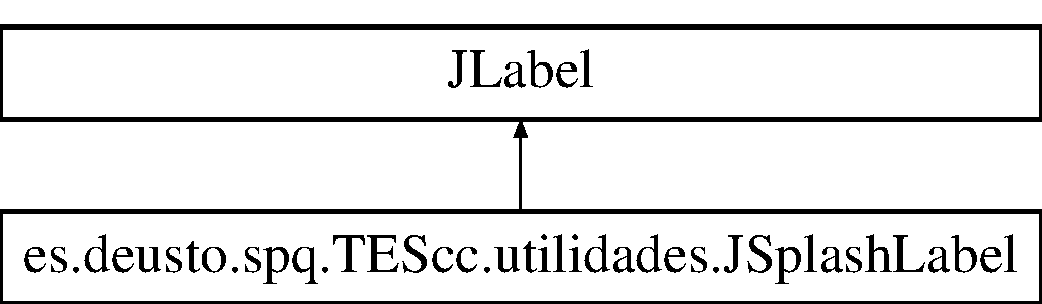
\includegraphics[height=2.000000cm]{classes_1_1deusto_1_1spq_1_1_t_e_scc_1_1utilidades_1_1_j_splash_label}
\end{center}
\end{figure}
\subsection*{Métodos públicos}
\begin{DoxyCompactItemize}
\item 
\hyperlink{classes_1_1deusto_1_1spq_1_1_t_e_scc_1_1utilidades_1_1_j_splash_label_aac19716284f0994f725dfd9999d7a5cc}{J\+Splash\+Label} (String path, String s, Font f, Color c)
\item 
\hyperlink{classes_1_1deusto_1_1spq_1_1_t_e_scc_1_1utilidades_1_1_j_splash_label_a2ddd9035e9bc35afa0252bf1fb71ef1c}{J\+Splash\+Label} (U\+R\+L url, String s)
\item 
void \hyperlink{classes_1_1deusto_1_1spq_1_1_t_e_scc_1_1utilidades_1_1_j_splash_label_ad4c20dc8708d554e0e1c181b026f94db}{paint} (Graphics g)
\end{DoxyCompactItemize}


\subsection{Descripción detallada}


Definición en la línea 15 del archivo J\+Splash\+Label.\+java.



\subsection{Documentación del constructor y destructor}
\hypertarget{classes_1_1deusto_1_1spq_1_1_t_e_scc_1_1utilidades_1_1_j_splash_label_aac19716284f0994f725dfd9999d7a5cc}{\index{es\+::deusto\+::spq\+::\+T\+E\+Scc\+::utilidades\+::\+J\+Splash\+Label@{es\+::deusto\+::spq\+::\+T\+E\+Scc\+::utilidades\+::\+J\+Splash\+Label}!J\+Splash\+Label@{J\+Splash\+Label}}
\index{J\+Splash\+Label@{J\+Splash\+Label}!es\+::deusto\+::spq\+::\+T\+E\+Scc\+::utilidades\+::\+J\+Splash\+Label@{es\+::deusto\+::spq\+::\+T\+E\+Scc\+::utilidades\+::\+J\+Splash\+Label}}
\subsubsection[{J\+Splash\+Label}]{\setlength{\rightskip}{0pt plus 5cm}es.\+deusto.\+spq.\+T\+E\+Scc.\+utilidades.\+J\+Splash\+Label.\+J\+Splash\+Label (
\begin{DoxyParamCaption}
\item[{String}]{path, }
\item[{String}]{s, }
\item[{Font}]{f, }
\item[{Color}]{c}
\end{DoxyParamCaption}
)}}\label{classes_1_1deusto_1_1spq_1_1_t_e_scc_1_1utilidades_1_1_j_splash_label_aac19716284f0994f725dfd9999d7a5cc}


Definición en la línea 26 del archivo J\+Splash\+Label.\+java.

\hypertarget{classes_1_1deusto_1_1spq_1_1_t_e_scc_1_1utilidades_1_1_j_splash_label_a2ddd9035e9bc35afa0252bf1fb71ef1c}{\index{es\+::deusto\+::spq\+::\+T\+E\+Scc\+::utilidades\+::\+J\+Splash\+Label@{es\+::deusto\+::spq\+::\+T\+E\+Scc\+::utilidades\+::\+J\+Splash\+Label}!J\+Splash\+Label@{J\+Splash\+Label}}
\index{J\+Splash\+Label@{J\+Splash\+Label}!es\+::deusto\+::spq\+::\+T\+E\+Scc\+::utilidades\+::\+J\+Splash\+Label@{es\+::deusto\+::spq\+::\+T\+E\+Scc\+::utilidades\+::\+J\+Splash\+Label}}
\subsubsection[{J\+Splash\+Label}]{\setlength{\rightskip}{0pt plus 5cm}es.\+deusto.\+spq.\+T\+E\+Scc.\+utilidades.\+J\+Splash\+Label.\+J\+Splash\+Label (
\begin{DoxyParamCaption}
\item[{U\+R\+L}]{url, }
\item[{String}]{s}
\end{DoxyParamCaption}
)}}\label{classes_1_1deusto_1_1spq_1_1_t_e_scc_1_1utilidades_1_1_j_splash_label_a2ddd9035e9bc35afa0252bf1fb71ef1c}


Definición en la línea 43 del archivo J\+Splash\+Label.\+java.



\subsection{Documentación de las funciones miembro}
\hypertarget{classes_1_1deusto_1_1spq_1_1_t_e_scc_1_1utilidades_1_1_j_splash_label_ad4c20dc8708d554e0e1c181b026f94db}{\index{es\+::deusto\+::spq\+::\+T\+E\+Scc\+::utilidades\+::\+J\+Splash\+Label@{es\+::deusto\+::spq\+::\+T\+E\+Scc\+::utilidades\+::\+J\+Splash\+Label}!paint@{paint}}
\index{paint@{paint}!es\+::deusto\+::spq\+::\+T\+E\+Scc\+::utilidades\+::\+J\+Splash\+Label@{es\+::deusto\+::spq\+::\+T\+E\+Scc\+::utilidades\+::\+J\+Splash\+Label}}
\subsubsection[{paint}]{\setlength{\rightskip}{0pt plus 5cm}void es.\+deusto.\+spq.\+T\+E\+Scc.\+utilidades.\+J\+Splash\+Label.\+paint (
\begin{DoxyParamCaption}
\item[{Graphics}]{g}
\end{DoxyParamCaption}
)}}\label{classes_1_1deusto_1_1spq_1_1_t_e_scc_1_1utilidades_1_1_j_splash_label_ad4c20dc8708d554e0e1c181b026f94db}


Definición en la línea 57 del archivo J\+Splash\+Label.\+java.



La documentación para esta clase fue generada a partir del siguiente fichero\+:\begin{DoxyCompactItemize}
\item 
src/main/java/es/deusto/spq/\+T\+E\+Scc/utilidades/\hyperlink{_j_splash_label_8java}{J\+Splash\+Label.\+java}\end{DoxyCompactItemize}

\hypertarget{classes_1_1deusto_1_1spq_1_1_t_e_scc_1_1ventanas_1_1_menu_personaje}{\section{Referencia de la Clase es.\+deusto.\+spq.\+T\+E\+Scc.\+ventanas.\+Menu\+Personaje}
\label{classes_1_1deusto_1_1spq_1_1_t_e_scc_1_1ventanas_1_1_menu_personaje}\index{es.\+deusto.\+spq.\+T\+E\+Scc.\+ventanas.\+Menu\+Personaje@{es.\+deusto.\+spq.\+T\+E\+Scc.\+ventanas.\+Menu\+Personaje}}
}
Diagrama de herencias de es.\+deusto.\+spq.\+T\+E\+Scc.\+ventanas.\+Menu\+Personaje\begin{figure}[H]
\begin{center}
\leavevmode
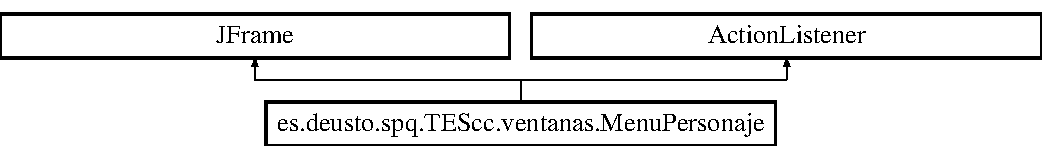
\includegraphics[height=1.958042cm]{classes_1_1deusto_1_1spq_1_1_t_e_scc_1_1ventanas_1_1_menu_personaje}
\end{center}
\end{figure}
\subsection*{Métodos públicos}
\begin{DoxyCompactItemize}
\item 
\hyperlink{classes_1_1deusto_1_1spq_1_1_t_e_scc_1_1ventanas_1_1_menu_personaje_a5ddd5cbbdb2d87f8541c37d2ae7feea6}{Menu\+Personaje} (String nombre\+Clase, String nom\+Usuario, String nom\+Personaje, \hyperlink{classes_1_1deusto_1_1spq_1_1_t_e_scc_1_1cliente_1_1_r_m_i_service_locator}{R\+M\+I\+Service\+Locator} rmi)
\item 
boolean \hyperlink{classes_1_1deusto_1_1spq_1_1_t_e_scc_1_1ventanas_1_1_menu_personaje_ad7ca7fcf44489ceacd767ad825eeb6b0}{existe\+Personaje} ()
\item 
void \hyperlink{classes_1_1deusto_1_1spq_1_1_t_e_scc_1_1ventanas_1_1_menu_personaje_ac085f2c43370fc01971bfa3e6097f768}{reiniciar\+Combo\+Boxes} ()
\item 
void \hyperlink{classes_1_1deusto_1_1spq_1_1_t_e_scc_1_1ventanas_1_1_menu_personaje_a87d4e80e81e4cb8a6ae23daa3b6e5938}{inizializar\+Hash\+Sets} ()
\item 
void \hyperlink{classes_1_1deusto_1_1spq_1_1_t_e_scc_1_1ventanas_1_1_menu_personaje_a9da923805fb3ea247a8332e9f56e7004}{inicializar\+Obejtos\+Per} ()  throws Remote\+Exception 
\item 
void \hyperlink{classes_1_1deusto_1_1spq_1_1_t_e_scc_1_1ventanas_1_1_menu_personaje_ad0936c89fc37412c29e22e9f415c4b4f}{inizializar\+Strings} ()
\item 
void \hyperlink{classes_1_1deusto_1_1spq_1_1_t_e_scc_1_1ventanas_1_1_menu_personaje_aa82435a6993747f7df4881f6eadf6609}{reiniciar\+Progress\+Bar} ()
\item 
void \hyperlink{classes_1_1deusto_1_1spq_1_1_t_e_scc_1_1ventanas_1_1_menu_personaje_a1fb433b9736274ac61537d826751e663}{actualizar\+Progress\+Bar} (String combo\+Box\+A\+Actualizar)
\item 
void \hyperlink{classes_1_1deusto_1_1spq_1_1_t_e_scc_1_1ventanas_1_1_menu_personaje_a3552e7ce3a5c41d17f1f29f7173363ae}{calcular\+Progress\+Bar} ()
\item 
void \hyperlink{classes_1_1deusto_1_1spq_1_1_t_e_scc_1_1ventanas_1_1_menu_personaje_a370d4d8f9ea3dc9d5cd421a44cce0983}{calcular\+Tipo} ()
\item 
String\mbox{[}$\,$\mbox{]} \hyperlink{classes_1_1deusto_1_1spq_1_1_t_e_scc_1_1ventanas_1_1_menu_personaje_a073e9dc8c06fec524a8e889723cf618e}{crear\+Lista} ()
\item 
String\mbox{[}$\,$\mbox{]} \hyperlink{classes_1_1deusto_1_1spq_1_1_t_e_scc_1_1ventanas_1_1_menu_personaje_ade52fe7d584c31499b7f0034f3f8f6d8}{volcar\+List\+A\+Aarray} (Linked\+List$<$ String $>$ lista)
\item 
String \hyperlink{classes_1_1deusto_1_1spq_1_1_t_e_scc_1_1ventanas_1_1_menu_personaje_a0bfab060e86fb75072be357901d71d81}{obtener\+Fecha\+Actual} ()
\item 
void \hyperlink{classes_1_1deusto_1_1spq_1_1_t_e_scc_1_1ventanas_1_1_menu_personaje_a2d37effefd80c5719805e02cc628e5fb}{action\+Performed} (Action\+Event e)
\end{DoxyCompactItemize}
\subsection*{Métodos públicos estáticos}
\begin{DoxyCompactItemize}
\item 
static void \hyperlink{classes_1_1deusto_1_1spq_1_1_t_e_scc_1_1ventanas_1_1_menu_personaje_abe4ae8888a5d91f7cad030cdf74bc285}{main} (String\mbox{[}$\,$\mbox{]} args)
\end{DoxyCompactItemize}


\subsection{Descripción detallada}


Definición en la línea 41 del archivo Menu\+Personaje.\+java.



\subsection{Documentación del constructor y destructor}
\hypertarget{classes_1_1deusto_1_1spq_1_1_t_e_scc_1_1ventanas_1_1_menu_personaje_a5ddd5cbbdb2d87f8541c37d2ae7feea6}{\index{es\+::deusto\+::spq\+::\+T\+E\+Scc\+::ventanas\+::\+Menu\+Personaje@{es\+::deusto\+::spq\+::\+T\+E\+Scc\+::ventanas\+::\+Menu\+Personaje}!Menu\+Personaje@{Menu\+Personaje}}
\index{Menu\+Personaje@{Menu\+Personaje}!es\+::deusto\+::spq\+::\+T\+E\+Scc\+::ventanas\+::\+Menu\+Personaje@{es\+::deusto\+::spq\+::\+T\+E\+Scc\+::ventanas\+::\+Menu\+Personaje}}
\subsubsection[{Menu\+Personaje}]{\setlength{\rightskip}{0pt plus 5cm}es.\+deusto.\+spq.\+T\+E\+Scc.\+ventanas.\+Menu\+Personaje.\+Menu\+Personaje (
\begin{DoxyParamCaption}
\item[{String}]{nombre\+Clase, }
\item[{String}]{nom\+Usuario, }
\item[{String}]{nom\+Personaje, }
\item[{{\bf R\+M\+I\+Service\+Locator}}]{rmi}
\end{DoxyParamCaption}
)}}\label{classes_1_1deusto_1_1spq_1_1_t_e_scc_1_1ventanas_1_1_menu_personaje_a5ddd5cbbdb2d87f8541c37d2ae7feea6}


Definición en la línea 100 del archivo Menu\+Personaje.\+java.



\subsection{Documentación de las funciones miembro}
\hypertarget{classes_1_1deusto_1_1spq_1_1_t_e_scc_1_1ventanas_1_1_menu_personaje_a2d37effefd80c5719805e02cc628e5fb}{\index{es\+::deusto\+::spq\+::\+T\+E\+Scc\+::ventanas\+::\+Menu\+Personaje@{es\+::deusto\+::spq\+::\+T\+E\+Scc\+::ventanas\+::\+Menu\+Personaje}!action\+Performed@{action\+Performed}}
\index{action\+Performed@{action\+Performed}!es\+::deusto\+::spq\+::\+T\+E\+Scc\+::ventanas\+::\+Menu\+Personaje@{es\+::deusto\+::spq\+::\+T\+E\+Scc\+::ventanas\+::\+Menu\+Personaje}}
\subsubsection[{action\+Performed}]{\setlength{\rightskip}{0pt plus 5cm}void es.\+deusto.\+spq.\+T\+E\+Scc.\+ventanas.\+Menu\+Personaje.\+action\+Performed (
\begin{DoxyParamCaption}
\item[{Action\+Event}]{e}
\end{DoxyParamCaption}
)}}\label{classes_1_1deusto_1_1spq_1_1_t_e_scc_1_1ventanas_1_1_menu_personaje_a2d37effefd80c5719805e02cc628e5fb}


Definición en la línea 643 del archivo Menu\+Personaje.\+java.

\hypertarget{classes_1_1deusto_1_1spq_1_1_t_e_scc_1_1ventanas_1_1_menu_personaje_a1fb433b9736274ac61537d826751e663}{\index{es\+::deusto\+::spq\+::\+T\+E\+Scc\+::ventanas\+::\+Menu\+Personaje@{es\+::deusto\+::spq\+::\+T\+E\+Scc\+::ventanas\+::\+Menu\+Personaje}!actualizar\+Progress\+Bar@{actualizar\+Progress\+Bar}}
\index{actualizar\+Progress\+Bar@{actualizar\+Progress\+Bar}!es\+::deusto\+::spq\+::\+T\+E\+Scc\+::ventanas\+::\+Menu\+Personaje@{es\+::deusto\+::spq\+::\+T\+E\+Scc\+::ventanas\+::\+Menu\+Personaje}}
\subsubsection[{actualizar\+Progress\+Bar}]{\setlength{\rightskip}{0pt plus 5cm}void es.\+deusto.\+spq.\+T\+E\+Scc.\+ventanas.\+Menu\+Personaje.\+actualizar\+Progress\+Bar (
\begin{DoxyParamCaption}
\item[{String}]{combo\+Box\+A\+Actualizar}
\end{DoxyParamCaption}
)}}\label{classes_1_1deusto_1_1spq_1_1_t_e_scc_1_1ventanas_1_1_menu_personaje_a1fb433b9736274ac61537d826751e663}


Definición en la línea 483 del archivo Menu\+Personaje.\+java.

\hypertarget{classes_1_1deusto_1_1spq_1_1_t_e_scc_1_1ventanas_1_1_menu_personaje_a3552e7ce3a5c41d17f1f29f7173363ae}{\index{es\+::deusto\+::spq\+::\+T\+E\+Scc\+::ventanas\+::\+Menu\+Personaje@{es\+::deusto\+::spq\+::\+T\+E\+Scc\+::ventanas\+::\+Menu\+Personaje}!calcular\+Progress\+Bar@{calcular\+Progress\+Bar}}
\index{calcular\+Progress\+Bar@{calcular\+Progress\+Bar}!es\+::deusto\+::spq\+::\+T\+E\+Scc\+::ventanas\+::\+Menu\+Personaje@{es\+::deusto\+::spq\+::\+T\+E\+Scc\+::ventanas\+::\+Menu\+Personaje}}
\subsubsection[{calcular\+Progress\+Bar}]{\setlength{\rightskip}{0pt plus 5cm}void es.\+deusto.\+spq.\+T\+E\+Scc.\+ventanas.\+Menu\+Personaje.\+calcular\+Progress\+Bar (
\begin{DoxyParamCaption}
{}
\end{DoxyParamCaption}
)}}\label{classes_1_1deusto_1_1spq_1_1_t_e_scc_1_1ventanas_1_1_menu_personaje_a3552e7ce3a5c41d17f1f29f7173363ae}


Definición en la línea 546 del archivo Menu\+Personaje.\+java.

\hypertarget{classes_1_1deusto_1_1spq_1_1_t_e_scc_1_1ventanas_1_1_menu_personaje_a370d4d8f9ea3dc9d5cd421a44cce0983}{\index{es\+::deusto\+::spq\+::\+T\+E\+Scc\+::ventanas\+::\+Menu\+Personaje@{es\+::deusto\+::spq\+::\+T\+E\+Scc\+::ventanas\+::\+Menu\+Personaje}!calcular\+Tipo@{calcular\+Tipo}}
\index{calcular\+Tipo@{calcular\+Tipo}!es\+::deusto\+::spq\+::\+T\+E\+Scc\+::ventanas\+::\+Menu\+Personaje@{es\+::deusto\+::spq\+::\+T\+E\+Scc\+::ventanas\+::\+Menu\+Personaje}}
\subsubsection[{calcular\+Tipo}]{\setlength{\rightskip}{0pt plus 5cm}void es.\+deusto.\+spq.\+T\+E\+Scc.\+ventanas.\+Menu\+Personaje.\+calcular\+Tipo (
\begin{DoxyParamCaption}
{}
\end{DoxyParamCaption}
)}}\label{classes_1_1deusto_1_1spq_1_1_t_e_scc_1_1ventanas_1_1_menu_personaje_a370d4d8f9ea3dc9d5cd421a44cce0983}


Definición en la línea 603 del archivo Menu\+Personaje.\+java.

\hypertarget{classes_1_1deusto_1_1spq_1_1_t_e_scc_1_1ventanas_1_1_menu_personaje_a073e9dc8c06fec524a8e889723cf618e}{\index{es\+::deusto\+::spq\+::\+T\+E\+Scc\+::ventanas\+::\+Menu\+Personaje@{es\+::deusto\+::spq\+::\+T\+E\+Scc\+::ventanas\+::\+Menu\+Personaje}!crear\+Lista@{crear\+Lista}}
\index{crear\+Lista@{crear\+Lista}!es\+::deusto\+::spq\+::\+T\+E\+Scc\+::ventanas\+::\+Menu\+Personaje@{es\+::deusto\+::spq\+::\+T\+E\+Scc\+::ventanas\+::\+Menu\+Personaje}}
\subsubsection[{crear\+Lista}]{\setlength{\rightskip}{0pt plus 5cm}String \mbox{[}$\,$\mbox{]} es.\+deusto.\+spq.\+T\+E\+Scc.\+ventanas.\+Menu\+Personaje.\+crear\+Lista (
\begin{DoxyParamCaption}
{}
\end{DoxyParamCaption}
)}}\label{classes_1_1deusto_1_1spq_1_1_t_e_scc_1_1ventanas_1_1_menu_personaje_a073e9dc8c06fec524a8e889723cf618e}


Definición en la línea 613 del archivo Menu\+Personaje.\+java.

\hypertarget{classes_1_1deusto_1_1spq_1_1_t_e_scc_1_1ventanas_1_1_menu_personaje_ad7ca7fcf44489ceacd767ad825eeb6b0}{\index{es\+::deusto\+::spq\+::\+T\+E\+Scc\+::ventanas\+::\+Menu\+Personaje@{es\+::deusto\+::spq\+::\+T\+E\+Scc\+::ventanas\+::\+Menu\+Personaje}!existe\+Personaje@{existe\+Personaje}}
\index{existe\+Personaje@{existe\+Personaje}!es\+::deusto\+::spq\+::\+T\+E\+Scc\+::ventanas\+::\+Menu\+Personaje@{es\+::deusto\+::spq\+::\+T\+E\+Scc\+::ventanas\+::\+Menu\+Personaje}}
\subsubsection[{existe\+Personaje}]{\setlength{\rightskip}{0pt plus 5cm}boolean es.\+deusto.\+spq.\+T\+E\+Scc.\+ventanas.\+Menu\+Personaje.\+existe\+Personaje (
\begin{DoxyParamCaption}
{}
\end{DoxyParamCaption}
)}}\label{classes_1_1deusto_1_1spq_1_1_t_e_scc_1_1ventanas_1_1_menu_personaje_ad7ca7fcf44489ceacd767ad825eeb6b0}


Definición en la línea 384 del archivo Menu\+Personaje.\+java.

\hypertarget{classes_1_1deusto_1_1spq_1_1_t_e_scc_1_1ventanas_1_1_menu_personaje_a9da923805fb3ea247a8332e9f56e7004}{\index{es\+::deusto\+::spq\+::\+T\+E\+Scc\+::ventanas\+::\+Menu\+Personaje@{es\+::deusto\+::spq\+::\+T\+E\+Scc\+::ventanas\+::\+Menu\+Personaje}!inicializar\+Obejtos\+Per@{inicializar\+Obejtos\+Per}}
\index{inicializar\+Obejtos\+Per@{inicializar\+Obejtos\+Per}!es\+::deusto\+::spq\+::\+T\+E\+Scc\+::ventanas\+::\+Menu\+Personaje@{es\+::deusto\+::spq\+::\+T\+E\+Scc\+::ventanas\+::\+Menu\+Personaje}}
\subsubsection[{inicializar\+Obejtos\+Per}]{\setlength{\rightskip}{0pt plus 5cm}void es.\+deusto.\+spq.\+T\+E\+Scc.\+ventanas.\+Menu\+Personaje.\+inicializar\+Obejtos\+Per (
\begin{DoxyParamCaption}
{}
\end{DoxyParamCaption}
) throws Remote\+Exception}}\label{classes_1_1deusto_1_1spq_1_1_t_e_scc_1_1ventanas_1_1_menu_personaje_a9da923805fb3ea247a8332e9f56e7004}


Definición en la línea 423 del archivo Menu\+Personaje.\+java.

\hypertarget{classes_1_1deusto_1_1spq_1_1_t_e_scc_1_1ventanas_1_1_menu_personaje_a87d4e80e81e4cb8a6ae23daa3b6e5938}{\index{es\+::deusto\+::spq\+::\+T\+E\+Scc\+::ventanas\+::\+Menu\+Personaje@{es\+::deusto\+::spq\+::\+T\+E\+Scc\+::ventanas\+::\+Menu\+Personaje}!inizializar\+Hash\+Sets@{inizializar\+Hash\+Sets}}
\index{inizializar\+Hash\+Sets@{inizializar\+Hash\+Sets}!es\+::deusto\+::spq\+::\+T\+E\+Scc\+::ventanas\+::\+Menu\+Personaje@{es\+::deusto\+::spq\+::\+T\+E\+Scc\+::ventanas\+::\+Menu\+Personaje}}
\subsubsection[{inizializar\+Hash\+Sets}]{\setlength{\rightskip}{0pt plus 5cm}void es.\+deusto.\+spq.\+T\+E\+Scc.\+ventanas.\+Menu\+Personaje.\+inizializar\+Hash\+Sets (
\begin{DoxyParamCaption}
{}
\end{DoxyParamCaption}
)}}\label{classes_1_1deusto_1_1spq_1_1_t_e_scc_1_1ventanas_1_1_menu_personaje_a87d4e80e81e4cb8a6ae23daa3b6e5938}


Definición en la línea 407 del archivo Menu\+Personaje.\+java.

\hypertarget{classes_1_1deusto_1_1spq_1_1_t_e_scc_1_1ventanas_1_1_menu_personaje_ad0936c89fc37412c29e22e9f415c4b4f}{\index{es\+::deusto\+::spq\+::\+T\+E\+Scc\+::ventanas\+::\+Menu\+Personaje@{es\+::deusto\+::spq\+::\+T\+E\+Scc\+::ventanas\+::\+Menu\+Personaje}!inizializar\+Strings@{inizializar\+Strings}}
\index{inizializar\+Strings@{inizializar\+Strings}!es\+::deusto\+::spq\+::\+T\+E\+Scc\+::ventanas\+::\+Menu\+Personaje@{es\+::deusto\+::spq\+::\+T\+E\+Scc\+::ventanas\+::\+Menu\+Personaje}}
\subsubsection[{inizializar\+Strings}]{\setlength{\rightskip}{0pt plus 5cm}void es.\+deusto.\+spq.\+T\+E\+Scc.\+ventanas.\+Menu\+Personaje.\+inizializar\+Strings (
\begin{DoxyParamCaption}
{}
\end{DoxyParamCaption}
)}}\label{classes_1_1deusto_1_1spq_1_1_t_e_scc_1_1ventanas_1_1_menu_personaje_ad0936c89fc37412c29e22e9f415c4b4f}


Definición en la línea 444 del archivo Menu\+Personaje.\+java.

\hypertarget{classes_1_1deusto_1_1spq_1_1_t_e_scc_1_1ventanas_1_1_menu_personaje_abe4ae8888a5d91f7cad030cdf74bc285}{\index{es\+::deusto\+::spq\+::\+T\+E\+Scc\+::ventanas\+::\+Menu\+Personaje@{es\+::deusto\+::spq\+::\+T\+E\+Scc\+::ventanas\+::\+Menu\+Personaje}!main@{main}}
\index{main@{main}!es\+::deusto\+::spq\+::\+T\+E\+Scc\+::ventanas\+::\+Menu\+Personaje@{es\+::deusto\+::spq\+::\+T\+E\+Scc\+::ventanas\+::\+Menu\+Personaje}}
\subsubsection[{main}]{\setlength{\rightskip}{0pt plus 5cm}static void es.\+deusto.\+spq.\+T\+E\+Scc.\+ventanas.\+Menu\+Personaje.\+main (
\begin{DoxyParamCaption}
\item[{String\mbox{[}$\,$\mbox{]}}]{args}
\end{DoxyParamCaption}
)\hspace{0.3cm}{\ttfamily [static]}}}\label{classes_1_1deusto_1_1spq_1_1_t_e_scc_1_1ventanas_1_1_menu_personaje_abe4ae8888a5d91f7cad030cdf74bc285}


Definición en la línea 87 del archivo Menu\+Personaje.\+java.

\hypertarget{classes_1_1deusto_1_1spq_1_1_t_e_scc_1_1ventanas_1_1_menu_personaje_a0bfab060e86fb75072be357901d71d81}{\index{es\+::deusto\+::spq\+::\+T\+E\+Scc\+::ventanas\+::\+Menu\+Personaje@{es\+::deusto\+::spq\+::\+T\+E\+Scc\+::ventanas\+::\+Menu\+Personaje}!obtener\+Fecha\+Actual@{obtener\+Fecha\+Actual}}
\index{obtener\+Fecha\+Actual@{obtener\+Fecha\+Actual}!es\+::deusto\+::spq\+::\+T\+E\+Scc\+::ventanas\+::\+Menu\+Personaje@{es\+::deusto\+::spq\+::\+T\+E\+Scc\+::ventanas\+::\+Menu\+Personaje}}
\subsubsection[{obtener\+Fecha\+Actual}]{\setlength{\rightskip}{0pt plus 5cm}String es.\+deusto.\+spq.\+T\+E\+Scc.\+ventanas.\+Menu\+Personaje.\+obtener\+Fecha\+Actual (
\begin{DoxyParamCaption}
{}
\end{DoxyParamCaption}
)}}\label{classes_1_1deusto_1_1spq_1_1_t_e_scc_1_1ventanas_1_1_menu_personaje_a0bfab060e86fb75072be357901d71d81}


Definición en la línea 630 del archivo Menu\+Personaje.\+java.

\hypertarget{classes_1_1deusto_1_1spq_1_1_t_e_scc_1_1ventanas_1_1_menu_personaje_ac085f2c43370fc01971bfa3e6097f768}{\index{es\+::deusto\+::spq\+::\+T\+E\+Scc\+::ventanas\+::\+Menu\+Personaje@{es\+::deusto\+::spq\+::\+T\+E\+Scc\+::ventanas\+::\+Menu\+Personaje}!reiniciar\+Combo\+Boxes@{reiniciar\+Combo\+Boxes}}
\index{reiniciar\+Combo\+Boxes@{reiniciar\+Combo\+Boxes}!es\+::deusto\+::spq\+::\+T\+E\+Scc\+::ventanas\+::\+Menu\+Personaje@{es\+::deusto\+::spq\+::\+T\+E\+Scc\+::ventanas\+::\+Menu\+Personaje}}
\subsubsection[{reiniciar\+Combo\+Boxes}]{\setlength{\rightskip}{0pt plus 5cm}void es.\+deusto.\+spq.\+T\+E\+Scc.\+ventanas.\+Menu\+Personaje.\+reiniciar\+Combo\+Boxes (
\begin{DoxyParamCaption}
{}
\end{DoxyParamCaption}
)}}\label{classes_1_1deusto_1_1spq_1_1_t_e_scc_1_1ventanas_1_1_menu_personaje_ac085f2c43370fc01971bfa3e6097f768}


Definición en la línea 399 del archivo Menu\+Personaje.\+java.

\hypertarget{classes_1_1deusto_1_1spq_1_1_t_e_scc_1_1ventanas_1_1_menu_personaje_aa82435a6993747f7df4881f6eadf6609}{\index{es\+::deusto\+::spq\+::\+T\+E\+Scc\+::ventanas\+::\+Menu\+Personaje@{es\+::deusto\+::spq\+::\+T\+E\+Scc\+::ventanas\+::\+Menu\+Personaje}!reiniciar\+Progress\+Bar@{reiniciar\+Progress\+Bar}}
\index{reiniciar\+Progress\+Bar@{reiniciar\+Progress\+Bar}!es\+::deusto\+::spq\+::\+T\+E\+Scc\+::ventanas\+::\+Menu\+Personaje@{es\+::deusto\+::spq\+::\+T\+E\+Scc\+::ventanas\+::\+Menu\+Personaje}}
\subsubsection[{reiniciar\+Progress\+Bar}]{\setlength{\rightskip}{0pt plus 5cm}void es.\+deusto.\+spq.\+T\+E\+Scc.\+ventanas.\+Menu\+Personaje.\+reiniciar\+Progress\+Bar (
\begin{DoxyParamCaption}
{}
\end{DoxyParamCaption}
)}}\label{classes_1_1deusto_1_1spq_1_1_t_e_scc_1_1ventanas_1_1_menu_personaje_aa82435a6993747f7df4881f6eadf6609}


Definición en la línea 474 del archivo Menu\+Personaje.\+java.

\hypertarget{classes_1_1deusto_1_1spq_1_1_t_e_scc_1_1ventanas_1_1_menu_personaje_ade52fe7d584c31499b7f0034f3f8f6d8}{\index{es\+::deusto\+::spq\+::\+T\+E\+Scc\+::ventanas\+::\+Menu\+Personaje@{es\+::deusto\+::spq\+::\+T\+E\+Scc\+::ventanas\+::\+Menu\+Personaje}!volcar\+List\+A\+Aarray@{volcar\+List\+A\+Aarray}}
\index{volcar\+List\+A\+Aarray@{volcar\+List\+A\+Aarray}!es\+::deusto\+::spq\+::\+T\+E\+Scc\+::ventanas\+::\+Menu\+Personaje@{es\+::deusto\+::spq\+::\+T\+E\+Scc\+::ventanas\+::\+Menu\+Personaje}}
\subsubsection[{volcar\+List\+A\+Aarray}]{\setlength{\rightskip}{0pt plus 5cm}String \mbox{[}$\,$\mbox{]} es.\+deusto.\+spq.\+T\+E\+Scc.\+ventanas.\+Menu\+Personaje.\+volcar\+List\+A\+Aarray (
\begin{DoxyParamCaption}
\item[{Linked\+List$<$ String $>$}]{lista}
\end{DoxyParamCaption}
)}}\label{classes_1_1deusto_1_1spq_1_1_t_e_scc_1_1ventanas_1_1_menu_personaje_ade52fe7d584c31499b7f0034f3f8f6d8}


Definición en la línea 622 del archivo Menu\+Personaje.\+java.



La documentación para esta clase fue generada a partir del siguiente fichero\+:\begin{DoxyCompactItemize}
\item 
src/main/java/es/deusto/spq/\+T\+E\+Scc/ventanas/\hyperlink{_menu_personaje_8java}{Menu\+Personaje.\+java}\end{DoxyCompactItemize}

\hypertarget{classes_1_1deusto_1_1spq_1_1_t_e_scc_1_1servidor_1_1jdo_1_1_objeto}{\section{Referencia de la Clase es.\+deusto.\+spq.\+T\+E\+Scc.\+servidor.\+jdo.\+Objeto}
\label{classes_1_1deusto_1_1spq_1_1_t_e_scc_1_1servidor_1_1jdo_1_1_objeto}\index{es.\+deusto.\+spq.\+T\+E\+Scc.\+servidor.\+jdo.\+Objeto@{es.\+deusto.\+spq.\+T\+E\+Scc.\+servidor.\+jdo.\+Objeto}}
}
\subsection*{Métodos públicos}
\begin{DoxyCompactItemize}
\item 
\hyperlink{classes_1_1deusto_1_1spq_1_1_t_e_scc_1_1servidor_1_1jdo_1_1_objeto_ae1a67a6e5f6e14632ec622d5e8c3ef1d}{Objeto} ()
\item 
\hyperlink{classes_1_1deusto_1_1spq_1_1_t_e_scc_1_1servidor_1_1jdo_1_1_objeto_aa05dd1436222a60576fa7d6a4956e63b}{Objeto} (String nombre, int vida, int velocidad, int armadura, int discrecion, int ataque, int defensa, int tipo)
\item 
String \hyperlink{classes_1_1deusto_1_1spq_1_1_t_e_scc_1_1servidor_1_1jdo_1_1_objeto_ad677d91180ca77d2ba2d3e84524c9023}{get\+Nombre} ()
\item 
void \hyperlink{classes_1_1deusto_1_1spq_1_1_t_e_scc_1_1servidor_1_1jdo_1_1_objeto_aa36e75ff0feb1e50292bba4bfdaffa99}{set\+Nombre} (String nombre)
\item 
int \hyperlink{classes_1_1deusto_1_1spq_1_1_t_e_scc_1_1servidor_1_1jdo_1_1_objeto_a40079a07ad9ee70cfef818601a52e5a1}{get\+Vida} ()
\item 
void \hyperlink{classes_1_1deusto_1_1spq_1_1_t_e_scc_1_1servidor_1_1jdo_1_1_objeto_a528ca922ef15618d4baef73e2de4a4de}{set\+Vida} (int vida)
\item 
int \hyperlink{classes_1_1deusto_1_1spq_1_1_t_e_scc_1_1servidor_1_1jdo_1_1_objeto_ad6edabe746803dc65fc9c7705aa8ac7d}{get\+Velocidad} ()
\item 
void \hyperlink{classes_1_1deusto_1_1spq_1_1_t_e_scc_1_1servidor_1_1jdo_1_1_objeto_a3d88780721f80ee28b41526297cd5a3a}{set\+Velocidad} (int velocidad)
\item 
int \hyperlink{classes_1_1deusto_1_1spq_1_1_t_e_scc_1_1servidor_1_1jdo_1_1_objeto_ae4297a07383ea9da8319c8fe5da18266}{get\+Armadura} ()
\item 
void \hyperlink{classes_1_1deusto_1_1spq_1_1_t_e_scc_1_1servidor_1_1jdo_1_1_objeto_ad95d13fbd823ea147a1b405147ff70b8}{set\+Armadura} (int armadura)
\item 
int \hyperlink{classes_1_1deusto_1_1spq_1_1_t_e_scc_1_1servidor_1_1jdo_1_1_objeto_a6b8cc4c28ba9cac790830d16cea7f6ed}{get\+Discrecion} ()
\item 
void \hyperlink{classes_1_1deusto_1_1spq_1_1_t_e_scc_1_1servidor_1_1jdo_1_1_objeto_a356a151fe13b62442cccedc64d314c20}{set\+Discrecion} (int discrecion)
\item 
int \hyperlink{classes_1_1deusto_1_1spq_1_1_t_e_scc_1_1servidor_1_1jdo_1_1_objeto_a6341bc39a45e9ecdf395ffe103b82531}{get\+Ataque} ()
\item 
void \hyperlink{classes_1_1deusto_1_1spq_1_1_t_e_scc_1_1servidor_1_1jdo_1_1_objeto_ad6ce4904119eb800f3a1c0c24250a6f5}{set\+Ataque} (int ataque)
\item 
int \hyperlink{classes_1_1deusto_1_1spq_1_1_t_e_scc_1_1servidor_1_1jdo_1_1_objeto_a5ec769efb59a2a1dc55144eaba73b311}{get\+Defensa} ()
\item 
void \hyperlink{classes_1_1deusto_1_1spq_1_1_t_e_scc_1_1servidor_1_1jdo_1_1_objeto_ae1c7efccb2567e4e472a61b323491141}{set\+Defensa} (int defensa)
\item 
int \hyperlink{classes_1_1deusto_1_1spq_1_1_t_e_scc_1_1servidor_1_1jdo_1_1_objeto_ab8772c99abed2a763eb343cd6c238414}{get\+Tipo} ()
\item 
void \hyperlink{classes_1_1deusto_1_1spq_1_1_t_e_scc_1_1servidor_1_1jdo_1_1_objeto_acccbde3b5d80065e203cb6677830a247}{set\+Tipo} (int tipo)
\item 
void \hyperlink{classes_1_1deusto_1_1spq_1_1_t_e_scc_1_1servidor_1_1jdo_1_1_objeto_a9c7cfca0877b8dd023ca3833ccb5f7f6}{aniadir\+Personaje} (\hyperlink{classes_1_1deusto_1_1spq_1_1_t_e_scc_1_1servidor_1_1jdo_1_1_personaje}{Personaje} personaje)
\item 
void \hyperlink{classes_1_1deusto_1_1spq_1_1_t_e_scc_1_1servidor_1_1jdo_1_1_objeto_a44dc9a7acce28cfd24a646d47fd7876c}{eliminar\+Personaje} (\hyperlink{classes_1_1deusto_1_1spq_1_1_t_e_scc_1_1servidor_1_1jdo_1_1_personaje}{Personaje} personaje)
\item 
int \hyperlink{classes_1_1deusto_1_1spq_1_1_t_e_scc_1_1servidor_1_1jdo_1_1_objeto_a5fbc1d7943fd58c723ef15d0899c0dfa}{numero\+De\+Personajes} ()
\item 
Set$<$ \hyperlink{classes_1_1deusto_1_1spq_1_1_t_e_scc_1_1servidor_1_1jdo_1_1_personaje}{Personaje} $>$ \hyperlink{classes_1_1deusto_1_1spq_1_1_t_e_scc_1_1servidor_1_1jdo_1_1_objeto_ae18ab1ecc2cf933e9ed3a5adc29a80a7}{get\+Personajes} ()
\item 
void \hyperlink{classes_1_1deusto_1_1spq_1_1_t_e_scc_1_1servidor_1_1jdo_1_1_objeto_a5790799c8cf861591bc3257e0962c8b8}{set\+Personajes} (Set$<$ \hyperlink{classes_1_1deusto_1_1spq_1_1_t_e_scc_1_1servidor_1_1jdo_1_1_personaje}{Personaje} $>$ personajes)
\item 
boolean \hyperlink{classes_1_1deusto_1_1spq_1_1_t_e_scc_1_1servidor_1_1jdo_1_1_objeto_a2c4d0e2bb5773c8fc67b4705887b9416}{equals} (\hyperlink{classes_1_1deusto_1_1spq_1_1_t_e_scc_1_1servidor_1_1jdo_1_1_objeto}{Objeto} objeto)
\end{DoxyCompactItemize}
\subsection*{Atributos públicos estáticos}
\begin{DoxyCompactItemize}
\item 
static final int \hyperlink{classes_1_1deusto_1_1spq_1_1_t_e_scc_1_1servidor_1_1jdo_1_1_objeto_aad4056cca1c234c1388db2c39d542fa5}{Y\+E\+L\+M\+O} = 0
\item 
static final int \hyperlink{classes_1_1deusto_1_1spq_1_1_t_e_scc_1_1servidor_1_1jdo_1_1_objeto_ae089b3cd9b53d0444e1e765a5a7d97d8}{A\+R\+M\+A\+D\+U\+R\+A} = 1
\item 
static final int \hyperlink{classes_1_1deusto_1_1spq_1_1_t_e_scc_1_1servidor_1_1jdo_1_1_objeto_ae1705e9f36a42915ac8792c4c564c544}{B\+R\+A\+Z\+A\+L\+E\+T\+E} = 2
\item 
static final int \hyperlink{classes_1_1deusto_1_1spq_1_1_t_e_scc_1_1servidor_1_1jdo_1_1_objeto_aa7f15eb9649a66e8d74e7875053fe229}{B\+O\+T\+A\+S} = 3
\end{DoxyCompactItemize}


\subsection{Descripción detallada}


Definición en la línea 9 del archivo Objeto.\+java.



\subsection{Documentación del constructor y destructor}
\hypertarget{classes_1_1deusto_1_1spq_1_1_t_e_scc_1_1servidor_1_1jdo_1_1_objeto_ae1a67a6e5f6e14632ec622d5e8c3ef1d}{\index{es\+::deusto\+::spq\+::\+T\+E\+Scc\+::servidor\+::jdo\+::\+Objeto@{es\+::deusto\+::spq\+::\+T\+E\+Scc\+::servidor\+::jdo\+::\+Objeto}!Objeto@{Objeto}}
\index{Objeto@{Objeto}!es\+::deusto\+::spq\+::\+T\+E\+Scc\+::servidor\+::jdo\+::\+Objeto@{es\+::deusto\+::spq\+::\+T\+E\+Scc\+::servidor\+::jdo\+::\+Objeto}}
\subsubsection[{Objeto}]{\setlength{\rightskip}{0pt plus 5cm}es.\+deusto.\+spq.\+T\+E\+Scc.\+servidor.\+jdo.\+Objeto.\+Objeto (
\begin{DoxyParamCaption}
{}
\end{DoxyParamCaption}
)}}\label{classes_1_1deusto_1_1spq_1_1_t_e_scc_1_1servidor_1_1jdo_1_1_objeto_ae1a67a6e5f6e14632ec622d5e8c3ef1d}


Definición en la línea 26 del archivo Objeto.\+java.

\hypertarget{classes_1_1deusto_1_1spq_1_1_t_e_scc_1_1servidor_1_1jdo_1_1_objeto_aa05dd1436222a60576fa7d6a4956e63b}{\index{es\+::deusto\+::spq\+::\+T\+E\+Scc\+::servidor\+::jdo\+::\+Objeto@{es\+::deusto\+::spq\+::\+T\+E\+Scc\+::servidor\+::jdo\+::\+Objeto}!Objeto@{Objeto}}
\index{Objeto@{Objeto}!es\+::deusto\+::spq\+::\+T\+E\+Scc\+::servidor\+::jdo\+::\+Objeto@{es\+::deusto\+::spq\+::\+T\+E\+Scc\+::servidor\+::jdo\+::\+Objeto}}
\subsubsection[{Objeto}]{\setlength{\rightskip}{0pt plus 5cm}es.\+deusto.\+spq.\+T\+E\+Scc.\+servidor.\+jdo.\+Objeto.\+Objeto (
\begin{DoxyParamCaption}
\item[{String}]{nombre, }
\item[{int}]{vida, }
\item[{int}]{velocidad, }
\item[{int}]{armadura, }
\item[{int}]{discrecion, }
\item[{int}]{ataque, }
\item[{int}]{defensa, }
\item[{int}]{tipo}
\end{DoxyParamCaption}
)}}\label{classes_1_1deusto_1_1spq_1_1_t_e_scc_1_1servidor_1_1jdo_1_1_objeto_aa05dd1436222a60576fa7d6a4956e63b}


Definición en la línea 29 del archivo Objeto.\+java.



\subsection{Documentación de las funciones miembro}
\hypertarget{classes_1_1deusto_1_1spq_1_1_t_e_scc_1_1servidor_1_1jdo_1_1_objeto_a9c7cfca0877b8dd023ca3833ccb5f7f6}{\index{es\+::deusto\+::spq\+::\+T\+E\+Scc\+::servidor\+::jdo\+::\+Objeto@{es\+::deusto\+::spq\+::\+T\+E\+Scc\+::servidor\+::jdo\+::\+Objeto}!aniadir\+Personaje@{aniadir\+Personaje}}
\index{aniadir\+Personaje@{aniadir\+Personaje}!es\+::deusto\+::spq\+::\+T\+E\+Scc\+::servidor\+::jdo\+::\+Objeto@{es\+::deusto\+::spq\+::\+T\+E\+Scc\+::servidor\+::jdo\+::\+Objeto}}
\subsubsection[{aniadir\+Personaje}]{\setlength{\rightskip}{0pt plus 5cm}void es.\+deusto.\+spq.\+T\+E\+Scc.\+servidor.\+jdo.\+Objeto.\+aniadir\+Personaje (
\begin{DoxyParamCaption}
\item[{{\bf Personaje}}]{personaje}
\end{DoxyParamCaption}
)}}\label{classes_1_1deusto_1_1spq_1_1_t_e_scc_1_1servidor_1_1jdo_1_1_objeto_a9c7cfca0877b8dd023ca3833ccb5f7f6}


Definición en la línea 105 del archivo Objeto.\+java.

\hypertarget{classes_1_1deusto_1_1spq_1_1_t_e_scc_1_1servidor_1_1jdo_1_1_objeto_a44dc9a7acce28cfd24a646d47fd7876c}{\index{es\+::deusto\+::spq\+::\+T\+E\+Scc\+::servidor\+::jdo\+::\+Objeto@{es\+::deusto\+::spq\+::\+T\+E\+Scc\+::servidor\+::jdo\+::\+Objeto}!eliminar\+Personaje@{eliminar\+Personaje}}
\index{eliminar\+Personaje@{eliminar\+Personaje}!es\+::deusto\+::spq\+::\+T\+E\+Scc\+::servidor\+::jdo\+::\+Objeto@{es\+::deusto\+::spq\+::\+T\+E\+Scc\+::servidor\+::jdo\+::\+Objeto}}
\subsubsection[{eliminar\+Personaje}]{\setlength{\rightskip}{0pt plus 5cm}void es.\+deusto.\+spq.\+T\+E\+Scc.\+servidor.\+jdo.\+Objeto.\+eliminar\+Personaje (
\begin{DoxyParamCaption}
\item[{{\bf Personaje}}]{personaje}
\end{DoxyParamCaption}
)}}\label{classes_1_1deusto_1_1spq_1_1_t_e_scc_1_1servidor_1_1jdo_1_1_objeto_a44dc9a7acce28cfd24a646d47fd7876c}


Definición en la línea 109 del archivo Objeto.\+java.

\hypertarget{classes_1_1deusto_1_1spq_1_1_t_e_scc_1_1servidor_1_1jdo_1_1_objeto_a2c4d0e2bb5773c8fc67b4705887b9416}{\index{es\+::deusto\+::spq\+::\+T\+E\+Scc\+::servidor\+::jdo\+::\+Objeto@{es\+::deusto\+::spq\+::\+T\+E\+Scc\+::servidor\+::jdo\+::\+Objeto}!equals@{equals}}
\index{equals@{equals}!es\+::deusto\+::spq\+::\+T\+E\+Scc\+::servidor\+::jdo\+::\+Objeto@{es\+::deusto\+::spq\+::\+T\+E\+Scc\+::servidor\+::jdo\+::\+Objeto}}
\subsubsection[{equals}]{\setlength{\rightskip}{0pt plus 5cm}boolean es.\+deusto.\+spq.\+T\+E\+Scc.\+servidor.\+jdo.\+Objeto.\+equals (
\begin{DoxyParamCaption}
\item[{{\bf Objeto}}]{objeto}
\end{DoxyParamCaption}
)}}\label{classes_1_1deusto_1_1spq_1_1_t_e_scc_1_1servidor_1_1jdo_1_1_objeto_a2c4d0e2bb5773c8fc67b4705887b9416}


Definición en la línea 125 del archivo Objeto.\+java.

\hypertarget{classes_1_1deusto_1_1spq_1_1_t_e_scc_1_1servidor_1_1jdo_1_1_objeto_ae4297a07383ea9da8319c8fe5da18266}{\index{es\+::deusto\+::spq\+::\+T\+E\+Scc\+::servidor\+::jdo\+::\+Objeto@{es\+::deusto\+::spq\+::\+T\+E\+Scc\+::servidor\+::jdo\+::\+Objeto}!get\+Armadura@{get\+Armadura}}
\index{get\+Armadura@{get\+Armadura}!es\+::deusto\+::spq\+::\+T\+E\+Scc\+::servidor\+::jdo\+::\+Objeto@{es\+::deusto\+::spq\+::\+T\+E\+Scc\+::servidor\+::jdo\+::\+Objeto}}
\subsubsection[{get\+Armadura}]{\setlength{\rightskip}{0pt plus 5cm}int es.\+deusto.\+spq.\+T\+E\+Scc.\+servidor.\+jdo.\+Objeto.\+get\+Armadura (
\begin{DoxyParamCaption}
{}
\end{DoxyParamCaption}
)}}\label{classes_1_1deusto_1_1spq_1_1_t_e_scc_1_1servidor_1_1jdo_1_1_objeto_ae4297a07383ea9da8319c8fe5da18266}


Definición en la línea 65 del archivo Objeto.\+java.

\hypertarget{classes_1_1deusto_1_1spq_1_1_t_e_scc_1_1servidor_1_1jdo_1_1_objeto_a6341bc39a45e9ecdf395ffe103b82531}{\index{es\+::deusto\+::spq\+::\+T\+E\+Scc\+::servidor\+::jdo\+::\+Objeto@{es\+::deusto\+::spq\+::\+T\+E\+Scc\+::servidor\+::jdo\+::\+Objeto}!get\+Ataque@{get\+Ataque}}
\index{get\+Ataque@{get\+Ataque}!es\+::deusto\+::spq\+::\+T\+E\+Scc\+::servidor\+::jdo\+::\+Objeto@{es\+::deusto\+::spq\+::\+T\+E\+Scc\+::servidor\+::jdo\+::\+Objeto}}
\subsubsection[{get\+Ataque}]{\setlength{\rightskip}{0pt plus 5cm}int es.\+deusto.\+spq.\+T\+E\+Scc.\+servidor.\+jdo.\+Objeto.\+get\+Ataque (
\begin{DoxyParamCaption}
{}
\end{DoxyParamCaption}
)}}\label{classes_1_1deusto_1_1spq_1_1_t_e_scc_1_1servidor_1_1jdo_1_1_objeto_a6341bc39a45e9ecdf395ffe103b82531}


Definición en la línea 81 del archivo Objeto.\+java.

\hypertarget{classes_1_1deusto_1_1spq_1_1_t_e_scc_1_1servidor_1_1jdo_1_1_objeto_a5ec769efb59a2a1dc55144eaba73b311}{\index{es\+::deusto\+::spq\+::\+T\+E\+Scc\+::servidor\+::jdo\+::\+Objeto@{es\+::deusto\+::spq\+::\+T\+E\+Scc\+::servidor\+::jdo\+::\+Objeto}!get\+Defensa@{get\+Defensa}}
\index{get\+Defensa@{get\+Defensa}!es\+::deusto\+::spq\+::\+T\+E\+Scc\+::servidor\+::jdo\+::\+Objeto@{es\+::deusto\+::spq\+::\+T\+E\+Scc\+::servidor\+::jdo\+::\+Objeto}}
\subsubsection[{get\+Defensa}]{\setlength{\rightskip}{0pt plus 5cm}int es.\+deusto.\+spq.\+T\+E\+Scc.\+servidor.\+jdo.\+Objeto.\+get\+Defensa (
\begin{DoxyParamCaption}
{}
\end{DoxyParamCaption}
)}}\label{classes_1_1deusto_1_1spq_1_1_t_e_scc_1_1servidor_1_1jdo_1_1_objeto_a5ec769efb59a2a1dc55144eaba73b311}


Definición en la línea 89 del archivo Objeto.\+java.

\hypertarget{classes_1_1deusto_1_1spq_1_1_t_e_scc_1_1servidor_1_1jdo_1_1_objeto_a6b8cc4c28ba9cac790830d16cea7f6ed}{\index{es\+::deusto\+::spq\+::\+T\+E\+Scc\+::servidor\+::jdo\+::\+Objeto@{es\+::deusto\+::spq\+::\+T\+E\+Scc\+::servidor\+::jdo\+::\+Objeto}!get\+Discrecion@{get\+Discrecion}}
\index{get\+Discrecion@{get\+Discrecion}!es\+::deusto\+::spq\+::\+T\+E\+Scc\+::servidor\+::jdo\+::\+Objeto@{es\+::deusto\+::spq\+::\+T\+E\+Scc\+::servidor\+::jdo\+::\+Objeto}}
\subsubsection[{get\+Discrecion}]{\setlength{\rightskip}{0pt plus 5cm}int es.\+deusto.\+spq.\+T\+E\+Scc.\+servidor.\+jdo.\+Objeto.\+get\+Discrecion (
\begin{DoxyParamCaption}
{}
\end{DoxyParamCaption}
)}}\label{classes_1_1deusto_1_1spq_1_1_t_e_scc_1_1servidor_1_1jdo_1_1_objeto_a6b8cc4c28ba9cac790830d16cea7f6ed}


Definición en la línea 73 del archivo Objeto.\+java.

\hypertarget{classes_1_1deusto_1_1spq_1_1_t_e_scc_1_1servidor_1_1jdo_1_1_objeto_ad677d91180ca77d2ba2d3e84524c9023}{\index{es\+::deusto\+::spq\+::\+T\+E\+Scc\+::servidor\+::jdo\+::\+Objeto@{es\+::deusto\+::spq\+::\+T\+E\+Scc\+::servidor\+::jdo\+::\+Objeto}!get\+Nombre@{get\+Nombre}}
\index{get\+Nombre@{get\+Nombre}!es\+::deusto\+::spq\+::\+T\+E\+Scc\+::servidor\+::jdo\+::\+Objeto@{es\+::deusto\+::spq\+::\+T\+E\+Scc\+::servidor\+::jdo\+::\+Objeto}}
\subsubsection[{get\+Nombre}]{\setlength{\rightskip}{0pt plus 5cm}String es.\+deusto.\+spq.\+T\+E\+Scc.\+servidor.\+jdo.\+Objeto.\+get\+Nombre (
\begin{DoxyParamCaption}
{}
\end{DoxyParamCaption}
)}}\label{classes_1_1deusto_1_1spq_1_1_t_e_scc_1_1servidor_1_1jdo_1_1_objeto_ad677d91180ca77d2ba2d3e84524c9023}


Definición en la línea 41 del archivo Objeto.\+java.

\hypertarget{classes_1_1deusto_1_1spq_1_1_t_e_scc_1_1servidor_1_1jdo_1_1_objeto_ae18ab1ecc2cf933e9ed3a5adc29a80a7}{\index{es\+::deusto\+::spq\+::\+T\+E\+Scc\+::servidor\+::jdo\+::\+Objeto@{es\+::deusto\+::spq\+::\+T\+E\+Scc\+::servidor\+::jdo\+::\+Objeto}!get\+Personajes@{get\+Personajes}}
\index{get\+Personajes@{get\+Personajes}!es\+::deusto\+::spq\+::\+T\+E\+Scc\+::servidor\+::jdo\+::\+Objeto@{es\+::deusto\+::spq\+::\+T\+E\+Scc\+::servidor\+::jdo\+::\+Objeto}}
\subsubsection[{get\+Personajes}]{\setlength{\rightskip}{0pt plus 5cm}Set$<${\bf Personaje}$>$ es.\+deusto.\+spq.\+T\+E\+Scc.\+servidor.\+jdo.\+Objeto.\+get\+Personajes (
\begin{DoxyParamCaption}
{}
\end{DoxyParamCaption}
)}}\label{classes_1_1deusto_1_1spq_1_1_t_e_scc_1_1servidor_1_1jdo_1_1_objeto_ae18ab1ecc2cf933e9ed3a5adc29a80a7}


Definición en la línea 117 del archivo Objeto.\+java.

\hypertarget{classes_1_1deusto_1_1spq_1_1_t_e_scc_1_1servidor_1_1jdo_1_1_objeto_ab8772c99abed2a763eb343cd6c238414}{\index{es\+::deusto\+::spq\+::\+T\+E\+Scc\+::servidor\+::jdo\+::\+Objeto@{es\+::deusto\+::spq\+::\+T\+E\+Scc\+::servidor\+::jdo\+::\+Objeto}!get\+Tipo@{get\+Tipo}}
\index{get\+Tipo@{get\+Tipo}!es\+::deusto\+::spq\+::\+T\+E\+Scc\+::servidor\+::jdo\+::\+Objeto@{es\+::deusto\+::spq\+::\+T\+E\+Scc\+::servidor\+::jdo\+::\+Objeto}}
\subsubsection[{get\+Tipo}]{\setlength{\rightskip}{0pt plus 5cm}int es.\+deusto.\+spq.\+T\+E\+Scc.\+servidor.\+jdo.\+Objeto.\+get\+Tipo (
\begin{DoxyParamCaption}
{}
\end{DoxyParamCaption}
)}}\label{classes_1_1deusto_1_1spq_1_1_t_e_scc_1_1servidor_1_1jdo_1_1_objeto_ab8772c99abed2a763eb343cd6c238414}


Definición en la línea 97 del archivo Objeto.\+java.

\hypertarget{classes_1_1deusto_1_1spq_1_1_t_e_scc_1_1servidor_1_1jdo_1_1_objeto_ad6edabe746803dc65fc9c7705aa8ac7d}{\index{es\+::deusto\+::spq\+::\+T\+E\+Scc\+::servidor\+::jdo\+::\+Objeto@{es\+::deusto\+::spq\+::\+T\+E\+Scc\+::servidor\+::jdo\+::\+Objeto}!get\+Velocidad@{get\+Velocidad}}
\index{get\+Velocidad@{get\+Velocidad}!es\+::deusto\+::spq\+::\+T\+E\+Scc\+::servidor\+::jdo\+::\+Objeto@{es\+::deusto\+::spq\+::\+T\+E\+Scc\+::servidor\+::jdo\+::\+Objeto}}
\subsubsection[{get\+Velocidad}]{\setlength{\rightskip}{0pt plus 5cm}int es.\+deusto.\+spq.\+T\+E\+Scc.\+servidor.\+jdo.\+Objeto.\+get\+Velocidad (
\begin{DoxyParamCaption}
{}
\end{DoxyParamCaption}
)}}\label{classes_1_1deusto_1_1spq_1_1_t_e_scc_1_1servidor_1_1jdo_1_1_objeto_ad6edabe746803dc65fc9c7705aa8ac7d}


Definición en la línea 57 del archivo Objeto.\+java.

\hypertarget{classes_1_1deusto_1_1spq_1_1_t_e_scc_1_1servidor_1_1jdo_1_1_objeto_a40079a07ad9ee70cfef818601a52e5a1}{\index{es\+::deusto\+::spq\+::\+T\+E\+Scc\+::servidor\+::jdo\+::\+Objeto@{es\+::deusto\+::spq\+::\+T\+E\+Scc\+::servidor\+::jdo\+::\+Objeto}!get\+Vida@{get\+Vida}}
\index{get\+Vida@{get\+Vida}!es\+::deusto\+::spq\+::\+T\+E\+Scc\+::servidor\+::jdo\+::\+Objeto@{es\+::deusto\+::spq\+::\+T\+E\+Scc\+::servidor\+::jdo\+::\+Objeto}}
\subsubsection[{get\+Vida}]{\setlength{\rightskip}{0pt plus 5cm}int es.\+deusto.\+spq.\+T\+E\+Scc.\+servidor.\+jdo.\+Objeto.\+get\+Vida (
\begin{DoxyParamCaption}
{}
\end{DoxyParamCaption}
)}}\label{classes_1_1deusto_1_1spq_1_1_t_e_scc_1_1servidor_1_1jdo_1_1_objeto_a40079a07ad9ee70cfef818601a52e5a1}


Definición en la línea 49 del archivo Objeto.\+java.

\hypertarget{classes_1_1deusto_1_1spq_1_1_t_e_scc_1_1servidor_1_1jdo_1_1_objeto_a5fbc1d7943fd58c723ef15d0899c0dfa}{\index{es\+::deusto\+::spq\+::\+T\+E\+Scc\+::servidor\+::jdo\+::\+Objeto@{es\+::deusto\+::spq\+::\+T\+E\+Scc\+::servidor\+::jdo\+::\+Objeto}!numero\+De\+Personajes@{numero\+De\+Personajes}}
\index{numero\+De\+Personajes@{numero\+De\+Personajes}!es\+::deusto\+::spq\+::\+T\+E\+Scc\+::servidor\+::jdo\+::\+Objeto@{es\+::deusto\+::spq\+::\+T\+E\+Scc\+::servidor\+::jdo\+::\+Objeto}}
\subsubsection[{numero\+De\+Personajes}]{\setlength{\rightskip}{0pt plus 5cm}int es.\+deusto.\+spq.\+T\+E\+Scc.\+servidor.\+jdo.\+Objeto.\+numero\+De\+Personajes (
\begin{DoxyParamCaption}
{}
\end{DoxyParamCaption}
)}}\label{classes_1_1deusto_1_1spq_1_1_t_e_scc_1_1servidor_1_1jdo_1_1_objeto_a5fbc1d7943fd58c723ef15d0899c0dfa}


Definición en la línea 113 del archivo Objeto.\+java.

\hypertarget{classes_1_1deusto_1_1spq_1_1_t_e_scc_1_1servidor_1_1jdo_1_1_objeto_ad95d13fbd823ea147a1b405147ff70b8}{\index{es\+::deusto\+::spq\+::\+T\+E\+Scc\+::servidor\+::jdo\+::\+Objeto@{es\+::deusto\+::spq\+::\+T\+E\+Scc\+::servidor\+::jdo\+::\+Objeto}!set\+Armadura@{set\+Armadura}}
\index{set\+Armadura@{set\+Armadura}!es\+::deusto\+::spq\+::\+T\+E\+Scc\+::servidor\+::jdo\+::\+Objeto@{es\+::deusto\+::spq\+::\+T\+E\+Scc\+::servidor\+::jdo\+::\+Objeto}}
\subsubsection[{set\+Armadura}]{\setlength{\rightskip}{0pt plus 5cm}void es.\+deusto.\+spq.\+T\+E\+Scc.\+servidor.\+jdo.\+Objeto.\+set\+Armadura (
\begin{DoxyParamCaption}
\item[{int}]{armadura}
\end{DoxyParamCaption}
)}}\label{classes_1_1deusto_1_1spq_1_1_t_e_scc_1_1servidor_1_1jdo_1_1_objeto_ad95d13fbd823ea147a1b405147ff70b8}


Definición en la línea 69 del archivo Objeto.\+java.

\hypertarget{classes_1_1deusto_1_1spq_1_1_t_e_scc_1_1servidor_1_1jdo_1_1_objeto_ad6ce4904119eb800f3a1c0c24250a6f5}{\index{es\+::deusto\+::spq\+::\+T\+E\+Scc\+::servidor\+::jdo\+::\+Objeto@{es\+::deusto\+::spq\+::\+T\+E\+Scc\+::servidor\+::jdo\+::\+Objeto}!set\+Ataque@{set\+Ataque}}
\index{set\+Ataque@{set\+Ataque}!es\+::deusto\+::spq\+::\+T\+E\+Scc\+::servidor\+::jdo\+::\+Objeto@{es\+::deusto\+::spq\+::\+T\+E\+Scc\+::servidor\+::jdo\+::\+Objeto}}
\subsubsection[{set\+Ataque}]{\setlength{\rightskip}{0pt plus 5cm}void es.\+deusto.\+spq.\+T\+E\+Scc.\+servidor.\+jdo.\+Objeto.\+set\+Ataque (
\begin{DoxyParamCaption}
\item[{int}]{ataque}
\end{DoxyParamCaption}
)}}\label{classes_1_1deusto_1_1spq_1_1_t_e_scc_1_1servidor_1_1jdo_1_1_objeto_ad6ce4904119eb800f3a1c0c24250a6f5}


Definición en la línea 85 del archivo Objeto.\+java.

\hypertarget{classes_1_1deusto_1_1spq_1_1_t_e_scc_1_1servidor_1_1jdo_1_1_objeto_ae1c7efccb2567e4e472a61b323491141}{\index{es\+::deusto\+::spq\+::\+T\+E\+Scc\+::servidor\+::jdo\+::\+Objeto@{es\+::deusto\+::spq\+::\+T\+E\+Scc\+::servidor\+::jdo\+::\+Objeto}!set\+Defensa@{set\+Defensa}}
\index{set\+Defensa@{set\+Defensa}!es\+::deusto\+::spq\+::\+T\+E\+Scc\+::servidor\+::jdo\+::\+Objeto@{es\+::deusto\+::spq\+::\+T\+E\+Scc\+::servidor\+::jdo\+::\+Objeto}}
\subsubsection[{set\+Defensa}]{\setlength{\rightskip}{0pt plus 5cm}void es.\+deusto.\+spq.\+T\+E\+Scc.\+servidor.\+jdo.\+Objeto.\+set\+Defensa (
\begin{DoxyParamCaption}
\item[{int}]{defensa}
\end{DoxyParamCaption}
)}}\label{classes_1_1deusto_1_1spq_1_1_t_e_scc_1_1servidor_1_1jdo_1_1_objeto_ae1c7efccb2567e4e472a61b323491141}


Definición en la línea 93 del archivo Objeto.\+java.

\hypertarget{classes_1_1deusto_1_1spq_1_1_t_e_scc_1_1servidor_1_1jdo_1_1_objeto_a356a151fe13b62442cccedc64d314c20}{\index{es\+::deusto\+::spq\+::\+T\+E\+Scc\+::servidor\+::jdo\+::\+Objeto@{es\+::deusto\+::spq\+::\+T\+E\+Scc\+::servidor\+::jdo\+::\+Objeto}!set\+Discrecion@{set\+Discrecion}}
\index{set\+Discrecion@{set\+Discrecion}!es\+::deusto\+::spq\+::\+T\+E\+Scc\+::servidor\+::jdo\+::\+Objeto@{es\+::deusto\+::spq\+::\+T\+E\+Scc\+::servidor\+::jdo\+::\+Objeto}}
\subsubsection[{set\+Discrecion}]{\setlength{\rightskip}{0pt plus 5cm}void es.\+deusto.\+spq.\+T\+E\+Scc.\+servidor.\+jdo.\+Objeto.\+set\+Discrecion (
\begin{DoxyParamCaption}
\item[{int}]{discrecion}
\end{DoxyParamCaption}
)}}\label{classes_1_1deusto_1_1spq_1_1_t_e_scc_1_1servidor_1_1jdo_1_1_objeto_a356a151fe13b62442cccedc64d314c20}


Definición en la línea 77 del archivo Objeto.\+java.

\hypertarget{classes_1_1deusto_1_1spq_1_1_t_e_scc_1_1servidor_1_1jdo_1_1_objeto_aa36e75ff0feb1e50292bba4bfdaffa99}{\index{es\+::deusto\+::spq\+::\+T\+E\+Scc\+::servidor\+::jdo\+::\+Objeto@{es\+::deusto\+::spq\+::\+T\+E\+Scc\+::servidor\+::jdo\+::\+Objeto}!set\+Nombre@{set\+Nombre}}
\index{set\+Nombre@{set\+Nombre}!es\+::deusto\+::spq\+::\+T\+E\+Scc\+::servidor\+::jdo\+::\+Objeto@{es\+::deusto\+::spq\+::\+T\+E\+Scc\+::servidor\+::jdo\+::\+Objeto}}
\subsubsection[{set\+Nombre}]{\setlength{\rightskip}{0pt plus 5cm}void es.\+deusto.\+spq.\+T\+E\+Scc.\+servidor.\+jdo.\+Objeto.\+set\+Nombre (
\begin{DoxyParamCaption}
\item[{String}]{nombre}
\end{DoxyParamCaption}
)}}\label{classes_1_1deusto_1_1spq_1_1_t_e_scc_1_1servidor_1_1jdo_1_1_objeto_aa36e75ff0feb1e50292bba4bfdaffa99}


Definición en la línea 45 del archivo Objeto.\+java.

\hypertarget{classes_1_1deusto_1_1spq_1_1_t_e_scc_1_1servidor_1_1jdo_1_1_objeto_a5790799c8cf861591bc3257e0962c8b8}{\index{es\+::deusto\+::spq\+::\+T\+E\+Scc\+::servidor\+::jdo\+::\+Objeto@{es\+::deusto\+::spq\+::\+T\+E\+Scc\+::servidor\+::jdo\+::\+Objeto}!set\+Personajes@{set\+Personajes}}
\index{set\+Personajes@{set\+Personajes}!es\+::deusto\+::spq\+::\+T\+E\+Scc\+::servidor\+::jdo\+::\+Objeto@{es\+::deusto\+::spq\+::\+T\+E\+Scc\+::servidor\+::jdo\+::\+Objeto}}
\subsubsection[{set\+Personajes}]{\setlength{\rightskip}{0pt plus 5cm}void es.\+deusto.\+spq.\+T\+E\+Scc.\+servidor.\+jdo.\+Objeto.\+set\+Personajes (
\begin{DoxyParamCaption}
\item[{Set$<$ {\bf Personaje} $>$}]{personajes}
\end{DoxyParamCaption}
)}}\label{classes_1_1deusto_1_1spq_1_1_t_e_scc_1_1servidor_1_1jdo_1_1_objeto_a5790799c8cf861591bc3257e0962c8b8}


Definición en la línea 121 del archivo Objeto.\+java.

\hypertarget{classes_1_1deusto_1_1spq_1_1_t_e_scc_1_1servidor_1_1jdo_1_1_objeto_acccbde3b5d80065e203cb6677830a247}{\index{es\+::deusto\+::spq\+::\+T\+E\+Scc\+::servidor\+::jdo\+::\+Objeto@{es\+::deusto\+::spq\+::\+T\+E\+Scc\+::servidor\+::jdo\+::\+Objeto}!set\+Tipo@{set\+Tipo}}
\index{set\+Tipo@{set\+Tipo}!es\+::deusto\+::spq\+::\+T\+E\+Scc\+::servidor\+::jdo\+::\+Objeto@{es\+::deusto\+::spq\+::\+T\+E\+Scc\+::servidor\+::jdo\+::\+Objeto}}
\subsubsection[{set\+Tipo}]{\setlength{\rightskip}{0pt plus 5cm}void es.\+deusto.\+spq.\+T\+E\+Scc.\+servidor.\+jdo.\+Objeto.\+set\+Tipo (
\begin{DoxyParamCaption}
\item[{int}]{tipo}
\end{DoxyParamCaption}
)}}\label{classes_1_1deusto_1_1spq_1_1_t_e_scc_1_1servidor_1_1jdo_1_1_objeto_acccbde3b5d80065e203cb6677830a247}


Definición en la línea 101 del archivo Objeto.\+java.

\hypertarget{classes_1_1deusto_1_1spq_1_1_t_e_scc_1_1servidor_1_1jdo_1_1_objeto_a3d88780721f80ee28b41526297cd5a3a}{\index{es\+::deusto\+::spq\+::\+T\+E\+Scc\+::servidor\+::jdo\+::\+Objeto@{es\+::deusto\+::spq\+::\+T\+E\+Scc\+::servidor\+::jdo\+::\+Objeto}!set\+Velocidad@{set\+Velocidad}}
\index{set\+Velocidad@{set\+Velocidad}!es\+::deusto\+::spq\+::\+T\+E\+Scc\+::servidor\+::jdo\+::\+Objeto@{es\+::deusto\+::spq\+::\+T\+E\+Scc\+::servidor\+::jdo\+::\+Objeto}}
\subsubsection[{set\+Velocidad}]{\setlength{\rightskip}{0pt plus 5cm}void es.\+deusto.\+spq.\+T\+E\+Scc.\+servidor.\+jdo.\+Objeto.\+set\+Velocidad (
\begin{DoxyParamCaption}
\item[{int}]{velocidad}
\end{DoxyParamCaption}
)}}\label{classes_1_1deusto_1_1spq_1_1_t_e_scc_1_1servidor_1_1jdo_1_1_objeto_a3d88780721f80ee28b41526297cd5a3a}


Definición en la línea 61 del archivo Objeto.\+java.

\hypertarget{classes_1_1deusto_1_1spq_1_1_t_e_scc_1_1servidor_1_1jdo_1_1_objeto_a528ca922ef15618d4baef73e2de4a4de}{\index{es\+::deusto\+::spq\+::\+T\+E\+Scc\+::servidor\+::jdo\+::\+Objeto@{es\+::deusto\+::spq\+::\+T\+E\+Scc\+::servidor\+::jdo\+::\+Objeto}!set\+Vida@{set\+Vida}}
\index{set\+Vida@{set\+Vida}!es\+::deusto\+::spq\+::\+T\+E\+Scc\+::servidor\+::jdo\+::\+Objeto@{es\+::deusto\+::spq\+::\+T\+E\+Scc\+::servidor\+::jdo\+::\+Objeto}}
\subsubsection[{set\+Vida}]{\setlength{\rightskip}{0pt plus 5cm}void es.\+deusto.\+spq.\+T\+E\+Scc.\+servidor.\+jdo.\+Objeto.\+set\+Vida (
\begin{DoxyParamCaption}
\item[{int}]{vida}
\end{DoxyParamCaption}
)}}\label{classes_1_1deusto_1_1spq_1_1_t_e_scc_1_1servidor_1_1jdo_1_1_objeto_a528ca922ef15618d4baef73e2de4a4de}


Definición en la línea 53 del archivo Objeto.\+java.



\subsection{Documentación de los datos miembro}
\hypertarget{classes_1_1deusto_1_1spq_1_1_t_e_scc_1_1servidor_1_1jdo_1_1_objeto_ae089b3cd9b53d0444e1e765a5a7d97d8}{\index{es\+::deusto\+::spq\+::\+T\+E\+Scc\+::servidor\+::jdo\+::\+Objeto@{es\+::deusto\+::spq\+::\+T\+E\+Scc\+::servidor\+::jdo\+::\+Objeto}!A\+R\+M\+A\+D\+U\+R\+A@{A\+R\+M\+A\+D\+U\+R\+A}}
\index{A\+R\+M\+A\+D\+U\+R\+A@{A\+R\+M\+A\+D\+U\+R\+A}!es\+::deusto\+::spq\+::\+T\+E\+Scc\+::servidor\+::jdo\+::\+Objeto@{es\+::deusto\+::spq\+::\+T\+E\+Scc\+::servidor\+::jdo\+::\+Objeto}}
\subsubsection[{A\+R\+M\+A\+D\+U\+R\+A}]{\setlength{\rightskip}{0pt plus 5cm}final int es.\+deusto.\+spq.\+T\+E\+Scc.\+servidor.\+jdo.\+Objeto.\+A\+R\+M\+A\+D\+U\+R\+A = 1\hspace{0.3cm}{\ttfamily [static]}}}\label{classes_1_1deusto_1_1spq_1_1_t_e_scc_1_1servidor_1_1jdo_1_1_objeto_ae089b3cd9b53d0444e1e765a5a7d97d8}


Definición en la línea 11 del archivo Objeto.\+java.

\hypertarget{classes_1_1deusto_1_1spq_1_1_t_e_scc_1_1servidor_1_1jdo_1_1_objeto_aa7f15eb9649a66e8d74e7875053fe229}{\index{es\+::deusto\+::spq\+::\+T\+E\+Scc\+::servidor\+::jdo\+::\+Objeto@{es\+::deusto\+::spq\+::\+T\+E\+Scc\+::servidor\+::jdo\+::\+Objeto}!B\+O\+T\+A\+S@{B\+O\+T\+A\+S}}
\index{B\+O\+T\+A\+S@{B\+O\+T\+A\+S}!es\+::deusto\+::spq\+::\+T\+E\+Scc\+::servidor\+::jdo\+::\+Objeto@{es\+::deusto\+::spq\+::\+T\+E\+Scc\+::servidor\+::jdo\+::\+Objeto}}
\subsubsection[{B\+O\+T\+A\+S}]{\setlength{\rightskip}{0pt plus 5cm}final int es.\+deusto.\+spq.\+T\+E\+Scc.\+servidor.\+jdo.\+Objeto.\+B\+O\+T\+A\+S = 3\hspace{0.3cm}{\ttfamily [static]}}}\label{classes_1_1deusto_1_1spq_1_1_t_e_scc_1_1servidor_1_1jdo_1_1_objeto_aa7f15eb9649a66e8d74e7875053fe229}


Definición en la línea 13 del archivo Objeto.\+java.

\hypertarget{classes_1_1deusto_1_1spq_1_1_t_e_scc_1_1servidor_1_1jdo_1_1_objeto_ae1705e9f36a42915ac8792c4c564c544}{\index{es\+::deusto\+::spq\+::\+T\+E\+Scc\+::servidor\+::jdo\+::\+Objeto@{es\+::deusto\+::spq\+::\+T\+E\+Scc\+::servidor\+::jdo\+::\+Objeto}!B\+R\+A\+Z\+A\+L\+E\+T\+E@{B\+R\+A\+Z\+A\+L\+E\+T\+E}}
\index{B\+R\+A\+Z\+A\+L\+E\+T\+E@{B\+R\+A\+Z\+A\+L\+E\+T\+E}!es\+::deusto\+::spq\+::\+T\+E\+Scc\+::servidor\+::jdo\+::\+Objeto@{es\+::deusto\+::spq\+::\+T\+E\+Scc\+::servidor\+::jdo\+::\+Objeto}}
\subsubsection[{B\+R\+A\+Z\+A\+L\+E\+T\+E}]{\setlength{\rightskip}{0pt plus 5cm}final int es.\+deusto.\+spq.\+T\+E\+Scc.\+servidor.\+jdo.\+Objeto.\+B\+R\+A\+Z\+A\+L\+E\+T\+E = 2\hspace{0.3cm}{\ttfamily [static]}}}\label{classes_1_1deusto_1_1spq_1_1_t_e_scc_1_1servidor_1_1jdo_1_1_objeto_ae1705e9f36a42915ac8792c4c564c544}


Definición en la línea 12 del archivo Objeto.\+java.

\hypertarget{classes_1_1deusto_1_1spq_1_1_t_e_scc_1_1servidor_1_1jdo_1_1_objeto_aad4056cca1c234c1388db2c39d542fa5}{\index{es\+::deusto\+::spq\+::\+T\+E\+Scc\+::servidor\+::jdo\+::\+Objeto@{es\+::deusto\+::spq\+::\+T\+E\+Scc\+::servidor\+::jdo\+::\+Objeto}!Y\+E\+L\+M\+O@{Y\+E\+L\+M\+O}}
\index{Y\+E\+L\+M\+O@{Y\+E\+L\+M\+O}!es\+::deusto\+::spq\+::\+T\+E\+Scc\+::servidor\+::jdo\+::\+Objeto@{es\+::deusto\+::spq\+::\+T\+E\+Scc\+::servidor\+::jdo\+::\+Objeto}}
\subsubsection[{Y\+E\+L\+M\+O}]{\setlength{\rightskip}{0pt plus 5cm}final int es.\+deusto.\+spq.\+T\+E\+Scc.\+servidor.\+jdo.\+Objeto.\+Y\+E\+L\+M\+O = 0\hspace{0.3cm}{\ttfamily [static]}}}\label{classes_1_1deusto_1_1spq_1_1_t_e_scc_1_1servidor_1_1jdo_1_1_objeto_aad4056cca1c234c1388db2c39d542fa5}


Definición en la línea 10 del archivo Objeto.\+java.



La documentación para esta clase fue generada a partir del siguiente fichero\+:\begin{DoxyCompactItemize}
\item 
src/main/java/es/deusto/spq/\+T\+E\+Scc/servidor/jdo/\hyperlink{_objeto_8java}{Objeto.\+java}\end{DoxyCompactItemize}

\hypertarget{classes_1_1deusto_1_1spq_1_1_t_e_scc_1_1dto_1_1_objeto_assembler}{\section{Referencia de la Clase es.\+deusto.\+spq.\+T\+E\+Scc.\+dto.\+Objeto\+Assembler}
\label{classes_1_1deusto_1_1spq_1_1_t_e_scc_1_1dto_1_1_objeto_assembler}\index{es.\+deusto.\+spq.\+T\+E\+Scc.\+dto.\+Objeto\+Assembler@{es.\+deusto.\+spq.\+T\+E\+Scc.\+dto.\+Objeto\+Assembler}}
}
\subsection*{Métodos públicos}
\begin{DoxyCompactItemize}
\item 
\hyperlink{classes_1_1deusto_1_1spq_1_1_t_e_scc_1_1dto_1_1_objeto_d_t_o}{Objeto\+D\+T\+O} \hyperlink{classes_1_1deusto_1_1spq_1_1_t_e_scc_1_1dto_1_1_objeto_assembler_a697a22d89a3c995deeb263d52084bfd4}{entity\+D\+T\+O} (\hyperlink{classes_1_1deusto_1_1spq_1_1_t_e_scc_1_1servidor_1_1jdo_1_1_objeto}{Objeto} objeto)
\end{DoxyCompactItemize}
\subsection*{Métodos públicos estáticos}
\begin{DoxyCompactItemize}
\item 
static synchronized \hyperlink{classes_1_1deusto_1_1spq_1_1_t_e_scc_1_1dto_1_1_objeto_assembler}{Objeto\+Assembler} \hyperlink{classes_1_1deusto_1_1spq_1_1_t_e_scc_1_1dto_1_1_objeto_assembler_a004d564c3feda259f0731c7cea55c67a}{get\+Instance} ()
\end{DoxyCompactItemize}


\subsection{Descripción detallada}


Definición en la línea 5 del archivo Objeto\+Assembler.\+java.



\subsection{Documentación de las funciones miembro}
\hypertarget{classes_1_1deusto_1_1spq_1_1_t_e_scc_1_1dto_1_1_objeto_assembler_a697a22d89a3c995deeb263d52084bfd4}{\index{es\+::deusto\+::spq\+::\+T\+E\+Scc\+::dto\+::\+Objeto\+Assembler@{es\+::deusto\+::spq\+::\+T\+E\+Scc\+::dto\+::\+Objeto\+Assembler}!entity\+D\+T\+O@{entity\+D\+T\+O}}
\index{entity\+D\+T\+O@{entity\+D\+T\+O}!es\+::deusto\+::spq\+::\+T\+E\+Scc\+::dto\+::\+Objeto\+Assembler@{es\+::deusto\+::spq\+::\+T\+E\+Scc\+::dto\+::\+Objeto\+Assembler}}
\subsubsection[{entity\+D\+T\+O}]{\setlength{\rightskip}{0pt plus 5cm}{\bf Objeto\+D\+T\+O} es.\+deusto.\+spq.\+T\+E\+Scc.\+dto.\+Objeto\+Assembler.\+entity\+D\+T\+O (
\begin{DoxyParamCaption}
\item[{{\bf Objeto}}]{objeto}
\end{DoxyParamCaption}
)}}\label{classes_1_1deusto_1_1spq_1_1_t_e_scc_1_1dto_1_1_objeto_assembler_a697a22d89a3c995deeb263d52084bfd4}


Definición en la línea 17 del archivo Objeto\+Assembler.\+java.

\hypertarget{classes_1_1deusto_1_1spq_1_1_t_e_scc_1_1dto_1_1_objeto_assembler_a004d564c3feda259f0731c7cea55c67a}{\index{es\+::deusto\+::spq\+::\+T\+E\+Scc\+::dto\+::\+Objeto\+Assembler@{es\+::deusto\+::spq\+::\+T\+E\+Scc\+::dto\+::\+Objeto\+Assembler}!get\+Instance@{get\+Instance}}
\index{get\+Instance@{get\+Instance}!es\+::deusto\+::spq\+::\+T\+E\+Scc\+::dto\+::\+Objeto\+Assembler@{es\+::deusto\+::spq\+::\+T\+E\+Scc\+::dto\+::\+Objeto\+Assembler}}
\subsubsection[{get\+Instance}]{\setlength{\rightskip}{0pt plus 5cm}static synchronized {\bf Objeto\+Assembler} es.\+deusto.\+spq.\+T\+E\+Scc.\+dto.\+Objeto\+Assembler.\+get\+Instance (
\begin{DoxyParamCaption}
{}
\end{DoxyParamCaption}
)\hspace{0.3cm}{\ttfamily [static]}}}\label{classes_1_1deusto_1_1spq_1_1_t_e_scc_1_1dto_1_1_objeto_assembler_a004d564c3feda259f0731c7cea55c67a}


Definición en la línea 9 del archivo Objeto\+Assembler.\+java.



La documentación para esta clase fue generada a partir del siguiente fichero\+:\begin{DoxyCompactItemize}
\item 
src/main/java/es/deusto/spq/\+T\+E\+Scc/dto/\hyperlink{_objeto_assembler_8java}{Objeto\+Assembler.\+java}\end{DoxyCompactItemize}

\hypertarget{classes_1_1deusto_1_1spq_1_1_t_e_scc_1_1dto_1_1_objeto_d_t_o}{\section{Referencia de la Clase es.\+deusto.\+spq.\+T\+E\+Scc.\+dto.\+Objeto\+D\+T\+O}
\label{classes_1_1deusto_1_1spq_1_1_t_e_scc_1_1dto_1_1_objeto_d_t_o}\index{es.\+deusto.\+spq.\+T\+E\+Scc.\+dto.\+Objeto\+D\+T\+O@{es.\+deusto.\+spq.\+T\+E\+Scc.\+dto.\+Objeto\+D\+T\+O}}
}
Diagrama de herencias de es.\+deusto.\+spq.\+T\+E\+Scc.\+dto.\+Objeto\+D\+T\+O\begin{figure}[H]
\begin{center}
\leavevmode
\includegraphics[height=2.000000cm]{classes_1_1deusto_1_1spq_1_1_t_e_scc_1_1dto_1_1_objeto_d_t_o}
\end{center}
\end{figure}
\subsection*{Métodos públicos}
\begin{DoxyCompactItemize}
\item 
\hyperlink{classes_1_1deusto_1_1spq_1_1_t_e_scc_1_1dto_1_1_objeto_d_t_o_aa1be37cc6bcfea6262277805b9a358cd}{Objeto\+D\+T\+O} ()
\item 
\hyperlink{classes_1_1deusto_1_1spq_1_1_t_e_scc_1_1dto_1_1_objeto_d_t_o_a89ac6a0ecc4bb8683f87a8561a57ddf6}{Objeto\+D\+T\+O} (String nombre, int vida, int velocidad, int armadura, int discrecion, int ataque, int defensa, int tipo)
\item 
String \hyperlink{classes_1_1deusto_1_1spq_1_1_t_e_scc_1_1dto_1_1_objeto_d_t_o_ab8983399197e801752788616f00a09ef}{get\+Nombre} ()
\item 
void \hyperlink{classes_1_1deusto_1_1spq_1_1_t_e_scc_1_1dto_1_1_objeto_d_t_o_ae4f3e851d72520f1eba75288194f5174}{set\+Nombre} (String nombre)
\item 
int \hyperlink{classes_1_1deusto_1_1spq_1_1_t_e_scc_1_1dto_1_1_objeto_d_t_o_ae9dddc85090e9b2e97cb5e45183a2083}{get\+Vida} ()
\item 
void \hyperlink{classes_1_1deusto_1_1spq_1_1_t_e_scc_1_1dto_1_1_objeto_d_t_o_ab193f51c96306655ec3b98c8271a0663}{set\+Vida} (int vida)
\item 
int \hyperlink{classes_1_1deusto_1_1spq_1_1_t_e_scc_1_1dto_1_1_objeto_d_t_o_aa399533d158af00e033d34bbeea77894}{get\+Velocidad} ()
\item 
void \hyperlink{classes_1_1deusto_1_1spq_1_1_t_e_scc_1_1dto_1_1_objeto_d_t_o_af0f8da71d101b6921a12e4cb62c8c457}{set\+Velocidad} (int velocidad)
\item 
int \hyperlink{classes_1_1deusto_1_1spq_1_1_t_e_scc_1_1dto_1_1_objeto_d_t_o_a1c46cf2e6eb9fa99f2859a595eabe05f}{get\+Armadura} ()
\item 
void \hyperlink{classes_1_1deusto_1_1spq_1_1_t_e_scc_1_1dto_1_1_objeto_d_t_o_a1c3df3dfb4d29bfd107c86d03dcbaa94}{set\+Armadura} (int armadura)
\item 
int \hyperlink{classes_1_1deusto_1_1spq_1_1_t_e_scc_1_1dto_1_1_objeto_d_t_o_a6cb85a844caba13fc84d3a48f73b741d}{get\+Discrecion} ()
\item 
void \hyperlink{classes_1_1deusto_1_1spq_1_1_t_e_scc_1_1dto_1_1_objeto_d_t_o_aaaf5cbe94c9cb8faa564fb5afe3a9788}{set\+Discrecion} (int discrecion)
\item 
int \hyperlink{classes_1_1deusto_1_1spq_1_1_t_e_scc_1_1dto_1_1_objeto_d_t_o_a17853421f52302f9978726221377b6c5}{get\+Ataque} ()
\item 
void \hyperlink{classes_1_1deusto_1_1spq_1_1_t_e_scc_1_1dto_1_1_objeto_d_t_o_a7ca26a6bcd5948bc7221703dcbeb2300}{set\+Ataque} (int ataque)
\item 
int \hyperlink{classes_1_1deusto_1_1spq_1_1_t_e_scc_1_1dto_1_1_objeto_d_t_o_a22d515eb51d32bbd54705c1e659066f3}{get\+Defensa} ()
\item 
void \hyperlink{classes_1_1deusto_1_1spq_1_1_t_e_scc_1_1dto_1_1_objeto_d_t_o_abb95d763240396f72b919c009d011ce0}{set\+Defensa} (int defensa)
\item 
int \hyperlink{classes_1_1deusto_1_1spq_1_1_t_e_scc_1_1dto_1_1_objeto_d_t_o_a684f2c3ffbbd1184238a3fea22d2b7a4}{get\+Tipo} ()
\item 
void \hyperlink{classes_1_1deusto_1_1spq_1_1_t_e_scc_1_1dto_1_1_objeto_d_t_o_a95653aff4e84cc0ca85476ffde7cef76}{set\+Tipo} (int tipo)
\item 
boolean \hyperlink{classes_1_1deusto_1_1spq_1_1_t_e_scc_1_1dto_1_1_objeto_d_t_o_ad85d43fefe3f1a5f0cac0c16ceb715eb}{equals} (\hyperlink{classes_1_1deusto_1_1spq_1_1_t_e_scc_1_1dto_1_1_objeto_d_t_o}{Objeto\+D\+T\+O} objeto)
\end{DoxyCompactItemize}
\subsection*{Atributos públicos estáticos}
\begin{DoxyCompactItemize}
\item 
static final int \hyperlink{classes_1_1deusto_1_1spq_1_1_t_e_scc_1_1dto_1_1_objeto_d_t_o_a3acbd94ccfb44a3c8877419aab13f767}{Y\+E\+L\+M\+O} = 0
\item 
static final int \hyperlink{classes_1_1deusto_1_1spq_1_1_t_e_scc_1_1dto_1_1_objeto_d_t_o_a215c1f2b8e25cfbbbdab1da3e2f53b32}{A\+R\+M\+A\+D\+U\+R\+A} = 1
\item 
static final int \hyperlink{classes_1_1deusto_1_1spq_1_1_t_e_scc_1_1dto_1_1_objeto_d_t_o_a4b69180476974e67ae8d125f3e17af4e}{B\+R\+A\+Z\+A\+L\+E\+T\+E} = 2
\item 
static final int \hyperlink{classes_1_1deusto_1_1spq_1_1_t_e_scc_1_1dto_1_1_objeto_d_t_o_affff30d8d8ecf66f7b8e659e8144ce22}{B\+O\+T\+A\+S} = 3
\end{DoxyCompactItemize}


\subsection{Descripción detallada}


Definición en la línea 7 del archivo Objeto\+D\+T\+O.\+java.



\subsection{Documentación del constructor y destructor}
\hypertarget{classes_1_1deusto_1_1spq_1_1_t_e_scc_1_1dto_1_1_objeto_d_t_o_aa1be37cc6bcfea6262277805b9a358cd}{\index{es\+::deusto\+::spq\+::\+T\+E\+Scc\+::dto\+::\+Objeto\+D\+T\+O@{es\+::deusto\+::spq\+::\+T\+E\+Scc\+::dto\+::\+Objeto\+D\+T\+O}!Objeto\+D\+T\+O@{Objeto\+D\+T\+O}}
\index{Objeto\+D\+T\+O@{Objeto\+D\+T\+O}!es\+::deusto\+::spq\+::\+T\+E\+Scc\+::dto\+::\+Objeto\+D\+T\+O@{es\+::deusto\+::spq\+::\+T\+E\+Scc\+::dto\+::\+Objeto\+D\+T\+O}}
\subsubsection[{Objeto\+D\+T\+O}]{\setlength{\rightskip}{0pt plus 5cm}es.\+deusto.\+spq.\+T\+E\+Scc.\+dto.\+Objeto\+D\+T\+O.\+Objeto\+D\+T\+O (
\begin{DoxyParamCaption}
{}
\end{DoxyParamCaption}
)}}\label{classes_1_1deusto_1_1spq_1_1_t_e_scc_1_1dto_1_1_objeto_d_t_o_aa1be37cc6bcfea6262277805b9a358cd}


Definición en la línea 22 del archivo Objeto\+D\+T\+O.\+java.

\hypertarget{classes_1_1deusto_1_1spq_1_1_t_e_scc_1_1dto_1_1_objeto_d_t_o_a89ac6a0ecc4bb8683f87a8561a57ddf6}{\index{es\+::deusto\+::spq\+::\+T\+E\+Scc\+::dto\+::\+Objeto\+D\+T\+O@{es\+::deusto\+::spq\+::\+T\+E\+Scc\+::dto\+::\+Objeto\+D\+T\+O}!Objeto\+D\+T\+O@{Objeto\+D\+T\+O}}
\index{Objeto\+D\+T\+O@{Objeto\+D\+T\+O}!es\+::deusto\+::spq\+::\+T\+E\+Scc\+::dto\+::\+Objeto\+D\+T\+O@{es\+::deusto\+::spq\+::\+T\+E\+Scc\+::dto\+::\+Objeto\+D\+T\+O}}
\subsubsection[{Objeto\+D\+T\+O}]{\setlength{\rightskip}{0pt plus 5cm}es.\+deusto.\+spq.\+T\+E\+Scc.\+dto.\+Objeto\+D\+T\+O.\+Objeto\+D\+T\+O (
\begin{DoxyParamCaption}
\item[{String}]{nombre, }
\item[{int}]{vida, }
\item[{int}]{velocidad, }
\item[{int}]{armadura, }
\item[{int}]{discrecion, }
\item[{int}]{ataque, }
\item[{int}]{defensa, }
\item[{int}]{tipo}
\end{DoxyParamCaption}
)}}\label{classes_1_1deusto_1_1spq_1_1_t_e_scc_1_1dto_1_1_objeto_d_t_o_a89ac6a0ecc4bb8683f87a8561a57ddf6}


Definición en la línea 25 del archivo Objeto\+D\+T\+O.\+java.



\subsection{Documentación de las funciones miembro}
\hypertarget{classes_1_1deusto_1_1spq_1_1_t_e_scc_1_1dto_1_1_objeto_d_t_o_ad85d43fefe3f1a5f0cac0c16ceb715eb}{\index{es\+::deusto\+::spq\+::\+T\+E\+Scc\+::dto\+::\+Objeto\+D\+T\+O@{es\+::deusto\+::spq\+::\+T\+E\+Scc\+::dto\+::\+Objeto\+D\+T\+O}!equals@{equals}}
\index{equals@{equals}!es\+::deusto\+::spq\+::\+T\+E\+Scc\+::dto\+::\+Objeto\+D\+T\+O@{es\+::deusto\+::spq\+::\+T\+E\+Scc\+::dto\+::\+Objeto\+D\+T\+O}}
\subsubsection[{equals}]{\setlength{\rightskip}{0pt plus 5cm}boolean es.\+deusto.\+spq.\+T\+E\+Scc.\+dto.\+Objeto\+D\+T\+O.\+equals (
\begin{DoxyParamCaption}
\item[{{\bf Objeto\+D\+T\+O}}]{objeto}
\end{DoxyParamCaption}
)}}\label{classes_1_1deusto_1_1spq_1_1_t_e_scc_1_1dto_1_1_objeto_d_t_o_ad85d43fefe3f1a5f0cac0c16ceb715eb}


Definición en la línea 101 del archivo Objeto\+D\+T\+O.\+java.

\hypertarget{classes_1_1deusto_1_1spq_1_1_t_e_scc_1_1dto_1_1_objeto_d_t_o_a1c46cf2e6eb9fa99f2859a595eabe05f}{\index{es\+::deusto\+::spq\+::\+T\+E\+Scc\+::dto\+::\+Objeto\+D\+T\+O@{es\+::deusto\+::spq\+::\+T\+E\+Scc\+::dto\+::\+Objeto\+D\+T\+O}!get\+Armadura@{get\+Armadura}}
\index{get\+Armadura@{get\+Armadura}!es\+::deusto\+::spq\+::\+T\+E\+Scc\+::dto\+::\+Objeto\+D\+T\+O@{es\+::deusto\+::spq\+::\+T\+E\+Scc\+::dto\+::\+Objeto\+D\+T\+O}}
\subsubsection[{get\+Armadura}]{\setlength{\rightskip}{0pt plus 5cm}int es.\+deusto.\+spq.\+T\+E\+Scc.\+dto.\+Objeto\+D\+T\+O.\+get\+Armadura (
\begin{DoxyParamCaption}
{}
\end{DoxyParamCaption}
)}}\label{classes_1_1deusto_1_1spq_1_1_t_e_scc_1_1dto_1_1_objeto_d_t_o_a1c46cf2e6eb9fa99f2859a595eabe05f}


Definición en la línea 61 del archivo Objeto\+D\+T\+O.\+java.

\hypertarget{classes_1_1deusto_1_1spq_1_1_t_e_scc_1_1dto_1_1_objeto_d_t_o_a17853421f52302f9978726221377b6c5}{\index{es\+::deusto\+::spq\+::\+T\+E\+Scc\+::dto\+::\+Objeto\+D\+T\+O@{es\+::deusto\+::spq\+::\+T\+E\+Scc\+::dto\+::\+Objeto\+D\+T\+O}!get\+Ataque@{get\+Ataque}}
\index{get\+Ataque@{get\+Ataque}!es\+::deusto\+::spq\+::\+T\+E\+Scc\+::dto\+::\+Objeto\+D\+T\+O@{es\+::deusto\+::spq\+::\+T\+E\+Scc\+::dto\+::\+Objeto\+D\+T\+O}}
\subsubsection[{get\+Ataque}]{\setlength{\rightskip}{0pt plus 5cm}int es.\+deusto.\+spq.\+T\+E\+Scc.\+dto.\+Objeto\+D\+T\+O.\+get\+Ataque (
\begin{DoxyParamCaption}
{}
\end{DoxyParamCaption}
)}}\label{classes_1_1deusto_1_1spq_1_1_t_e_scc_1_1dto_1_1_objeto_d_t_o_a17853421f52302f9978726221377b6c5}


Definición en la línea 77 del archivo Objeto\+D\+T\+O.\+java.

\hypertarget{classes_1_1deusto_1_1spq_1_1_t_e_scc_1_1dto_1_1_objeto_d_t_o_a22d515eb51d32bbd54705c1e659066f3}{\index{es\+::deusto\+::spq\+::\+T\+E\+Scc\+::dto\+::\+Objeto\+D\+T\+O@{es\+::deusto\+::spq\+::\+T\+E\+Scc\+::dto\+::\+Objeto\+D\+T\+O}!get\+Defensa@{get\+Defensa}}
\index{get\+Defensa@{get\+Defensa}!es\+::deusto\+::spq\+::\+T\+E\+Scc\+::dto\+::\+Objeto\+D\+T\+O@{es\+::deusto\+::spq\+::\+T\+E\+Scc\+::dto\+::\+Objeto\+D\+T\+O}}
\subsubsection[{get\+Defensa}]{\setlength{\rightskip}{0pt plus 5cm}int es.\+deusto.\+spq.\+T\+E\+Scc.\+dto.\+Objeto\+D\+T\+O.\+get\+Defensa (
\begin{DoxyParamCaption}
{}
\end{DoxyParamCaption}
)}}\label{classes_1_1deusto_1_1spq_1_1_t_e_scc_1_1dto_1_1_objeto_d_t_o_a22d515eb51d32bbd54705c1e659066f3}


Definición en la línea 85 del archivo Objeto\+D\+T\+O.\+java.

\hypertarget{classes_1_1deusto_1_1spq_1_1_t_e_scc_1_1dto_1_1_objeto_d_t_o_a6cb85a844caba13fc84d3a48f73b741d}{\index{es\+::deusto\+::spq\+::\+T\+E\+Scc\+::dto\+::\+Objeto\+D\+T\+O@{es\+::deusto\+::spq\+::\+T\+E\+Scc\+::dto\+::\+Objeto\+D\+T\+O}!get\+Discrecion@{get\+Discrecion}}
\index{get\+Discrecion@{get\+Discrecion}!es\+::deusto\+::spq\+::\+T\+E\+Scc\+::dto\+::\+Objeto\+D\+T\+O@{es\+::deusto\+::spq\+::\+T\+E\+Scc\+::dto\+::\+Objeto\+D\+T\+O}}
\subsubsection[{get\+Discrecion}]{\setlength{\rightskip}{0pt plus 5cm}int es.\+deusto.\+spq.\+T\+E\+Scc.\+dto.\+Objeto\+D\+T\+O.\+get\+Discrecion (
\begin{DoxyParamCaption}
{}
\end{DoxyParamCaption}
)}}\label{classes_1_1deusto_1_1spq_1_1_t_e_scc_1_1dto_1_1_objeto_d_t_o_a6cb85a844caba13fc84d3a48f73b741d}


Definición en la línea 69 del archivo Objeto\+D\+T\+O.\+java.

\hypertarget{classes_1_1deusto_1_1spq_1_1_t_e_scc_1_1dto_1_1_objeto_d_t_o_ab8983399197e801752788616f00a09ef}{\index{es\+::deusto\+::spq\+::\+T\+E\+Scc\+::dto\+::\+Objeto\+D\+T\+O@{es\+::deusto\+::spq\+::\+T\+E\+Scc\+::dto\+::\+Objeto\+D\+T\+O}!get\+Nombre@{get\+Nombre}}
\index{get\+Nombre@{get\+Nombre}!es\+::deusto\+::spq\+::\+T\+E\+Scc\+::dto\+::\+Objeto\+D\+T\+O@{es\+::deusto\+::spq\+::\+T\+E\+Scc\+::dto\+::\+Objeto\+D\+T\+O}}
\subsubsection[{get\+Nombre}]{\setlength{\rightskip}{0pt plus 5cm}String es.\+deusto.\+spq.\+T\+E\+Scc.\+dto.\+Objeto\+D\+T\+O.\+get\+Nombre (
\begin{DoxyParamCaption}
{}
\end{DoxyParamCaption}
)}}\label{classes_1_1deusto_1_1spq_1_1_t_e_scc_1_1dto_1_1_objeto_d_t_o_ab8983399197e801752788616f00a09ef}


Definición en la línea 37 del archivo Objeto\+D\+T\+O.\+java.

\hypertarget{classes_1_1deusto_1_1spq_1_1_t_e_scc_1_1dto_1_1_objeto_d_t_o_a684f2c3ffbbd1184238a3fea22d2b7a4}{\index{es\+::deusto\+::spq\+::\+T\+E\+Scc\+::dto\+::\+Objeto\+D\+T\+O@{es\+::deusto\+::spq\+::\+T\+E\+Scc\+::dto\+::\+Objeto\+D\+T\+O}!get\+Tipo@{get\+Tipo}}
\index{get\+Tipo@{get\+Tipo}!es\+::deusto\+::spq\+::\+T\+E\+Scc\+::dto\+::\+Objeto\+D\+T\+O@{es\+::deusto\+::spq\+::\+T\+E\+Scc\+::dto\+::\+Objeto\+D\+T\+O}}
\subsubsection[{get\+Tipo}]{\setlength{\rightskip}{0pt plus 5cm}int es.\+deusto.\+spq.\+T\+E\+Scc.\+dto.\+Objeto\+D\+T\+O.\+get\+Tipo (
\begin{DoxyParamCaption}
{}
\end{DoxyParamCaption}
)}}\label{classes_1_1deusto_1_1spq_1_1_t_e_scc_1_1dto_1_1_objeto_d_t_o_a684f2c3ffbbd1184238a3fea22d2b7a4}


Definición en la línea 93 del archivo Objeto\+D\+T\+O.\+java.

\hypertarget{classes_1_1deusto_1_1spq_1_1_t_e_scc_1_1dto_1_1_objeto_d_t_o_aa399533d158af00e033d34bbeea77894}{\index{es\+::deusto\+::spq\+::\+T\+E\+Scc\+::dto\+::\+Objeto\+D\+T\+O@{es\+::deusto\+::spq\+::\+T\+E\+Scc\+::dto\+::\+Objeto\+D\+T\+O}!get\+Velocidad@{get\+Velocidad}}
\index{get\+Velocidad@{get\+Velocidad}!es\+::deusto\+::spq\+::\+T\+E\+Scc\+::dto\+::\+Objeto\+D\+T\+O@{es\+::deusto\+::spq\+::\+T\+E\+Scc\+::dto\+::\+Objeto\+D\+T\+O}}
\subsubsection[{get\+Velocidad}]{\setlength{\rightskip}{0pt plus 5cm}int es.\+deusto.\+spq.\+T\+E\+Scc.\+dto.\+Objeto\+D\+T\+O.\+get\+Velocidad (
\begin{DoxyParamCaption}
{}
\end{DoxyParamCaption}
)}}\label{classes_1_1deusto_1_1spq_1_1_t_e_scc_1_1dto_1_1_objeto_d_t_o_aa399533d158af00e033d34bbeea77894}


Definición en la línea 53 del archivo Objeto\+D\+T\+O.\+java.

\hypertarget{classes_1_1deusto_1_1spq_1_1_t_e_scc_1_1dto_1_1_objeto_d_t_o_ae9dddc85090e9b2e97cb5e45183a2083}{\index{es\+::deusto\+::spq\+::\+T\+E\+Scc\+::dto\+::\+Objeto\+D\+T\+O@{es\+::deusto\+::spq\+::\+T\+E\+Scc\+::dto\+::\+Objeto\+D\+T\+O}!get\+Vida@{get\+Vida}}
\index{get\+Vida@{get\+Vida}!es\+::deusto\+::spq\+::\+T\+E\+Scc\+::dto\+::\+Objeto\+D\+T\+O@{es\+::deusto\+::spq\+::\+T\+E\+Scc\+::dto\+::\+Objeto\+D\+T\+O}}
\subsubsection[{get\+Vida}]{\setlength{\rightskip}{0pt plus 5cm}int es.\+deusto.\+spq.\+T\+E\+Scc.\+dto.\+Objeto\+D\+T\+O.\+get\+Vida (
\begin{DoxyParamCaption}
{}
\end{DoxyParamCaption}
)}}\label{classes_1_1deusto_1_1spq_1_1_t_e_scc_1_1dto_1_1_objeto_d_t_o_ae9dddc85090e9b2e97cb5e45183a2083}


Definición en la línea 45 del archivo Objeto\+D\+T\+O.\+java.

\hypertarget{classes_1_1deusto_1_1spq_1_1_t_e_scc_1_1dto_1_1_objeto_d_t_o_a1c3df3dfb4d29bfd107c86d03dcbaa94}{\index{es\+::deusto\+::spq\+::\+T\+E\+Scc\+::dto\+::\+Objeto\+D\+T\+O@{es\+::deusto\+::spq\+::\+T\+E\+Scc\+::dto\+::\+Objeto\+D\+T\+O}!set\+Armadura@{set\+Armadura}}
\index{set\+Armadura@{set\+Armadura}!es\+::deusto\+::spq\+::\+T\+E\+Scc\+::dto\+::\+Objeto\+D\+T\+O@{es\+::deusto\+::spq\+::\+T\+E\+Scc\+::dto\+::\+Objeto\+D\+T\+O}}
\subsubsection[{set\+Armadura}]{\setlength{\rightskip}{0pt plus 5cm}void es.\+deusto.\+spq.\+T\+E\+Scc.\+dto.\+Objeto\+D\+T\+O.\+set\+Armadura (
\begin{DoxyParamCaption}
\item[{int}]{armadura}
\end{DoxyParamCaption}
)}}\label{classes_1_1deusto_1_1spq_1_1_t_e_scc_1_1dto_1_1_objeto_d_t_o_a1c3df3dfb4d29bfd107c86d03dcbaa94}


Definición en la línea 65 del archivo Objeto\+D\+T\+O.\+java.

\hypertarget{classes_1_1deusto_1_1spq_1_1_t_e_scc_1_1dto_1_1_objeto_d_t_o_a7ca26a6bcd5948bc7221703dcbeb2300}{\index{es\+::deusto\+::spq\+::\+T\+E\+Scc\+::dto\+::\+Objeto\+D\+T\+O@{es\+::deusto\+::spq\+::\+T\+E\+Scc\+::dto\+::\+Objeto\+D\+T\+O}!set\+Ataque@{set\+Ataque}}
\index{set\+Ataque@{set\+Ataque}!es\+::deusto\+::spq\+::\+T\+E\+Scc\+::dto\+::\+Objeto\+D\+T\+O@{es\+::deusto\+::spq\+::\+T\+E\+Scc\+::dto\+::\+Objeto\+D\+T\+O}}
\subsubsection[{set\+Ataque}]{\setlength{\rightskip}{0pt plus 5cm}void es.\+deusto.\+spq.\+T\+E\+Scc.\+dto.\+Objeto\+D\+T\+O.\+set\+Ataque (
\begin{DoxyParamCaption}
\item[{int}]{ataque}
\end{DoxyParamCaption}
)}}\label{classes_1_1deusto_1_1spq_1_1_t_e_scc_1_1dto_1_1_objeto_d_t_o_a7ca26a6bcd5948bc7221703dcbeb2300}


Definición en la línea 81 del archivo Objeto\+D\+T\+O.\+java.

\hypertarget{classes_1_1deusto_1_1spq_1_1_t_e_scc_1_1dto_1_1_objeto_d_t_o_abb95d763240396f72b919c009d011ce0}{\index{es\+::deusto\+::spq\+::\+T\+E\+Scc\+::dto\+::\+Objeto\+D\+T\+O@{es\+::deusto\+::spq\+::\+T\+E\+Scc\+::dto\+::\+Objeto\+D\+T\+O}!set\+Defensa@{set\+Defensa}}
\index{set\+Defensa@{set\+Defensa}!es\+::deusto\+::spq\+::\+T\+E\+Scc\+::dto\+::\+Objeto\+D\+T\+O@{es\+::deusto\+::spq\+::\+T\+E\+Scc\+::dto\+::\+Objeto\+D\+T\+O}}
\subsubsection[{set\+Defensa}]{\setlength{\rightskip}{0pt plus 5cm}void es.\+deusto.\+spq.\+T\+E\+Scc.\+dto.\+Objeto\+D\+T\+O.\+set\+Defensa (
\begin{DoxyParamCaption}
\item[{int}]{defensa}
\end{DoxyParamCaption}
)}}\label{classes_1_1deusto_1_1spq_1_1_t_e_scc_1_1dto_1_1_objeto_d_t_o_abb95d763240396f72b919c009d011ce0}


Definición en la línea 89 del archivo Objeto\+D\+T\+O.\+java.

\hypertarget{classes_1_1deusto_1_1spq_1_1_t_e_scc_1_1dto_1_1_objeto_d_t_o_aaaf5cbe94c9cb8faa564fb5afe3a9788}{\index{es\+::deusto\+::spq\+::\+T\+E\+Scc\+::dto\+::\+Objeto\+D\+T\+O@{es\+::deusto\+::spq\+::\+T\+E\+Scc\+::dto\+::\+Objeto\+D\+T\+O}!set\+Discrecion@{set\+Discrecion}}
\index{set\+Discrecion@{set\+Discrecion}!es\+::deusto\+::spq\+::\+T\+E\+Scc\+::dto\+::\+Objeto\+D\+T\+O@{es\+::deusto\+::spq\+::\+T\+E\+Scc\+::dto\+::\+Objeto\+D\+T\+O}}
\subsubsection[{set\+Discrecion}]{\setlength{\rightskip}{0pt plus 5cm}void es.\+deusto.\+spq.\+T\+E\+Scc.\+dto.\+Objeto\+D\+T\+O.\+set\+Discrecion (
\begin{DoxyParamCaption}
\item[{int}]{discrecion}
\end{DoxyParamCaption}
)}}\label{classes_1_1deusto_1_1spq_1_1_t_e_scc_1_1dto_1_1_objeto_d_t_o_aaaf5cbe94c9cb8faa564fb5afe3a9788}


Definición en la línea 73 del archivo Objeto\+D\+T\+O.\+java.

\hypertarget{classes_1_1deusto_1_1spq_1_1_t_e_scc_1_1dto_1_1_objeto_d_t_o_ae4f3e851d72520f1eba75288194f5174}{\index{es\+::deusto\+::spq\+::\+T\+E\+Scc\+::dto\+::\+Objeto\+D\+T\+O@{es\+::deusto\+::spq\+::\+T\+E\+Scc\+::dto\+::\+Objeto\+D\+T\+O}!set\+Nombre@{set\+Nombre}}
\index{set\+Nombre@{set\+Nombre}!es\+::deusto\+::spq\+::\+T\+E\+Scc\+::dto\+::\+Objeto\+D\+T\+O@{es\+::deusto\+::spq\+::\+T\+E\+Scc\+::dto\+::\+Objeto\+D\+T\+O}}
\subsubsection[{set\+Nombre}]{\setlength{\rightskip}{0pt plus 5cm}void es.\+deusto.\+spq.\+T\+E\+Scc.\+dto.\+Objeto\+D\+T\+O.\+set\+Nombre (
\begin{DoxyParamCaption}
\item[{String}]{nombre}
\end{DoxyParamCaption}
)}}\label{classes_1_1deusto_1_1spq_1_1_t_e_scc_1_1dto_1_1_objeto_d_t_o_ae4f3e851d72520f1eba75288194f5174}


Definición en la línea 41 del archivo Objeto\+D\+T\+O.\+java.

\hypertarget{classes_1_1deusto_1_1spq_1_1_t_e_scc_1_1dto_1_1_objeto_d_t_o_a95653aff4e84cc0ca85476ffde7cef76}{\index{es\+::deusto\+::spq\+::\+T\+E\+Scc\+::dto\+::\+Objeto\+D\+T\+O@{es\+::deusto\+::spq\+::\+T\+E\+Scc\+::dto\+::\+Objeto\+D\+T\+O}!set\+Tipo@{set\+Tipo}}
\index{set\+Tipo@{set\+Tipo}!es\+::deusto\+::spq\+::\+T\+E\+Scc\+::dto\+::\+Objeto\+D\+T\+O@{es\+::deusto\+::spq\+::\+T\+E\+Scc\+::dto\+::\+Objeto\+D\+T\+O}}
\subsubsection[{set\+Tipo}]{\setlength{\rightskip}{0pt plus 5cm}void es.\+deusto.\+spq.\+T\+E\+Scc.\+dto.\+Objeto\+D\+T\+O.\+set\+Tipo (
\begin{DoxyParamCaption}
\item[{int}]{tipo}
\end{DoxyParamCaption}
)}}\label{classes_1_1deusto_1_1spq_1_1_t_e_scc_1_1dto_1_1_objeto_d_t_o_a95653aff4e84cc0ca85476ffde7cef76}


Definición en la línea 97 del archivo Objeto\+D\+T\+O.\+java.

\hypertarget{classes_1_1deusto_1_1spq_1_1_t_e_scc_1_1dto_1_1_objeto_d_t_o_af0f8da71d101b6921a12e4cb62c8c457}{\index{es\+::deusto\+::spq\+::\+T\+E\+Scc\+::dto\+::\+Objeto\+D\+T\+O@{es\+::deusto\+::spq\+::\+T\+E\+Scc\+::dto\+::\+Objeto\+D\+T\+O}!set\+Velocidad@{set\+Velocidad}}
\index{set\+Velocidad@{set\+Velocidad}!es\+::deusto\+::spq\+::\+T\+E\+Scc\+::dto\+::\+Objeto\+D\+T\+O@{es\+::deusto\+::spq\+::\+T\+E\+Scc\+::dto\+::\+Objeto\+D\+T\+O}}
\subsubsection[{set\+Velocidad}]{\setlength{\rightskip}{0pt plus 5cm}void es.\+deusto.\+spq.\+T\+E\+Scc.\+dto.\+Objeto\+D\+T\+O.\+set\+Velocidad (
\begin{DoxyParamCaption}
\item[{int}]{velocidad}
\end{DoxyParamCaption}
)}}\label{classes_1_1deusto_1_1spq_1_1_t_e_scc_1_1dto_1_1_objeto_d_t_o_af0f8da71d101b6921a12e4cb62c8c457}


Definición en la línea 57 del archivo Objeto\+D\+T\+O.\+java.

\hypertarget{classes_1_1deusto_1_1spq_1_1_t_e_scc_1_1dto_1_1_objeto_d_t_o_ab193f51c96306655ec3b98c8271a0663}{\index{es\+::deusto\+::spq\+::\+T\+E\+Scc\+::dto\+::\+Objeto\+D\+T\+O@{es\+::deusto\+::spq\+::\+T\+E\+Scc\+::dto\+::\+Objeto\+D\+T\+O}!set\+Vida@{set\+Vida}}
\index{set\+Vida@{set\+Vida}!es\+::deusto\+::spq\+::\+T\+E\+Scc\+::dto\+::\+Objeto\+D\+T\+O@{es\+::deusto\+::spq\+::\+T\+E\+Scc\+::dto\+::\+Objeto\+D\+T\+O}}
\subsubsection[{set\+Vida}]{\setlength{\rightskip}{0pt plus 5cm}void es.\+deusto.\+spq.\+T\+E\+Scc.\+dto.\+Objeto\+D\+T\+O.\+set\+Vida (
\begin{DoxyParamCaption}
\item[{int}]{vida}
\end{DoxyParamCaption}
)}}\label{classes_1_1deusto_1_1spq_1_1_t_e_scc_1_1dto_1_1_objeto_d_t_o_ab193f51c96306655ec3b98c8271a0663}


Definición en la línea 49 del archivo Objeto\+D\+T\+O.\+java.



\subsection{Documentación de los datos miembro}
\hypertarget{classes_1_1deusto_1_1spq_1_1_t_e_scc_1_1dto_1_1_objeto_d_t_o_a215c1f2b8e25cfbbbdab1da3e2f53b32}{\index{es\+::deusto\+::spq\+::\+T\+E\+Scc\+::dto\+::\+Objeto\+D\+T\+O@{es\+::deusto\+::spq\+::\+T\+E\+Scc\+::dto\+::\+Objeto\+D\+T\+O}!A\+R\+M\+A\+D\+U\+R\+A@{A\+R\+M\+A\+D\+U\+R\+A}}
\index{A\+R\+M\+A\+D\+U\+R\+A@{A\+R\+M\+A\+D\+U\+R\+A}!es\+::deusto\+::spq\+::\+T\+E\+Scc\+::dto\+::\+Objeto\+D\+T\+O@{es\+::deusto\+::spq\+::\+T\+E\+Scc\+::dto\+::\+Objeto\+D\+T\+O}}
\subsubsection[{A\+R\+M\+A\+D\+U\+R\+A}]{\setlength{\rightskip}{0pt plus 5cm}final int es.\+deusto.\+spq.\+T\+E\+Scc.\+dto.\+Objeto\+D\+T\+O.\+A\+R\+M\+A\+D\+U\+R\+A = 1\hspace{0.3cm}{\ttfamily [static]}}}\label{classes_1_1deusto_1_1spq_1_1_t_e_scc_1_1dto_1_1_objeto_d_t_o_a215c1f2b8e25cfbbbdab1da3e2f53b32}


Definición en la línea 9 del archivo Objeto\+D\+T\+O.\+java.

\hypertarget{classes_1_1deusto_1_1spq_1_1_t_e_scc_1_1dto_1_1_objeto_d_t_o_affff30d8d8ecf66f7b8e659e8144ce22}{\index{es\+::deusto\+::spq\+::\+T\+E\+Scc\+::dto\+::\+Objeto\+D\+T\+O@{es\+::deusto\+::spq\+::\+T\+E\+Scc\+::dto\+::\+Objeto\+D\+T\+O}!B\+O\+T\+A\+S@{B\+O\+T\+A\+S}}
\index{B\+O\+T\+A\+S@{B\+O\+T\+A\+S}!es\+::deusto\+::spq\+::\+T\+E\+Scc\+::dto\+::\+Objeto\+D\+T\+O@{es\+::deusto\+::spq\+::\+T\+E\+Scc\+::dto\+::\+Objeto\+D\+T\+O}}
\subsubsection[{B\+O\+T\+A\+S}]{\setlength{\rightskip}{0pt plus 5cm}final int es.\+deusto.\+spq.\+T\+E\+Scc.\+dto.\+Objeto\+D\+T\+O.\+B\+O\+T\+A\+S = 3\hspace{0.3cm}{\ttfamily [static]}}}\label{classes_1_1deusto_1_1spq_1_1_t_e_scc_1_1dto_1_1_objeto_d_t_o_affff30d8d8ecf66f7b8e659e8144ce22}


Definición en la línea 11 del archivo Objeto\+D\+T\+O.\+java.

\hypertarget{classes_1_1deusto_1_1spq_1_1_t_e_scc_1_1dto_1_1_objeto_d_t_o_a4b69180476974e67ae8d125f3e17af4e}{\index{es\+::deusto\+::spq\+::\+T\+E\+Scc\+::dto\+::\+Objeto\+D\+T\+O@{es\+::deusto\+::spq\+::\+T\+E\+Scc\+::dto\+::\+Objeto\+D\+T\+O}!B\+R\+A\+Z\+A\+L\+E\+T\+E@{B\+R\+A\+Z\+A\+L\+E\+T\+E}}
\index{B\+R\+A\+Z\+A\+L\+E\+T\+E@{B\+R\+A\+Z\+A\+L\+E\+T\+E}!es\+::deusto\+::spq\+::\+T\+E\+Scc\+::dto\+::\+Objeto\+D\+T\+O@{es\+::deusto\+::spq\+::\+T\+E\+Scc\+::dto\+::\+Objeto\+D\+T\+O}}
\subsubsection[{B\+R\+A\+Z\+A\+L\+E\+T\+E}]{\setlength{\rightskip}{0pt plus 5cm}final int es.\+deusto.\+spq.\+T\+E\+Scc.\+dto.\+Objeto\+D\+T\+O.\+B\+R\+A\+Z\+A\+L\+E\+T\+E = 2\hspace{0.3cm}{\ttfamily [static]}}}\label{classes_1_1deusto_1_1spq_1_1_t_e_scc_1_1dto_1_1_objeto_d_t_o_a4b69180476974e67ae8d125f3e17af4e}


Definición en la línea 10 del archivo Objeto\+D\+T\+O.\+java.

\hypertarget{classes_1_1deusto_1_1spq_1_1_t_e_scc_1_1dto_1_1_objeto_d_t_o_a3acbd94ccfb44a3c8877419aab13f767}{\index{es\+::deusto\+::spq\+::\+T\+E\+Scc\+::dto\+::\+Objeto\+D\+T\+O@{es\+::deusto\+::spq\+::\+T\+E\+Scc\+::dto\+::\+Objeto\+D\+T\+O}!Y\+E\+L\+M\+O@{Y\+E\+L\+M\+O}}
\index{Y\+E\+L\+M\+O@{Y\+E\+L\+M\+O}!es\+::deusto\+::spq\+::\+T\+E\+Scc\+::dto\+::\+Objeto\+D\+T\+O@{es\+::deusto\+::spq\+::\+T\+E\+Scc\+::dto\+::\+Objeto\+D\+T\+O}}
\subsubsection[{Y\+E\+L\+M\+O}]{\setlength{\rightskip}{0pt plus 5cm}final int es.\+deusto.\+spq.\+T\+E\+Scc.\+dto.\+Objeto\+D\+T\+O.\+Y\+E\+L\+M\+O = 0\hspace{0.3cm}{\ttfamily [static]}}}\label{classes_1_1deusto_1_1spq_1_1_t_e_scc_1_1dto_1_1_objeto_d_t_o_a3acbd94ccfb44a3c8877419aab13f767}


Definición en la línea 8 del archivo Objeto\+D\+T\+O.\+java.



La documentación para esta clase fue generada a partir del siguiente fichero\+:\begin{DoxyCompactItemize}
\item 
src/main/java/es/deusto/spq/\+T\+E\+Scc/dto/\hyperlink{_objeto_d_t_o_8java}{Objeto\+D\+T\+O.\+java}\end{DoxyCompactItemize}

\hypertarget{classes_1_1deusto_1_1spq_1_1_t_e_scc_1_1ventanas_1_1_pantalla_carga_inicial}{\section{Referencia de la Clase es.\+deusto.\+spq.\+T\+E\+Scc.\+ventanas.\+Pantalla\+Carga\+Inicial}
\label{classes_1_1deusto_1_1spq_1_1_t_e_scc_1_1ventanas_1_1_pantalla_carga_inicial}\index{es.\+deusto.\+spq.\+T\+E\+Scc.\+ventanas.\+Pantalla\+Carga\+Inicial@{es.\+deusto.\+spq.\+T\+E\+Scc.\+ventanas.\+Pantalla\+Carga\+Inicial}}
}
\subsection*{Métodos públicos estáticos}
\begin{DoxyCompactItemize}
\item 
static void \hyperlink{classes_1_1deusto_1_1spq_1_1_t_e_scc_1_1ventanas_1_1_pantalla_carga_inicial_a596705b71e88b0f44b85ea29f75c0559}{main} (String\mbox{[}$\,$\mbox{]} args)
\end{DoxyCompactItemize}


\subsection{Descripción detallada}


Definición en la línea 11 del archivo Pantalla\+Carga\+Inicial.\+java.



\subsection{Documentación de las funciones miembro}
\hypertarget{classes_1_1deusto_1_1spq_1_1_t_e_scc_1_1ventanas_1_1_pantalla_carga_inicial_a596705b71e88b0f44b85ea29f75c0559}{\index{es\+::deusto\+::spq\+::\+T\+E\+Scc\+::ventanas\+::\+Pantalla\+Carga\+Inicial@{es\+::deusto\+::spq\+::\+T\+E\+Scc\+::ventanas\+::\+Pantalla\+Carga\+Inicial}!main@{main}}
\index{main@{main}!es\+::deusto\+::spq\+::\+T\+E\+Scc\+::ventanas\+::\+Pantalla\+Carga\+Inicial@{es\+::deusto\+::spq\+::\+T\+E\+Scc\+::ventanas\+::\+Pantalla\+Carga\+Inicial}}
\subsubsection[{main}]{\setlength{\rightskip}{0pt plus 5cm}static void es.\+deusto.\+spq.\+T\+E\+Scc.\+ventanas.\+Pantalla\+Carga\+Inicial.\+main (
\begin{DoxyParamCaption}
\item[{String\mbox{[}$\,$\mbox{]}}]{args}
\end{DoxyParamCaption}
)\hspace{0.3cm}{\ttfamily [static]}}}\label{classes_1_1deusto_1_1spq_1_1_t_e_scc_1_1ventanas_1_1_pantalla_carga_inicial_a596705b71e88b0f44b85ea29f75c0559}


Definición en la línea 13 del archivo Pantalla\+Carga\+Inicial.\+java.



La documentación para esta clase fue generada a partir del siguiente fichero\+:\begin{DoxyCompactItemize}
\item 
src/main/java/es/deusto/spq/\+T\+E\+Scc/ventanas/\hyperlink{_pantalla_carga_inicial_8java}{Pantalla\+Carga\+Inicial.\+java}\end{DoxyCompactItemize}

\hypertarget{classes_1_1deusto_1_1spq_1_1_t_e_scc_1_1ventanas_1_1_pantalla_inicio}{\section{Referencia de la Clase es.\+deusto.\+spq.\+T\+E\+Scc.\+ventanas.\+Pantalla\+Inicio}
\label{classes_1_1deusto_1_1spq_1_1_t_e_scc_1_1ventanas_1_1_pantalla_inicio}\index{es.\+deusto.\+spq.\+T\+E\+Scc.\+ventanas.\+Pantalla\+Inicio@{es.\+deusto.\+spq.\+T\+E\+Scc.\+ventanas.\+Pantalla\+Inicio}}
}
Diagrama de herencias de es.\+deusto.\+spq.\+T\+E\+Scc.\+ventanas.\+Pantalla\+Inicio\begin{figure}[H]
\begin{center}
\leavevmode
\includegraphics[height=1.372549cm]{classes_1_1deusto_1_1spq_1_1_t_e_scc_1_1ventanas_1_1_pantalla_inicio}
\end{center}
\end{figure}
\subsection*{Métodos públicos}
\begin{DoxyCompactItemize}
\item 
\hyperlink{classes_1_1deusto_1_1spq_1_1_t_e_scc_1_1ventanas_1_1_pantalla_inicio_a2cae6f7d424fc1159d31ac3982b6dce5}{Pantalla\+Inicio} (\hyperlink{classes_1_1deusto_1_1spq_1_1_t_e_scc_1_1cliente_1_1_r_m_i_service_locator}{R\+M\+I\+Service\+Locator} rmi)
\item 
void \hyperlink{classes_1_1deusto_1_1spq_1_1_t_e_scc_1_1ventanas_1_1_pantalla_inicio_ad86a1735149a6800959e4958d5b75e95}{action\+Performed} (Action\+Event arg0)
\item 
void \hyperlink{classes_1_1deusto_1_1spq_1_1_t_e_scc_1_1ventanas_1_1_pantalla_inicio_ad4610e7d84dd838b91ab0f1e60737c58}{key\+Pressed} (Key\+Event arg0)
\item 
void \hyperlink{classes_1_1deusto_1_1spq_1_1_t_e_scc_1_1ventanas_1_1_pantalla_inicio_a92b1d127a92be155643dfa65b15e143f}{key\+Released} (Key\+Event arg0)
\item 
void \hyperlink{classes_1_1deusto_1_1spq_1_1_t_e_scc_1_1ventanas_1_1_pantalla_inicio_a152f4193e0453e9026446cc4c2a32666}{key\+Typed} (Key\+Event arg0)
\item 
void \hyperlink{classes_1_1deusto_1_1spq_1_1_t_e_scc_1_1ventanas_1_1_pantalla_inicio_abbdd2b42690b8bd6cc5296f0e7f49c98}{entrar} ()
\end{DoxyCompactItemize}


\subsection{Descripción detallada}


Definición en la línea 21 del archivo Pantalla\+Inicio.\+java.



\subsection{Documentación del constructor y destructor}
\hypertarget{classes_1_1deusto_1_1spq_1_1_t_e_scc_1_1ventanas_1_1_pantalla_inicio_a2cae6f7d424fc1159d31ac3982b6dce5}{\index{es\+::deusto\+::spq\+::\+T\+E\+Scc\+::ventanas\+::\+Pantalla\+Inicio@{es\+::deusto\+::spq\+::\+T\+E\+Scc\+::ventanas\+::\+Pantalla\+Inicio}!Pantalla\+Inicio@{Pantalla\+Inicio}}
\index{Pantalla\+Inicio@{Pantalla\+Inicio}!es\+::deusto\+::spq\+::\+T\+E\+Scc\+::ventanas\+::\+Pantalla\+Inicio@{es\+::deusto\+::spq\+::\+T\+E\+Scc\+::ventanas\+::\+Pantalla\+Inicio}}
\subsubsection[{Pantalla\+Inicio}]{\setlength{\rightskip}{0pt plus 5cm}es.\+deusto.\+spq.\+T\+E\+Scc.\+ventanas.\+Pantalla\+Inicio.\+Pantalla\+Inicio (
\begin{DoxyParamCaption}
\item[{{\bf R\+M\+I\+Service\+Locator}}]{rmi}
\end{DoxyParamCaption}
)}}\label{classes_1_1deusto_1_1spq_1_1_t_e_scc_1_1ventanas_1_1_pantalla_inicio_a2cae6f7d424fc1159d31ac3982b6dce5}


Definición en la línea 24 del archivo Pantalla\+Inicio.\+java.



\subsection{Documentación de las funciones miembro}
\hypertarget{classes_1_1deusto_1_1spq_1_1_t_e_scc_1_1ventanas_1_1_pantalla_inicio_ad86a1735149a6800959e4958d5b75e95}{\index{es\+::deusto\+::spq\+::\+T\+E\+Scc\+::ventanas\+::\+Pantalla\+Inicio@{es\+::deusto\+::spq\+::\+T\+E\+Scc\+::ventanas\+::\+Pantalla\+Inicio}!action\+Performed@{action\+Performed}}
\index{action\+Performed@{action\+Performed}!es\+::deusto\+::spq\+::\+T\+E\+Scc\+::ventanas\+::\+Pantalla\+Inicio@{es\+::deusto\+::spq\+::\+T\+E\+Scc\+::ventanas\+::\+Pantalla\+Inicio}}
\subsubsection[{action\+Performed}]{\setlength{\rightskip}{0pt plus 5cm}void es.\+deusto.\+spq.\+T\+E\+Scc.\+ventanas.\+Pantalla\+Inicio.\+action\+Performed (
\begin{DoxyParamCaption}
\item[{Action\+Event}]{arg0}
\end{DoxyParamCaption}
)}}\label{classes_1_1deusto_1_1spq_1_1_t_e_scc_1_1ventanas_1_1_pantalla_inicio_ad86a1735149a6800959e4958d5b75e95}


Definición en la línea 125 del archivo Pantalla\+Inicio.\+java.

\hypertarget{classes_1_1deusto_1_1spq_1_1_t_e_scc_1_1ventanas_1_1_pantalla_inicio_abbdd2b42690b8bd6cc5296f0e7f49c98}{\index{es\+::deusto\+::spq\+::\+T\+E\+Scc\+::ventanas\+::\+Pantalla\+Inicio@{es\+::deusto\+::spq\+::\+T\+E\+Scc\+::ventanas\+::\+Pantalla\+Inicio}!entrar@{entrar}}
\index{entrar@{entrar}!es\+::deusto\+::spq\+::\+T\+E\+Scc\+::ventanas\+::\+Pantalla\+Inicio@{es\+::deusto\+::spq\+::\+T\+E\+Scc\+::ventanas\+::\+Pantalla\+Inicio}}
\subsubsection[{entrar}]{\setlength{\rightskip}{0pt plus 5cm}void es.\+deusto.\+spq.\+T\+E\+Scc.\+ventanas.\+Pantalla\+Inicio.\+entrar (
\begin{DoxyParamCaption}
{}
\end{DoxyParamCaption}
)}}\label{classes_1_1deusto_1_1spq_1_1_t_e_scc_1_1ventanas_1_1_pantalla_inicio_abbdd2b42690b8bd6cc5296f0e7f49c98}


Definición en la línea 160 del archivo Pantalla\+Inicio.\+java.

\hypertarget{classes_1_1deusto_1_1spq_1_1_t_e_scc_1_1ventanas_1_1_pantalla_inicio_ad4610e7d84dd838b91ab0f1e60737c58}{\index{es\+::deusto\+::spq\+::\+T\+E\+Scc\+::ventanas\+::\+Pantalla\+Inicio@{es\+::deusto\+::spq\+::\+T\+E\+Scc\+::ventanas\+::\+Pantalla\+Inicio}!key\+Pressed@{key\+Pressed}}
\index{key\+Pressed@{key\+Pressed}!es\+::deusto\+::spq\+::\+T\+E\+Scc\+::ventanas\+::\+Pantalla\+Inicio@{es\+::deusto\+::spq\+::\+T\+E\+Scc\+::ventanas\+::\+Pantalla\+Inicio}}
\subsubsection[{key\+Pressed}]{\setlength{\rightskip}{0pt plus 5cm}void es.\+deusto.\+spq.\+T\+E\+Scc.\+ventanas.\+Pantalla\+Inicio.\+key\+Pressed (
\begin{DoxyParamCaption}
\item[{Key\+Event}]{arg0}
\end{DoxyParamCaption}
)}}\label{classes_1_1deusto_1_1spq_1_1_t_e_scc_1_1ventanas_1_1_pantalla_inicio_ad4610e7d84dd838b91ab0f1e60737c58}


Definición en la línea 146 del archivo Pantalla\+Inicio.\+java.

\hypertarget{classes_1_1deusto_1_1spq_1_1_t_e_scc_1_1ventanas_1_1_pantalla_inicio_a92b1d127a92be155643dfa65b15e143f}{\index{es\+::deusto\+::spq\+::\+T\+E\+Scc\+::ventanas\+::\+Pantalla\+Inicio@{es\+::deusto\+::spq\+::\+T\+E\+Scc\+::ventanas\+::\+Pantalla\+Inicio}!key\+Released@{key\+Released}}
\index{key\+Released@{key\+Released}!es\+::deusto\+::spq\+::\+T\+E\+Scc\+::ventanas\+::\+Pantalla\+Inicio@{es\+::deusto\+::spq\+::\+T\+E\+Scc\+::ventanas\+::\+Pantalla\+Inicio}}
\subsubsection[{key\+Released}]{\setlength{\rightskip}{0pt plus 5cm}void es.\+deusto.\+spq.\+T\+E\+Scc.\+ventanas.\+Pantalla\+Inicio.\+key\+Released (
\begin{DoxyParamCaption}
\item[{Key\+Event}]{arg0}
\end{DoxyParamCaption}
)}}\label{classes_1_1deusto_1_1spq_1_1_t_e_scc_1_1ventanas_1_1_pantalla_inicio_a92b1d127a92be155643dfa65b15e143f}


Definición en la línea 152 del archivo Pantalla\+Inicio.\+java.

\hypertarget{classes_1_1deusto_1_1spq_1_1_t_e_scc_1_1ventanas_1_1_pantalla_inicio_a152f4193e0453e9026446cc4c2a32666}{\index{es\+::deusto\+::spq\+::\+T\+E\+Scc\+::ventanas\+::\+Pantalla\+Inicio@{es\+::deusto\+::spq\+::\+T\+E\+Scc\+::ventanas\+::\+Pantalla\+Inicio}!key\+Typed@{key\+Typed}}
\index{key\+Typed@{key\+Typed}!es\+::deusto\+::spq\+::\+T\+E\+Scc\+::ventanas\+::\+Pantalla\+Inicio@{es\+::deusto\+::spq\+::\+T\+E\+Scc\+::ventanas\+::\+Pantalla\+Inicio}}
\subsubsection[{key\+Typed}]{\setlength{\rightskip}{0pt plus 5cm}void es.\+deusto.\+spq.\+T\+E\+Scc.\+ventanas.\+Pantalla\+Inicio.\+key\+Typed (
\begin{DoxyParamCaption}
\item[{Key\+Event}]{arg0}
\end{DoxyParamCaption}
)}}\label{classes_1_1deusto_1_1spq_1_1_t_e_scc_1_1ventanas_1_1_pantalla_inicio_a152f4193e0453e9026446cc4c2a32666}


Definición en la línea 156 del archivo Pantalla\+Inicio.\+java.



La documentación para esta clase fue generada a partir del siguiente fichero\+:\begin{DoxyCompactItemize}
\item 
src/main/java/es/deusto/spq/\+T\+E\+Scc/ventanas/\hyperlink{_pantalla_inicio_8java}{Pantalla\+Inicio.\+java}\end{DoxyCompactItemize}

\hypertarget{classes_1_1deusto_1_1spq_1_1_t_e_scc_1_1ventanas_1_1_pantalla_login}{\section{Referencia de la Clase es.\+deusto.\+spq.\+T\+E\+Scc.\+ventanas.\+Pantalla\+Login}
\label{classes_1_1deusto_1_1spq_1_1_t_e_scc_1_1ventanas_1_1_pantalla_login}\index{es.\+deusto.\+spq.\+T\+E\+Scc.\+ventanas.\+Pantalla\+Login@{es.\+deusto.\+spq.\+T\+E\+Scc.\+ventanas.\+Pantalla\+Login}}
}
Diagrama de herencias de es.\+deusto.\+spq.\+T\+E\+Scc.\+ventanas.\+Pantalla\+Login\begin{figure}[H]
\begin{center}
\leavevmode
\includegraphics[height=2.000000cm]{classes_1_1deusto_1_1spq_1_1_t_e_scc_1_1ventanas_1_1_pantalla_login}
\end{center}
\end{figure}
\subsection*{Métodos públicos}
\begin{DoxyCompactItemize}
\item 
\hyperlink{classes_1_1deusto_1_1spq_1_1_t_e_scc_1_1ventanas_1_1_pantalla_login_a91c835a59a358cec2907e99fa92074de}{Pantalla\+Login} (String nom, \hyperlink{classes_1_1deusto_1_1spq_1_1_t_e_scc_1_1cliente_1_1_r_m_i_service_locator}{R\+M\+I\+Service\+Locator} rmi)
\item 
void \hyperlink{classes_1_1deusto_1_1spq_1_1_t_e_scc_1_1ventanas_1_1_pantalla_login_af46f91c7e889edf4ee1ef6a7d0f8ecd2}{action\+Performed} (Action\+Event e)
\end{DoxyCompactItemize}
\subsection*{Atributos públicos estáticos}
\begin{DoxyCompactItemize}
\item 
static String \hyperlink{classes_1_1deusto_1_1spq_1_1_t_e_scc_1_1ventanas_1_1_pantalla_login_ab8dd71abec8294c65e6fdef0655817c8}{nom\+Usuario}
\end{DoxyCompactItemize}


\subsection{Descripción detallada}


Definición en la línea 22 del archivo Pantalla\+Login.\+java.



\subsection{Documentación del constructor y destructor}
\hypertarget{classes_1_1deusto_1_1spq_1_1_t_e_scc_1_1ventanas_1_1_pantalla_login_a91c835a59a358cec2907e99fa92074de}{\index{es\+::deusto\+::spq\+::\+T\+E\+Scc\+::ventanas\+::\+Pantalla\+Login@{es\+::deusto\+::spq\+::\+T\+E\+Scc\+::ventanas\+::\+Pantalla\+Login}!Pantalla\+Login@{Pantalla\+Login}}
\index{Pantalla\+Login@{Pantalla\+Login}!es\+::deusto\+::spq\+::\+T\+E\+Scc\+::ventanas\+::\+Pantalla\+Login@{es\+::deusto\+::spq\+::\+T\+E\+Scc\+::ventanas\+::\+Pantalla\+Login}}
\subsubsection[{Pantalla\+Login}]{\setlength{\rightskip}{0pt plus 5cm}es.\+deusto.\+spq.\+T\+E\+Scc.\+ventanas.\+Pantalla\+Login.\+Pantalla\+Login (
\begin{DoxyParamCaption}
\item[{String}]{nom, }
\item[{{\bf R\+M\+I\+Service\+Locator}}]{rmi}
\end{DoxyParamCaption}
)}}\label{classes_1_1deusto_1_1spq_1_1_t_e_scc_1_1ventanas_1_1_pantalla_login_a91c835a59a358cec2907e99fa92074de}


Definición en la línea 26 del archivo Pantalla\+Login.\+java.



\subsection{Documentación de las funciones miembro}
\hypertarget{classes_1_1deusto_1_1spq_1_1_t_e_scc_1_1ventanas_1_1_pantalla_login_af46f91c7e889edf4ee1ef6a7d0f8ecd2}{\index{es\+::deusto\+::spq\+::\+T\+E\+Scc\+::ventanas\+::\+Pantalla\+Login@{es\+::deusto\+::spq\+::\+T\+E\+Scc\+::ventanas\+::\+Pantalla\+Login}!action\+Performed@{action\+Performed}}
\index{action\+Performed@{action\+Performed}!es\+::deusto\+::spq\+::\+T\+E\+Scc\+::ventanas\+::\+Pantalla\+Login@{es\+::deusto\+::spq\+::\+T\+E\+Scc\+::ventanas\+::\+Pantalla\+Login}}
\subsubsection[{action\+Performed}]{\setlength{\rightskip}{0pt plus 5cm}void es.\+deusto.\+spq.\+T\+E\+Scc.\+ventanas.\+Pantalla\+Login.\+action\+Performed (
\begin{DoxyParamCaption}
\item[{Action\+Event}]{e}
\end{DoxyParamCaption}
)}}\label{classes_1_1deusto_1_1spq_1_1_t_e_scc_1_1ventanas_1_1_pantalla_login_af46f91c7e889edf4ee1ef6a7d0f8ecd2}


Definición en la línea 102 del archivo Pantalla\+Login.\+java.



\subsection{Documentación de los datos miembro}
\hypertarget{classes_1_1deusto_1_1spq_1_1_t_e_scc_1_1ventanas_1_1_pantalla_login_ab8dd71abec8294c65e6fdef0655817c8}{\index{es\+::deusto\+::spq\+::\+T\+E\+Scc\+::ventanas\+::\+Pantalla\+Login@{es\+::deusto\+::spq\+::\+T\+E\+Scc\+::ventanas\+::\+Pantalla\+Login}!nom\+Usuario@{nom\+Usuario}}
\index{nom\+Usuario@{nom\+Usuario}!es\+::deusto\+::spq\+::\+T\+E\+Scc\+::ventanas\+::\+Pantalla\+Login@{es\+::deusto\+::spq\+::\+T\+E\+Scc\+::ventanas\+::\+Pantalla\+Login}}
\subsubsection[{nom\+Usuario}]{\setlength{\rightskip}{0pt plus 5cm}String es.\+deusto.\+spq.\+T\+E\+Scc.\+ventanas.\+Pantalla\+Login.\+nom\+Usuario\hspace{0.3cm}{\ttfamily [static]}}}\label{classes_1_1deusto_1_1spq_1_1_t_e_scc_1_1ventanas_1_1_pantalla_login_ab8dd71abec8294c65e6fdef0655817c8}


Definición en la línea 24 del archivo Pantalla\+Login.\+java.



La documentación para esta clase fue generada a partir del siguiente fichero\+:\begin{DoxyCompactItemize}
\item 
src/main/java/es/deusto/spq/\+T\+E\+Scc/ventanas/\hyperlink{_pantalla_login_8java}{Pantalla\+Login.\+java}\end{DoxyCompactItemize}

\hypertarget{classes_1_1deusto_1_1spq_1_1_t_e_scc_1_1ventanas_1_1_pantalla_registro}{\section{Referencia de la Clase es.\+deusto.\+spq.\+T\+E\+Scc.\+ventanas.\+Pantalla\+Registro}
\label{classes_1_1deusto_1_1spq_1_1_t_e_scc_1_1ventanas_1_1_pantalla_registro}\index{es.\+deusto.\+spq.\+T\+E\+Scc.\+ventanas.\+Pantalla\+Registro@{es.\+deusto.\+spq.\+T\+E\+Scc.\+ventanas.\+Pantalla\+Registro}}
}
Diagrama de herencias de es.\+deusto.\+spq.\+T\+E\+Scc.\+ventanas.\+Pantalla\+Registro\begin{figure}[H]
\begin{center}
\leavevmode
\includegraphics[height=1.296296cm]{classes_1_1deusto_1_1spq_1_1_t_e_scc_1_1ventanas_1_1_pantalla_registro}
\end{center}
\end{figure}
\subsection*{Métodos públicos}
\begin{DoxyCompactItemize}
\item 
\hyperlink{classes_1_1deusto_1_1spq_1_1_t_e_scc_1_1ventanas_1_1_pantalla_registro_a2f7a778c9450ae6376a44a3978c01656}{Pantalla\+Registro} (\hyperlink{classes_1_1deusto_1_1spq_1_1_t_e_scc_1_1cliente_1_1_r_m_i_service_locator}{R\+M\+I\+Service\+Locator} rmi)
\item 
void \hyperlink{classes_1_1deusto_1_1spq_1_1_t_e_scc_1_1ventanas_1_1_pantalla_registro_a0ccb30246a2ea517d1eef971f8658915}{action\+Performed} (Action\+Event e)
\item 
void \hyperlink{classes_1_1deusto_1_1spq_1_1_t_e_scc_1_1ventanas_1_1_pantalla_registro_af5a7b5c5d1a63048b613ebadcf50ca93}{key\+Pressed} (Key\+Event arg0)
\item 
void \hyperlink{classes_1_1deusto_1_1spq_1_1_t_e_scc_1_1ventanas_1_1_pantalla_registro_abf43377e61cdac8edc68048b722d9d8d}{key\+Released} (Key\+Event arg0)
\item 
void \hyperlink{classes_1_1deusto_1_1spq_1_1_t_e_scc_1_1ventanas_1_1_pantalla_registro_aec21ca5fdb3ab6c6bcd4e2455145a80b}{key\+Typed} (Key\+Event arg0)
\item 
void \hyperlink{classes_1_1deusto_1_1spq_1_1_t_e_scc_1_1ventanas_1_1_pantalla_registro_a2b3ed979f9ab73d7e4d50a7b707775d9}{aceptar} ()
\end{DoxyCompactItemize}


\subsection{Descripción detallada}


Definición en la línea 18 del archivo Pantalla\+Registro.\+java.



\subsection{Documentación del constructor y destructor}
\hypertarget{classes_1_1deusto_1_1spq_1_1_t_e_scc_1_1ventanas_1_1_pantalla_registro_a2f7a778c9450ae6376a44a3978c01656}{\index{es\+::deusto\+::spq\+::\+T\+E\+Scc\+::ventanas\+::\+Pantalla\+Registro@{es\+::deusto\+::spq\+::\+T\+E\+Scc\+::ventanas\+::\+Pantalla\+Registro}!Pantalla\+Registro@{Pantalla\+Registro}}
\index{Pantalla\+Registro@{Pantalla\+Registro}!es\+::deusto\+::spq\+::\+T\+E\+Scc\+::ventanas\+::\+Pantalla\+Registro@{es\+::deusto\+::spq\+::\+T\+E\+Scc\+::ventanas\+::\+Pantalla\+Registro}}
\subsubsection[{Pantalla\+Registro}]{\setlength{\rightskip}{0pt plus 5cm}es.\+deusto.\+spq.\+T\+E\+Scc.\+ventanas.\+Pantalla\+Registro.\+Pantalla\+Registro (
\begin{DoxyParamCaption}
\item[{{\bf R\+M\+I\+Service\+Locator}}]{rmi}
\end{DoxyParamCaption}
)}}\label{classes_1_1deusto_1_1spq_1_1_t_e_scc_1_1ventanas_1_1_pantalla_registro_a2f7a778c9450ae6376a44a3978c01656}


Definición en la línea 21 del archivo Pantalla\+Registro.\+java.



\subsection{Documentación de las funciones miembro}
\hypertarget{classes_1_1deusto_1_1spq_1_1_t_e_scc_1_1ventanas_1_1_pantalla_registro_a2b3ed979f9ab73d7e4d50a7b707775d9}{\index{es\+::deusto\+::spq\+::\+T\+E\+Scc\+::ventanas\+::\+Pantalla\+Registro@{es\+::deusto\+::spq\+::\+T\+E\+Scc\+::ventanas\+::\+Pantalla\+Registro}!aceptar@{aceptar}}
\index{aceptar@{aceptar}!es\+::deusto\+::spq\+::\+T\+E\+Scc\+::ventanas\+::\+Pantalla\+Registro@{es\+::deusto\+::spq\+::\+T\+E\+Scc\+::ventanas\+::\+Pantalla\+Registro}}
\subsubsection[{aceptar}]{\setlength{\rightskip}{0pt plus 5cm}void es.\+deusto.\+spq.\+T\+E\+Scc.\+ventanas.\+Pantalla\+Registro.\+aceptar (
\begin{DoxyParamCaption}
{}
\end{DoxyParamCaption}
)}}\label{classes_1_1deusto_1_1spq_1_1_t_e_scc_1_1ventanas_1_1_pantalla_registro_a2b3ed979f9ab73d7e4d50a7b707775d9}


Definición en la línea 169 del archivo Pantalla\+Registro.\+java.

\hypertarget{classes_1_1deusto_1_1spq_1_1_t_e_scc_1_1ventanas_1_1_pantalla_registro_a0ccb30246a2ea517d1eef971f8658915}{\index{es\+::deusto\+::spq\+::\+T\+E\+Scc\+::ventanas\+::\+Pantalla\+Registro@{es\+::deusto\+::spq\+::\+T\+E\+Scc\+::ventanas\+::\+Pantalla\+Registro}!action\+Performed@{action\+Performed}}
\index{action\+Performed@{action\+Performed}!es\+::deusto\+::spq\+::\+T\+E\+Scc\+::ventanas\+::\+Pantalla\+Registro@{es\+::deusto\+::spq\+::\+T\+E\+Scc\+::ventanas\+::\+Pantalla\+Registro}}
\subsubsection[{action\+Performed}]{\setlength{\rightskip}{0pt plus 5cm}void es.\+deusto.\+spq.\+T\+E\+Scc.\+ventanas.\+Pantalla\+Registro.\+action\+Performed (
\begin{DoxyParamCaption}
\item[{Action\+Event}]{e}
\end{DoxyParamCaption}
)}}\label{classes_1_1deusto_1_1spq_1_1_t_e_scc_1_1ventanas_1_1_pantalla_registro_a0ccb30246a2ea517d1eef971f8658915}


Definición en la línea 138 del archivo Pantalla\+Registro.\+java.

\hypertarget{classes_1_1deusto_1_1spq_1_1_t_e_scc_1_1ventanas_1_1_pantalla_registro_af5a7b5c5d1a63048b613ebadcf50ca93}{\index{es\+::deusto\+::spq\+::\+T\+E\+Scc\+::ventanas\+::\+Pantalla\+Registro@{es\+::deusto\+::spq\+::\+T\+E\+Scc\+::ventanas\+::\+Pantalla\+Registro}!key\+Pressed@{key\+Pressed}}
\index{key\+Pressed@{key\+Pressed}!es\+::deusto\+::spq\+::\+T\+E\+Scc\+::ventanas\+::\+Pantalla\+Registro@{es\+::deusto\+::spq\+::\+T\+E\+Scc\+::ventanas\+::\+Pantalla\+Registro}}
\subsubsection[{key\+Pressed}]{\setlength{\rightskip}{0pt plus 5cm}void es.\+deusto.\+spq.\+T\+E\+Scc.\+ventanas.\+Pantalla\+Registro.\+key\+Pressed (
\begin{DoxyParamCaption}
\item[{Key\+Event}]{arg0}
\end{DoxyParamCaption}
)}}\label{classes_1_1deusto_1_1spq_1_1_t_e_scc_1_1ventanas_1_1_pantalla_registro_af5a7b5c5d1a63048b613ebadcf50ca93}


Definición en la línea 155 del archivo Pantalla\+Registro.\+java.

\hypertarget{classes_1_1deusto_1_1spq_1_1_t_e_scc_1_1ventanas_1_1_pantalla_registro_abf43377e61cdac8edc68048b722d9d8d}{\index{es\+::deusto\+::spq\+::\+T\+E\+Scc\+::ventanas\+::\+Pantalla\+Registro@{es\+::deusto\+::spq\+::\+T\+E\+Scc\+::ventanas\+::\+Pantalla\+Registro}!key\+Released@{key\+Released}}
\index{key\+Released@{key\+Released}!es\+::deusto\+::spq\+::\+T\+E\+Scc\+::ventanas\+::\+Pantalla\+Registro@{es\+::deusto\+::spq\+::\+T\+E\+Scc\+::ventanas\+::\+Pantalla\+Registro}}
\subsubsection[{key\+Released}]{\setlength{\rightskip}{0pt plus 5cm}void es.\+deusto.\+spq.\+T\+E\+Scc.\+ventanas.\+Pantalla\+Registro.\+key\+Released (
\begin{DoxyParamCaption}
\item[{Key\+Event}]{arg0}
\end{DoxyParamCaption}
)}}\label{classes_1_1deusto_1_1spq_1_1_t_e_scc_1_1ventanas_1_1_pantalla_registro_abf43377e61cdac8edc68048b722d9d8d}


Definición en la línea 161 del archivo Pantalla\+Registro.\+java.

\hypertarget{classes_1_1deusto_1_1spq_1_1_t_e_scc_1_1ventanas_1_1_pantalla_registro_aec21ca5fdb3ab6c6bcd4e2455145a80b}{\index{es\+::deusto\+::spq\+::\+T\+E\+Scc\+::ventanas\+::\+Pantalla\+Registro@{es\+::deusto\+::spq\+::\+T\+E\+Scc\+::ventanas\+::\+Pantalla\+Registro}!key\+Typed@{key\+Typed}}
\index{key\+Typed@{key\+Typed}!es\+::deusto\+::spq\+::\+T\+E\+Scc\+::ventanas\+::\+Pantalla\+Registro@{es\+::deusto\+::spq\+::\+T\+E\+Scc\+::ventanas\+::\+Pantalla\+Registro}}
\subsubsection[{key\+Typed}]{\setlength{\rightskip}{0pt plus 5cm}void es.\+deusto.\+spq.\+T\+E\+Scc.\+ventanas.\+Pantalla\+Registro.\+key\+Typed (
\begin{DoxyParamCaption}
\item[{Key\+Event}]{arg0}
\end{DoxyParamCaption}
)}}\label{classes_1_1deusto_1_1spq_1_1_t_e_scc_1_1ventanas_1_1_pantalla_registro_aec21ca5fdb3ab6c6bcd4e2455145a80b}


Definición en la línea 165 del archivo Pantalla\+Registro.\+java.



La documentación para esta clase fue generada a partir del siguiente fichero\+:\begin{DoxyCompactItemize}
\item 
src/main/java/es/deusto/spq/\+T\+E\+Scc/ventanas/\hyperlink{_pantalla_registro_8java}{Pantalla\+Registro.\+java}\end{DoxyCompactItemize}

\hypertarget{classes_1_1deusto_1_1spq_1_1_t_e_scc_1_1ventanas_1_1_pantalla_tabla_personaje}{\section{Referencia de la Clase es.\+deusto.\+spq.\+T\+E\+Scc.\+ventanas.\+Pantalla\+Tabla\+Personaje}
\label{classes_1_1deusto_1_1spq_1_1_t_e_scc_1_1ventanas_1_1_pantalla_tabla_personaje}\index{es.\+deusto.\+spq.\+T\+E\+Scc.\+ventanas.\+Pantalla\+Tabla\+Personaje@{es.\+deusto.\+spq.\+T\+E\+Scc.\+ventanas.\+Pantalla\+Tabla\+Personaje}}
}
Diagrama de herencias de es.\+deusto.\+spq.\+T\+E\+Scc.\+ventanas.\+Pantalla\+Tabla\+Personaje\begin{figure}[H]
\begin{center}
\leavevmode
\includegraphics[height=1.696970cm]{classes_1_1deusto_1_1spq_1_1_t_e_scc_1_1ventanas_1_1_pantalla_tabla_personaje}
\end{center}
\end{figure}
\subsection*{Métodos públicos}
\begin{DoxyCompactItemize}
\item 
\hyperlink{classes_1_1deusto_1_1spq_1_1_t_e_scc_1_1ventanas_1_1_pantalla_tabla_personaje_aa490f3af2ab75ac457215a0a758f2066}{Pantalla\+Tabla\+Personaje} (final String nombre, final \hyperlink{classes_1_1deusto_1_1spq_1_1_t_e_scc_1_1cliente_1_1_r_m_i_service_locator}{R\+M\+I\+Service\+Locator} rmi)
\item 
void \hyperlink{classes_1_1deusto_1_1spq_1_1_t_e_scc_1_1ventanas_1_1_pantalla_tabla_personaje_ada0536b3ede4ad73cce3df47dd2cbb40}{cargar\+Tabla} (String nombre)
\item 
void \hyperlink{classes_1_1deusto_1_1spq_1_1_t_e_scc_1_1ventanas_1_1_pantalla_tabla_personaje_a12edf34b8d4e96e71434c213e18b105e}{action\+Performed} (Action\+Event e)
\end{DoxyCompactItemize}


\subsection{Descripción detallada}


Definición en la línea 34 del archivo Pantalla\+Tabla\+Personaje.\+java.



\subsection{Documentación del constructor y destructor}
\hypertarget{classes_1_1deusto_1_1spq_1_1_t_e_scc_1_1ventanas_1_1_pantalla_tabla_personaje_aa490f3af2ab75ac457215a0a758f2066}{\index{es\+::deusto\+::spq\+::\+T\+E\+Scc\+::ventanas\+::\+Pantalla\+Tabla\+Personaje@{es\+::deusto\+::spq\+::\+T\+E\+Scc\+::ventanas\+::\+Pantalla\+Tabla\+Personaje}!Pantalla\+Tabla\+Personaje@{Pantalla\+Tabla\+Personaje}}
\index{Pantalla\+Tabla\+Personaje@{Pantalla\+Tabla\+Personaje}!es\+::deusto\+::spq\+::\+T\+E\+Scc\+::ventanas\+::\+Pantalla\+Tabla\+Personaje@{es\+::deusto\+::spq\+::\+T\+E\+Scc\+::ventanas\+::\+Pantalla\+Tabla\+Personaje}}
\subsubsection[{Pantalla\+Tabla\+Personaje}]{\setlength{\rightskip}{0pt plus 5cm}es.\+deusto.\+spq.\+T\+E\+Scc.\+ventanas.\+Pantalla\+Tabla\+Personaje.\+Pantalla\+Tabla\+Personaje (
\begin{DoxyParamCaption}
\item[{final String}]{nombre, }
\item[{final {\bf R\+M\+I\+Service\+Locator}}]{rmi}
\end{DoxyParamCaption}
)}}\label{classes_1_1deusto_1_1spq_1_1_t_e_scc_1_1ventanas_1_1_pantalla_tabla_personaje_aa490f3af2ab75ac457215a0a758f2066}


Definición en la línea 53 del archivo Pantalla\+Tabla\+Personaje.\+java.



\subsection{Documentación de las funciones miembro}
\hypertarget{classes_1_1deusto_1_1spq_1_1_t_e_scc_1_1ventanas_1_1_pantalla_tabla_personaje_a12edf34b8d4e96e71434c213e18b105e}{\index{es\+::deusto\+::spq\+::\+T\+E\+Scc\+::ventanas\+::\+Pantalla\+Tabla\+Personaje@{es\+::deusto\+::spq\+::\+T\+E\+Scc\+::ventanas\+::\+Pantalla\+Tabla\+Personaje}!action\+Performed@{action\+Performed}}
\index{action\+Performed@{action\+Performed}!es\+::deusto\+::spq\+::\+T\+E\+Scc\+::ventanas\+::\+Pantalla\+Tabla\+Personaje@{es\+::deusto\+::spq\+::\+T\+E\+Scc\+::ventanas\+::\+Pantalla\+Tabla\+Personaje}}
\subsubsection[{action\+Performed}]{\setlength{\rightskip}{0pt plus 5cm}void es.\+deusto.\+spq.\+T\+E\+Scc.\+ventanas.\+Pantalla\+Tabla\+Personaje.\+action\+Performed (
\begin{DoxyParamCaption}
\item[{Action\+Event}]{e}
\end{DoxyParamCaption}
)}}\label{classes_1_1deusto_1_1spq_1_1_t_e_scc_1_1ventanas_1_1_pantalla_tabla_personaje_a12edf34b8d4e96e71434c213e18b105e}


Definición en la línea 163 del archivo Pantalla\+Tabla\+Personaje.\+java.

\hypertarget{classes_1_1deusto_1_1spq_1_1_t_e_scc_1_1ventanas_1_1_pantalla_tabla_personaje_ada0536b3ede4ad73cce3df47dd2cbb40}{\index{es\+::deusto\+::spq\+::\+T\+E\+Scc\+::ventanas\+::\+Pantalla\+Tabla\+Personaje@{es\+::deusto\+::spq\+::\+T\+E\+Scc\+::ventanas\+::\+Pantalla\+Tabla\+Personaje}!cargar\+Tabla@{cargar\+Tabla}}
\index{cargar\+Tabla@{cargar\+Tabla}!es\+::deusto\+::spq\+::\+T\+E\+Scc\+::ventanas\+::\+Pantalla\+Tabla\+Personaje@{es\+::deusto\+::spq\+::\+T\+E\+Scc\+::ventanas\+::\+Pantalla\+Tabla\+Personaje}}
\subsubsection[{cargar\+Tabla}]{\setlength{\rightskip}{0pt plus 5cm}void es.\+deusto.\+spq.\+T\+E\+Scc.\+ventanas.\+Pantalla\+Tabla\+Personaje.\+cargar\+Tabla (
\begin{DoxyParamCaption}
\item[{String}]{nombre}
\end{DoxyParamCaption}
)}}\label{classes_1_1deusto_1_1spq_1_1_t_e_scc_1_1ventanas_1_1_pantalla_tabla_personaje_ada0536b3ede4ad73cce3df47dd2cbb40}


Definición en la línea 119 del archivo Pantalla\+Tabla\+Personaje.\+java.



La documentación para esta clase fue generada a partir del siguiente fichero\+:\begin{DoxyCompactItemize}
\item 
src/main/java/es/deusto/spq/\+T\+E\+Scc/ventanas/\hyperlink{_pantalla_tabla_personaje_8java}{Pantalla\+Tabla\+Personaje.\+java}\end{DoxyCompactItemize}

\hypertarget{classes_1_1deusto_1_1spq_1_1_t_e_scc_1_1servidor_1_1jdo_1_1_personaje}{\section{Referencia de la Clase es.\+deusto.\+spq.\+T\+E\+Scc.\+servidor.\+jdo.\+Personaje}
\label{classes_1_1deusto_1_1spq_1_1_t_e_scc_1_1servidor_1_1jdo_1_1_personaje}\index{es.\+deusto.\+spq.\+T\+E\+Scc.\+servidor.\+jdo.\+Personaje@{es.\+deusto.\+spq.\+T\+E\+Scc.\+servidor.\+jdo.\+Personaje}}
}
\subsection*{Métodos públicos}
\begin{DoxyCompactItemize}
\item 
\hyperlink{classes_1_1deusto_1_1spq_1_1_t_e_scc_1_1servidor_1_1jdo_1_1_personaje_a6bf0119d54a5f8d31163181488553205}{Personaje} ()
\item 
\hyperlink{classes_1_1deusto_1_1spq_1_1_t_e_scc_1_1servidor_1_1jdo_1_1_personaje_a490db1285c96fb5055e205ff027725a6}{Personaje} (String apodo, String fecha\+Creacion, String fecha\+Ult\+Mod, int vida, int velocidad, int armadura, int discrecion, int ataque, int defensa, int tipo, \hyperlink{classes_1_1deusto_1_1spq_1_1_t_e_scc_1_1servidor_1_1jdo_1_1_usuario}{Usuario} usuario)
\item 
String \hyperlink{classes_1_1deusto_1_1spq_1_1_t_e_scc_1_1servidor_1_1jdo_1_1_personaje_a864ba2d4be518e7e4717bac88bc68bcf}{get\+Apodo} ()
\item 
void \hyperlink{classes_1_1deusto_1_1spq_1_1_t_e_scc_1_1servidor_1_1jdo_1_1_personaje_a20e171d4b3c2e0f671f15bc642ffdb6c}{set\+Apodo} (String apodo)
\item 
String \hyperlink{classes_1_1deusto_1_1spq_1_1_t_e_scc_1_1servidor_1_1jdo_1_1_personaje_a72f02c38f2512e9dc59de2248b0bc596}{get\+Fecha\+Creacion} ()
\item 
void \hyperlink{classes_1_1deusto_1_1spq_1_1_t_e_scc_1_1servidor_1_1jdo_1_1_personaje_a6cf30f43efb069a932ad19b56e959f21}{set\+Fecha\+Creacion} (String fecha\+Creacion)
\item 
String \hyperlink{classes_1_1deusto_1_1spq_1_1_t_e_scc_1_1servidor_1_1jdo_1_1_personaje_a2d995c9dbb174801cf92096534234184}{get\+Fecha\+Ult\+Mod} ()
\item 
void \hyperlink{classes_1_1deusto_1_1spq_1_1_t_e_scc_1_1servidor_1_1jdo_1_1_personaje_a1a0da8f4efb99fa251d4aa72a4b33643}{set\+Fecha\+Ult\+Mod} (String fecha\+Ult\+Mod)
\item 
int \hyperlink{classes_1_1deusto_1_1spq_1_1_t_e_scc_1_1servidor_1_1jdo_1_1_personaje_aec676a978b5a2aa5c19a8f5ebe0f7472}{get\+Vida} ()
\item 
void \hyperlink{classes_1_1deusto_1_1spq_1_1_t_e_scc_1_1servidor_1_1jdo_1_1_personaje_a5e993c2318f89f43afb42bdc1ccd2c58}{set\+Vida} (int vida)
\item 
int \hyperlink{classes_1_1deusto_1_1spq_1_1_t_e_scc_1_1servidor_1_1jdo_1_1_personaje_a1f94c525b32bf1267c729cb0f8df5f88}{get\+Velocidad} ()
\item 
void \hyperlink{classes_1_1deusto_1_1spq_1_1_t_e_scc_1_1servidor_1_1jdo_1_1_personaje_a1041aaa51c815e2b2d70be967366f880}{set\+Velocidad} (int velocidad)
\item 
int \hyperlink{classes_1_1deusto_1_1spq_1_1_t_e_scc_1_1servidor_1_1jdo_1_1_personaje_ae23b31471aa3f56e7349017ee53e4832}{get\+Armadura} ()
\item 
void \hyperlink{classes_1_1deusto_1_1spq_1_1_t_e_scc_1_1servidor_1_1jdo_1_1_personaje_ae151d81db6efa45dbcb687a00568b701}{set\+Armadura} (int armadura)
\item 
int \hyperlink{classes_1_1deusto_1_1spq_1_1_t_e_scc_1_1servidor_1_1jdo_1_1_personaje_a98b69d4581b2b5b538be294401c25741}{get\+Discrecion} ()
\item 
void \hyperlink{classes_1_1deusto_1_1spq_1_1_t_e_scc_1_1servidor_1_1jdo_1_1_personaje_ae18c05c4bd5b48b67df73f63f9192402}{set\+Discrecion} (int discrecion)
\item 
int \hyperlink{classes_1_1deusto_1_1spq_1_1_t_e_scc_1_1servidor_1_1jdo_1_1_personaje_ae4c2c988b79b5a236f679985fbcafd28}{get\+Ataque} ()
\item 
void \hyperlink{classes_1_1deusto_1_1spq_1_1_t_e_scc_1_1servidor_1_1jdo_1_1_personaje_a7febacea2b589dbb0330c7667a0a6064}{set\+Ataque} (int ataque)
\item 
int \hyperlink{classes_1_1deusto_1_1spq_1_1_t_e_scc_1_1servidor_1_1jdo_1_1_personaje_acafbf983def92d6400d20b905182bc05}{get\+Defensa} ()
\item 
void \hyperlink{classes_1_1deusto_1_1spq_1_1_t_e_scc_1_1servidor_1_1jdo_1_1_personaje_a12d239ebb91908b48370cc2482e8aa4b}{set\+Defensa} (int defensa)
\item 
int \hyperlink{classes_1_1deusto_1_1spq_1_1_t_e_scc_1_1servidor_1_1jdo_1_1_personaje_ae818bcfcc65261a78c886e340dbe9b68}{get\+Tipo} ()
\item 
void \hyperlink{classes_1_1deusto_1_1spq_1_1_t_e_scc_1_1servidor_1_1jdo_1_1_personaje_aa2acd971c6cabd31e1554e5adfc66ea4}{set\+Tipo} (int tipo)
\item 
\hyperlink{classes_1_1deusto_1_1spq_1_1_t_e_scc_1_1servidor_1_1jdo_1_1_usuario}{Usuario} \hyperlink{classes_1_1deusto_1_1spq_1_1_t_e_scc_1_1servidor_1_1jdo_1_1_personaje_a9e0c9ca1ba83ea4adb86cd76ebd91994}{get\+Usuario} ()
\item 
void \hyperlink{classes_1_1deusto_1_1spq_1_1_t_e_scc_1_1servidor_1_1jdo_1_1_personaje_ad534ed4aecebe26b0f58a6653511a616}{set\+Usuario} (\hyperlink{classes_1_1deusto_1_1spq_1_1_t_e_scc_1_1servidor_1_1jdo_1_1_usuario}{Usuario} usuario)
\item 
void \hyperlink{classes_1_1deusto_1_1spq_1_1_t_e_scc_1_1servidor_1_1jdo_1_1_personaje_a131ea503408934ada57d0735052fd3cc}{aniadir\+Objeto} (\hyperlink{classes_1_1deusto_1_1spq_1_1_t_e_scc_1_1servidor_1_1jdo_1_1_objeto}{Objeto} objeto)
\item 
void \hyperlink{classes_1_1deusto_1_1spq_1_1_t_e_scc_1_1servidor_1_1jdo_1_1_personaje_a4072746815ecdc3d8247fb15fe52af81}{eliminar\+Objeto} (\hyperlink{classes_1_1deusto_1_1spq_1_1_t_e_scc_1_1servidor_1_1jdo_1_1_objeto}{Objeto} objeto)
\item 
int \hyperlink{classes_1_1deusto_1_1spq_1_1_t_e_scc_1_1servidor_1_1jdo_1_1_personaje_a1a7eb741e3bc739f13507589f01fc6dc}{numero\+De\+Objetos} ()
\item 
Set$<$ \hyperlink{classes_1_1deusto_1_1spq_1_1_t_e_scc_1_1servidor_1_1jdo_1_1_objeto}{Objeto} $>$ \hyperlink{classes_1_1deusto_1_1spq_1_1_t_e_scc_1_1servidor_1_1jdo_1_1_personaje_aa62121153927ab27a7ad7c70f11d4605}{get\+Objetos} ()
\item 
void \hyperlink{classes_1_1deusto_1_1spq_1_1_t_e_scc_1_1servidor_1_1jdo_1_1_personaje_ad24469cbf24fa2ad9fa6f05788b4595c}{set\+Objetos} (Set$<$ \hyperlink{classes_1_1deusto_1_1spq_1_1_t_e_scc_1_1servidor_1_1jdo_1_1_objeto}{Objeto} $>$ objetos)
\item 
void \hyperlink{classes_1_1deusto_1_1spq_1_1_t_e_scc_1_1servidor_1_1jdo_1_1_personaje_a02e474c8d2e0c76986ffb6b9ad7132eb}{eliminar\+Objetos} ()
\item 
boolean \hyperlink{classes_1_1deusto_1_1spq_1_1_t_e_scc_1_1servidor_1_1jdo_1_1_personaje_afaec6f88a66ec02830a6793f7ff9c7ef}{equals} (\hyperlink{classes_1_1deusto_1_1spq_1_1_t_e_scc_1_1servidor_1_1jdo_1_1_personaje}{Personaje} personaje)
\end{DoxyCompactItemize}
\subsection*{Atributos públicos estáticos}
\begin{DoxyCompactItemize}
\item 
static final int \hyperlink{classes_1_1deusto_1_1spq_1_1_t_e_scc_1_1servidor_1_1jdo_1_1_personaje_adbeae4ec3cb0b38b82ab9f5272701c9c}{E\+L\+F\+O} = 0
\item 
static final int \hyperlink{classes_1_1deusto_1_1spq_1_1_t_e_scc_1_1servidor_1_1jdo_1_1_personaje_ae06424e76b975514c75a324d9cf991a3}{O\+R\+C\+O} = 1
\end{DoxyCompactItemize}


\subsection{Descripción detallada}


Definición en la línea 11 del archivo Personaje.\+java.



\subsection{Documentación del constructor y destructor}
\hypertarget{classes_1_1deusto_1_1spq_1_1_t_e_scc_1_1servidor_1_1jdo_1_1_personaje_a6bf0119d54a5f8d31163181488553205}{\index{es\+::deusto\+::spq\+::\+T\+E\+Scc\+::servidor\+::jdo\+::\+Personaje@{es\+::deusto\+::spq\+::\+T\+E\+Scc\+::servidor\+::jdo\+::\+Personaje}!Personaje@{Personaje}}
\index{Personaje@{Personaje}!es\+::deusto\+::spq\+::\+T\+E\+Scc\+::servidor\+::jdo\+::\+Personaje@{es\+::deusto\+::spq\+::\+T\+E\+Scc\+::servidor\+::jdo\+::\+Personaje}}
\subsubsection[{Personaje}]{\setlength{\rightskip}{0pt plus 5cm}es.\+deusto.\+spq.\+T\+E\+Scc.\+servidor.\+jdo.\+Personaje.\+Personaje (
\begin{DoxyParamCaption}
{}
\end{DoxyParamCaption}
)}}\label{classes_1_1deusto_1_1spq_1_1_t_e_scc_1_1servidor_1_1jdo_1_1_personaje_a6bf0119d54a5f8d31163181488553205}


Definición en la línea 29 del archivo Personaje.\+java.

\hypertarget{classes_1_1deusto_1_1spq_1_1_t_e_scc_1_1servidor_1_1jdo_1_1_personaje_a490db1285c96fb5055e205ff027725a6}{\index{es\+::deusto\+::spq\+::\+T\+E\+Scc\+::servidor\+::jdo\+::\+Personaje@{es\+::deusto\+::spq\+::\+T\+E\+Scc\+::servidor\+::jdo\+::\+Personaje}!Personaje@{Personaje}}
\index{Personaje@{Personaje}!es\+::deusto\+::spq\+::\+T\+E\+Scc\+::servidor\+::jdo\+::\+Personaje@{es\+::deusto\+::spq\+::\+T\+E\+Scc\+::servidor\+::jdo\+::\+Personaje}}
\subsubsection[{Personaje}]{\setlength{\rightskip}{0pt plus 5cm}es.\+deusto.\+spq.\+T\+E\+Scc.\+servidor.\+jdo.\+Personaje.\+Personaje (
\begin{DoxyParamCaption}
\item[{String}]{apodo, }
\item[{String}]{fecha\+Creacion, }
\item[{String}]{fecha\+Ult\+Mod, }
\item[{int}]{vida, }
\item[{int}]{velocidad, }
\item[{int}]{armadura, }
\item[{int}]{discrecion, }
\item[{int}]{ataque, }
\item[{int}]{defensa, }
\item[{int}]{tipo, }
\item[{{\bf Usuario}}]{usuario}
\end{DoxyParamCaption}
)}}\label{classes_1_1deusto_1_1spq_1_1_t_e_scc_1_1servidor_1_1jdo_1_1_personaje_a490db1285c96fb5055e205ff027725a6}


Definición en la línea 32 del archivo Personaje.\+java.



\subsection{Documentación de las funciones miembro}
\hypertarget{classes_1_1deusto_1_1spq_1_1_t_e_scc_1_1servidor_1_1jdo_1_1_personaje_a131ea503408934ada57d0735052fd3cc}{\index{es\+::deusto\+::spq\+::\+T\+E\+Scc\+::servidor\+::jdo\+::\+Personaje@{es\+::deusto\+::spq\+::\+T\+E\+Scc\+::servidor\+::jdo\+::\+Personaje}!aniadir\+Objeto@{aniadir\+Objeto}}
\index{aniadir\+Objeto@{aniadir\+Objeto}!es\+::deusto\+::spq\+::\+T\+E\+Scc\+::servidor\+::jdo\+::\+Personaje@{es\+::deusto\+::spq\+::\+T\+E\+Scc\+::servidor\+::jdo\+::\+Personaje}}
\subsubsection[{aniadir\+Objeto}]{\setlength{\rightskip}{0pt plus 5cm}void es.\+deusto.\+spq.\+T\+E\+Scc.\+servidor.\+jdo.\+Personaje.\+aniadir\+Objeto (
\begin{DoxyParamCaption}
\item[{{\bf Objeto}}]{objeto}
\end{DoxyParamCaption}
)}}\label{classes_1_1deusto_1_1spq_1_1_t_e_scc_1_1servidor_1_1jdo_1_1_personaje_a131ea503408934ada57d0735052fd3cc}


Definición en la línea 136 del archivo Personaje.\+java.

\hypertarget{classes_1_1deusto_1_1spq_1_1_t_e_scc_1_1servidor_1_1jdo_1_1_personaje_a4072746815ecdc3d8247fb15fe52af81}{\index{es\+::deusto\+::spq\+::\+T\+E\+Scc\+::servidor\+::jdo\+::\+Personaje@{es\+::deusto\+::spq\+::\+T\+E\+Scc\+::servidor\+::jdo\+::\+Personaje}!eliminar\+Objeto@{eliminar\+Objeto}}
\index{eliminar\+Objeto@{eliminar\+Objeto}!es\+::deusto\+::spq\+::\+T\+E\+Scc\+::servidor\+::jdo\+::\+Personaje@{es\+::deusto\+::spq\+::\+T\+E\+Scc\+::servidor\+::jdo\+::\+Personaje}}
\subsubsection[{eliminar\+Objeto}]{\setlength{\rightskip}{0pt plus 5cm}void es.\+deusto.\+spq.\+T\+E\+Scc.\+servidor.\+jdo.\+Personaje.\+eliminar\+Objeto (
\begin{DoxyParamCaption}
\item[{{\bf Objeto}}]{objeto}
\end{DoxyParamCaption}
)}}\label{classes_1_1deusto_1_1spq_1_1_t_e_scc_1_1servidor_1_1jdo_1_1_personaje_a4072746815ecdc3d8247fb15fe52af81}


Definición en la línea 140 del archivo Personaje.\+java.

\hypertarget{classes_1_1deusto_1_1spq_1_1_t_e_scc_1_1servidor_1_1jdo_1_1_personaje_a02e474c8d2e0c76986ffb6b9ad7132eb}{\index{es\+::deusto\+::spq\+::\+T\+E\+Scc\+::servidor\+::jdo\+::\+Personaje@{es\+::deusto\+::spq\+::\+T\+E\+Scc\+::servidor\+::jdo\+::\+Personaje}!eliminar\+Objetos@{eliminar\+Objetos}}
\index{eliminar\+Objetos@{eliminar\+Objetos}!es\+::deusto\+::spq\+::\+T\+E\+Scc\+::servidor\+::jdo\+::\+Personaje@{es\+::deusto\+::spq\+::\+T\+E\+Scc\+::servidor\+::jdo\+::\+Personaje}}
\subsubsection[{eliminar\+Objetos}]{\setlength{\rightskip}{0pt plus 5cm}void es.\+deusto.\+spq.\+T\+E\+Scc.\+servidor.\+jdo.\+Personaje.\+eliminar\+Objetos (
\begin{DoxyParamCaption}
{}
\end{DoxyParamCaption}
)}}\label{classes_1_1deusto_1_1spq_1_1_t_e_scc_1_1servidor_1_1jdo_1_1_personaje_a02e474c8d2e0c76986ffb6b9ad7132eb}


Definición en la línea 156 del archivo Personaje.\+java.

\hypertarget{classes_1_1deusto_1_1spq_1_1_t_e_scc_1_1servidor_1_1jdo_1_1_personaje_afaec6f88a66ec02830a6793f7ff9c7ef}{\index{es\+::deusto\+::spq\+::\+T\+E\+Scc\+::servidor\+::jdo\+::\+Personaje@{es\+::deusto\+::spq\+::\+T\+E\+Scc\+::servidor\+::jdo\+::\+Personaje}!equals@{equals}}
\index{equals@{equals}!es\+::deusto\+::spq\+::\+T\+E\+Scc\+::servidor\+::jdo\+::\+Personaje@{es\+::deusto\+::spq\+::\+T\+E\+Scc\+::servidor\+::jdo\+::\+Personaje}}
\subsubsection[{equals}]{\setlength{\rightskip}{0pt plus 5cm}boolean es.\+deusto.\+spq.\+T\+E\+Scc.\+servidor.\+jdo.\+Personaje.\+equals (
\begin{DoxyParamCaption}
\item[{{\bf Personaje}}]{personaje}
\end{DoxyParamCaption}
)}}\label{classes_1_1deusto_1_1spq_1_1_t_e_scc_1_1servidor_1_1jdo_1_1_personaje_afaec6f88a66ec02830a6793f7ff9c7ef}


Definición en la línea 163 del archivo Personaje.\+java.

\hypertarget{classes_1_1deusto_1_1spq_1_1_t_e_scc_1_1servidor_1_1jdo_1_1_personaje_a864ba2d4be518e7e4717bac88bc68bcf}{\index{es\+::deusto\+::spq\+::\+T\+E\+Scc\+::servidor\+::jdo\+::\+Personaje@{es\+::deusto\+::spq\+::\+T\+E\+Scc\+::servidor\+::jdo\+::\+Personaje}!get\+Apodo@{get\+Apodo}}
\index{get\+Apodo@{get\+Apodo}!es\+::deusto\+::spq\+::\+T\+E\+Scc\+::servidor\+::jdo\+::\+Personaje@{es\+::deusto\+::spq\+::\+T\+E\+Scc\+::servidor\+::jdo\+::\+Personaje}}
\subsubsection[{get\+Apodo}]{\setlength{\rightskip}{0pt plus 5cm}String es.\+deusto.\+spq.\+T\+E\+Scc.\+servidor.\+jdo.\+Personaje.\+get\+Apodo (
\begin{DoxyParamCaption}
{}
\end{DoxyParamCaption}
)}}\label{classes_1_1deusto_1_1spq_1_1_t_e_scc_1_1servidor_1_1jdo_1_1_personaje_a864ba2d4be518e7e4717bac88bc68bcf}


Definición en la línea 48 del archivo Personaje.\+java.

\hypertarget{classes_1_1deusto_1_1spq_1_1_t_e_scc_1_1servidor_1_1jdo_1_1_personaje_ae23b31471aa3f56e7349017ee53e4832}{\index{es\+::deusto\+::spq\+::\+T\+E\+Scc\+::servidor\+::jdo\+::\+Personaje@{es\+::deusto\+::spq\+::\+T\+E\+Scc\+::servidor\+::jdo\+::\+Personaje}!get\+Armadura@{get\+Armadura}}
\index{get\+Armadura@{get\+Armadura}!es\+::deusto\+::spq\+::\+T\+E\+Scc\+::servidor\+::jdo\+::\+Personaje@{es\+::deusto\+::spq\+::\+T\+E\+Scc\+::servidor\+::jdo\+::\+Personaje}}
\subsubsection[{get\+Armadura}]{\setlength{\rightskip}{0pt plus 5cm}int es.\+deusto.\+spq.\+T\+E\+Scc.\+servidor.\+jdo.\+Personaje.\+get\+Armadura (
\begin{DoxyParamCaption}
{}
\end{DoxyParamCaption}
)}}\label{classes_1_1deusto_1_1spq_1_1_t_e_scc_1_1servidor_1_1jdo_1_1_personaje_ae23b31471aa3f56e7349017ee53e4832}


Definición en la línea 88 del archivo Personaje.\+java.

\hypertarget{classes_1_1deusto_1_1spq_1_1_t_e_scc_1_1servidor_1_1jdo_1_1_personaje_ae4c2c988b79b5a236f679985fbcafd28}{\index{es\+::deusto\+::spq\+::\+T\+E\+Scc\+::servidor\+::jdo\+::\+Personaje@{es\+::deusto\+::spq\+::\+T\+E\+Scc\+::servidor\+::jdo\+::\+Personaje}!get\+Ataque@{get\+Ataque}}
\index{get\+Ataque@{get\+Ataque}!es\+::deusto\+::spq\+::\+T\+E\+Scc\+::servidor\+::jdo\+::\+Personaje@{es\+::deusto\+::spq\+::\+T\+E\+Scc\+::servidor\+::jdo\+::\+Personaje}}
\subsubsection[{get\+Ataque}]{\setlength{\rightskip}{0pt plus 5cm}int es.\+deusto.\+spq.\+T\+E\+Scc.\+servidor.\+jdo.\+Personaje.\+get\+Ataque (
\begin{DoxyParamCaption}
{}
\end{DoxyParamCaption}
)}}\label{classes_1_1deusto_1_1spq_1_1_t_e_scc_1_1servidor_1_1jdo_1_1_personaje_ae4c2c988b79b5a236f679985fbcafd28}


Definición en la línea 104 del archivo Personaje.\+java.

\hypertarget{classes_1_1deusto_1_1spq_1_1_t_e_scc_1_1servidor_1_1jdo_1_1_personaje_acafbf983def92d6400d20b905182bc05}{\index{es\+::deusto\+::spq\+::\+T\+E\+Scc\+::servidor\+::jdo\+::\+Personaje@{es\+::deusto\+::spq\+::\+T\+E\+Scc\+::servidor\+::jdo\+::\+Personaje}!get\+Defensa@{get\+Defensa}}
\index{get\+Defensa@{get\+Defensa}!es\+::deusto\+::spq\+::\+T\+E\+Scc\+::servidor\+::jdo\+::\+Personaje@{es\+::deusto\+::spq\+::\+T\+E\+Scc\+::servidor\+::jdo\+::\+Personaje}}
\subsubsection[{get\+Defensa}]{\setlength{\rightskip}{0pt plus 5cm}int es.\+deusto.\+spq.\+T\+E\+Scc.\+servidor.\+jdo.\+Personaje.\+get\+Defensa (
\begin{DoxyParamCaption}
{}
\end{DoxyParamCaption}
)}}\label{classes_1_1deusto_1_1spq_1_1_t_e_scc_1_1servidor_1_1jdo_1_1_personaje_acafbf983def92d6400d20b905182bc05}


Definición en la línea 112 del archivo Personaje.\+java.

\hypertarget{classes_1_1deusto_1_1spq_1_1_t_e_scc_1_1servidor_1_1jdo_1_1_personaje_a98b69d4581b2b5b538be294401c25741}{\index{es\+::deusto\+::spq\+::\+T\+E\+Scc\+::servidor\+::jdo\+::\+Personaje@{es\+::deusto\+::spq\+::\+T\+E\+Scc\+::servidor\+::jdo\+::\+Personaje}!get\+Discrecion@{get\+Discrecion}}
\index{get\+Discrecion@{get\+Discrecion}!es\+::deusto\+::spq\+::\+T\+E\+Scc\+::servidor\+::jdo\+::\+Personaje@{es\+::deusto\+::spq\+::\+T\+E\+Scc\+::servidor\+::jdo\+::\+Personaje}}
\subsubsection[{get\+Discrecion}]{\setlength{\rightskip}{0pt plus 5cm}int es.\+deusto.\+spq.\+T\+E\+Scc.\+servidor.\+jdo.\+Personaje.\+get\+Discrecion (
\begin{DoxyParamCaption}
{}
\end{DoxyParamCaption}
)}}\label{classes_1_1deusto_1_1spq_1_1_t_e_scc_1_1servidor_1_1jdo_1_1_personaje_a98b69d4581b2b5b538be294401c25741}


Definición en la línea 96 del archivo Personaje.\+java.

\hypertarget{classes_1_1deusto_1_1spq_1_1_t_e_scc_1_1servidor_1_1jdo_1_1_personaje_a72f02c38f2512e9dc59de2248b0bc596}{\index{es\+::deusto\+::spq\+::\+T\+E\+Scc\+::servidor\+::jdo\+::\+Personaje@{es\+::deusto\+::spq\+::\+T\+E\+Scc\+::servidor\+::jdo\+::\+Personaje}!get\+Fecha\+Creacion@{get\+Fecha\+Creacion}}
\index{get\+Fecha\+Creacion@{get\+Fecha\+Creacion}!es\+::deusto\+::spq\+::\+T\+E\+Scc\+::servidor\+::jdo\+::\+Personaje@{es\+::deusto\+::spq\+::\+T\+E\+Scc\+::servidor\+::jdo\+::\+Personaje}}
\subsubsection[{get\+Fecha\+Creacion}]{\setlength{\rightskip}{0pt plus 5cm}String es.\+deusto.\+spq.\+T\+E\+Scc.\+servidor.\+jdo.\+Personaje.\+get\+Fecha\+Creacion (
\begin{DoxyParamCaption}
{}
\end{DoxyParamCaption}
)}}\label{classes_1_1deusto_1_1spq_1_1_t_e_scc_1_1servidor_1_1jdo_1_1_personaje_a72f02c38f2512e9dc59de2248b0bc596}


Definición en la línea 56 del archivo Personaje.\+java.

\hypertarget{classes_1_1deusto_1_1spq_1_1_t_e_scc_1_1servidor_1_1jdo_1_1_personaje_a2d995c9dbb174801cf92096534234184}{\index{es\+::deusto\+::spq\+::\+T\+E\+Scc\+::servidor\+::jdo\+::\+Personaje@{es\+::deusto\+::spq\+::\+T\+E\+Scc\+::servidor\+::jdo\+::\+Personaje}!get\+Fecha\+Ult\+Mod@{get\+Fecha\+Ult\+Mod}}
\index{get\+Fecha\+Ult\+Mod@{get\+Fecha\+Ult\+Mod}!es\+::deusto\+::spq\+::\+T\+E\+Scc\+::servidor\+::jdo\+::\+Personaje@{es\+::deusto\+::spq\+::\+T\+E\+Scc\+::servidor\+::jdo\+::\+Personaje}}
\subsubsection[{get\+Fecha\+Ult\+Mod}]{\setlength{\rightskip}{0pt plus 5cm}String es.\+deusto.\+spq.\+T\+E\+Scc.\+servidor.\+jdo.\+Personaje.\+get\+Fecha\+Ult\+Mod (
\begin{DoxyParamCaption}
{}
\end{DoxyParamCaption}
)}}\label{classes_1_1deusto_1_1spq_1_1_t_e_scc_1_1servidor_1_1jdo_1_1_personaje_a2d995c9dbb174801cf92096534234184}


Definición en la línea 64 del archivo Personaje.\+java.

\hypertarget{classes_1_1deusto_1_1spq_1_1_t_e_scc_1_1servidor_1_1jdo_1_1_personaje_aa62121153927ab27a7ad7c70f11d4605}{\index{es\+::deusto\+::spq\+::\+T\+E\+Scc\+::servidor\+::jdo\+::\+Personaje@{es\+::deusto\+::spq\+::\+T\+E\+Scc\+::servidor\+::jdo\+::\+Personaje}!get\+Objetos@{get\+Objetos}}
\index{get\+Objetos@{get\+Objetos}!es\+::deusto\+::spq\+::\+T\+E\+Scc\+::servidor\+::jdo\+::\+Personaje@{es\+::deusto\+::spq\+::\+T\+E\+Scc\+::servidor\+::jdo\+::\+Personaje}}
\subsubsection[{get\+Objetos}]{\setlength{\rightskip}{0pt plus 5cm}Set$<${\bf Objeto}$>$ es.\+deusto.\+spq.\+T\+E\+Scc.\+servidor.\+jdo.\+Personaje.\+get\+Objetos (
\begin{DoxyParamCaption}
{}
\end{DoxyParamCaption}
)}}\label{classes_1_1deusto_1_1spq_1_1_t_e_scc_1_1servidor_1_1jdo_1_1_personaje_aa62121153927ab27a7ad7c70f11d4605}


Definición en la línea 148 del archivo Personaje.\+java.

\hypertarget{classes_1_1deusto_1_1spq_1_1_t_e_scc_1_1servidor_1_1jdo_1_1_personaje_ae818bcfcc65261a78c886e340dbe9b68}{\index{es\+::deusto\+::spq\+::\+T\+E\+Scc\+::servidor\+::jdo\+::\+Personaje@{es\+::deusto\+::spq\+::\+T\+E\+Scc\+::servidor\+::jdo\+::\+Personaje}!get\+Tipo@{get\+Tipo}}
\index{get\+Tipo@{get\+Tipo}!es\+::deusto\+::spq\+::\+T\+E\+Scc\+::servidor\+::jdo\+::\+Personaje@{es\+::deusto\+::spq\+::\+T\+E\+Scc\+::servidor\+::jdo\+::\+Personaje}}
\subsubsection[{get\+Tipo}]{\setlength{\rightskip}{0pt plus 5cm}int es.\+deusto.\+spq.\+T\+E\+Scc.\+servidor.\+jdo.\+Personaje.\+get\+Tipo (
\begin{DoxyParamCaption}
{}
\end{DoxyParamCaption}
)}}\label{classes_1_1deusto_1_1spq_1_1_t_e_scc_1_1servidor_1_1jdo_1_1_personaje_ae818bcfcc65261a78c886e340dbe9b68}


Definición en la línea 120 del archivo Personaje.\+java.

\hypertarget{classes_1_1deusto_1_1spq_1_1_t_e_scc_1_1servidor_1_1jdo_1_1_personaje_a9e0c9ca1ba83ea4adb86cd76ebd91994}{\index{es\+::deusto\+::spq\+::\+T\+E\+Scc\+::servidor\+::jdo\+::\+Personaje@{es\+::deusto\+::spq\+::\+T\+E\+Scc\+::servidor\+::jdo\+::\+Personaje}!get\+Usuario@{get\+Usuario}}
\index{get\+Usuario@{get\+Usuario}!es\+::deusto\+::spq\+::\+T\+E\+Scc\+::servidor\+::jdo\+::\+Personaje@{es\+::deusto\+::spq\+::\+T\+E\+Scc\+::servidor\+::jdo\+::\+Personaje}}
\subsubsection[{get\+Usuario}]{\setlength{\rightskip}{0pt plus 5cm}{\bf Usuario} es.\+deusto.\+spq.\+T\+E\+Scc.\+servidor.\+jdo.\+Personaje.\+get\+Usuario (
\begin{DoxyParamCaption}
{}
\end{DoxyParamCaption}
)}}\label{classes_1_1deusto_1_1spq_1_1_t_e_scc_1_1servidor_1_1jdo_1_1_personaje_a9e0c9ca1ba83ea4adb86cd76ebd91994}


Definición en la línea 128 del archivo Personaje.\+java.

\hypertarget{classes_1_1deusto_1_1spq_1_1_t_e_scc_1_1servidor_1_1jdo_1_1_personaje_a1f94c525b32bf1267c729cb0f8df5f88}{\index{es\+::deusto\+::spq\+::\+T\+E\+Scc\+::servidor\+::jdo\+::\+Personaje@{es\+::deusto\+::spq\+::\+T\+E\+Scc\+::servidor\+::jdo\+::\+Personaje}!get\+Velocidad@{get\+Velocidad}}
\index{get\+Velocidad@{get\+Velocidad}!es\+::deusto\+::spq\+::\+T\+E\+Scc\+::servidor\+::jdo\+::\+Personaje@{es\+::deusto\+::spq\+::\+T\+E\+Scc\+::servidor\+::jdo\+::\+Personaje}}
\subsubsection[{get\+Velocidad}]{\setlength{\rightskip}{0pt plus 5cm}int es.\+deusto.\+spq.\+T\+E\+Scc.\+servidor.\+jdo.\+Personaje.\+get\+Velocidad (
\begin{DoxyParamCaption}
{}
\end{DoxyParamCaption}
)}}\label{classes_1_1deusto_1_1spq_1_1_t_e_scc_1_1servidor_1_1jdo_1_1_personaje_a1f94c525b32bf1267c729cb0f8df5f88}


Definición en la línea 80 del archivo Personaje.\+java.

\hypertarget{classes_1_1deusto_1_1spq_1_1_t_e_scc_1_1servidor_1_1jdo_1_1_personaje_aec676a978b5a2aa5c19a8f5ebe0f7472}{\index{es\+::deusto\+::spq\+::\+T\+E\+Scc\+::servidor\+::jdo\+::\+Personaje@{es\+::deusto\+::spq\+::\+T\+E\+Scc\+::servidor\+::jdo\+::\+Personaje}!get\+Vida@{get\+Vida}}
\index{get\+Vida@{get\+Vida}!es\+::deusto\+::spq\+::\+T\+E\+Scc\+::servidor\+::jdo\+::\+Personaje@{es\+::deusto\+::spq\+::\+T\+E\+Scc\+::servidor\+::jdo\+::\+Personaje}}
\subsubsection[{get\+Vida}]{\setlength{\rightskip}{0pt plus 5cm}int es.\+deusto.\+spq.\+T\+E\+Scc.\+servidor.\+jdo.\+Personaje.\+get\+Vida (
\begin{DoxyParamCaption}
{}
\end{DoxyParamCaption}
)}}\label{classes_1_1deusto_1_1spq_1_1_t_e_scc_1_1servidor_1_1jdo_1_1_personaje_aec676a978b5a2aa5c19a8f5ebe0f7472}


Definición en la línea 72 del archivo Personaje.\+java.

\hypertarget{classes_1_1deusto_1_1spq_1_1_t_e_scc_1_1servidor_1_1jdo_1_1_personaje_a1a7eb741e3bc739f13507589f01fc6dc}{\index{es\+::deusto\+::spq\+::\+T\+E\+Scc\+::servidor\+::jdo\+::\+Personaje@{es\+::deusto\+::spq\+::\+T\+E\+Scc\+::servidor\+::jdo\+::\+Personaje}!numero\+De\+Objetos@{numero\+De\+Objetos}}
\index{numero\+De\+Objetos@{numero\+De\+Objetos}!es\+::deusto\+::spq\+::\+T\+E\+Scc\+::servidor\+::jdo\+::\+Personaje@{es\+::deusto\+::spq\+::\+T\+E\+Scc\+::servidor\+::jdo\+::\+Personaje}}
\subsubsection[{numero\+De\+Objetos}]{\setlength{\rightskip}{0pt plus 5cm}int es.\+deusto.\+spq.\+T\+E\+Scc.\+servidor.\+jdo.\+Personaje.\+numero\+De\+Objetos (
\begin{DoxyParamCaption}
{}
\end{DoxyParamCaption}
)}}\label{classes_1_1deusto_1_1spq_1_1_t_e_scc_1_1servidor_1_1jdo_1_1_personaje_a1a7eb741e3bc739f13507589f01fc6dc}


Definición en la línea 144 del archivo Personaje.\+java.

\hypertarget{classes_1_1deusto_1_1spq_1_1_t_e_scc_1_1servidor_1_1jdo_1_1_personaje_a20e171d4b3c2e0f671f15bc642ffdb6c}{\index{es\+::deusto\+::spq\+::\+T\+E\+Scc\+::servidor\+::jdo\+::\+Personaje@{es\+::deusto\+::spq\+::\+T\+E\+Scc\+::servidor\+::jdo\+::\+Personaje}!set\+Apodo@{set\+Apodo}}
\index{set\+Apodo@{set\+Apodo}!es\+::deusto\+::spq\+::\+T\+E\+Scc\+::servidor\+::jdo\+::\+Personaje@{es\+::deusto\+::spq\+::\+T\+E\+Scc\+::servidor\+::jdo\+::\+Personaje}}
\subsubsection[{set\+Apodo}]{\setlength{\rightskip}{0pt plus 5cm}void es.\+deusto.\+spq.\+T\+E\+Scc.\+servidor.\+jdo.\+Personaje.\+set\+Apodo (
\begin{DoxyParamCaption}
\item[{String}]{apodo}
\end{DoxyParamCaption}
)}}\label{classes_1_1deusto_1_1spq_1_1_t_e_scc_1_1servidor_1_1jdo_1_1_personaje_a20e171d4b3c2e0f671f15bc642ffdb6c}


Definición en la línea 52 del archivo Personaje.\+java.

\hypertarget{classes_1_1deusto_1_1spq_1_1_t_e_scc_1_1servidor_1_1jdo_1_1_personaje_ae151d81db6efa45dbcb687a00568b701}{\index{es\+::deusto\+::spq\+::\+T\+E\+Scc\+::servidor\+::jdo\+::\+Personaje@{es\+::deusto\+::spq\+::\+T\+E\+Scc\+::servidor\+::jdo\+::\+Personaje}!set\+Armadura@{set\+Armadura}}
\index{set\+Armadura@{set\+Armadura}!es\+::deusto\+::spq\+::\+T\+E\+Scc\+::servidor\+::jdo\+::\+Personaje@{es\+::deusto\+::spq\+::\+T\+E\+Scc\+::servidor\+::jdo\+::\+Personaje}}
\subsubsection[{set\+Armadura}]{\setlength{\rightskip}{0pt plus 5cm}void es.\+deusto.\+spq.\+T\+E\+Scc.\+servidor.\+jdo.\+Personaje.\+set\+Armadura (
\begin{DoxyParamCaption}
\item[{int}]{armadura}
\end{DoxyParamCaption}
)}}\label{classes_1_1deusto_1_1spq_1_1_t_e_scc_1_1servidor_1_1jdo_1_1_personaje_ae151d81db6efa45dbcb687a00568b701}


Definición en la línea 92 del archivo Personaje.\+java.

\hypertarget{classes_1_1deusto_1_1spq_1_1_t_e_scc_1_1servidor_1_1jdo_1_1_personaje_a7febacea2b589dbb0330c7667a0a6064}{\index{es\+::deusto\+::spq\+::\+T\+E\+Scc\+::servidor\+::jdo\+::\+Personaje@{es\+::deusto\+::spq\+::\+T\+E\+Scc\+::servidor\+::jdo\+::\+Personaje}!set\+Ataque@{set\+Ataque}}
\index{set\+Ataque@{set\+Ataque}!es\+::deusto\+::spq\+::\+T\+E\+Scc\+::servidor\+::jdo\+::\+Personaje@{es\+::deusto\+::spq\+::\+T\+E\+Scc\+::servidor\+::jdo\+::\+Personaje}}
\subsubsection[{set\+Ataque}]{\setlength{\rightskip}{0pt plus 5cm}void es.\+deusto.\+spq.\+T\+E\+Scc.\+servidor.\+jdo.\+Personaje.\+set\+Ataque (
\begin{DoxyParamCaption}
\item[{int}]{ataque}
\end{DoxyParamCaption}
)}}\label{classes_1_1deusto_1_1spq_1_1_t_e_scc_1_1servidor_1_1jdo_1_1_personaje_a7febacea2b589dbb0330c7667a0a6064}


Definición en la línea 108 del archivo Personaje.\+java.

\hypertarget{classes_1_1deusto_1_1spq_1_1_t_e_scc_1_1servidor_1_1jdo_1_1_personaje_a12d239ebb91908b48370cc2482e8aa4b}{\index{es\+::deusto\+::spq\+::\+T\+E\+Scc\+::servidor\+::jdo\+::\+Personaje@{es\+::deusto\+::spq\+::\+T\+E\+Scc\+::servidor\+::jdo\+::\+Personaje}!set\+Defensa@{set\+Defensa}}
\index{set\+Defensa@{set\+Defensa}!es\+::deusto\+::spq\+::\+T\+E\+Scc\+::servidor\+::jdo\+::\+Personaje@{es\+::deusto\+::spq\+::\+T\+E\+Scc\+::servidor\+::jdo\+::\+Personaje}}
\subsubsection[{set\+Defensa}]{\setlength{\rightskip}{0pt plus 5cm}void es.\+deusto.\+spq.\+T\+E\+Scc.\+servidor.\+jdo.\+Personaje.\+set\+Defensa (
\begin{DoxyParamCaption}
\item[{int}]{defensa}
\end{DoxyParamCaption}
)}}\label{classes_1_1deusto_1_1spq_1_1_t_e_scc_1_1servidor_1_1jdo_1_1_personaje_a12d239ebb91908b48370cc2482e8aa4b}


Definición en la línea 116 del archivo Personaje.\+java.

\hypertarget{classes_1_1deusto_1_1spq_1_1_t_e_scc_1_1servidor_1_1jdo_1_1_personaje_ae18c05c4bd5b48b67df73f63f9192402}{\index{es\+::deusto\+::spq\+::\+T\+E\+Scc\+::servidor\+::jdo\+::\+Personaje@{es\+::deusto\+::spq\+::\+T\+E\+Scc\+::servidor\+::jdo\+::\+Personaje}!set\+Discrecion@{set\+Discrecion}}
\index{set\+Discrecion@{set\+Discrecion}!es\+::deusto\+::spq\+::\+T\+E\+Scc\+::servidor\+::jdo\+::\+Personaje@{es\+::deusto\+::spq\+::\+T\+E\+Scc\+::servidor\+::jdo\+::\+Personaje}}
\subsubsection[{set\+Discrecion}]{\setlength{\rightskip}{0pt plus 5cm}void es.\+deusto.\+spq.\+T\+E\+Scc.\+servidor.\+jdo.\+Personaje.\+set\+Discrecion (
\begin{DoxyParamCaption}
\item[{int}]{discrecion}
\end{DoxyParamCaption}
)}}\label{classes_1_1deusto_1_1spq_1_1_t_e_scc_1_1servidor_1_1jdo_1_1_personaje_ae18c05c4bd5b48b67df73f63f9192402}


Definición en la línea 100 del archivo Personaje.\+java.

\hypertarget{classes_1_1deusto_1_1spq_1_1_t_e_scc_1_1servidor_1_1jdo_1_1_personaje_a6cf30f43efb069a932ad19b56e959f21}{\index{es\+::deusto\+::spq\+::\+T\+E\+Scc\+::servidor\+::jdo\+::\+Personaje@{es\+::deusto\+::spq\+::\+T\+E\+Scc\+::servidor\+::jdo\+::\+Personaje}!set\+Fecha\+Creacion@{set\+Fecha\+Creacion}}
\index{set\+Fecha\+Creacion@{set\+Fecha\+Creacion}!es\+::deusto\+::spq\+::\+T\+E\+Scc\+::servidor\+::jdo\+::\+Personaje@{es\+::deusto\+::spq\+::\+T\+E\+Scc\+::servidor\+::jdo\+::\+Personaje}}
\subsubsection[{set\+Fecha\+Creacion}]{\setlength{\rightskip}{0pt plus 5cm}void es.\+deusto.\+spq.\+T\+E\+Scc.\+servidor.\+jdo.\+Personaje.\+set\+Fecha\+Creacion (
\begin{DoxyParamCaption}
\item[{String}]{fecha\+Creacion}
\end{DoxyParamCaption}
)}}\label{classes_1_1deusto_1_1spq_1_1_t_e_scc_1_1servidor_1_1jdo_1_1_personaje_a6cf30f43efb069a932ad19b56e959f21}


Definición en la línea 60 del archivo Personaje.\+java.

\hypertarget{classes_1_1deusto_1_1spq_1_1_t_e_scc_1_1servidor_1_1jdo_1_1_personaje_a1a0da8f4efb99fa251d4aa72a4b33643}{\index{es\+::deusto\+::spq\+::\+T\+E\+Scc\+::servidor\+::jdo\+::\+Personaje@{es\+::deusto\+::spq\+::\+T\+E\+Scc\+::servidor\+::jdo\+::\+Personaje}!set\+Fecha\+Ult\+Mod@{set\+Fecha\+Ult\+Mod}}
\index{set\+Fecha\+Ult\+Mod@{set\+Fecha\+Ult\+Mod}!es\+::deusto\+::spq\+::\+T\+E\+Scc\+::servidor\+::jdo\+::\+Personaje@{es\+::deusto\+::spq\+::\+T\+E\+Scc\+::servidor\+::jdo\+::\+Personaje}}
\subsubsection[{set\+Fecha\+Ult\+Mod}]{\setlength{\rightskip}{0pt plus 5cm}void es.\+deusto.\+spq.\+T\+E\+Scc.\+servidor.\+jdo.\+Personaje.\+set\+Fecha\+Ult\+Mod (
\begin{DoxyParamCaption}
\item[{String}]{fecha\+Ult\+Mod}
\end{DoxyParamCaption}
)}}\label{classes_1_1deusto_1_1spq_1_1_t_e_scc_1_1servidor_1_1jdo_1_1_personaje_a1a0da8f4efb99fa251d4aa72a4b33643}


Definición en la línea 68 del archivo Personaje.\+java.

\hypertarget{classes_1_1deusto_1_1spq_1_1_t_e_scc_1_1servidor_1_1jdo_1_1_personaje_ad24469cbf24fa2ad9fa6f05788b4595c}{\index{es\+::deusto\+::spq\+::\+T\+E\+Scc\+::servidor\+::jdo\+::\+Personaje@{es\+::deusto\+::spq\+::\+T\+E\+Scc\+::servidor\+::jdo\+::\+Personaje}!set\+Objetos@{set\+Objetos}}
\index{set\+Objetos@{set\+Objetos}!es\+::deusto\+::spq\+::\+T\+E\+Scc\+::servidor\+::jdo\+::\+Personaje@{es\+::deusto\+::spq\+::\+T\+E\+Scc\+::servidor\+::jdo\+::\+Personaje}}
\subsubsection[{set\+Objetos}]{\setlength{\rightskip}{0pt plus 5cm}void es.\+deusto.\+spq.\+T\+E\+Scc.\+servidor.\+jdo.\+Personaje.\+set\+Objetos (
\begin{DoxyParamCaption}
\item[{Set$<$ {\bf Objeto} $>$}]{objetos}
\end{DoxyParamCaption}
)}}\label{classes_1_1deusto_1_1spq_1_1_t_e_scc_1_1servidor_1_1jdo_1_1_personaje_ad24469cbf24fa2ad9fa6f05788b4595c}


Definición en la línea 152 del archivo Personaje.\+java.

\hypertarget{classes_1_1deusto_1_1spq_1_1_t_e_scc_1_1servidor_1_1jdo_1_1_personaje_aa2acd971c6cabd31e1554e5adfc66ea4}{\index{es\+::deusto\+::spq\+::\+T\+E\+Scc\+::servidor\+::jdo\+::\+Personaje@{es\+::deusto\+::spq\+::\+T\+E\+Scc\+::servidor\+::jdo\+::\+Personaje}!set\+Tipo@{set\+Tipo}}
\index{set\+Tipo@{set\+Tipo}!es\+::deusto\+::spq\+::\+T\+E\+Scc\+::servidor\+::jdo\+::\+Personaje@{es\+::deusto\+::spq\+::\+T\+E\+Scc\+::servidor\+::jdo\+::\+Personaje}}
\subsubsection[{set\+Tipo}]{\setlength{\rightskip}{0pt plus 5cm}void es.\+deusto.\+spq.\+T\+E\+Scc.\+servidor.\+jdo.\+Personaje.\+set\+Tipo (
\begin{DoxyParamCaption}
\item[{int}]{tipo}
\end{DoxyParamCaption}
)}}\label{classes_1_1deusto_1_1spq_1_1_t_e_scc_1_1servidor_1_1jdo_1_1_personaje_aa2acd971c6cabd31e1554e5adfc66ea4}


Definición en la línea 124 del archivo Personaje.\+java.

\hypertarget{classes_1_1deusto_1_1spq_1_1_t_e_scc_1_1servidor_1_1jdo_1_1_personaje_ad534ed4aecebe26b0f58a6653511a616}{\index{es\+::deusto\+::spq\+::\+T\+E\+Scc\+::servidor\+::jdo\+::\+Personaje@{es\+::deusto\+::spq\+::\+T\+E\+Scc\+::servidor\+::jdo\+::\+Personaje}!set\+Usuario@{set\+Usuario}}
\index{set\+Usuario@{set\+Usuario}!es\+::deusto\+::spq\+::\+T\+E\+Scc\+::servidor\+::jdo\+::\+Personaje@{es\+::deusto\+::spq\+::\+T\+E\+Scc\+::servidor\+::jdo\+::\+Personaje}}
\subsubsection[{set\+Usuario}]{\setlength{\rightskip}{0pt plus 5cm}void es.\+deusto.\+spq.\+T\+E\+Scc.\+servidor.\+jdo.\+Personaje.\+set\+Usuario (
\begin{DoxyParamCaption}
\item[{{\bf Usuario}}]{usuario}
\end{DoxyParamCaption}
)}}\label{classes_1_1deusto_1_1spq_1_1_t_e_scc_1_1servidor_1_1jdo_1_1_personaje_ad534ed4aecebe26b0f58a6653511a616}


Definición en la línea 132 del archivo Personaje.\+java.

\hypertarget{classes_1_1deusto_1_1spq_1_1_t_e_scc_1_1servidor_1_1jdo_1_1_personaje_a1041aaa51c815e2b2d70be967366f880}{\index{es\+::deusto\+::spq\+::\+T\+E\+Scc\+::servidor\+::jdo\+::\+Personaje@{es\+::deusto\+::spq\+::\+T\+E\+Scc\+::servidor\+::jdo\+::\+Personaje}!set\+Velocidad@{set\+Velocidad}}
\index{set\+Velocidad@{set\+Velocidad}!es\+::deusto\+::spq\+::\+T\+E\+Scc\+::servidor\+::jdo\+::\+Personaje@{es\+::deusto\+::spq\+::\+T\+E\+Scc\+::servidor\+::jdo\+::\+Personaje}}
\subsubsection[{set\+Velocidad}]{\setlength{\rightskip}{0pt plus 5cm}void es.\+deusto.\+spq.\+T\+E\+Scc.\+servidor.\+jdo.\+Personaje.\+set\+Velocidad (
\begin{DoxyParamCaption}
\item[{int}]{velocidad}
\end{DoxyParamCaption}
)}}\label{classes_1_1deusto_1_1spq_1_1_t_e_scc_1_1servidor_1_1jdo_1_1_personaje_a1041aaa51c815e2b2d70be967366f880}


Definición en la línea 84 del archivo Personaje.\+java.

\hypertarget{classes_1_1deusto_1_1spq_1_1_t_e_scc_1_1servidor_1_1jdo_1_1_personaje_a5e993c2318f89f43afb42bdc1ccd2c58}{\index{es\+::deusto\+::spq\+::\+T\+E\+Scc\+::servidor\+::jdo\+::\+Personaje@{es\+::deusto\+::spq\+::\+T\+E\+Scc\+::servidor\+::jdo\+::\+Personaje}!set\+Vida@{set\+Vida}}
\index{set\+Vida@{set\+Vida}!es\+::deusto\+::spq\+::\+T\+E\+Scc\+::servidor\+::jdo\+::\+Personaje@{es\+::deusto\+::spq\+::\+T\+E\+Scc\+::servidor\+::jdo\+::\+Personaje}}
\subsubsection[{set\+Vida}]{\setlength{\rightskip}{0pt plus 5cm}void es.\+deusto.\+spq.\+T\+E\+Scc.\+servidor.\+jdo.\+Personaje.\+set\+Vida (
\begin{DoxyParamCaption}
\item[{int}]{vida}
\end{DoxyParamCaption}
)}}\label{classes_1_1deusto_1_1spq_1_1_t_e_scc_1_1servidor_1_1jdo_1_1_personaje_a5e993c2318f89f43afb42bdc1ccd2c58}


Definición en la línea 76 del archivo Personaje.\+java.



\subsection{Documentación de los datos miembro}
\hypertarget{classes_1_1deusto_1_1spq_1_1_t_e_scc_1_1servidor_1_1jdo_1_1_personaje_adbeae4ec3cb0b38b82ab9f5272701c9c}{\index{es\+::deusto\+::spq\+::\+T\+E\+Scc\+::servidor\+::jdo\+::\+Personaje@{es\+::deusto\+::spq\+::\+T\+E\+Scc\+::servidor\+::jdo\+::\+Personaje}!E\+L\+F\+O@{E\+L\+F\+O}}
\index{E\+L\+F\+O@{E\+L\+F\+O}!es\+::deusto\+::spq\+::\+T\+E\+Scc\+::servidor\+::jdo\+::\+Personaje@{es\+::deusto\+::spq\+::\+T\+E\+Scc\+::servidor\+::jdo\+::\+Personaje}}
\subsubsection[{E\+L\+F\+O}]{\setlength{\rightskip}{0pt plus 5cm}final int es.\+deusto.\+spq.\+T\+E\+Scc.\+servidor.\+jdo.\+Personaje.\+E\+L\+F\+O = 0\hspace{0.3cm}{\ttfamily [static]}}}\label{classes_1_1deusto_1_1spq_1_1_t_e_scc_1_1servidor_1_1jdo_1_1_personaje_adbeae4ec3cb0b38b82ab9f5272701c9c}


Definición en la línea 12 del archivo Personaje.\+java.

\hypertarget{classes_1_1deusto_1_1spq_1_1_t_e_scc_1_1servidor_1_1jdo_1_1_personaje_ae06424e76b975514c75a324d9cf991a3}{\index{es\+::deusto\+::spq\+::\+T\+E\+Scc\+::servidor\+::jdo\+::\+Personaje@{es\+::deusto\+::spq\+::\+T\+E\+Scc\+::servidor\+::jdo\+::\+Personaje}!O\+R\+C\+O@{O\+R\+C\+O}}
\index{O\+R\+C\+O@{O\+R\+C\+O}!es\+::deusto\+::spq\+::\+T\+E\+Scc\+::servidor\+::jdo\+::\+Personaje@{es\+::deusto\+::spq\+::\+T\+E\+Scc\+::servidor\+::jdo\+::\+Personaje}}
\subsubsection[{O\+R\+C\+O}]{\setlength{\rightskip}{0pt plus 5cm}final int es.\+deusto.\+spq.\+T\+E\+Scc.\+servidor.\+jdo.\+Personaje.\+O\+R\+C\+O = 1\hspace{0.3cm}{\ttfamily [static]}}}\label{classes_1_1deusto_1_1spq_1_1_t_e_scc_1_1servidor_1_1jdo_1_1_personaje_ae06424e76b975514c75a324d9cf991a3}


Definición en la línea 13 del archivo Personaje.\+java.



La documentación para esta clase fue generada a partir del siguiente fichero\+:\begin{DoxyCompactItemize}
\item 
src/main/java/es/deusto/spq/\+T\+E\+Scc/servidor/jdo/\hyperlink{_personaje_8java}{Personaje.\+java}\end{DoxyCompactItemize}

\hypertarget{classes_1_1deusto_1_1spq_1_1_t_e_scc_1_1dto_1_1_personaje_assembler}{\section{Referencia de la Clase es.\+deusto.\+spq.\+T\+E\+Scc.\+dto.\+Personaje\+Assembler}
\label{classes_1_1deusto_1_1spq_1_1_t_e_scc_1_1dto_1_1_personaje_assembler}\index{es.\+deusto.\+spq.\+T\+E\+Scc.\+dto.\+Personaje\+Assembler@{es.\+deusto.\+spq.\+T\+E\+Scc.\+dto.\+Personaje\+Assembler}}
}
\subsection*{Métodos públicos}
\begin{DoxyCompactItemize}
\item 
\hyperlink{classes_1_1deusto_1_1spq_1_1_t_e_scc_1_1dto_1_1_personaje_d_t_o}{Personaje\+D\+T\+O} \hyperlink{classes_1_1deusto_1_1spq_1_1_t_e_scc_1_1dto_1_1_personaje_assembler_a1ad6d235c49479e8b9aa592f642a4292}{entity\+D\+T\+O} (\hyperlink{classes_1_1deusto_1_1spq_1_1_t_e_scc_1_1servidor_1_1jdo_1_1_personaje}{Personaje} personaje)
\end{DoxyCompactItemize}
\subsection*{Métodos públicos estáticos}
\begin{DoxyCompactItemize}
\item 
static synchronized \\*
\hyperlink{classes_1_1deusto_1_1spq_1_1_t_e_scc_1_1dto_1_1_personaje_assembler}{Personaje\+Assembler} \hyperlink{classes_1_1deusto_1_1spq_1_1_t_e_scc_1_1dto_1_1_personaje_assembler_ad852064342cbff8cb501d52f04bd7060}{get\+Instance} ()
\end{DoxyCompactItemize}


\subsection{Descripción detallada}


Definición en la línea 5 del archivo Personaje\+Assembler.\+java.



\subsection{Documentación de las funciones miembro}
\hypertarget{classes_1_1deusto_1_1spq_1_1_t_e_scc_1_1dto_1_1_personaje_assembler_a1ad6d235c49479e8b9aa592f642a4292}{\index{es\+::deusto\+::spq\+::\+T\+E\+Scc\+::dto\+::\+Personaje\+Assembler@{es\+::deusto\+::spq\+::\+T\+E\+Scc\+::dto\+::\+Personaje\+Assembler}!entity\+D\+T\+O@{entity\+D\+T\+O}}
\index{entity\+D\+T\+O@{entity\+D\+T\+O}!es\+::deusto\+::spq\+::\+T\+E\+Scc\+::dto\+::\+Personaje\+Assembler@{es\+::deusto\+::spq\+::\+T\+E\+Scc\+::dto\+::\+Personaje\+Assembler}}
\subsubsection[{entity\+D\+T\+O}]{\setlength{\rightskip}{0pt plus 5cm}{\bf Personaje\+D\+T\+O} es.\+deusto.\+spq.\+T\+E\+Scc.\+dto.\+Personaje\+Assembler.\+entity\+D\+T\+O (
\begin{DoxyParamCaption}
\item[{{\bf Personaje}}]{personaje}
\end{DoxyParamCaption}
)}}\label{classes_1_1deusto_1_1spq_1_1_t_e_scc_1_1dto_1_1_personaje_assembler_a1ad6d235c49479e8b9aa592f642a4292}


Definición en la línea 16 del archivo Personaje\+Assembler.\+java.

\hypertarget{classes_1_1deusto_1_1spq_1_1_t_e_scc_1_1dto_1_1_personaje_assembler_ad852064342cbff8cb501d52f04bd7060}{\index{es\+::deusto\+::spq\+::\+T\+E\+Scc\+::dto\+::\+Personaje\+Assembler@{es\+::deusto\+::spq\+::\+T\+E\+Scc\+::dto\+::\+Personaje\+Assembler}!get\+Instance@{get\+Instance}}
\index{get\+Instance@{get\+Instance}!es\+::deusto\+::spq\+::\+T\+E\+Scc\+::dto\+::\+Personaje\+Assembler@{es\+::deusto\+::spq\+::\+T\+E\+Scc\+::dto\+::\+Personaje\+Assembler}}
\subsubsection[{get\+Instance}]{\setlength{\rightskip}{0pt plus 5cm}static synchronized {\bf Personaje\+Assembler} es.\+deusto.\+spq.\+T\+E\+Scc.\+dto.\+Personaje\+Assembler.\+get\+Instance (
\begin{DoxyParamCaption}
{}
\end{DoxyParamCaption}
)\hspace{0.3cm}{\ttfamily [static]}}}\label{classes_1_1deusto_1_1spq_1_1_t_e_scc_1_1dto_1_1_personaje_assembler_ad852064342cbff8cb501d52f04bd7060}


Definición en la línea 8 del archivo Personaje\+Assembler.\+java.



La documentación para esta clase fue generada a partir del siguiente fichero\+:\begin{DoxyCompactItemize}
\item 
src/main/java/es/deusto/spq/\+T\+E\+Scc/dto/\hyperlink{_personaje_assembler_8java}{Personaje\+Assembler.\+java}\end{DoxyCompactItemize}

\hypertarget{classes_1_1deusto_1_1spq_1_1_t_e_scc_1_1dto_1_1_personaje_d_t_o}{\section{Referencia de la Clase es.\+deusto.\+spq.\+T\+E\+Scc.\+dto.\+Personaje\+D\+T\+O}
\label{classes_1_1deusto_1_1spq_1_1_t_e_scc_1_1dto_1_1_personaje_d_t_o}\index{es.\+deusto.\+spq.\+T\+E\+Scc.\+dto.\+Personaje\+D\+T\+O@{es.\+deusto.\+spq.\+T\+E\+Scc.\+dto.\+Personaje\+D\+T\+O}}
}
Diagrama de herencias de es.\+deusto.\+spq.\+T\+E\+Scc.\+dto.\+Personaje\+D\+T\+O\begin{figure}[H]
\begin{center}
\leavevmode
\includegraphics[height=2.000000cm]{classes_1_1deusto_1_1spq_1_1_t_e_scc_1_1dto_1_1_personaje_d_t_o}
\end{center}
\end{figure}
\subsection*{Métodos públicos}
\begin{DoxyCompactItemize}
\item 
\hyperlink{classes_1_1deusto_1_1spq_1_1_t_e_scc_1_1dto_1_1_personaje_d_t_o_a9c517aebb849cee3b383d77081652a4c}{Personaje\+D\+T\+O} ()
\item 
\hyperlink{classes_1_1deusto_1_1spq_1_1_t_e_scc_1_1dto_1_1_personaje_d_t_o_ae51a544e15ea8c8abf56f3cea563a827}{Personaje\+D\+T\+O} (String apodo, String fecha\+Creacion, String fecha\+Ult\+Mod, int vida, int velocidad, int armadura, int discrecion, int ataque, int defensa, int tipo)
\item 
String \hyperlink{classes_1_1deusto_1_1spq_1_1_t_e_scc_1_1dto_1_1_personaje_d_t_o_ae081733256f0efb2ff82fa30b0ce1e45}{get\+Apodo} ()
\item 
void \hyperlink{classes_1_1deusto_1_1spq_1_1_t_e_scc_1_1dto_1_1_personaje_d_t_o_a3d95956ca98cf9b74277968bdfc15327}{set\+Apodo} (String apodo)
\item 
String \hyperlink{classes_1_1deusto_1_1spq_1_1_t_e_scc_1_1dto_1_1_personaje_d_t_o_a342ea2ad7bab7c5457d97375fe95add5}{get\+Fecha\+Creacion} ()
\item 
void \hyperlink{classes_1_1deusto_1_1spq_1_1_t_e_scc_1_1dto_1_1_personaje_d_t_o_a3b77e6c57f655eca360ef89416b0e94d}{set\+Fecha\+Creacion} (String fecha\+Creacion)
\item 
String \hyperlink{classes_1_1deusto_1_1spq_1_1_t_e_scc_1_1dto_1_1_personaje_d_t_o_a51663f9d4c417d2c0432e2d46eb72ab5}{get\+Fecha\+Ult\+Mod} ()
\item 
void \hyperlink{classes_1_1deusto_1_1spq_1_1_t_e_scc_1_1dto_1_1_personaje_d_t_o_adf2388cce299820653977b47c90519d1}{set\+Fecha\+Ult\+Mod} (String fecha\+Ult\+Mod)
\item 
int \hyperlink{classes_1_1deusto_1_1spq_1_1_t_e_scc_1_1dto_1_1_personaje_d_t_o_a3be157d1ea24525ec0a307cc507baa14}{get\+Vida} ()
\item 
void \hyperlink{classes_1_1deusto_1_1spq_1_1_t_e_scc_1_1dto_1_1_personaje_d_t_o_a64573bace7226b38523ef24de53de842}{set\+Vida} (int vida)
\item 
int \hyperlink{classes_1_1deusto_1_1spq_1_1_t_e_scc_1_1dto_1_1_personaje_d_t_o_ae7ed2ed66e12d3ef42a0cd670b777203}{get\+Velocidad} ()
\item 
void \hyperlink{classes_1_1deusto_1_1spq_1_1_t_e_scc_1_1dto_1_1_personaje_d_t_o_ab02bc4dc92c6f3c2ad1f6425fd819af2}{set\+Velocidad} (int velocidad)
\item 
int \hyperlink{classes_1_1deusto_1_1spq_1_1_t_e_scc_1_1dto_1_1_personaje_d_t_o_a43ec12367b00d6367f37e18ad25c8abd}{get\+Armadura} ()
\item 
void \hyperlink{classes_1_1deusto_1_1spq_1_1_t_e_scc_1_1dto_1_1_personaje_d_t_o_a5c64f90d1de1a2f712a424bcae9178e3}{set\+Armadura} (int armadura)
\item 
int \hyperlink{classes_1_1deusto_1_1spq_1_1_t_e_scc_1_1dto_1_1_personaje_d_t_o_ad3d0c6a88f3715400c314957b36cd5e7}{get\+Discrecion} ()
\item 
void \hyperlink{classes_1_1deusto_1_1spq_1_1_t_e_scc_1_1dto_1_1_personaje_d_t_o_afb6383e8aca861d054379fb6aee3b3ca}{set\+Discrecion} (int discrecion)
\item 
int \hyperlink{classes_1_1deusto_1_1spq_1_1_t_e_scc_1_1dto_1_1_personaje_d_t_o_aa31b8ee6d310a16d10738535356b93a5}{get\+Ataque} ()
\item 
void \hyperlink{classes_1_1deusto_1_1spq_1_1_t_e_scc_1_1dto_1_1_personaje_d_t_o_abf399cf831b709f9d49f95f1caeeb754}{set\+Ataque} (int ataque)
\item 
int \hyperlink{classes_1_1deusto_1_1spq_1_1_t_e_scc_1_1dto_1_1_personaje_d_t_o_a585a1721133f4541a5eeec25a6aa7ea0}{get\+Defensa} ()
\item 
void \hyperlink{classes_1_1deusto_1_1spq_1_1_t_e_scc_1_1dto_1_1_personaje_d_t_o_a742dd48266124f206395464cbde04b7f}{set\+Defensa} (int defensa)
\item 
int \hyperlink{classes_1_1deusto_1_1spq_1_1_t_e_scc_1_1dto_1_1_personaje_d_t_o_a1acc4fe9a701ca2828d6fd6e33a9d215}{get\+Tipo} ()
\item 
void \hyperlink{classes_1_1deusto_1_1spq_1_1_t_e_scc_1_1dto_1_1_personaje_d_t_o_a885cbb0358d07b317c8c0f2a8b4c73f7}{set\+Tipo} (int tipo)
\item 
boolean \hyperlink{classes_1_1deusto_1_1spq_1_1_t_e_scc_1_1dto_1_1_personaje_d_t_o_a439967085bb77cb822bdae1b7fcd372e}{equals} (\hyperlink{classes_1_1deusto_1_1spq_1_1_t_e_scc_1_1dto_1_1_personaje_d_t_o}{Personaje\+D\+T\+O} personaje)
\end{DoxyCompactItemize}
\subsection*{Atributos públicos estáticos}
\begin{DoxyCompactItemize}
\item 
static final int \hyperlink{classes_1_1deusto_1_1spq_1_1_t_e_scc_1_1dto_1_1_personaje_d_t_o_a4fae9f6ba64b6976e251df09c56d58eb}{E\+L\+F\+O} = 0
\item 
static final int \hyperlink{classes_1_1deusto_1_1spq_1_1_t_e_scc_1_1dto_1_1_personaje_d_t_o_af6b6d74e020103d4cd1b9434ec24454b}{O\+R\+C\+O} = 1
\end{DoxyCompactItemize}


\subsection{Descripción detallada}


Definición en la línea 8 del archivo Personaje\+D\+T\+O.\+java.



\subsection{Documentación del constructor y destructor}
\hypertarget{classes_1_1deusto_1_1spq_1_1_t_e_scc_1_1dto_1_1_personaje_d_t_o_a9c517aebb849cee3b383d77081652a4c}{\index{es\+::deusto\+::spq\+::\+T\+E\+Scc\+::dto\+::\+Personaje\+D\+T\+O@{es\+::deusto\+::spq\+::\+T\+E\+Scc\+::dto\+::\+Personaje\+D\+T\+O}!Personaje\+D\+T\+O@{Personaje\+D\+T\+O}}
\index{Personaje\+D\+T\+O@{Personaje\+D\+T\+O}!es\+::deusto\+::spq\+::\+T\+E\+Scc\+::dto\+::\+Personaje\+D\+T\+O@{es\+::deusto\+::spq\+::\+T\+E\+Scc\+::dto\+::\+Personaje\+D\+T\+O}}
\subsubsection[{Personaje\+D\+T\+O}]{\setlength{\rightskip}{0pt plus 5cm}es.\+deusto.\+spq.\+T\+E\+Scc.\+dto.\+Personaje\+D\+T\+O.\+Personaje\+D\+T\+O (
\begin{DoxyParamCaption}
{}
\end{DoxyParamCaption}
)}}\label{classes_1_1deusto_1_1spq_1_1_t_e_scc_1_1dto_1_1_personaje_d_t_o_a9c517aebb849cee3b383d77081652a4c}


Definición en la línea 23 del archivo Personaje\+D\+T\+O.\+java.

\hypertarget{classes_1_1deusto_1_1spq_1_1_t_e_scc_1_1dto_1_1_personaje_d_t_o_ae51a544e15ea8c8abf56f3cea563a827}{\index{es\+::deusto\+::spq\+::\+T\+E\+Scc\+::dto\+::\+Personaje\+D\+T\+O@{es\+::deusto\+::spq\+::\+T\+E\+Scc\+::dto\+::\+Personaje\+D\+T\+O}!Personaje\+D\+T\+O@{Personaje\+D\+T\+O}}
\index{Personaje\+D\+T\+O@{Personaje\+D\+T\+O}!es\+::deusto\+::spq\+::\+T\+E\+Scc\+::dto\+::\+Personaje\+D\+T\+O@{es\+::deusto\+::spq\+::\+T\+E\+Scc\+::dto\+::\+Personaje\+D\+T\+O}}
\subsubsection[{Personaje\+D\+T\+O}]{\setlength{\rightskip}{0pt plus 5cm}es.\+deusto.\+spq.\+T\+E\+Scc.\+dto.\+Personaje\+D\+T\+O.\+Personaje\+D\+T\+O (
\begin{DoxyParamCaption}
\item[{String}]{apodo, }
\item[{String}]{fecha\+Creacion, }
\item[{String}]{fecha\+Ult\+Mod, }
\item[{int}]{vida, }
\item[{int}]{velocidad, }
\item[{int}]{armadura, }
\item[{int}]{discrecion, }
\item[{int}]{ataque, }
\item[{int}]{defensa, }
\item[{int}]{tipo}
\end{DoxyParamCaption}
)}}\label{classes_1_1deusto_1_1spq_1_1_t_e_scc_1_1dto_1_1_personaje_d_t_o_ae51a544e15ea8c8abf56f3cea563a827}


Definición en la línea 26 del archivo Personaje\+D\+T\+O.\+java.



\subsection{Documentación de las funciones miembro}
\hypertarget{classes_1_1deusto_1_1spq_1_1_t_e_scc_1_1dto_1_1_personaje_d_t_o_a439967085bb77cb822bdae1b7fcd372e}{\index{es\+::deusto\+::spq\+::\+T\+E\+Scc\+::dto\+::\+Personaje\+D\+T\+O@{es\+::deusto\+::spq\+::\+T\+E\+Scc\+::dto\+::\+Personaje\+D\+T\+O}!equals@{equals}}
\index{equals@{equals}!es\+::deusto\+::spq\+::\+T\+E\+Scc\+::dto\+::\+Personaje\+D\+T\+O@{es\+::deusto\+::spq\+::\+T\+E\+Scc\+::dto\+::\+Personaje\+D\+T\+O}}
\subsubsection[{equals}]{\setlength{\rightskip}{0pt plus 5cm}boolean es.\+deusto.\+spq.\+T\+E\+Scc.\+dto.\+Personaje\+D\+T\+O.\+equals (
\begin{DoxyParamCaption}
\item[{{\bf Personaje\+D\+T\+O}}]{personaje}
\end{DoxyParamCaption}
)}}\label{classes_1_1deusto_1_1spq_1_1_t_e_scc_1_1dto_1_1_personaje_d_t_o_a439967085bb77cb822bdae1b7fcd372e}


Definición en la línea 121 del archivo Personaje\+D\+T\+O.\+java.

\hypertarget{classes_1_1deusto_1_1spq_1_1_t_e_scc_1_1dto_1_1_personaje_d_t_o_ae081733256f0efb2ff82fa30b0ce1e45}{\index{es\+::deusto\+::spq\+::\+T\+E\+Scc\+::dto\+::\+Personaje\+D\+T\+O@{es\+::deusto\+::spq\+::\+T\+E\+Scc\+::dto\+::\+Personaje\+D\+T\+O}!get\+Apodo@{get\+Apodo}}
\index{get\+Apodo@{get\+Apodo}!es\+::deusto\+::spq\+::\+T\+E\+Scc\+::dto\+::\+Personaje\+D\+T\+O@{es\+::deusto\+::spq\+::\+T\+E\+Scc\+::dto\+::\+Personaje\+D\+T\+O}}
\subsubsection[{get\+Apodo}]{\setlength{\rightskip}{0pt plus 5cm}String es.\+deusto.\+spq.\+T\+E\+Scc.\+dto.\+Personaje\+D\+T\+O.\+get\+Apodo (
\begin{DoxyParamCaption}
{}
\end{DoxyParamCaption}
)}}\label{classes_1_1deusto_1_1spq_1_1_t_e_scc_1_1dto_1_1_personaje_d_t_o_ae081733256f0efb2ff82fa30b0ce1e45}


Definición en la línea 41 del archivo Personaje\+D\+T\+O.\+java.

\hypertarget{classes_1_1deusto_1_1spq_1_1_t_e_scc_1_1dto_1_1_personaje_d_t_o_a43ec12367b00d6367f37e18ad25c8abd}{\index{es\+::deusto\+::spq\+::\+T\+E\+Scc\+::dto\+::\+Personaje\+D\+T\+O@{es\+::deusto\+::spq\+::\+T\+E\+Scc\+::dto\+::\+Personaje\+D\+T\+O}!get\+Armadura@{get\+Armadura}}
\index{get\+Armadura@{get\+Armadura}!es\+::deusto\+::spq\+::\+T\+E\+Scc\+::dto\+::\+Personaje\+D\+T\+O@{es\+::deusto\+::spq\+::\+T\+E\+Scc\+::dto\+::\+Personaje\+D\+T\+O}}
\subsubsection[{get\+Armadura}]{\setlength{\rightskip}{0pt plus 5cm}int es.\+deusto.\+spq.\+T\+E\+Scc.\+dto.\+Personaje\+D\+T\+O.\+get\+Armadura (
\begin{DoxyParamCaption}
{}
\end{DoxyParamCaption}
)}}\label{classes_1_1deusto_1_1spq_1_1_t_e_scc_1_1dto_1_1_personaje_d_t_o_a43ec12367b00d6367f37e18ad25c8abd}


Definición en la línea 81 del archivo Personaje\+D\+T\+O.\+java.

\hypertarget{classes_1_1deusto_1_1spq_1_1_t_e_scc_1_1dto_1_1_personaje_d_t_o_aa31b8ee6d310a16d10738535356b93a5}{\index{es\+::deusto\+::spq\+::\+T\+E\+Scc\+::dto\+::\+Personaje\+D\+T\+O@{es\+::deusto\+::spq\+::\+T\+E\+Scc\+::dto\+::\+Personaje\+D\+T\+O}!get\+Ataque@{get\+Ataque}}
\index{get\+Ataque@{get\+Ataque}!es\+::deusto\+::spq\+::\+T\+E\+Scc\+::dto\+::\+Personaje\+D\+T\+O@{es\+::deusto\+::spq\+::\+T\+E\+Scc\+::dto\+::\+Personaje\+D\+T\+O}}
\subsubsection[{get\+Ataque}]{\setlength{\rightskip}{0pt plus 5cm}int es.\+deusto.\+spq.\+T\+E\+Scc.\+dto.\+Personaje\+D\+T\+O.\+get\+Ataque (
\begin{DoxyParamCaption}
{}
\end{DoxyParamCaption}
)}}\label{classes_1_1deusto_1_1spq_1_1_t_e_scc_1_1dto_1_1_personaje_d_t_o_aa31b8ee6d310a16d10738535356b93a5}


Definición en la línea 97 del archivo Personaje\+D\+T\+O.\+java.

\hypertarget{classes_1_1deusto_1_1spq_1_1_t_e_scc_1_1dto_1_1_personaje_d_t_o_a585a1721133f4541a5eeec25a6aa7ea0}{\index{es\+::deusto\+::spq\+::\+T\+E\+Scc\+::dto\+::\+Personaje\+D\+T\+O@{es\+::deusto\+::spq\+::\+T\+E\+Scc\+::dto\+::\+Personaje\+D\+T\+O}!get\+Defensa@{get\+Defensa}}
\index{get\+Defensa@{get\+Defensa}!es\+::deusto\+::spq\+::\+T\+E\+Scc\+::dto\+::\+Personaje\+D\+T\+O@{es\+::deusto\+::spq\+::\+T\+E\+Scc\+::dto\+::\+Personaje\+D\+T\+O}}
\subsubsection[{get\+Defensa}]{\setlength{\rightskip}{0pt plus 5cm}int es.\+deusto.\+spq.\+T\+E\+Scc.\+dto.\+Personaje\+D\+T\+O.\+get\+Defensa (
\begin{DoxyParamCaption}
{}
\end{DoxyParamCaption}
)}}\label{classes_1_1deusto_1_1spq_1_1_t_e_scc_1_1dto_1_1_personaje_d_t_o_a585a1721133f4541a5eeec25a6aa7ea0}


Definición en la línea 105 del archivo Personaje\+D\+T\+O.\+java.

\hypertarget{classes_1_1deusto_1_1spq_1_1_t_e_scc_1_1dto_1_1_personaje_d_t_o_ad3d0c6a88f3715400c314957b36cd5e7}{\index{es\+::deusto\+::spq\+::\+T\+E\+Scc\+::dto\+::\+Personaje\+D\+T\+O@{es\+::deusto\+::spq\+::\+T\+E\+Scc\+::dto\+::\+Personaje\+D\+T\+O}!get\+Discrecion@{get\+Discrecion}}
\index{get\+Discrecion@{get\+Discrecion}!es\+::deusto\+::spq\+::\+T\+E\+Scc\+::dto\+::\+Personaje\+D\+T\+O@{es\+::deusto\+::spq\+::\+T\+E\+Scc\+::dto\+::\+Personaje\+D\+T\+O}}
\subsubsection[{get\+Discrecion}]{\setlength{\rightskip}{0pt plus 5cm}int es.\+deusto.\+spq.\+T\+E\+Scc.\+dto.\+Personaje\+D\+T\+O.\+get\+Discrecion (
\begin{DoxyParamCaption}
{}
\end{DoxyParamCaption}
)}}\label{classes_1_1deusto_1_1spq_1_1_t_e_scc_1_1dto_1_1_personaje_d_t_o_ad3d0c6a88f3715400c314957b36cd5e7}


Definición en la línea 89 del archivo Personaje\+D\+T\+O.\+java.

\hypertarget{classes_1_1deusto_1_1spq_1_1_t_e_scc_1_1dto_1_1_personaje_d_t_o_a342ea2ad7bab7c5457d97375fe95add5}{\index{es\+::deusto\+::spq\+::\+T\+E\+Scc\+::dto\+::\+Personaje\+D\+T\+O@{es\+::deusto\+::spq\+::\+T\+E\+Scc\+::dto\+::\+Personaje\+D\+T\+O}!get\+Fecha\+Creacion@{get\+Fecha\+Creacion}}
\index{get\+Fecha\+Creacion@{get\+Fecha\+Creacion}!es\+::deusto\+::spq\+::\+T\+E\+Scc\+::dto\+::\+Personaje\+D\+T\+O@{es\+::deusto\+::spq\+::\+T\+E\+Scc\+::dto\+::\+Personaje\+D\+T\+O}}
\subsubsection[{get\+Fecha\+Creacion}]{\setlength{\rightskip}{0pt plus 5cm}String es.\+deusto.\+spq.\+T\+E\+Scc.\+dto.\+Personaje\+D\+T\+O.\+get\+Fecha\+Creacion (
\begin{DoxyParamCaption}
{}
\end{DoxyParamCaption}
)}}\label{classes_1_1deusto_1_1spq_1_1_t_e_scc_1_1dto_1_1_personaje_d_t_o_a342ea2ad7bab7c5457d97375fe95add5}


Definición en la línea 49 del archivo Personaje\+D\+T\+O.\+java.

\hypertarget{classes_1_1deusto_1_1spq_1_1_t_e_scc_1_1dto_1_1_personaje_d_t_o_a51663f9d4c417d2c0432e2d46eb72ab5}{\index{es\+::deusto\+::spq\+::\+T\+E\+Scc\+::dto\+::\+Personaje\+D\+T\+O@{es\+::deusto\+::spq\+::\+T\+E\+Scc\+::dto\+::\+Personaje\+D\+T\+O}!get\+Fecha\+Ult\+Mod@{get\+Fecha\+Ult\+Mod}}
\index{get\+Fecha\+Ult\+Mod@{get\+Fecha\+Ult\+Mod}!es\+::deusto\+::spq\+::\+T\+E\+Scc\+::dto\+::\+Personaje\+D\+T\+O@{es\+::deusto\+::spq\+::\+T\+E\+Scc\+::dto\+::\+Personaje\+D\+T\+O}}
\subsubsection[{get\+Fecha\+Ult\+Mod}]{\setlength{\rightskip}{0pt plus 5cm}String es.\+deusto.\+spq.\+T\+E\+Scc.\+dto.\+Personaje\+D\+T\+O.\+get\+Fecha\+Ult\+Mod (
\begin{DoxyParamCaption}
{}
\end{DoxyParamCaption}
)}}\label{classes_1_1deusto_1_1spq_1_1_t_e_scc_1_1dto_1_1_personaje_d_t_o_a51663f9d4c417d2c0432e2d46eb72ab5}


Definición en la línea 57 del archivo Personaje\+D\+T\+O.\+java.

\hypertarget{classes_1_1deusto_1_1spq_1_1_t_e_scc_1_1dto_1_1_personaje_d_t_o_a1acc4fe9a701ca2828d6fd6e33a9d215}{\index{es\+::deusto\+::spq\+::\+T\+E\+Scc\+::dto\+::\+Personaje\+D\+T\+O@{es\+::deusto\+::spq\+::\+T\+E\+Scc\+::dto\+::\+Personaje\+D\+T\+O}!get\+Tipo@{get\+Tipo}}
\index{get\+Tipo@{get\+Tipo}!es\+::deusto\+::spq\+::\+T\+E\+Scc\+::dto\+::\+Personaje\+D\+T\+O@{es\+::deusto\+::spq\+::\+T\+E\+Scc\+::dto\+::\+Personaje\+D\+T\+O}}
\subsubsection[{get\+Tipo}]{\setlength{\rightskip}{0pt plus 5cm}int es.\+deusto.\+spq.\+T\+E\+Scc.\+dto.\+Personaje\+D\+T\+O.\+get\+Tipo (
\begin{DoxyParamCaption}
{}
\end{DoxyParamCaption}
)}}\label{classes_1_1deusto_1_1spq_1_1_t_e_scc_1_1dto_1_1_personaje_d_t_o_a1acc4fe9a701ca2828d6fd6e33a9d215}


Definición en la línea 113 del archivo Personaje\+D\+T\+O.\+java.

\hypertarget{classes_1_1deusto_1_1spq_1_1_t_e_scc_1_1dto_1_1_personaje_d_t_o_ae7ed2ed66e12d3ef42a0cd670b777203}{\index{es\+::deusto\+::spq\+::\+T\+E\+Scc\+::dto\+::\+Personaje\+D\+T\+O@{es\+::deusto\+::spq\+::\+T\+E\+Scc\+::dto\+::\+Personaje\+D\+T\+O}!get\+Velocidad@{get\+Velocidad}}
\index{get\+Velocidad@{get\+Velocidad}!es\+::deusto\+::spq\+::\+T\+E\+Scc\+::dto\+::\+Personaje\+D\+T\+O@{es\+::deusto\+::spq\+::\+T\+E\+Scc\+::dto\+::\+Personaje\+D\+T\+O}}
\subsubsection[{get\+Velocidad}]{\setlength{\rightskip}{0pt plus 5cm}int es.\+deusto.\+spq.\+T\+E\+Scc.\+dto.\+Personaje\+D\+T\+O.\+get\+Velocidad (
\begin{DoxyParamCaption}
{}
\end{DoxyParamCaption}
)}}\label{classes_1_1deusto_1_1spq_1_1_t_e_scc_1_1dto_1_1_personaje_d_t_o_ae7ed2ed66e12d3ef42a0cd670b777203}


Definición en la línea 73 del archivo Personaje\+D\+T\+O.\+java.

\hypertarget{classes_1_1deusto_1_1spq_1_1_t_e_scc_1_1dto_1_1_personaje_d_t_o_a3be157d1ea24525ec0a307cc507baa14}{\index{es\+::deusto\+::spq\+::\+T\+E\+Scc\+::dto\+::\+Personaje\+D\+T\+O@{es\+::deusto\+::spq\+::\+T\+E\+Scc\+::dto\+::\+Personaje\+D\+T\+O}!get\+Vida@{get\+Vida}}
\index{get\+Vida@{get\+Vida}!es\+::deusto\+::spq\+::\+T\+E\+Scc\+::dto\+::\+Personaje\+D\+T\+O@{es\+::deusto\+::spq\+::\+T\+E\+Scc\+::dto\+::\+Personaje\+D\+T\+O}}
\subsubsection[{get\+Vida}]{\setlength{\rightskip}{0pt plus 5cm}int es.\+deusto.\+spq.\+T\+E\+Scc.\+dto.\+Personaje\+D\+T\+O.\+get\+Vida (
\begin{DoxyParamCaption}
{}
\end{DoxyParamCaption}
)}}\label{classes_1_1deusto_1_1spq_1_1_t_e_scc_1_1dto_1_1_personaje_d_t_o_a3be157d1ea24525ec0a307cc507baa14}


Definición en la línea 65 del archivo Personaje\+D\+T\+O.\+java.

\hypertarget{classes_1_1deusto_1_1spq_1_1_t_e_scc_1_1dto_1_1_personaje_d_t_o_a3d95956ca98cf9b74277968bdfc15327}{\index{es\+::deusto\+::spq\+::\+T\+E\+Scc\+::dto\+::\+Personaje\+D\+T\+O@{es\+::deusto\+::spq\+::\+T\+E\+Scc\+::dto\+::\+Personaje\+D\+T\+O}!set\+Apodo@{set\+Apodo}}
\index{set\+Apodo@{set\+Apodo}!es\+::deusto\+::spq\+::\+T\+E\+Scc\+::dto\+::\+Personaje\+D\+T\+O@{es\+::deusto\+::spq\+::\+T\+E\+Scc\+::dto\+::\+Personaje\+D\+T\+O}}
\subsubsection[{set\+Apodo}]{\setlength{\rightskip}{0pt plus 5cm}void es.\+deusto.\+spq.\+T\+E\+Scc.\+dto.\+Personaje\+D\+T\+O.\+set\+Apodo (
\begin{DoxyParamCaption}
\item[{String}]{apodo}
\end{DoxyParamCaption}
)}}\label{classes_1_1deusto_1_1spq_1_1_t_e_scc_1_1dto_1_1_personaje_d_t_o_a3d95956ca98cf9b74277968bdfc15327}


Definición en la línea 45 del archivo Personaje\+D\+T\+O.\+java.

\hypertarget{classes_1_1deusto_1_1spq_1_1_t_e_scc_1_1dto_1_1_personaje_d_t_o_a5c64f90d1de1a2f712a424bcae9178e3}{\index{es\+::deusto\+::spq\+::\+T\+E\+Scc\+::dto\+::\+Personaje\+D\+T\+O@{es\+::deusto\+::spq\+::\+T\+E\+Scc\+::dto\+::\+Personaje\+D\+T\+O}!set\+Armadura@{set\+Armadura}}
\index{set\+Armadura@{set\+Armadura}!es\+::deusto\+::spq\+::\+T\+E\+Scc\+::dto\+::\+Personaje\+D\+T\+O@{es\+::deusto\+::spq\+::\+T\+E\+Scc\+::dto\+::\+Personaje\+D\+T\+O}}
\subsubsection[{set\+Armadura}]{\setlength{\rightskip}{0pt plus 5cm}void es.\+deusto.\+spq.\+T\+E\+Scc.\+dto.\+Personaje\+D\+T\+O.\+set\+Armadura (
\begin{DoxyParamCaption}
\item[{int}]{armadura}
\end{DoxyParamCaption}
)}}\label{classes_1_1deusto_1_1spq_1_1_t_e_scc_1_1dto_1_1_personaje_d_t_o_a5c64f90d1de1a2f712a424bcae9178e3}


Definición en la línea 85 del archivo Personaje\+D\+T\+O.\+java.

\hypertarget{classes_1_1deusto_1_1spq_1_1_t_e_scc_1_1dto_1_1_personaje_d_t_o_abf399cf831b709f9d49f95f1caeeb754}{\index{es\+::deusto\+::spq\+::\+T\+E\+Scc\+::dto\+::\+Personaje\+D\+T\+O@{es\+::deusto\+::spq\+::\+T\+E\+Scc\+::dto\+::\+Personaje\+D\+T\+O}!set\+Ataque@{set\+Ataque}}
\index{set\+Ataque@{set\+Ataque}!es\+::deusto\+::spq\+::\+T\+E\+Scc\+::dto\+::\+Personaje\+D\+T\+O@{es\+::deusto\+::spq\+::\+T\+E\+Scc\+::dto\+::\+Personaje\+D\+T\+O}}
\subsubsection[{set\+Ataque}]{\setlength{\rightskip}{0pt plus 5cm}void es.\+deusto.\+spq.\+T\+E\+Scc.\+dto.\+Personaje\+D\+T\+O.\+set\+Ataque (
\begin{DoxyParamCaption}
\item[{int}]{ataque}
\end{DoxyParamCaption}
)}}\label{classes_1_1deusto_1_1spq_1_1_t_e_scc_1_1dto_1_1_personaje_d_t_o_abf399cf831b709f9d49f95f1caeeb754}


Definición en la línea 101 del archivo Personaje\+D\+T\+O.\+java.

\hypertarget{classes_1_1deusto_1_1spq_1_1_t_e_scc_1_1dto_1_1_personaje_d_t_o_a742dd48266124f206395464cbde04b7f}{\index{es\+::deusto\+::spq\+::\+T\+E\+Scc\+::dto\+::\+Personaje\+D\+T\+O@{es\+::deusto\+::spq\+::\+T\+E\+Scc\+::dto\+::\+Personaje\+D\+T\+O}!set\+Defensa@{set\+Defensa}}
\index{set\+Defensa@{set\+Defensa}!es\+::deusto\+::spq\+::\+T\+E\+Scc\+::dto\+::\+Personaje\+D\+T\+O@{es\+::deusto\+::spq\+::\+T\+E\+Scc\+::dto\+::\+Personaje\+D\+T\+O}}
\subsubsection[{set\+Defensa}]{\setlength{\rightskip}{0pt plus 5cm}void es.\+deusto.\+spq.\+T\+E\+Scc.\+dto.\+Personaje\+D\+T\+O.\+set\+Defensa (
\begin{DoxyParamCaption}
\item[{int}]{defensa}
\end{DoxyParamCaption}
)}}\label{classes_1_1deusto_1_1spq_1_1_t_e_scc_1_1dto_1_1_personaje_d_t_o_a742dd48266124f206395464cbde04b7f}


Definición en la línea 109 del archivo Personaje\+D\+T\+O.\+java.

\hypertarget{classes_1_1deusto_1_1spq_1_1_t_e_scc_1_1dto_1_1_personaje_d_t_o_afb6383e8aca861d054379fb6aee3b3ca}{\index{es\+::deusto\+::spq\+::\+T\+E\+Scc\+::dto\+::\+Personaje\+D\+T\+O@{es\+::deusto\+::spq\+::\+T\+E\+Scc\+::dto\+::\+Personaje\+D\+T\+O}!set\+Discrecion@{set\+Discrecion}}
\index{set\+Discrecion@{set\+Discrecion}!es\+::deusto\+::spq\+::\+T\+E\+Scc\+::dto\+::\+Personaje\+D\+T\+O@{es\+::deusto\+::spq\+::\+T\+E\+Scc\+::dto\+::\+Personaje\+D\+T\+O}}
\subsubsection[{set\+Discrecion}]{\setlength{\rightskip}{0pt plus 5cm}void es.\+deusto.\+spq.\+T\+E\+Scc.\+dto.\+Personaje\+D\+T\+O.\+set\+Discrecion (
\begin{DoxyParamCaption}
\item[{int}]{discrecion}
\end{DoxyParamCaption}
)}}\label{classes_1_1deusto_1_1spq_1_1_t_e_scc_1_1dto_1_1_personaje_d_t_o_afb6383e8aca861d054379fb6aee3b3ca}


Definición en la línea 93 del archivo Personaje\+D\+T\+O.\+java.

\hypertarget{classes_1_1deusto_1_1spq_1_1_t_e_scc_1_1dto_1_1_personaje_d_t_o_a3b77e6c57f655eca360ef89416b0e94d}{\index{es\+::deusto\+::spq\+::\+T\+E\+Scc\+::dto\+::\+Personaje\+D\+T\+O@{es\+::deusto\+::spq\+::\+T\+E\+Scc\+::dto\+::\+Personaje\+D\+T\+O}!set\+Fecha\+Creacion@{set\+Fecha\+Creacion}}
\index{set\+Fecha\+Creacion@{set\+Fecha\+Creacion}!es\+::deusto\+::spq\+::\+T\+E\+Scc\+::dto\+::\+Personaje\+D\+T\+O@{es\+::deusto\+::spq\+::\+T\+E\+Scc\+::dto\+::\+Personaje\+D\+T\+O}}
\subsubsection[{set\+Fecha\+Creacion}]{\setlength{\rightskip}{0pt plus 5cm}void es.\+deusto.\+spq.\+T\+E\+Scc.\+dto.\+Personaje\+D\+T\+O.\+set\+Fecha\+Creacion (
\begin{DoxyParamCaption}
\item[{String}]{fecha\+Creacion}
\end{DoxyParamCaption}
)}}\label{classes_1_1deusto_1_1spq_1_1_t_e_scc_1_1dto_1_1_personaje_d_t_o_a3b77e6c57f655eca360ef89416b0e94d}


Definición en la línea 53 del archivo Personaje\+D\+T\+O.\+java.

\hypertarget{classes_1_1deusto_1_1spq_1_1_t_e_scc_1_1dto_1_1_personaje_d_t_o_adf2388cce299820653977b47c90519d1}{\index{es\+::deusto\+::spq\+::\+T\+E\+Scc\+::dto\+::\+Personaje\+D\+T\+O@{es\+::deusto\+::spq\+::\+T\+E\+Scc\+::dto\+::\+Personaje\+D\+T\+O}!set\+Fecha\+Ult\+Mod@{set\+Fecha\+Ult\+Mod}}
\index{set\+Fecha\+Ult\+Mod@{set\+Fecha\+Ult\+Mod}!es\+::deusto\+::spq\+::\+T\+E\+Scc\+::dto\+::\+Personaje\+D\+T\+O@{es\+::deusto\+::spq\+::\+T\+E\+Scc\+::dto\+::\+Personaje\+D\+T\+O}}
\subsubsection[{set\+Fecha\+Ult\+Mod}]{\setlength{\rightskip}{0pt plus 5cm}void es.\+deusto.\+spq.\+T\+E\+Scc.\+dto.\+Personaje\+D\+T\+O.\+set\+Fecha\+Ult\+Mod (
\begin{DoxyParamCaption}
\item[{String}]{fecha\+Ult\+Mod}
\end{DoxyParamCaption}
)}}\label{classes_1_1deusto_1_1spq_1_1_t_e_scc_1_1dto_1_1_personaje_d_t_o_adf2388cce299820653977b47c90519d1}


Definición en la línea 61 del archivo Personaje\+D\+T\+O.\+java.

\hypertarget{classes_1_1deusto_1_1spq_1_1_t_e_scc_1_1dto_1_1_personaje_d_t_o_a885cbb0358d07b317c8c0f2a8b4c73f7}{\index{es\+::deusto\+::spq\+::\+T\+E\+Scc\+::dto\+::\+Personaje\+D\+T\+O@{es\+::deusto\+::spq\+::\+T\+E\+Scc\+::dto\+::\+Personaje\+D\+T\+O}!set\+Tipo@{set\+Tipo}}
\index{set\+Tipo@{set\+Tipo}!es\+::deusto\+::spq\+::\+T\+E\+Scc\+::dto\+::\+Personaje\+D\+T\+O@{es\+::deusto\+::spq\+::\+T\+E\+Scc\+::dto\+::\+Personaje\+D\+T\+O}}
\subsubsection[{set\+Tipo}]{\setlength{\rightskip}{0pt plus 5cm}void es.\+deusto.\+spq.\+T\+E\+Scc.\+dto.\+Personaje\+D\+T\+O.\+set\+Tipo (
\begin{DoxyParamCaption}
\item[{int}]{tipo}
\end{DoxyParamCaption}
)}}\label{classes_1_1deusto_1_1spq_1_1_t_e_scc_1_1dto_1_1_personaje_d_t_o_a885cbb0358d07b317c8c0f2a8b4c73f7}


Definición en la línea 117 del archivo Personaje\+D\+T\+O.\+java.

\hypertarget{classes_1_1deusto_1_1spq_1_1_t_e_scc_1_1dto_1_1_personaje_d_t_o_ab02bc4dc92c6f3c2ad1f6425fd819af2}{\index{es\+::deusto\+::spq\+::\+T\+E\+Scc\+::dto\+::\+Personaje\+D\+T\+O@{es\+::deusto\+::spq\+::\+T\+E\+Scc\+::dto\+::\+Personaje\+D\+T\+O}!set\+Velocidad@{set\+Velocidad}}
\index{set\+Velocidad@{set\+Velocidad}!es\+::deusto\+::spq\+::\+T\+E\+Scc\+::dto\+::\+Personaje\+D\+T\+O@{es\+::deusto\+::spq\+::\+T\+E\+Scc\+::dto\+::\+Personaje\+D\+T\+O}}
\subsubsection[{set\+Velocidad}]{\setlength{\rightskip}{0pt plus 5cm}void es.\+deusto.\+spq.\+T\+E\+Scc.\+dto.\+Personaje\+D\+T\+O.\+set\+Velocidad (
\begin{DoxyParamCaption}
\item[{int}]{velocidad}
\end{DoxyParamCaption}
)}}\label{classes_1_1deusto_1_1spq_1_1_t_e_scc_1_1dto_1_1_personaje_d_t_o_ab02bc4dc92c6f3c2ad1f6425fd819af2}


Definición en la línea 77 del archivo Personaje\+D\+T\+O.\+java.

\hypertarget{classes_1_1deusto_1_1spq_1_1_t_e_scc_1_1dto_1_1_personaje_d_t_o_a64573bace7226b38523ef24de53de842}{\index{es\+::deusto\+::spq\+::\+T\+E\+Scc\+::dto\+::\+Personaje\+D\+T\+O@{es\+::deusto\+::spq\+::\+T\+E\+Scc\+::dto\+::\+Personaje\+D\+T\+O}!set\+Vida@{set\+Vida}}
\index{set\+Vida@{set\+Vida}!es\+::deusto\+::spq\+::\+T\+E\+Scc\+::dto\+::\+Personaje\+D\+T\+O@{es\+::deusto\+::spq\+::\+T\+E\+Scc\+::dto\+::\+Personaje\+D\+T\+O}}
\subsubsection[{set\+Vida}]{\setlength{\rightskip}{0pt plus 5cm}void es.\+deusto.\+spq.\+T\+E\+Scc.\+dto.\+Personaje\+D\+T\+O.\+set\+Vida (
\begin{DoxyParamCaption}
\item[{int}]{vida}
\end{DoxyParamCaption}
)}}\label{classes_1_1deusto_1_1spq_1_1_t_e_scc_1_1dto_1_1_personaje_d_t_o_a64573bace7226b38523ef24de53de842}


Definición en la línea 69 del archivo Personaje\+D\+T\+O.\+java.



\subsection{Documentación de los datos miembro}
\hypertarget{classes_1_1deusto_1_1spq_1_1_t_e_scc_1_1dto_1_1_personaje_d_t_o_a4fae9f6ba64b6976e251df09c56d58eb}{\index{es\+::deusto\+::spq\+::\+T\+E\+Scc\+::dto\+::\+Personaje\+D\+T\+O@{es\+::deusto\+::spq\+::\+T\+E\+Scc\+::dto\+::\+Personaje\+D\+T\+O}!E\+L\+F\+O@{E\+L\+F\+O}}
\index{E\+L\+F\+O@{E\+L\+F\+O}!es\+::deusto\+::spq\+::\+T\+E\+Scc\+::dto\+::\+Personaje\+D\+T\+O@{es\+::deusto\+::spq\+::\+T\+E\+Scc\+::dto\+::\+Personaje\+D\+T\+O}}
\subsubsection[{E\+L\+F\+O}]{\setlength{\rightskip}{0pt plus 5cm}final int es.\+deusto.\+spq.\+T\+E\+Scc.\+dto.\+Personaje\+D\+T\+O.\+E\+L\+F\+O = 0\hspace{0.3cm}{\ttfamily [static]}}}\label{classes_1_1deusto_1_1spq_1_1_t_e_scc_1_1dto_1_1_personaje_d_t_o_a4fae9f6ba64b6976e251df09c56d58eb}


Definición en la línea 9 del archivo Personaje\+D\+T\+O.\+java.

\hypertarget{classes_1_1deusto_1_1spq_1_1_t_e_scc_1_1dto_1_1_personaje_d_t_o_af6b6d74e020103d4cd1b9434ec24454b}{\index{es\+::deusto\+::spq\+::\+T\+E\+Scc\+::dto\+::\+Personaje\+D\+T\+O@{es\+::deusto\+::spq\+::\+T\+E\+Scc\+::dto\+::\+Personaje\+D\+T\+O}!O\+R\+C\+O@{O\+R\+C\+O}}
\index{O\+R\+C\+O@{O\+R\+C\+O}!es\+::deusto\+::spq\+::\+T\+E\+Scc\+::dto\+::\+Personaje\+D\+T\+O@{es\+::deusto\+::spq\+::\+T\+E\+Scc\+::dto\+::\+Personaje\+D\+T\+O}}
\subsubsection[{O\+R\+C\+O}]{\setlength{\rightskip}{0pt plus 5cm}final int es.\+deusto.\+spq.\+T\+E\+Scc.\+dto.\+Personaje\+D\+T\+O.\+O\+R\+C\+O = 1\hspace{0.3cm}{\ttfamily [static]}}}\label{classes_1_1deusto_1_1spq_1_1_t_e_scc_1_1dto_1_1_personaje_d_t_o_af6b6d74e020103d4cd1b9434ec24454b}


Definición en la línea 10 del archivo Personaje\+D\+T\+O.\+java.



La documentación para esta clase fue generada a partir del siguiente fichero\+:\begin{DoxyCompactItemize}
\item 
src/main/java/es/deusto/spq/\+T\+E\+Scc/dto/\hyperlink{_personaje_d_t_o_8java}{Personaje\+D\+T\+O.\+java}\end{DoxyCompactItemize}

\hypertarget{classes_1_1deusto_1_1spq_1_1_t_e_scc_1_1cliente_1_1_r_m_i_service_locator}{\section{Referencia de la Clase es.\+deusto.\+spq.\+T\+E\+Scc.\+cliente.\+R\+M\+I\+Service\+Locator}
\label{classes_1_1deusto_1_1spq_1_1_t_e_scc_1_1cliente_1_1_r_m_i_service_locator}\index{es.\+deusto.\+spq.\+T\+E\+Scc.\+cliente.\+R\+M\+I\+Service\+Locator@{es.\+deusto.\+spq.\+T\+E\+Scc.\+cliente.\+R\+M\+I\+Service\+Locator}}
}
\subsection*{Métodos públicos}
\begin{DoxyCompactItemize}
\item 
\hyperlink{classes_1_1deusto_1_1spq_1_1_t_e_scc_1_1cliente_1_1_r_m_i_service_locator_a73c9f337fadad992f291e272b412843c}{R\+M\+I\+Service\+Locator} ()
\item 
void \hyperlink{classes_1_1deusto_1_1spq_1_1_t_e_scc_1_1cliente_1_1_r_m_i_service_locator_a3eae674f78d8e238f3eb0db65901066d}{set\+Service} (String ip, String port, String name)  throws Exception 
\item 
\hyperlink{interfacees_1_1deusto_1_1spq_1_1_t_e_scc_1_1servidor_1_1_i_facade}{I\+Facade} \hyperlink{classes_1_1deusto_1_1spq_1_1_t_e_scc_1_1cliente_1_1_r_m_i_service_locator_a4a8aa79d8abedd6b298977e6ac9a6114}{get\+Service} ()
\end{DoxyCompactItemize}


\subsection{Descripción detallada}
Esta clase será la referente al \hyperlink{classes_1_1deusto_1_1spq_1_1_t_e_scc_1_1cliente_1_1_r_m_i_service_locator}{R\+M\+I\+Service\+Locator}. Esta clase tiene dos atributos\+: service y service\+Key.
\begin{DoxyEnumerate}
\item Service es un objeto de la clase I\+Facade. La clase I\+Facade es la interfaz de nuestra aplicacion y contendra todos los metodos que utilizaremos en el proyecto y que seran llamados desde la parte clienta de nuestra aplicacion.
\item Service\+Key sera un atributo de tipo String que contendra el valor de la clave para poder establecer la conexion con el servidor. \begin{DoxyAuthor}{Autor}
salgu\+\_\+000 
\end{DoxyAuthor}

\end{DoxyEnumerate}

Definición en la línea 20 del archivo R\+M\+I\+Service\+Locator.\+java.



\subsection{Documentación del constructor y destructor}
\hypertarget{classes_1_1deusto_1_1spq_1_1_t_e_scc_1_1cliente_1_1_r_m_i_service_locator_a73c9f337fadad992f291e272b412843c}{\index{es\+::deusto\+::spq\+::\+T\+E\+Scc\+::cliente\+::\+R\+M\+I\+Service\+Locator@{es\+::deusto\+::spq\+::\+T\+E\+Scc\+::cliente\+::\+R\+M\+I\+Service\+Locator}!R\+M\+I\+Service\+Locator@{R\+M\+I\+Service\+Locator}}
\index{R\+M\+I\+Service\+Locator@{R\+M\+I\+Service\+Locator}!es\+::deusto\+::spq\+::\+T\+E\+Scc\+::cliente\+::\+R\+M\+I\+Service\+Locator@{es\+::deusto\+::spq\+::\+T\+E\+Scc\+::cliente\+::\+R\+M\+I\+Service\+Locator}}
\subsubsection[{R\+M\+I\+Service\+Locator}]{\setlength{\rightskip}{0pt plus 5cm}es.\+deusto.\+spq.\+T\+E\+Scc.\+cliente.\+R\+M\+I\+Service\+Locator.\+R\+M\+I\+Service\+Locator (
\begin{DoxyParamCaption}
{}
\end{DoxyParamCaption}
)}}\label{classes_1_1deusto_1_1spq_1_1_t_e_scc_1_1cliente_1_1_r_m_i_service_locator_a73c9f337fadad992f291e272b412843c}
Constructor vacio de la clase 

Definición en la línea 29 del archivo R\+M\+I\+Service\+Locator.\+java.



\subsection{Documentación de las funciones miembro}
\hypertarget{classes_1_1deusto_1_1spq_1_1_t_e_scc_1_1cliente_1_1_r_m_i_service_locator_a4a8aa79d8abedd6b298977e6ac9a6114}{\index{es\+::deusto\+::spq\+::\+T\+E\+Scc\+::cliente\+::\+R\+M\+I\+Service\+Locator@{es\+::deusto\+::spq\+::\+T\+E\+Scc\+::cliente\+::\+R\+M\+I\+Service\+Locator}!get\+Service@{get\+Service}}
\index{get\+Service@{get\+Service}!es\+::deusto\+::spq\+::\+T\+E\+Scc\+::cliente\+::\+R\+M\+I\+Service\+Locator@{es\+::deusto\+::spq\+::\+T\+E\+Scc\+::cliente\+::\+R\+M\+I\+Service\+Locator}}
\subsubsection[{get\+Service}]{\setlength{\rightskip}{0pt plus 5cm}{\bf I\+Facade} es.\+deusto.\+spq.\+T\+E\+Scc.\+cliente.\+R\+M\+I\+Service\+Locator.\+get\+Service (
\begin{DoxyParamCaption}
{}
\end{DoxyParamCaption}
)}}\label{classes_1_1deusto_1_1spq_1_1_t_e_scc_1_1cliente_1_1_r_m_i_service_locator_a4a8aa79d8abedd6b298977e6ac9a6114}
Este metodo nos devolvera el atributo de esta misma clase. Por eso, solamente tiene sentido hacer la llamada a este metodo despues de haberla hecho al \hyperlink{classes_1_1deusto_1_1spq_1_1_t_e_scc_1_1cliente_1_1_r_m_i_service_locator_a3eae674f78d8e238f3eb0db65901066d}{set\+Service()}. \begin{DoxyReturn}{Devuelve}
service\+: I\+Facade obtenida tras haber realizado la llamada al metodo \hyperlink{classes_1_1deusto_1_1spq_1_1_t_e_scc_1_1cliente_1_1_r_m_i_service_locator_a3eae674f78d8e238f3eb0db65901066d}{set\+Service()} 
\end{DoxyReturn}


Definición en la línea 61 del archivo R\+M\+I\+Service\+Locator.\+java.

\hypertarget{classes_1_1deusto_1_1spq_1_1_t_e_scc_1_1cliente_1_1_r_m_i_service_locator_a3eae674f78d8e238f3eb0db65901066d}{\index{es\+::deusto\+::spq\+::\+T\+E\+Scc\+::cliente\+::\+R\+M\+I\+Service\+Locator@{es\+::deusto\+::spq\+::\+T\+E\+Scc\+::cliente\+::\+R\+M\+I\+Service\+Locator}!set\+Service@{set\+Service}}
\index{set\+Service@{set\+Service}!es\+::deusto\+::spq\+::\+T\+E\+Scc\+::cliente\+::\+R\+M\+I\+Service\+Locator@{es\+::deusto\+::spq\+::\+T\+E\+Scc\+::cliente\+::\+R\+M\+I\+Service\+Locator}}
\subsubsection[{set\+Service}]{\setlength{\rightskip}{0pt plus 5cm}void es.\+deusto.\+spq.\+T\+E\+Scc.\+cliente.\+R\+M\+I\+Service\+Locator.\+set\+Service (
\begin{DoxyParamCaption}
\item[{String}]{ip, }
\item[{String}]{port, }
\item[{String}]{name}
\end{DoxyParamCaption}
) throws Exception}}\label{classes_1_1deusto_1_1spq_1_1_t_e_scc_1_1cliente_1_1_r_m_i_service_locator_a3eae674f78d8e238f3eb0db65901066d}
Constructor por parametros de la clase. Este constructor recibe tres parametros, cada uno de los cuales nos indicara la I\+P, puerto y nombre del servidor al que nos deberemos de conectar. Tras arrancar el servidor, este estara esperando a que se intente establecer una conexion desde la parte clienta. En el momento que se inicia la parte clienta, se intentara establecer la conexion con el servidor que permanecera en espera. Para ello, desde la parte clienta, se creara un objeto de esta clase y se llamara a este metodo pasandole por parametro la I\+P, puerto y nombre del servidor al que nos queremos conectar. Una vez vez establecida la conexion, este metodo inicializara el atributo de esta misma clase, service, con la I\+Facade que nos devuelve la conexion. 
\begin{DoxyParams}{Parámetros}
{\em ip} & I\+P a la que conectarse \\
\hline
{\em port} & Puerto al que conectarse \\
\hline
{\em name} & Nombre del servidor \\
\hline
\end{DoxyParams}

\begin{DoxyExceptions}{Excepciones}
{\em Exception} & \\
\hline
\end{DoxyExceptions}


Definición en la línea 46 del archivo R\+M\+I\+Service\+Locator.\+java.



La documentación para esta clase fue generada a partir del siguiente fichero\+:\begin{DoxyCompactItemize}
\item 
src/main/java/es/deusto/spq/\+T\+E\+Scc/cliente/\hyperlink{_r_m_i_service_locator_8java}{R\+M\+I\+Service\+Locator.\+java}\end{DoxyCompactItemize}

\hypertarget{classes_1_1deusto_1_1spq_1_1_t_e_scc_1_1servidor_1_1_servicio_t_e_s}{\section{Referencia de la Clase es.\+deusto.\+spq.\+T\+E\+Scc.\+servidor.\+Servicio\+T\+E\+S}
\label{classes_1_1deusto_1_1spq_1_1_t_e_scc_1_1servidor_1_1_servicio_t_e_s}\index{es.\+deusto.\+spq.\+T\+E\+Scc.\+servidor.\+Servicio\+T\+E\+S@{es.\+deusto.\+spq.\+T\+E\+Scc.\+servidor.\+Servicio\+T\+E\+S}}
}
\subsection*{Métodos públicos}
\begin{DoxyCompactItemize}
\item 
boolean \hyperlink{classes_1_1deusto_1_1spq_1_1_t_e_scc_1_1servidor_1_1_servicio_t_e_s_a65bc47e025d06304eb6109b2840ca844}{registro} (String nombre, String username, String contrasena)
\item 
boolean \hyperlink{classes_1_1deusto_1_1spq_1_1_t_e_scc_1_1servidor_1_1_servicio_t_e_s_aa3c3a2819e635e1bb90b04939ddc533a}{existe\+Usuario} (String username)
\item 
boolean \hyperlink{classes_1_1deusto_1_1spq_1_1_t_e_scc_1_1servidor_1_1_servicio_t_e_s_aa6c00621aa0f1c911bfb1a2f4640f2a2}{login} (String username, String password)
\item 
void \hyperlink{classes_1_1deusto_1_1spq_1_1_t_e_scc_1_1servidor_1_1_servicio_t_e_s_a3067da24c812bdb0d543582c9bdb7906}{darse\+Baja} (String username)
\item 
Set$<$ \hyperlink{classes_1_1deusto_1_1spq_1_1_t_e_scc_1_1dto_1_1_objeto_d_t_o}{Objeto\+D\+T\+O} $>$ \hyperlink{classes_1_1deusto_1_1spq_1_1_t_e_scc_1_1servidor_1_1_servicio_t_e_s_a8f8366789ad8d2fd8ab7249374a7c687}{get\+Objetos} ()
\item 
void \hyperlink{classes_1_1deusto_1_1spq_1_1_t_e_scc_1_1servidor_1_1_servicio_t_e_s_a6789b7aa39c757840a04b10555d222ec}{guardar\+Personaje} (String username, String apodo, String fecha\+Creacion, String fecha\+Ult\+Mod, int vida, int velocidad, int armadura, int discrecion, int ataque, int defensa, int tipo, String\mbox{[}$\,$\mbox{]} objs)
\item 
Set$<$ \hyperlink{classes_1_1deusto_1_1spq_1_1_t_e_scc_1_1dto_1_1_personaje_d_t_o}{Personaje\+D\+T\+O} $>$ \hyperlink{classes_1_1deusto_1_1spq_1_1_t_e_scc_1_1servidor_1_1_servicio_t_e_s_a0945ed0850fff7301eefe39733798204}{get\+Personajes\+Por\+Usuario} (String username)
\item 
\hyperlink{classes_1_1deusto_1_1spq_1_1_t_e_scc_1_1dto_1_1_personaje_d_t_o}{Personaje\+D\+T\+O} \hyperlink{classes_1_1deusto_1_1spq_1_1_t_e_scc_1_1servidor_1_1_servicio_t_e_s_a1e8097a9c6383156619a3675049e5fe9}{get\+Personaje} (String apodo)
\item 
void \hyperlink{classes_1_1deusto_1_1spq_1_1_t_e_scc_1_1servidor_1_1_servicio_t_e_s_a5cec0f445c21df8840234b5dba110946}{delete\+Personaje} (String apodo)
\item 
Set$<$ \hyperlink{classes_1_1deusto_1_1spq_1_1_t_e_scc_1_1dto_1_1_objeto_d_t_o}{Objeto\+D\+T\+O} $>$ \hyperlink{classes_1_1deusto_1_1spq_1_1_t_e_scc_1_1servidor_1_1_servicio_t_e_s_a75731717c8ba448197e32b92e975a295}{get\+Objetos\+Por\+Personaje} (String apodo)
\end{DoxyCompactItemize}
\subsection*{Métodos públicos estáticos}
\begin{DoxyCompactItemize}
\item 
static synchronized \hyperlink{classes_1_1deusto_1_1spq_1_1_t_e_scc_1_1servidor_1_1_servicio_t_e_s}{Servicio\+T\+E\+S} \hyperlink{classes_1_1deusto_1_1spq_1_1_t_e_scc_1_1servidor_1_1_servicio_t_e_s_afcab61b8917872c3af430db0ab0960ad}{get\+Instance} ()
\end{DoxyCompactItemize}


\subsection{Descripción detallada}


Definición en la línea 16 del archivo Servicio\+T\+E\+S.\+java.



\subsection{Documentación de las funciones miembro}
\hypertarget{classes_1_1deusto_1_1spq_1_1_t_e_scc_1_1servidor_1_1_servicio_t_e_s_a3067da24c812bdb0d543582c9bdb7906}{\index{es\+::deusto\+::spq\+::\+T\+E\+Scc\+::servidor\+::\+Servicio\+T\+E\+S@{es\+::deusto\+::spq\+::\+T\+E\+Scc\+::servidor\+::\+Servicio\+T\+E\+S}!darse\+Baja@{darse\+Baja}}
\index{darse\+Baja@{darse\+Baja}!es\+::deusto\+::spq\+::\+T\+E\+Scc\+::servidor\+::\+Servicio\+T\+E\+S@{es\+::deusto\+::spq\+::\+T\+E\+Scc\+::servidor\+::\+Servicio\+T\+E\+S}}
\subsubsection[{darse\+Baja}]{\setlength{\rightskip}{0pt plus 5cm}void es.\+deusto.\+spq.\+T\+E\+Scc.\+servidor.\+Servicio\+T\+E\+S.\+darse\+Baja (
\begin{DoxyParamCaption}
\item[{String}]{username}
\end{DoxyParamCaption}
)}}\label{classes_1_1deusto_1_1spq_1_1_t_e_scc_1_1servidor_1_1_servicio_t_e_s_a3067da24c812bdb0d543582c9bdb7906}


Definición en la línea 42 del archivo Servicio\+T\+E\+S.\+java.

\hypertarget{classes_1_1deusto_1_1spq_1_1_t_e_scc_1_1servidor_1_1_servicio_t_e_s_a5cec0f445c21df8840234b5dba110946}{\index{es\+::deusto\+::spq\+::\+T\+E\+Scc\+::servidor\+::\+Servicio\+T\+E\+S@{es\+::deusto\+::spq\+::\+T\+E\+Scc\+::servidor\+::\+Servicio\+T\+E\+S}!delete\+Personaje@{delete\+Personaje}}
\index{delete\+Personaje@{delete\+Personaje}!es\+::deusto\+::spq\+::\+T\+E\+Scc\+::servidor\+::\+Servicio\+T\+E\+S@{es\+::deusto\+::spq\+::\+T\+E\+Scc\+::servidor\+::\+Servicio\+T\+E\+S}}
\subsubsection[{delete\+Personaje}]{\setlength{\rightskip}{0pt plus 5cm}void es.\+deusto.\+spq.\+T\+E\+Scc.\+servidor.\+Servicio\+T\+E\+S.\+delete\+Personaje (
\begin{DoxyParamCaption}
\item[{String}]{apodo}
\end{DoxyParamCaption}
)}}\label{classes_1_1deusto_1_1spq_1_1_t_e_scc_1_1servidor_1_1_servicio_t_e_s_a5cec0f445c21df8840234b5dba110946}


Definición en la línea 76 del archivo Servicio\+T\+E\+S.\+java.

\hypertarget{classes_1_1deusto_1_1spq_1_1_t_e_scc_1_1servidor_1_1_servicio_t_e_s_aa3c3a2819e635e1bb90b04939ddc533a}{\index{es\+::deusto\+::spq\+::\+T\+E\+Scc\+::servidor\+::\+Servicio\+T\+E\+S@{es\+::deusto\+::spq\+::\+T\+E\+Scc\+::servidor\+::\+Servicio\+T\+E\+S}!existe\+Usuario@{existe\+Usuario}}
\index{existe\+Usuario@{existe\+Usuario}!es\+::deusto\+::spq\+::\+T\+E\+Scc\+::servidor\+::\+Servicio\+T\+E\+S@{es\+::deusto\+::spq\+::\+T\+E\+Scc\+::servidor\+::\+Servicio\+T\+E\+S}}
\subsubsection[{existe\+Usuario}]{\setlength{\rightskip}{0pt plus 5cm}boolean es.\+deusto.\+spq.\+T\+E\+Scc.\+servidor.\+Servicio\+T\+E\+S.\+existe\+Usuario (
\begin{DoxyParamCaption}
\item[{String}]{username}
\end{DoxyParamCaption}
)}}\label{classes_1_1deusto_1_1spq_1_1_t_e_scc_1_1servidor_1_1_servicio_t_e_s_aa3c3a2819e635e1bb90b04939ddc533a}


Definición en la línea 34 del archivo Servicio\+T\+E\+S.\+java.

\hypertarget{classes_1_1deusto_1_1spq_1_1_t_e_scc_1_1servidor_1_1_servicio_t_e_s_afcab61b8917872c3af430db0ab0960ad}{\index{es\+::deusto\+::spq\+::\+T\+E\+Scc\+::servidor\+::\+Servicio\+T\+E\+S@{es\+::deusto\+::spq\+::\+T\+E\+Scc\+::servidor\+::\+Servicio\+T\+E\+S}!get\+Instance@{get\+Instance}}
\index{get\+Instance@{get\+Instance}!es\+::deusto\+::spq\+::\+T\+E\+Scc\+::servidor\+::\+Servicio\+T\+E\+S@{es\+::deusto\+::spq\+::\+T\+E\+Scc\+::servidor\+::\+Servicio\+T\+E\+S}}
\subsubsection[{get\+Instance}]{\setlength{\rightskip}{0pt plus 5cm}static synchronized {\bf Servicio\+T\+E\+S} es.\+deusto.\+spq.\+T\+E\+Scc.\+servidor.\+Servicio\+T\+E\+S.\+get\+Instance (
\begin{DoxyParamCaption}
{}
\end{DoxyParamCaption}
)\hspace{0.3cm}{\ttfamily [static]}}}\label{classes_1_1deusto_1_1spq_1_1_t_e_scc_1_1servidor_1_1_servicio_t_e_s_afcab61b8917872c3af430db0ab0960ad}


Definición en la línea 22 del archivo Servicio\+T\+E\+S.\+java.

\hypertarget{classes_1_1deusto_1_1spq_1_1_t_e_scc_1_1servidor_1_1_servicio_t_e_s_a8f8366789ad8d2fd8ab7249374a7c687}{\index{es\+::deusto\+::spq\+::\+T\+E\+Scc\+::servidor\+::\+Servicio\+T\+E\+S@{es\+::deusto\+::spq\+::\+T\+E\+Scc\+::servidor\+::\+Servicio\+T\+E\+S}!get\+Objetos@{get\+Objetos}}
\index{get\+Objetos@{get\+Objetos}!es\+::deusto\+::spq\+::\+T\+E\+Scc\+::servidor\+::\+Servicio\+T\+E\+S@{es\+::deusto\+::spq\+::\+T\+E\+Scc\+::servidor\+::\+Servicio\+T\+E\+S}}
\subsubsection[{get\+Objetos}]{\setlength{\rightskip}{0pt plus 5cm}Set$<${\bf Objeto\+D\+T\+O}$>$ es.\+deusto.\+spq.\+T\+E\+Scc.\+servidor.\+Servicio\+T\+E\+S.\+get\+Objetos (
\begin{DoxyParamCaption}
{}
\end{DoxyParamCaption}
)}}\label{classes_1_1deusto_1_1spq_1_1_t_e_scc_1_1servidor_1_1_servicio_t_e_s_a8f8366789ad8d2fd8ab7249374a7c687}


Definición en la línea 46 del archivo Servicio\+T\+E\+S.\+java.

\hypertarget{classes_1_1deusto_1_1spq_1_1_t_e_scc_1_1servidor_1_1_servicio_t_e_s_a75731717c8ba448197e32b92e975a295}{\index{es\+::deusto\+::spq\+::\+T\+E\+Scc\+::servidor\+::\+Servicio\+T\+E\+S@{es\+::deusto\+::spq\+::\+T\+E\+Scc\+::servidor\+::\+Servicio\+T\+E\+S}!get\+Objetos\+Por\+Personaje@{get\+Objetos\+Por\+Personaje}}
\index{get\+Objetos\+Por\+Personaje@{get\+Objetos\+Por\+Personaje}!es\+::deusto\+::spq\+::\+T\+E\+Scc\+::servidor\+::\+Servicio\+T\+E\+S@{es\+::deusto\+::spq\+::\+T\+E\+Scc\+::servidor\+::\+Servicio\+T\+E\+S}}
\subsubsection[{get\+Objetos\+Por\+Personaje}]{\setlength{\rightskip}{0pt plus 5cm}Set$<${\bf Objeto\+D\+T\+O}$>$ es.\+deusto.\+spq.\+T\+E\+Scc.\+servidor.\+Servicio\+T\+E\+S.\+get\+Objetos\+Por\+Personaje (
\begin{DoxyParamCaption}
\item[{String}]{apodo}
\end{DoxyParamCaption}
)}}\label{classes_1_1deusto_1_1spq_1_1_t_e_scc_1_1servidor_1_1_servicio_t_e_s_a75731717c8ba448197e32b92e975a295}


Definición en la línea 80 del archivo Servicio\+T\+E\+S.\+java.

\hypertarget{classes_1_1deusto_1_1spq_1_1_t_e_scc_1_1servidor_1_1_servicio_t_e_s_a1e8097a9c6383156619a3675049e5fe9}{\index{es\+::deusto\+::spq\+::\+T\+E\+Scc\+::servidor\+::\+Servicio\+T\+E\+S@{es\+::deusto\+::spq\+::\+T\+E\+Scc\+::servidor\+::\+Servicio\+T\+E\+S}!get\+Personaje@{get\+Personaje}}
\index{get\+Personaje@{get\+Personaje}!es\+::deusto\+::spq\+::\+T\+E\+Scc\+::servidor\+::\+Servicio\+T\+E\+S@{es\+::deusto\+::spq\+::\+T\+E\+Scc\+::servidor\+::\+Servicio\+T\+E\+S}}
\subsubsection[{get\+Personaje}]{\setlength{\rightskip}{0pt plus 5cm}{\bf Personaje\+D\+T\+O} es.\+deusto.\+spq.\+T\+E\+Scc.\+servidor.\+Servicio\+T\+E\+S.\+get\+Personaje (
\begin{DoxyParamCaption}
\item[{String}]{apodo}
\end{DoxyParamCaption}
)}}\label{classes_1_1deusto_1_1spq_1_1_t_e_scc_1_1servidor_1_1_servicio_t_e_s_a1e8097a9c6383156619a3675049e5fe9}


Definición en la línea 72 del archivo Servicio\+T\+E\+S.\+java.

\hypertarget{classes_1_1deusto_1_1spq_1_1_t_e_scc_1_1servidor_1_1_servicio_t_e_s_a0945ed0850fff7301eefe39733798204}{\index{es\+::deusto\+::spq\+::\+T\+E\+Scc\+::servidor\+::\+Servicio\+T\+E\+S@{es\+::deusto\+::spq\+::\+T\+E\+Scc\+::servidor\+::\+Servicio\+T\+E\+S}!get\+Personajes\+Por\+Usuario@{get\+Personajes\+Por\+Usuario}}
\index{get\+Personajes\+Por\+Usuario@{get\+Personajes\+Por\+Usuario}!es\+::deusto\+::spq\+::\+T\+E\+Scc\+::servidor\+::\+Servicio\+T\+E\+S@{es\+::deusto\+::spq\+::\+T\+E\+Scc\+::servidor\+::\+Servicio\+T\+E\+S}}
\subsubsection[{get\+Personajes\+Por\+Usuario}]{\setlength{\rightskip}{0pt plus 5cm}Set$<${\bf Personaje\+D\+T\+O}$>$ es.\+deusto.\+spq.\+T\+E\+Scc.\+servidor.\+Servicio\+T\+E\+S.\+get\+Personajes\+Por\+Usuario (
\begin{DoxyParamCaption}
\item[{String}]{username}
\end{DoxyParamCaption}
)}}\label{classes_1_1deusto_1_1spq_1_1_t_e_scc_1_1servidor_1_1_servicio_t_e_s_a0945ed0850fff7301eefe39733798204}


Definición en la línea 62 del archivo Servicio\+T\+E\+S.\+java.

\hypertarget{classes_1_1deusto_1_1spq_1_1_t_e_scc_1_1servidor_1_1_servicio_t_e_s_a6789b7aa39c757840a04b10555d222ec}{\index{es\+::deusto\+::spq\+::\+T\+E\+Scc\+::servidor\+::\+Servicio\+T\+E\+S@{es\+::deusto\+::spq\+::\+T\+E\+Scc\+::servidor\+::\+Servicio\+T\+E\+S}!guardar\+Personaje@{guardar\+Personaje}}
\index{guardar\+Personaje@{guardar\+Personaje}!es\+::deusto\+::spq\+::\+T\+E\+Scc\+::servidor\+::\+Servicio\+T\+E\+S@{es\+::deusto\+::spq\+::\+T\+E\+Scc\+::servidor\+::\+Servicio\+T\+E\+S}}
\subsubsection[{guardar\+Personaje}]{\setlength{\rightskip}{0pt plus 5cm}void es.\+deusto.\+spq.\+T\+E\+Scc.\+servidor.\+Servicio\+T\+E\+S.\+guardar\+Personaje (
\begin{DoxyParamCaption}
\item[{String}]{username, }
\item[{String}]{apodo, }
\item[{String}]{fecha\+Creacion, }
\item[{String}]{fecha\+Ult\+Mod, }
\item[{int}]{vida, }
\item[{int}]{velocidad, }
\item[{int}]{armadura, }
\item[{int}]{discrecion, }
\item[{int}]{ataque, }
\item[{int}]{defensa, }
\item[{int}]{tipo, }
\item[{String\mbox{[}$\,$\mbox{]}}]{objs}
\end{DoxyParamCaption}
)}}\label{classes_1_1deusto_1_1spq_1_1_t_e_scc_1_1servidor_1_1_servicio_t_e_s_a6789b7aa39c757840a04b10555d222ec}


Definición en la línea 56 del archivo Servicio\+T\+E\+S.\+java.

\hypertarget{classes_1_1deusto_1_1spq_1_1_t_e_scc_1_1servidor_1_1_servicio_t_e_s_aa6c00621aa0f1c911bfb1a2f4640f2a2}{\index{es\+::deusto\+::spq\+::\+T\+E\+Scc\+::servidor\+::\+Servicio\+T\+E\+S@{es\+::deusto\+::spq\+::\+T\+E\+Scc\+::servidor\+::\+Servicio\+T\+E\+S}!login@{login}}
\index{login@{login}!es\+::deusto\+::spq\+::\+T\+E\+Scc\+::servidor\+::\+Servicio\+T\+E\+S@{es\+::deusto\+::spq\+::\+T\+E\+Scc\+::servidor\+::\+Servicio\+T\+E\+S}}
\subsubsection[{login}]{\setlength{\rightskip}{0pt plus 5cm}boolean es.\+deusto.\+spq.\+T\+E\+Scc.\+servidor.\+Servicio\+T\+E\+S.\+login (
\begin{DoxyParamCaption}
\item[{String}]{username, }
\item[{String}]{password}
\end{DoxyParamCaption}
)}}\label{classes_1_1deusto_1_1spq_1_1_t_e_scc_1_1servidor_1_1_servicio_t_e_s_aa6c00621aa0f1c911bfb1a2f4640f2a2}


Definición en la línea 38 del archivo Servicio\+T\+E\+S.\+java.

\hypertarget{classes_1_1deusto_1_1spq_1_1_t_e_scc_1_1servidor_1_1_servicio_t_e_s_a65bc47e025d06304eb6109b2840ca844}{\index{es\+::deusto\+::spq\+::\+T\+E\+Scc\+::servidor\+::\+Servicio\+T\+E\+S@{es\+::deusto\+::spq\+::\+T\+E\+Scc\+::servidor\+::\+Servicio\+T\+E\+S}!registro@{registro}}
\index{registro@{registro}!es\+::deusto\+::spq\+::\+T\+E\+Scc\+::servidor\+::\+Servicio\+T\+E\+S@{es\+::deusto\+::spq\+::\+T\+E\+Scc\+::servidor\+::\+Servicio\+T\+E\+S}}
\subsubsection[{registro}]{\setlength{\rightskip}{0pt plus 5cm}boolean es.\+deusto.\+spq.\+T\+E\+Scc.\+servidor.\+Servicio\+T\+E\+S.\+registro (
\begin{DoxyParamCaption}
\item[{String}]{nombre, }
\item[{String}]{username, }
\item[{String}]{contrasena}
\end{DoxyParamCaption}
)}}\label{classes_1_1deusto_1_1spq_1_1_t_e_scc_1_1servidor_1_1_servicio_t_e_s_a65bc47e025d06304eb6109b2840ca844}


Definición en la línea 30 del archivo Servicio\+T\+E\+S.\+java.



La documentación para esta clase fue generada a partir del siguiente fichero\+:\begin{DoxyCompactItemize}
\item 
src/main/java/es/deusto/spq/\+T\+E\+Scc/servidor/\hyperlink{_servicio_t_e_s_8java}{Servicio\+T\+E\+S.\+java}\end{DoxyCompactItemize}

\hypertarget{classes_1_1deusto_1_1spq_1_1_t_e_scc_1_1servidor_1_1_servidor}{\section{Referencia de la Clase es.\+deusto.\+spq.\+T\+E\+Scc.\+servidor.\+Servidor}
\label{classes_1_1deusto_1_1spq_1_1_t_e_scc_1_1servidor_1_1_servidor}\index{es.\+deusto.\+spq.\+T\+E\+Scc.\+servidor.\+Servidor@{es.\+deusto.\+spq.\+T\+E\+Scc.\+servidor.\+Servidor}}
}
Diagrama de herencias de es.\+deusto.\+spq.\+T\+E\+Scc.\+servidor.\+Servidor\begin{figure}[H]
\begin{center}
\leavevmode
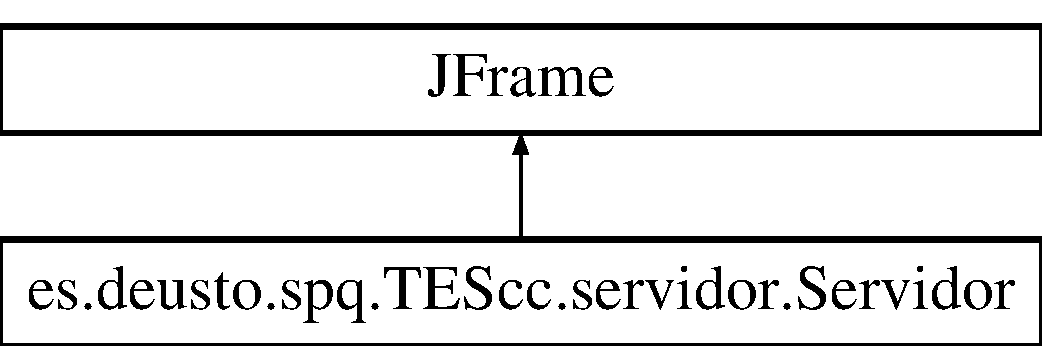
\includegraphics[height=2.000000cm]{classes_1_1deusto_1_1spq_1_1_t_e_scc_1_1servidor_1_1_servidor}
\end{center}
\end{figure}
\subsection*{Métodos públicos}
\begin{DoxyCompactItemize}
\item 
\hyperlink{classes_1_1deusto_1_1spq_1_1_t_e_scc_1_1servidor_1_1_servidor_af99256fabd60a31d22c4fa27f1d96909}{Servidor} (String n, String sn, boolean test)
\end{DoxyCompactItemize}
\subsection*{Métodos públicos estáticos}
\begin{DoxyCompactItemize}
\item 
static void \hyperlink{classes_1_1deusto_1_1spq_1_1_t_e_scc_1_1servidor_1_1_servidor_ad649c5951fc4c399719bdd169d77d6e2}{main} (String\mbox{[}$\,$\mbox{]} args)
\end{DoxyCompactItemize}


\subsection{Descripción detallada}


Definición en la línea 31 del archivo Servidor.\+java.



\subsection{Documentación del constructor y destructor}
\hypertarget{classes_1_1deusto_1_1spq_1_1_t_e_scc_1_1servidor_1_1_servidor_af99256fabd60a31d22c4fa27f1d96909}{\index{es\+::deusto\+::spq\+::\+T\+E\+Scc\+::servidor\+::\+Servidor@{es\+::deusto\+::spq\+::\+T\+E\+Scc\+::servidor\+::\+Servidor}!Servidor@{Servidor}}
\index{Servidor@{Servidor}!es\+::deusto\+::spq\+::\+T\+E\+Scc\+::servidor\+::\+Servidor@{es\+::deusto\+::spq\+::\+T\+E\+Scc\+::servidor\+::\+Servidor}}
\subsubsection[{Servidor}]{\setlength{\rightskip}{0pt plus 5cm}es.\+deusto.\+spq.\+T\+E\+Scc.\+servidor.\+Servidor.\+Servidor (
\begin{DoxyParamCaption}
\item[{String}]{n, }
\item[{String}]{sn, }
\item[{boolean}]{test}
\end{DoxyParamCaption}
)}}\label{classes_1_1deusto_1_1spq_1_1_t_e_scc_1_1servidor_1_1_servidor_af99256fabd60a31d22c4fa27f1d96909}


Definición en la línea 65 del archivo Servidor.\+java.



\subsection{Documentación de las funciones miembro}
\hypertarget{classes_1_1deusto_1_1spq_1_1_t_e_scc_1_1servidor_1_1_servidor_ad649c5951fc4c399719bdd169d77d6e2}{\index{es\+::deusto\+::spq\+::\+T\+E\+Scc\+::servidor\+::\+Servidor@{es\+::deusto\+::spq\+::\+T\+E\+Scc\+::servidor\+::\+Servidor}!main@{main}}
\index{main@{main}!es\+::deusto\+::spq\+::\+T\+E\+Scc\+::servidor\+::\+Servidor@{es\+::deusto\+::spq\+::\+T\+E\+Scc\+::servidor\+::\+Servidor}}
\subsubsection[{main}]{\setlength{\rightskip}{0pt plus 5cm}static void es.\+deusto.\+spq.\+T\+E\+Scc.\+servidor.\+Servidor.\+main (
\begin{DoxyParamCaption}
\item[{String\mbox{[}$\,$\mbox{]}}]{args}
\end{DoxyParamCaption}
)\hspace{0.3cm}{\ttfamily [static]}}}\label{classes_1_1deusto_1_1spq_1_1_t_e_scc_1_1servidor_1_1_servidor_ad649c5951fc4c399719bdd169d77d6e2}


Definición en la línea 41 del archivo Servidor.\+java.



La documentación para esta clase fue generada a partir del siguiente fichero\+:\begin{DoxyCompactItemize}
\item 
src/main/java/es/deusto/spq/\+T\+E\+Scc/servidor/\hyperlink{_servidor_8java}{Servidor.\+java}\end{DoxyCompactItemize}

\hypertarget{classes_1_1deusto_1_1spq_1_1_t_e_scc_1_1servidor_1_1jdo_1_1_usuario}{\section{Referencia de la Clase es.\+deusto.\+spq.\+T\+E\+Scc.\+servidor.\+jdo.\+Usuario}
\label{classes_1_1deusto_1_1spq_1_1_t_e_scc_1_1servidor_1_1jdo_1_1_usuario}\index{es.\+deusto.\+spq.\+T\+E\+Scc.\+servidor.\+jdo.\+Usuario@{es.\+deusto.\+spq.\+T\+E\+Scc.\+servidor.\+jdo.\+Usuario}}
}
\subsection*{Métodos públicos}
\begin{DoxyCompactItemize}
\item 
\hyperlink{classes_1_1deusto_1_1spq_1_1_t_e_scc_1_1servidor_1_1jdo_1_1_usuario_a607ede79f8a7cdee04a8e3de619f1fcf}{Usuario} ()
\item 
\hyperlink{classes_1_1deusto_1_1spq_1_1_t_e_scc_1_1servidor_1_1jdo_1_1_usuario_a137a01fd100dccc041df326ca16caff6}{Usuario} (String nombre, String username, String contrasena)
\item 
String \hyperlink{classes_1_1deusto_1_1spq_1_1_t_e_scc_1_1servidor_1_1jdo_1_1_usuario_aa9175f3107f81ecc9e272a58ff9509d1}{get\+Nombre} ()
\item 
void \hyperlink{classes_1_1deusto_1_1spq_1_1_t_e_scc_1_1servidor_1_1jdo_1_1_usuario_aad7942b71efd65fd7b27d26cab1c2623}{set\+Nombre} (String nombre)
\item 
String \hyperlink{classes_1_1deusto_1_1spq_1_1_t_e_scc_1_1servidor_1_1jdo_1_1_usuario_a82df5180138094f3ed1c692e32b91c72}{get\+Username} ()
\item 
void \hyperlink{classes_1_1deusto_1_1spq_1_1_t_e_scc_1_1servidor_1_1jdo_1_1_usuario_ae4f0449c1f8731b9d7d4f4c71242b1e1}{set\+Username} (String username)
\item 
String \hyperlink{classes_1_1deusto_1_1spq_1_1_t_e_scc_1_1servidor_1_1jdo_1_1_usuario_afd1695e7957e71acbaae97c361216dd5}{get\+Contrasena} ()
\item 
void \hyperlink{classes_1_1deusto_1_1spq_1_1_t_e_scc_1_1servidor_1_1jdo_1_1_usuario_ad9432de1a0c5229aab9d6d669b3c382e}{set\+Contrasena} (String contrasena)
\item 
void \hyperlink{classes_1_1deusto_1_1spq_1_1_t_e_scc_1_1servidor_1_1jdo_1_1_usuario_a6edb840eaaf886da29ace4023f2e3455}{aniadir\+Personaje} (\hyperlink{classes_1_1deusto_1_1spq_1_1_t_e_scc_1_1servidor_1_1jdo_1_1_personaje}{Personaje} personaje)
\item 
void \hyperlink{classes_1_1deusto_1_1spq_1_1_t_e_scc_1_1servidor_1_1jdo_1_1_usuario_a6f982d2b9099e2aa7b27c52cc45f9a78}{eliminar\+Personaje} (\hyperlink{classes_1_1deusto_1_1spq_1_1_t_e_scc_1_1servidor_1_1jdo_1_1_personaje}{Personaje} personaje)
\item 
int \hyperlink{classes_1_1deusto_1_1spq_1_1_t_e_scc_1_1servidor_1_1jdo_1_1_usuario_a0216ecb5838ddd0cbf6eb8de143ff420}{numero\+De\+Personajes} ()
\item 
Set$<$ \hyperlink{classes_1_1deusto_1_1spq_1_1_t_e_scc_1_1servidor_1_1jdo_1_1_personaje}{Personaje} $>$ \hyperlink{classes_1_1deusto_1_1spq_1_1_t_e_scc_1_1servidor_1_1jdo_1_1_usuario_aaadf3c54300a29f8028f16c80593da49}{get\+Personajes} ()
\item 
void \hyperlink{classes_1_1deusto_1_1spq_1_1_t_e_scc_1_1servidor_1_1jdo_1_1_usuario_af691dd3475128ad195124da20527b328}{set\+Personajes} (Set$<$ \hyperlink{classes_1_1deusto_1_1spq_1_1_t_e_scc_1_1servidor_1_1jdo_1_1_personaje}{Personaje} $>$ personajes)
\item 
boolean \hyperlink{classes_1_1deusto_1_1spq_1_1_t_e_scc_1_1servidor_1_1jdo_1_1_usuario_ae27da3566b467b0464817abf9c0c7c5c}{equals} (\hyperlink{classes_1_1deusto_1_1spq_1_1_t_e_scc_1_1servidor_1_1jdo_1_1_usuario}{Usuario} usuario)
\end{DoxyCompactItemize}


\subsection{Descripción detallada}


Definición en la línea 10 del archivo Usuario.\+java.



\subsection{Documentación del constructor y destructor}
\hypertarget{classes_1_1deusto_1_1spq_1_1_t_e_scc_1_1servidor_1_1jdo_1_1_usuario_a607ede79f8a7cdee04a8e3de619f1fcf}{\index{es\+::deusto\+::spq\+::\+T\+E\+Scc\+::servidor\+::jdo\+::\+Usuario@{es\+::deusto\+::spq\+::\+T\+E\+Scc\+::servidor\+::jdo\+::\+Usuario}!Usuario@{Usuario}}
\index{Usuario@{Usuario}!es\+::deusto\+::spq\+::\+T\+E\+Scc\+::servidor\+::jdo\+::\+Usuario@{es\+::deusto\+::spq\+::\+T\+E\+Scc\+::servidor\+::jdo\+::\+Usuario}}
\subsubsection[{Usuario}]{\setlength{\rightskip}{0pt plus 5cm}es.\+deusto.\+spq.\+T\+E\+Scc.\+servidor.\+jdo.\+Usuario.\+Usuario (
\begin{DoxyParamCaption}
{}
\end{DoxyParamCaption}
)}}\label{classes_1_1deusto_1_1spq_1_1_t_e_scc_1_1servidor_1_1jdo_1_1_usuario_a607ede79f8a7cdee04a8e3de619f1fcf}


Definición en la línea 17 del archivo Usuario.\+java.

\hypertarget{classes_1_1deusto_1_1spq_1_1_t_e_scc_1_1servidor_1_1jdo_1_1_usuario_a137a01fd100dccc041df326ca16caff6}{\index{es\+::deusto\+::spq\+::\+T\+E\+Scc\+::servidor\+::jdo\+::\+Usuario@{es\+::deusto\+::spq\+::\+T\+E\+Scc\+::servidor\+::jdo\+::\+Usuario}!Usuario@{Usuario}}
\index{Usuario@{Usuario}!es\+::deusto\+::spq\+::\+T\+E\+Scc\+::servidor\+::jdo\+::\+Usuario@{es\+::deusto\+::spq\+::\+T\+E\+Scc\+::servidor\+::jdo\+::\+Usuario}}
\subsubsection[{Usuario}]{\setlength{\rightskip}{0pt plus 5cm}es.\+deusto.\+spq.\+T\+E\+Scc.\+servidor.\+jdo.\+Usuario.\+Usuario (
\begin{DoxyParamCaption}
\item[{String}]{nombre, }
\item[{String}]{username, }
\item[{String}]{contrasena}
\end{DoxyParamCaption}
)}}\label{classes_1_1deusto_1_1spq_1_1_t_e_scc_1_1servidor_1_1jdo_1_1_usuario_a137a01fd100dccc041df326ca16caff6}


Definición en la línea 21 del archivo Usuario.\+java.



\subsection{Documentación de las funciones miembro}
\hypertarget{classes_1_1deusto_1_1spq_1_1_t_e_scc_1_1servidor_1_1jdo_1_1_usuario_a6edb840eaaf886da29ace4023f2e3455}{\index{es\+::deusto\+::spq\+::\+T\+E\+Scc\+::servidor\+::jdo\+::\+Usuario@{es\+::deusto\+::spq\+::\+T\+E\+Scc\+::servidor\+::jdo\+::\+Usuario}!aniadir\+Personaje@{aniadir\+Personaje}}
\index{aniadir\+Personaje@{aniadir\+Personaje}!es\+::deusto\+::spq\+::\+T\+E\+Scc\+::servidor\+::jdo\+::\+Usuario@{es\+::deusto\+::spq\+::\+T\+E\+Scc\+::servidor\+::jdo\+::\+Usuario}}
\subsubsection[{aniadir\+Personaje}]{\setlength{\rightskip}{0pt plus 5cm}void es.\+deusto.\+spq.\+T\+E\+Scc.\+servidor.\+jdo.\+Usuario.\+aniadir\+Personaje (
\begin{DoxyParamCaption}
\item[{{\bf Personaje}}]{personaje}
\end{DoxyParamCaption}
)}}\label{classes_1_1deusto_1_1spq_1_1_t_e_scc_1_1servidor_1_1jdo_1_1_usuario_a6edb840eaaf886da29ace4023f2e3455}


Definición en la línea 51 del archivo Usuario.\+java.

\hypertarget{classes_1_1deusto_1_1spq_1_1_t_e_scc_1_1servidor_1_1jdo_1_1_usuario_a6f982d2b9099e2aa7b27c52cc45f9a78}{\index{es\+::deusto\+::spq\+::\+T\+E\+Scc\+::servidor\+::jdo\+::\+Usuario@{es\+::deusto\+::spq\+::\+T\+E\+Scc\+::servidor\+::jdo\+::\+Usuario}!eliminar\+Personaje@{eliminar\+Personaje}}
\index{eliminar\+Personaje@{eliminar\+Personaje}!es\+::deusto\+::spq\+::\+T\+E\+Scc\+::servidor\+::jdo\+::\+Usuario@{es\+::deusto\+::spq\+::\+T\+E\+Scc\+::servidor\+::jdo\+::\+Usuario}}
\subsubsection[{eliminar\+Personaje}]{\setlength{\rightskip}{0pt plus 5cm}void es.\+deusto.\+spq.\+T\+E\+Scc.\+servidor.\+jdo.\+Usuario.\+eliminar\+Personaje (
\begin{DoxyParamCaption}
\item[{{\bf Personaje}}]{personaje}
\end{DoxyParamCaption}
)}}\label{classes_1_1deusto_1_1spq_1_1_t_e_scc_1_1servidor_1_1jdo_1_1_usuario_a6f982d2b9099e2aa7b27c52cc45f9a78}


Definición en la línea 55 del archivo Usuario.\+java.

\hypertarget{classes_1_1deusto_1_1spq_1_1_t_e_scc_1_1servidor_1_1jdo_1_1_usuario_ae27da3566b467b0464817abf9c0c7c5c}{\index{es\+::deusto\+::spq\+::\+T\+E\+Scc\+::servidor\+::jdo\+::\+Usuario@{es\+::deusto\+::spq\+::\+T\+E\+Scc\+::servidor\+::jdo\+::\+Usuario}!equals@{equals}}
\index{equals@{equals}!es\+::deusto\+::spq\+::\+T\+E\+Scc\+::servidor\+::jdo\+::\+Usuario@{es\+::deusto\+::spq\+::\+T\+E\+Scc\+::servidor\+::jdo\+::\+Usuario}}
\subsubsection[{equals}]{\setlength{\rightskip}{0pt plus 5cm}boolean es.\+deusto.\+spq.\+T\+E\+Scc.\+servidor.\+jdo.\+Usuario.\+equals (
\begin{DoxyParamCaption}
\item[{{\bf Usuario}}]{usuario}
\end{DoxyParamCaption}
)}}\label{classes_1_1deusto_1_1spq_1_1_t_e_scc_1_1servidor_1_1jdo_1_1_usuario_ae27da3566b467b0464817abf9c0c7c5c}


Definición en la línea 71 del archivo Usuario.\+java.

\hypertarget{classes_1_1deusto_1_1spq_1_1_t_e_scc_1_1servidor_1_1jdo_1_1_usuario_afd1695e7957e71acbaae97c361216dd5}{\index{es\+::deusto\+::spq\+::\+T\+E\+Scc\+::servidor\+::jdo\+::\+Usuario@{es\+::deusto\+::spq\+::\+T\+E\+Scc\+::servidor\+::jdo\+::\+Usuario}!get\+Contrasena@{get\+Contrasena}}
\index{get\+Contrasena@{get\+Contrasena}!es\+::deusto\+::spq\+::\+T\+E\+Scc\+::servidor\+::jdo\+::\+Usuario@{es\+::deusto\+::spq\+::\+T\+E\+Scc\+::servidor\+::jdo\+::\+Usuario}}
\subsubsection[{get\+Contrasena}]{\setlength{\rightskip}{0pt plus 5cm}String es.\+deusto.\+spq.\+T\+E\+Scc.\+servidor.\+jdo.\+Usuario.\+get\+Contrasena (
\begin{DoxyParamCaption}
{}
\end{DoxyParamCaption}
)}}\label{classes_1_1deusto_1_1spq_1_1_t_e_scc_1_1servidor_1_1jdo_1_1_usuario_afd1695e7957e71acbaae97c361216dd5}


Definición en la línea 43 del archivo Usuario.\+java.

\hypertarget{classes_1_1deusto_1_1spq_1_1_t_e_scc_1_1servidor_1_1jdo_1_1_usuario_aa9175f3107f81ecc9e272a58ff9509d1}{\index{es\+::deusto\+::spq\+::\+T\+E\+Scc\+::servidor\+::jdo\+::\+Usuario@{es\+::deusto\+::spq\+::\+T\+E\+Scc\+::servidor\+::jdo\+::\+Usuario}!get\+Nombre@{get\+Nombre}}
\index{get\+Nombre@{get\+Nombre}!es\+::deusto\+::spq\+::\+T\+E\+Scc\+::servidor\+::jdo\+::\+Usuario@{es\+::deusto\+::spq\+::\+T\+E\+Scc\+::servidor\+::jdo\+::\+Usuario}}
\subsubsection[{get\+Nombre}]{\setlength{\rightskip}{0pt plus 5cm}String es.\+deusto.\+spq.\+T\+E\+Scc.\+servidor.\+jdo.\+Usuario.\+get\+Nombre (
\begin{DoxyParamCaption}
{}
\end{DoxyParamCaption}
)}}\label{classes_1_1deusto_1_1spq_1_1_t_e_scc_1_1servidor_1_1jdo_1_1_usuario_aa9175f3107f81ecc9e272a58ff9509d1}


Definición en la línea 27 del archivo Usuario.\+java.

\hypertarget{classes_1_1deusto_1_1spq_1_1_t_e_scc_1_1servidor_1_1jdo_1_1_usuario_aaadf3c54300a29f8028f16c80593da49}{\index{es\+::deusto\+::spq\+::\+T\+E\+Scc\+::servidor\+::jdo\+::\+Usuario@{es\+::deusto\+::spq\+::\+T\+E\+Scc\+::servidor\+::jdo\+::\+Usuario}!get\+Personajes@{get\+Personajes}}
\index{get\+Personajes@{get\+Personajes}!es\+::deusto\+::spq\+::\+T\+E\+Scc\+::servidor\+::jdo\+::\+Usuario@{es\+::deusto\+::spq\+::\+T\+E\+Scc\+::servidor\+::jdo\+::\+Usuario}}
\subsubsection[{get\+Personajes}]{\setlength{\rightskip}{0pt plus 5cm}Set$<${\bf Personaje}$>$ es.\+deusto.\+spq.\+T\+E\+Scc.\+servidor.\+jdo.\+Usuario.\+get\+Personajes (
\begin{DoxyParamCaption}
{}
\end{DoxyParamCaption}
)}}\label{classes_1_1deusto_1_1spq_1_1_t_e_scc_1_1servidor_1_1jdo_1_1_usuario_aaadf3c54300a29f8028f16c80593da49}


Definición en la línea 63 del archivo Usuario.\+java.

\hypertarget{classes_1_1deusto_1_1spq_1_1_t_e_scc_1_1servidor_1_1jdo_1_1_usuario_a82df5180138094f3ed1c692e32b91c72}{\index{es\+::deusto\+::spq\+::\+T\+E\+Scc\+::servidor\+::jdo\+::\+Usuario@{es\+::deusto\+::spq\+::\+T\+E\+Scc\+::servidor\+::jdo\+::\+Usuario}!get\+Username@{get\+Username}}
\index{get\+Username@{get\+Username}!es\+::deusto\+::spq\+::\+T\+E\+Scc\+::servidor\+::jdo\+::\+Usuario@{es\+::deusto\+::spq\+::\+T\+E\+Scc\+::servidor\+::jdo\+::\+Usuario}}
\subsubsection[{get\+Username}]{\setlength{\rightskip}{0pt plus 5cm}String es.\+deusto.\+spq.\+T\+E\+Scc.\+servidor.\+jdo.\+Usuario.\+get\+Username (
\begin{DoxyParamCaption}
{}
\end{DoxyParamCaption}
)}}\label{classes_1_1deusto_1_1spq_1_1_t_e_scc_1_1servidor_1_1jdo_1_1_usuario_a82df5180138094f3ed1c692e32b91c72}


Definición en la línea 35 del archivo Usuario.\+java.

\hypertarget{classes_1_1deusto_1_1spq_1_1_t_e_scc_1_1servidor_1_1jdo_1_1_usuario_a0216ecb5838ddd0cbf6eb8de143ff420}{\index{es\+::deusto\+::spq\+::\+T\+E\+Scc\+::servidor\+::jdo\+::\+Usuario@{es\+::deusto\+::spq\+::\+T\+E\+Scc\+::servidor\+::jdo\+::\+Usuario}!numero\+De\+Personajes@{numero\+De\+Personajes}}
\index{numero\+De\+Personajes@{numero\+De\+Personajes}!es\+::deusto\+::spq\+::\+T\+E\+Scc\+::servidor\+::jdo\+::\+Usuario@{es\+::deusto\+::spq\+::\+T\+E\+Scc\+::servidor\+::jdo\+::\+Usuario}}
\subsubsection[{numero\+De\+Personajes}]{\setlength{\rightskip}{0pt plus 5cm}int es.\+deusto.\+spq.\+T\+E\+Scc.\+servidor.\+jdo.\+Usuario.\+numero\+De\+Personajes (
\begin{DoxyParamCaption}
{}
\end{DoxyParamCaption}
)}}\label{classes_1_1deusto_1_1spq_1_1_t_e_scc_1_1servidor_1_1jdo_1_1_usuario_a0216ecb5838ddd0cbf6eb8de143ff420}


Definición en la línea 59 del archivo Usuario.\+java.

\hypertarget{classes_1_1deusto_1_1spq_1_1_t_e_scc_1_1servidor_1_1jdo_1_1_usuario_ad9432de1a0c5229aab9d6d669b3c382e}{\index{es\+::deusto\+::spq\+::\+T\+E\+Scc\+::servidor\+::jdo\+::\+Usuario@{es\+::deusto\+::spq\+::\+T\+E\+Scc\+::servidor\+::jdo\+::\+Usuario}!set\+Contrasena@{set\+Contrasena}}
\index{set\+Contrasena@{set\+Contrasena}!es\+::deusto\+::spq\+::\+T\+E\+Scc\+::servidor\+::jdo\+::\+Usuario@{es\+::deusto\+::spq\+::\+T\+E\+Scc\+::servidor\+::jdo\+::\+Usuario}}
\subsubsection[{set\+Contrasena}]{\setlength{\rightskip}{0pt plus 5cm}void es.\+deusto.\+spq.\+T\+E\+Scc.\+servidor.\+jdo.\+Usuario.\+set\+Contrasena (
\begin{DoxyParamCaption}
\item[{String}]{contrasena}
\end{DoxyParamCaption}
)}}\label{classes_1_1deusto_1_1spq_1_1_t_e_scc_1_1servidor_1_1jdo_1_1_usuario_ad9432de1a0c5229aab9d6d669b3c382e}


Definición en la línea 47 del archivo Usuario.\+java.

\hypertarget{classes_1_1deusto_1_1spq_1_1_t_e_scc_1_1servidor_1_1jdo_1_1_usuario_aad7942b71efd65fd7b27d26cab1c2623}{\index{es\+::deusto\+::spq\+::\+T\+E\+Scc\+::servidor\+::jdo\+::\+Usuario@{es\+::deusto\+::spq\+::\+T\+E\+Scc\+::servidor\+::jdo\+::\+Usuario}!set\+Nombre@{set\+Nombre}}
\index{set\+Nombre@{set\+Nombre}!es\+::deusto\+::spq\+::\+T\+E\+Scc\+::servidor\+::jdo\+::\+Usuario@{es\+::deusto\+::spq\+::\+T\+E\+Scc\+::servidor\+::jdo\+::\+Usuario}}
\subsubsection[{set\+Nombre}]{\setlength{\rightskip}{0pt plus 5cm}void es.\+deusto.\+spq.\+T\+E\+Scc.\+servidor.\+jdo.\+Usuario.\+set\+Nombre (
\begin{DoxyParamCaption}
\item[{String}]{nombre}
\end{DoxyParamCaption}
)}}\label{classes_1_1deusto_1_1spq_1_1_t_e_scc_1_1servidor_1_1jdo_1_1_usuario_aad7942b71efd65fd7b27d26cab1c2623}


Definición en la línea 31 del archivo Usuario.\+java.

\hypertarget{classes_1_1deusto_1_1spq_1_1_t_e_scc_1_1servidor_1_1jdo_1_1_usuario_af691dd3475128ad195124da20527b328}{\index{es\+::deusto\+::spq\+::\+T\+E\+Scc\+::servidor\+::jdo\+::\+Usuario@{es\+::deusto\+::spq\+::\+T\+E\+Scc\+::servidor\+::jdo\+::\+Usuario}!set\+Personajes@{set\+Personajes}}
\index{set\+Personajes@{set\+Personajes}!es\+::deusto\+::spq\+::\+T\+E\+Scc\+::servidor\+::jdo\+::\+Usuario@{es\+::deusto\+::spq\+::\+T\+E\+Scc\+::servidor\+::jdo\+::\+Usuario}}
\subsubsection[{set\+Personajes}]{\setlength{\rightskip}{0pt plus 5cm}void es.\+deusto.\+spq.\+T\+E\+Scc.\+servidor.\+jdo.\+Usuario.\+set\+Personajes (
\begin{DoxyParamCaption}
\item[{Set$<$ {\bf Personaje} $>$}]{personajes}
\end{DoxyParamCaption}
)}}\label{classes_1_1deusto_1_1spq_1_1_t_e_scc_1_1servidor_1_1jdo_1_1_usuario_af691dd3475128ad195124da20527b328}


Definición en la línea 67 del archivo Usuario.\+java.

\hypertarget{classes_1_1deusto_1_1spq_1_1_t_e_scc_1_1servidor_1_1jdo_1_1_usuario_ae4f0449c1f8731b9d7d4f4c71242b1e1}{\index{es\+::deusto\+::spq\+::\+T\+E\+Scc\+::servidor\+::jdo\+::\+Usuario@{es\+::deusto\+::spq\+::\+T\+E\+Scc\+::servidor\+::jdo\+::\+Usuario}!set\+Username@{set\+Username}}
\index{set\+Username@{set\+Username}!es\+::deusto\+::spq\+::\+T\+E\+Scc\+::servidor\+::jdo\+::\+Usuario@{es\+::deusto\+::spq\+::\+T\+E\+Scc\+::servidor\+::jdo\+::\+Usuario}}
\subsubsection[{set\+Username}]{\setlength{\rightskip}{0pt plus 5cm}void es.\+deusto.\+spq.\+T\+E\+Scc.\+servidor.\+jdo.\+Usuario.\+set\+Username (
\begin{DoxyParamCaption}
\item[{String}]{username}
\end{DoxyParamCaption}
)}}\label{classes_1_1deusto_1_1spq_1_1_t_e_scc_1_1servidor_1_1jdo_1_1_usuario_ae4f0449c1f8731b9d7d4f4c71242b1e1}


Definición en la línea 39 del archivo Usuario.\+java.



La documentación para esta clase fue generada a partir del siguiente fichero\+:\begin{DoxyCompactItemize}
\item 
src/main/java/es/deusto/spq/\+T\+E\+Scc/servidor/jdo/\hyperlink{_usuario_8java}{Usuario.\+java}\end{DoxyCompactItemize}

\hypertarget{classes_1_1deusto_1_1spq_1_1_t_e_scc_1_1utilidades_1_1_utilidades_g_u_i}{\section{Referencia de la Clase es.\+deusto.\+spq.\+T\+E\+Scc.\+utilidades.\+Utilidades\+G\+U\+I}
\label{classes_1_1deusto_1_1spq_1_1_t_e_scc_1_1utilidades_1_1_utilidades_g_u_i}\index{es.\+deusto.\+spq.\+T\+E\+Scc.\+utilidades.\+Utilidades\+G\+U\+I@{es.\+deusto.\+spq.\+T\+E\+Scc.\+utilidades.\+Utilidades\+G\+U\+I}}
}
\subsection*{Métodos públicos estáticos}
\begin{DoxyCompactItemize}
\item 
static Container \hyperlink{classes_1_1deusto_1_1spq_1_1_t_e_scc_1_1utilidades_1_1_utilidades_g_u_i_a383389b6c66cbd659f9647a1bd922de6}{get\+Contenedor\+Principal} (Component c)
\end{DoxyCompactItemize}


\subsection{Descripción detallada}


Definición en la línea 10 del archivo Utilidades\+G\+U\+I.\+java.



\subsection{Documentación de las funciones miembro}
\hypertarget{classes_1_1deusto_1_1spq_1_1_t_e_scc_1_1utilidades_1_1_utilidades_g_u_i_a383389b6c66cbd659f9647a1bd922de6}{\index{es\+::deusto\+::spq\+::\+T\+E\+Scc\+::utilidades\+::\+Utilidades\+G\+U\+I@{es\+::deusto\+::spq\+::\+T\+E\+Scc\+::utilidades\+::\+Utilidades\+G\+U\+I}!get\+Contenedor\+Principal@{get\+Contenedor\+Principal}}
\index{get\+Contenedor\+Principal@{get\+Contenedor\+Principal}!es\+::deusto\+::spq\+::\+T\+E\+Scc\+::utilidades\+::\+Utilidades\+G\+U\+I@{es\+::deusto\+::spq\+::\+T\+E\+Scc\+::utilidades\+::\+Utilidades\+G\+U\+I}}
\subsubsection[{get\+Contenedor\+Principal}]{\setlength{\rightskip}{0pt plus 5cm}static Container es.\+deusto.\+spq.\+T\+E\+Scc.\+utilidades.\+Utilidades\+G\+U\+I.\+get\+Contenedor\+Principal (
\begin{DoxyParamCaption}
\item[{Component}]{c}
\end{DoxyParamCaption}
)\hspace{0.3cm}{\ttfamily [static]}}}\label{classes_1_1deusto_1_1spq_1_1_t_e_scc_1_1utilidades_1_1_utilidades_g_u_i_a383389b6c66cbd659f9647a1bd922de6}


Definición en la línea 12 del archivo Utilidades\+G\+U\+I.\+java.



La documentación para esta clase fue generada a partir del siguiente fichero\+:\begin{DoxyCompactItemize}
\item 
src/main/java/es/deusto/spq/\+T\+E\+Scc/utilidades/\hyperlink{_utilidades_g_u_i_8java}{Utilidades\+G\+U\+I.\+java}\end{DoxyCompactItemize}

\chapter{Documentación de archivos}
\input{_controller_t_e_s_8java}
\hypertarget{_r_m_i_service_locator_8java}{\section{Referencia del Archivo src/main/java/es/deusto/spq/\+T\+E\+Scc/cliente/\+R\+M\+I\+Service\+Locator.java}
\label{_r_m_i_service_locator_8java}\index{src/main/java/es/deusto/spq/\+T\+E\+Scc/cliente/\+R\+M\+I\+Service\+Locator.\+java@{src/main/java/es/deusto/spq/\+T\+E\+Scc/cliente/\+R\+M\+I\+Service\+Locator.\+java}}
}
\subsection*{Clases}
\begin{DoxyCompactItemize}
\item 
class \hyperlink{classes_1_1deusto_1_1spq_1_1_t_e_scc_1_1cliente_1_1_r_m_i_service_locator}{es.\+deusto.\+spq.\+T\+E\+Scc.\+cliente.\+R\+M\+I\+Service\+Locator}
\end{DoxyCompactItemize}
\subsection*{Paquetes}
\begin{DoxyCompactItemize}
\item 
package \hyperlink{namespacees_1_1deusto_1_1spq_1_1_t_e_scc_1_1cliente}{es.\+deusto.\+spq.\+T\+E\+Scc.\+cliente}
\end{DoxyCompactItemize}

\hypertarget{_objeto_assembler_8java}{\section{Referencia del Archivo src/main/java/es/deusto/spq/\+T\+E\+Scc/dto/\+Objeto\+Assembler.java}
\label{_objeto_assembler_8java}\index{src/main/java/es/deusto/spq/\+T\+E\+Scc/dto/\+Objeto\+Assembler.\+java@{src/main/java/es/deusto/spq/\+T\+E\+Scc/dto/\+Objeto\+Assembler.\+java}}
}
\subsection*{Clases}
\begin{DoxyCompactItemize}
\item 
class \hyperlink{classes_1_1deusto_1_1spq_1_1_t_e_scc_1_1dto_1_1_objeto_assembler}{es.\+deusto.\+spq.\+T\+E\+Scc.\+dto.\+Objeto\+Assembler}
\end{DoxyCompactItemize}
\subsection*{Paquetes}
\begin{DoxyCompactItemize}
\item 
package \hyperlink{namespacees_1_1deusto_1_1spq_1_1_t_e_scc_1_1dto}{es.\+deusto.\+spq.\+T\+E\+Scc.\+dto}
\end{DoxyCompactItemize}

\hypertarget{_objeto_d_t_o_8java}{\section{Referencia del Archivo src/main/java/es/deusto/spq/\+T\+E\+Scc/dto/\+Objeto\+D\+T\+O.java}
\label{_objeto_d_t_o_8java}\index{src/main/java/es/deusto/spq/\+T\+E\+Scc/dto/\+Objeto\+D\+T\+O.\+java@{src/main/java/es/deusto/spq/\+T\+E\+Scc/dto/\+Objeto\+D\+T\+O.\+java}}
}
\subsection*{Clases}
\begin{DoxyCompactItemize}
\item 
class \hyperlink{classes_1_1deusto_1_1spq_1_1_t_e_scc_1_1dto_1_1_objeto_d_t_o}{es.\+deusto.\+spq.\+T\+E\+Scc.\+dto.\+Objeto\+D\+T\+O}
\end{DoxyCompactItemize}
\subsection*{Paquetes}
\begin{DoxyCompactItemize}
\item 
package \hyperlink{namespacees_1_1deusto_1_1spq_1_1_t_e_scc_1_1dto}{es.\+deusto.\+spq.\+T\+E\+Scc.\+dto}
\end{DoxyCompactItemize}

\hypertarget{_personaje_assembler_8java}{\section{Referencia del Archivo src/main/java/es/deusto/spq/\+T\+E\+Scc/dto/\+Personaje\+Assembler.java}
\label{_personaje_assembler_8java}\index{src/main/java/es/deusto/spq/\+T\+E\+Scc/dto/\+Personaje\+Assembler.\+java@{src/main/java/es/deusto/spq/\+T\+E\+Scc/dto/\+Personaje\+Assembler.\+java}}
}
\subsection*{Clases}
\begin{DoxyCompactItemize}
\item 
class \hyperlink{classes_1_1deusto_1_1spq_1_1_t_e_scc_1_1dto_1_1_personaje_assembler}{es.\+deusto.\+spq.\+T\+E\+Scc.\+dto.\+Personaje\+Assembler}
\end{DoxyCompactItemize}
\subsection*{Paquetes}
\begin{DoxyCompactItemize}
\item 
package \hyperlink{namespacees_1_1deusto_1_1spq_1_1_t_e_scc_1_1dto}{es.\+deusto.\+spq.\+T\+E\+Scc.\+dto}
\end{DoxyCompactItemize}

\hypertarget{_personaje_d_t_o_8java}{\section{Referencia del Archivo src/main/java/es/deusto/spq/\+T\+E\+Scc/dto/\+Personaje\+D\+T\+O.java}
\label{_personaje_d_t_o_8java}\index{src/main/java/es/deusto/spq/\+T\+E\+Scc/dto/\+Personaje\+D\+T\+O.\+java@{src/main/java/es/deusto/spq/\+T\+E\+Scc/dto/\+Personaje\+D\+T\+O.\+java}}
}
\subsection*{Clases}
\begin{DoxyCompactItemize}
\item 
class \hyperlink{classes_1_1deusto_1_1spq_1_1_t_e_scc_1_1dto_1_1_personaje_d_t_o}{es.\+deusto.\+spq.\+T\+E\+Scc.\+dto.\+Personaje\+D\+T\+O}
\end{DoxyCompactItemize}
\subsection*{Paquetes}
\begin{DoxyCompactItemize}
\item 
package \hyperlink{namespacees_1_1deusto_1_1spq_1_1_t_e_scc_1_1dto}{es.\+deusto.\+spq.\+T\+E\+Scc.\+dto}
\end{DoxyCompactItemize}

\hypertarget{_d_a_o_database_8java}{\section{Referencia del Archivo src/main/java/es/deusto/spq/\+T\+E\+Scc/servidor/\+D\+A\+O\+Database.java}
\label{_d_a_o_database_8java}\index{src/main/java/es/deusto/spq/\+T\+E\+Scc/servidor/\+D\+A\+O\+Database.\+java@{src/main/java/es/deusto/spq/\+T\+E\+Scc/servidor/\+D\+A\+O\+Database.\+java}}
}
\subsection*{Clases}
\begin{DoxyCompactItemize}
\item 
class \hyperlink{classes_1_1deusto_1_1spq_1_1_t_e_scc_1_1servidor_1_1_d_a_o_database}{es.\+deusto.\+spq.\+T\+E\+Scc.\+servidor.\+D\+A\+O\+Database}
\end{DoxyCompactItemize}
\subsection*{Paquetes}
\begin{DoxyCompactItemize}
\item 
package \hyperlink{namespacees_1_1deusto_1_1spq_1_1_t_e_scc_1_1servidor}{es.\+deusto.\+spq.\+T\+E\+Scc.\+servidor}
\end{DoxyCompactItemize}

\hypertarget{_facade_8java}{\section{Referencia del Archivo src/main/java/es/deusto/spq/\+T\+E\+Scc/servidor/\+Facade.java}
\label{_facade_8java}\index{src/main/java/es/deusto/spq/\+T\+E\+Scc/servidor/\+Facade.\+java@{src/main/java/es/deusto/spq/\+T\+E\+Scc/servidor/\+Facade.\+java}}
}
\subsection*{Clases}
\begin{DoxyCompactItemize}
\item 
class \hyperlink{classes_1_1deusto_1_1spq_1_1_t_e_scc_1_1servidor_1_1_facade}{es.\+deusto.\+spq.\+T\+E\+Scc.\+servidor.\+Facade}
\end{DoxyCompactItemize}
\subsection*{Paquetes}
\begin{DoxyCompactItemize}
\item 
package \hyperlink{namespacees_1_1deusto_1_1spq_1_1_t_e_scc_1_1servidor}{es.\+deusto.\+spq.\+T\+E\+Scc.\+servidor}
\end{DoxyCompactItemize}

\hypertarget{_i_facade_8java}{\section{Referencia del Archivo src/main/java/es/deusto/spq/\+T\+E\+Scc/servidor/\+I\+Facade.java}
\label{_i_facade_8java}\index{src/main/java/es/deusto/spq/\+T\+E\+Scc/servidor/\+I\+Facade.\+java@{src/main/java/es/deusto/spq/\+T\+E\+Scc/servidor/\+I\+Facade.\+java}}
}
\subsection*{Clases}
\begin{DoxyCompactItemize}
\item 
interface \hyperlink{interfacees_1_1deusto_1_1spq_1_1_t_e_scc_1_1servidor_1_1_i_facade}{es.\+deusto.\+spq.\+T\+E\+Scc.\+servidor.\+I\+Facade}
\end{DoxyCompactItemize}
\subsection*{Paquetes}
\begin{DoxyCompactItemize}
\item 
package \hyperlink{namespacees_1_1deusto_1_1spq_1_1_t_e_scc_1_1servidor}{es.\+deusto.\+spq.\+T\+E\+Scc.\+servidor}
\end{DoxyCompactItemize}

\hypertarget{_objeto_8java}{\section{Referencia del Archivo src/main/java/es/deusto/spq/\+T\+E\+Scc/servidor/jdo/\+Objeto.java}
\label{_objeto_8java}\index{src/main/java/es/deusto/spq/\+T\+E\+Scc/servidor/jdo/\+Objeto.\+java@{src/main/java/es/deusto/spq/\+T\+E\+Scc/servidor/jdo/\+Objeto.\+java}}
}
\subsection*{Clases}
\begin{DoxyCompactItemize}
\item 
class \hyperlink{classes_1_1deusto_1_1spq_1_1_t_e_scc_1_1servidor_1_1jdo_1_1_objeto}{es.\+deusto.\+spq.\+T\+E\+Scc.\+servidor.\+jdo.\+Objeto}
\end{DoxyCompactItemize}
\subsection*{Paquetes}
\begin{DoxyCompactItemize}
\item 
package \hyperlink{namespacees_1_1deusto_1_1spq_1_1_t_e_scc_1_1servidor_1_1jdo}{es.\+deusto.\+spq.\+T\+E\+Scc.\+servidor.\+jdo}
\end{DoxyCompactItemize}

\hypertarget{_personaje_8java}{\section{Referencia del Archivo src/main/java/es/deusto/spq/\+T\+E\+Scc/servidor/jdo/\+Personaje.java}
\label{_personaje_8java}\index{src/main/java/es/deusto/spq/\+T\+E\+Scc/servidor/jdo/\+Personaje.\+java@{src/main/java/es/deusto/spq/\+T\+E\+Scc/servidor/jdo/\+Personaje.\+java}}
}
\subsection*{Clases}
\begin{DoxyCompactItemize}
\item 
class \hyperlink{classes_1_1deusto_1_1spq_1_1_t_e_scc_1_1servidor_1_1jdo_1_1_personaje}{es.\+deusto.\+spq.\+T\+E\+Scc.\+servidor.\+jdo.\+Personaje}
\end{DoxyCompactItemize}
\subsection*{Paquetes}
\begin{DoxyCompactItemize}
\item 
package \hyperlink{namespacees_1_1deusto_1_1spq_1_1_t_e_scc_1_1servidor_1_1jdo}{es.\+deusto.\+spq.\+T\+E\+Scc.\+servidor.\+jdo}
\end{DoxyCompactItemize}

\hypertarget{_usuario_8java}{\section{Referencia del Archivo src/main/java/es/deusto/spq/\+T\+E\+Scc/servidor/jdo/\+Usuario.java}
\label{_usuario_8java}\index{src/main/java/es/deusto/spq/\+T\+E\+Scc/servidor/jdo/\+Usuario.\+java@{src/main/java/es/deusto/spq/\+T\+E\+Scc/servidor/jdo/\+Usuario.\+java}}
}
\subsection*{Clases}
\begin{DoxyCompactItemize}
\item 
class \hyperlink{classes_1_1deusto_1_1spq_1_1_t_e_scc_1_1servidor_1_1jdo_1_1_usuario}{es.\+deusto.\+spq.\+T\+E\+Scc.\+servidor.\+jdo.\+Usuario}
\end{DoxyCompactItemize}
\subsection*{Paquetes}
\begin{DoxyCompactItemize}
\item 
package \hyperlink{namespacees_1_1deusto_1_1spq_1_1_t_e_scc_1_1servidor_1_1jdo}{es.\+deusto.\+spq.\+T\+E\+Scc.\+servidor.\+jdo}
\end{DoxyCompactItemize}

\hypertarget{_servicio_t_e_s_8java}{\section{Referencia del Archivo src/main/java/es/deusto/spq/\+T\+E\+Scc/servidor/\+Servicio\+T\+E\+S.java}
\label{_servicio_t_e_s_8java}\index{src/main/java/es/deusto/spq/\+T\+E\+Scc/servidor/\+Servicio\+T\+E\+S.\+java@{src/main/java/es/deusto/spq/\+T\+E\+Scc/servidor/\+Servicio\+T\+E\+S.\+java}}
}
\subsection*{Clases}
\begin{DoxyCompactItemize}
\item 
class \hyperlink{classes_1_1deusto_1_1spq_1_1_t_e_scc_1_1servidor_1_1_servicio_t_e_s}{es.\+deusto.\+spq.\+T\+E\+Scc.\+servidor.\+Servicio\+T\+E\+S}
\end{DoxyCompactItemize}
\subsection*{Paquetes}
\begin{DoxyCompactItemize}
\item 
package \hyperlink{namespacees_1_1deusto_1_1spq_1_1_t_e_scc_1_1servidor}{es.\+deusto.\+spq.\+T\+E\+Scc.\+servidor}
\end{DoxyCompactItemize}

\hypertarget{_servidor_8java}{\section{Referencia del Archivo src/main/java/es/deusto/spq/\+T\+E\+Scc/servidor/\+Servidor.java}
\label{_servidor_8java}\index{src/main/java/es/deusto/spq/\+T\+E\+Scc/servidor/\+Servidor.\+java@{src/main/java/es/deusto/spq/\+T\+E\+Scc/servidor/\+Servidor.\+java}}
}
\subsection*{Clases}
\begin{DoxyCompactItemize}
\item 
class \hyperlink{classes_1_1deusto_1_1spq_1_1_t_e_scc_1_1servidor_1_1_servidor}{es.\+deusto.\+spq.\+T\+E\+Scc.\+servidor.\+Servidor}
\end{DoxyCompactItemize}
\subsection*{Paquetes}
\begin{DoxyCompactItemize}
\item 
package \hyperlink{namespacees_1_1deusto_1_1spq_1_1_t_e_scc_1_1servidor}{es.\+deusto.\+spq.\+T\+E\+Scc.\+servidor}
\end{DoxyCompactItemize}

\hypertarget{_gui_utility_8java}{\section{Referencia del Archivo src/main/java/es/deusto/spq/\+T\+E\+Scc/utilidades/\+Gui\+Utility.java}
\label{_gui_utility_8java}\index{src/main/java/es/deusto/spq/\+T\+E\+Scc/utilidades/\+Gui\+Utility.\+java@{src/main/java/es/deusto/spq/\+T\+E\+Scc/utilidades/\+Gui\+Utility.\+java}}
}
\subsection*{Clases}
\begin{DoxyCompactItemize}
\item 
class \hyperlink{classes_1_1deusto_1_1spq_1_1_t_e_scc_1_1utilidades_1_1_gui_utility}{es.\+deusto.\+spq.\+T\+E\+Scc.\+utilidades.\+Gui\+Utility}
\end{DoxyCompactItemize}
\subsection*{Paquetes}
\begin{DoxyCompactItemize}
\item 
package \hyperlink{namespacees_1_1deusto_1_1spq_1_1_t_e_scc_1_1utilidades}{es.\+deusto.\+spq.\+T\+E\+Scc.\+utilidades}
\end{DoxyCompactItemize}

\input{_j_splash_8java}
\hypertarget{_j_splash_label_8java}{\section{Referencia del Archivo src/main/java/es/deusto/spq/\+T\+E\+Scc/utilidades/\+J\+Splash\+Label.java}
\label{_j_splash_label_8java}\index{src/main/java/es/deusto/spq/\+T\+E\+Scc/utilidades/\+J\+Splash\+Label.\+java@{src/main/java/es/deusto/spq/\+T\+E\+Scc/utilidades/\+J\+Splash\+Label.\+java}}
}
\subsection*{Clases}
\begin{DoxyCompactItemize}
\item 
class \hyperlink{classes_1_1deusto_1_1spq_1_1_t_e_scc_1_1utilidades_1_1_j_splash_label}{es.\+deusto.\+spq.\+T\+E\+Scc.\+utilidades.\+J\+Splash\+Label}
\end{DoxyCompactItemize}
\subsection*{Paquetes}
\begin{DoxyCompactItemize}
\item 
package \hyperlink{namespacees_1_1deusto_1_1spq_1_1_t_e_scc_1_1utilidades}{es.\+deusto.\+spq.\+T\+E\+Scc.\+utilidades}
\end{DoxyCompactItemize}

\hypertarget{_utilidades_g_u_i_8java}{\section{Referencia del Archivo src/main/java/es/deusto/spq/\+T\+E\+Scc/utilidades/\+Utilidades\+G\+U\+I.java}
\label{_utilidades_g_u_i_8java}\index{src/main/java/es/deusto/spq/\+T\+E\+Scc/utilidades/\+Utilidades\+G\+U\+I.\+java@{src/main/java/es/deusto/spq/\+T\+E\+Scc/utilidades/\+Utilidades\+G\+U\+I.\+java}}
}
\subsection*{Clases}
\begin{DoxyCompactItemize}
\item 
class \hyperlink{classes_1_1deusto_1_1spq_1_1_t_e_scc_1_1utilidades_1_1_utilidades_g_u_i}{es.\+deusto.\+spq.\+T\+E\+Scc.\+utilidades.\+Utilidades\+G\+U\+I}
\end{DoxyCompactItemize}
\subsection*{Paquetes}
\begin{DoxyCompactItemize}
\item 
package \hyperlink{namespacees_1_1deusto_1_1spq_1_1_t_e_scc_1_1utilidades}{es.\+deusto.\+spq.\+T\+E\+Scc.\+utilidades}
\end{DoxyCompactItemize}

\hypertarget{_frame_8java}{\section{Referencia del Archivo src/main/java/es/deusto/spq/\+T\+E\+Scc/ventanas/\+Frame.java}
\label{_frame_8java}\index{src/main/java/es/deusto/spq/\+T\+E\+Scc/ventanas/\+Frame.\+java@{src/main/java/es/deusto/spq/\+T\+E\+Scc/ventanas/\+Frame.\+java}}
}
\subsection*{Clases}
\begin{DoxyCompactItemize}
\item 
class \hyperlink{classes_1_1deusto_1_1spq_1_1_t_e_scc_1_1ventanas_1_1_frame}{es.\+deusto.\+spq.\+T\+E\+Scc.\+ventanas.\+Frame}
\end{DoxyCompactItemize}
\subsection*{Paquetes}
\begin{DoxyCompactItemize}
\item 
package \hyperlink{namespacees_1_1deusto_1_1spq_1_1_t_e_scc_1_1ventanas}{es.\+deusto.\+spq.\+T\+E\+Scc.\+ventanas}
\end{DoxyCompactItemize}

\hypertarget{_menu_personaje_8java}{\section{Referencia del Archivo src/main/java/es/deusto/spq/\+T\+E\+Scc/ventanas/\+Menu\+Personaje.java}
\label{_menu_personaje_8java}\index{src/main/java/es/deusto/spq/\+T\+E\+Scc/ventanas/\+Menu\+Personaje.\+java@{src/main/java/es/deusto/spq/\+T\+E\+Scc/ventanas/\+Menu\+Personaje.\+java}}
}
\subsection*{Clases}
\begin{DoxyCompactItemize}
\item 
class \hyperlink{classes_1_1deusto_1_1spq_1_1_t_e_scc_1_1ventanas_1_1_menu_personaje}{es.\+deusto.\+spq.\+T\+E\+Scc.\+ventanas.\+Menu\+Personaje}
\end{DoxyCompactItemize}
\subsection*{Paquetes}
\begin{DoxyCompactItemize}
\item 
package \hyperlink{namespacees_1_1deusto_1_1spq_1_1_t_e_scc_1_1ventanas}{es.\+deusto.\+spq.\+T\+E\+Scc.\+ventanas}
\end{DoxyCompactItemize}

\hypertarget{_pantalla_carga_inicial_8java}{\section{Referencia del Archivo src/main/java/es/deusto/spq/\+T\+E\+Scc/ventanas/\+Pantalla\+Carga\+Inicial.java}
\label{_pantalla_carga_inicial_8java}\index{src/main/java/es/deusto/spq/\+T\+E\+Scc/ventanas/\+Pantalla\+Carga\+Inicial.\+java@{src/main/java/es/deusto/spq/\+T\+E\+Scc/ventanas/\+Pantalla\+Carga\+Inicial.\+java}}
}
\subsection*{Clases}
\begin{DoxyCompactItemize}
\item 
class \hyperlink{classes_1_1deusto_1_1spq_1_1_t_e_scc_1_1ventanas_1_1_pantalla_carga_inicial}{es.\+deusto.\+spq.\+T\+E\+Scc.\+ventanas.\+Pantalla\+Carga\+Inicial}
\end{DoxyCompactItemize}
\subsection*{Paquetes}
\begin{DoxyCompactItemize}
\item 
package \hyperlink{namespacees_1_1deusto_1_1spq_1_1_t_e_scc_1_1ventanas}{es.\+deusto.\+spq.\+T\+E\+Scc.\+ventanas}
\end{DoxyCompactItemize}

\hypertarget{_pantalla_inicio_8java}{\section{Referencia del Archivo src/main/java/es/deusto/spq/\+T\+E\+Scc/ventanas/\+Pantalla\+Inicio.java}
\label{_pantalla_inicio_8java}\index{src/main/java/es/deusto/spq/\+T\+E\+Scc/ventanas/\+Pantalla\+Inicio.\+java@{src/main/java/es/deusto/spq/\+T\+E\+Scc/ventanas/\+Pantalla\+Inicio.\+java}}
}
\subsection*{Clases}
\begin{DoxyCompactItemize}
\item 
class \hyperlink{classes_1_1deusto_1_1spq_1_1_t_e_scc_1_1ventanas_1_1_pantalla_inicio}{es.\+deusto.\+spq.\+T\+E\+Scc.\+ventanas.\+Pantalla\+Inicio}
\end{DoxyCompactItemize}
\subsection*{Paquetes}
\begin{DoxyCompactItemize}
\item 
package \hyperlink{namespacees_1_1deusto_1_1spq_1_1_t_e_scc_1_1ventanas}{es.\+deusto.\+spq.\+T\+E\+Scc.\+ventanas}
\end{DoxyCompactItemize}

\hypertarget{_pantalla_login_8java}{\section{Referencia del Archivo src/main/java/es/deusto/spq/\+T\+E\+Scc/ventanas/\+Pantalla\+Login.java}
\label{_pantalla_login_8java}\index{src/main/java/es/deusto/spq/\+T\+E\+Scc/ventanas/\+Pantalla\+Login.\+java@{src/main/java/es/deusto/spq/\+T\+E\+Scc/ventanas/\+Pantalla\+Login.\+java}}
}
\subsection*{Clases}
\begin{DoxyCompactItemize}
\item 
class \hyperlink{classes_1_1deusto_1_1spq_1_1_t_e_scc_1_1ventanas_1_1_pantalla_login}{es.\+deusto.\+spq.\+T\+E\+Scc.\+ventanas.\+Pantalla\+Login}
\end{DoxyCompactItemize}
\subsection*{Paquetes}
\begin{DoxyCompactItemize}
\item 
package \hyperlink{namespacees_1_1deusto_1_1spq_1_1_t_e_scc_1_1ventanas}{es.\+deusto.\+spq.\+T\+E\+Scc.\+ventanas}
\end{DoxyCompactItemize}

\hypertarget{_pantalla_registro_8java}{\section{Referencia del Archivo src/main/java/es/deusto/spq/\+T\+E\+Scc/ventanas/\+Pantalla\+Registro.java}
\label{_pantalla_registro_8java}\index{src/main/java/es/deusto/spq/\+T\+E\+Scc/ventanas/\+Pantalla\+Registro.\+java@{src/main/java/es/deusto/spq/\+T\+E\+Scc/ventanas/\+Pantalla\+Registro.\+java}}
}
\subsection*{Clases}
\begin{DoxyCompactItemize}
\item 
class \hyperlink{classes_1_1deusto_1_1spq_1_1_t_e_scc_1_1ventanas_1_1_pantalla_registro}{es.\+deusto.\+spq.\+T\+E\+Scc.\+ventanas.\+Pantalla\+Registro}
\end{DoxyCompactItemize}
\subsection*{Paquetes}
\begin{DoxyCompactItemize}
\item 
package \hyperlink{namespacees_1_1deusto_1_1spq_1_1_t_e_scc_1_1ventanas}{es.\+deusto.\+spq.\+T\+E\+Scc.\+ventanas}
\end{DoxyCompactItemize}

\hypertarget{_pantalla_tabla_personaje_8java}{\section{Referencia del Archivo src/main/java/es/deusto/spq/\+T\+E\+Scc/ventanas/\+Pantalla\+Tabla\+Personaje.java}
\label{_pantalla_tabla_personaje_8java}\index{src/main/java/es/deusto/spq/\+T\+E\+Scc/ventanas/\+Pantalla\+Tabla\+Personaje.\+java@{src/main/java/es/deusto/spq/\+T\+E\+Scc/ventanas/\+Pantalla\+Tabla\+Personaje.\+java}}
}
\subsection*{Clases}
\begin{DoxyCompactItemize}
\item 
class \hyperlink{classes_1_1deusto_1_1spq_1_1_t_e_scc_1_1ventanas_1_1_pantalla_tabla_personaje}{es.\+deusto.\+spq.\+T\+E\+Scc.\+ventanas.\+Pantalla\+Tabla\+Personaje}
\end{DoxyCompactItemize}
\subsection*{Paquetes}
\begin{DoxyCompactItemize}
\item 
package \hyperlink{namespacees_1_1deusto_1_1spq_1_1_t_e_scc_1_1ventanas}{es.\+deusto.\+spq.\+T\+E\+Scc.\+ventanas}
\end{DoxyCompactItemize}

%--- End generated contents ---

% Index
\newpage
\phantomsection
\addcontentsline{toc}{chapter}{Índice}
\printindex

\end{document}
